% PREAMBULE

%package obligatoire : type de document
\documentclass[a4paper,12pt,twoside]{book}

%paquet pour pouvoir charger plus de paquets
\usepackage{morewrites} 

%encodage
\usepackage{fontspec}
\usepackage[utf8]{inputenc}
\usepackage{textcomp}
\makeatletter\@removefromreset{footnote}{chapter}\makeatother


%le package hyperref avec des options
\usepackage[xetex]{hyperref}
\hypersetup{pdfinfo={Title={L’étude des livres d’heures à la lumière du numérique
Le cycle de vie des données et des métadonnées – Analyser, Modéliser, Structurer, Visualiser}, Subject={Mémoire TNAH},NewKey={Livres d'heures, données, métadonnées, machine learning}}}
\usepackage{xunicode}

%déclaration des langues du texte
\usepackage[english,french]{babel}

%paquet pour mettre index et bib dans la toc
\usepackage{tocbibind}

%paquet pour gérer les en-têtes et les pieds de page 
\usepackage{fancyhdr}
\pagestyle{fancy}
\fancyhead[LE]{}
%\fancyhead[RE]{Chapitre~\thechapter}
\renewcommand{\chaptermark}[1]{\markboth{#1}{}}
\fancyhead[LO]{\rightmark}
\fancyhead[RO]{}
%numéro de page en bas centré
\fancyfoot[C]{\textbf{\thepage}}

%paquet pour les notes de bas de page
\usepackage[bottom]{footmisc}

%paquet qui permet de barrer du texte
\usepackage{soul}

%paquet pour mettre du texte en colonnes sur une même page
\usepackage{multicol}

%paquets pour écrire du code coloré
\usepackage{minted}
\usepackage{keyval}
\usepackage{fancyvrb}
\usepackage{xcolor}
\usepackage{ifthen}
\usepackage{calc}
\usepackage{ifplatform}

%paquet pour insérer du code source
\usepackage{listings}

%paquet pour mettre une partie de texte entre commentaire
\usepackage{comment}

%paquet image
\usepackage{wrapfig}
\usepackage{graphicx}
\usepackage{float}

%Paquet tableau
\usepackage{longtable}
\usepackage{colortbl}
\usepackage{diagbox}
\usepackage{array}

%mode paysage
\usepackage{lscape}

%paquet pour inclure des pdf de plusieurs pages
\usepackage{pdfpages}

%configurer le document selon les normes de l'école
\usepackage[margin=2.5cm]{geometry} %marges
\usepackage{setspace} % espacement qui permet ensuite de définir un interligne
\onehalfspacing % interligne de 1.5
\setlength\parindent{1cm} % indentation des paragraphes à 1 cm

\usepackage{lettrine} % lettrines (pas obligatoire)


%bibliographie
\usepackage{csquotes}
\usepackage[backend=biber,sorting=nyt,style=enc]{biblatex}
\addbibresource{Bibliographie.bib}
\nocite{*}

%si index, package pour index + makeindex

% + toutes la liste des packages nécessaires à votre document (si images, tableaux, schémas, etc.)

% on pourra aussi utiliser les commandes qu'on a vues pour enlever les titres courants sur les pages vides

\author{Gwenaëlle Patat - M2 TNAH}
\title{L’étude des livres d’heures à la lumière du numérique
Le cycle de vie des données et des métadonnées – Analyser, Modéliser, Structurer, Visualiser}



% DOCUMENT
\begin{document}
	\frontmatter
	\begin{titlepage}
		\begin{center}
			
			\bigskip
			
			\begin{large}
				\'ÉCOLE NATIONALE DES CHARTES
			\end{large}
			\begin{center}\rule{2cm}{0.02cm}\end{center}
			
			\bigskip
			\bigskip
			\bigskip
			\begin{Large}
				\textbf{Gwenaëlle Patat}\\
			\end{Large}
		%selon le cas
			\begin{normalsize} \textit{Licenciée ès lettres modernes et histoire}\\
				\textit{Diplômée du master \og{}Mondes médiévaux\fg{}}
			\end{normalsize}
			
			\bigskip
			\bigskip
			\bigskip
			
			\begin{Huge}
				\textbf{L’étude des livres d’heures à la lumière du numérique}\\
			\end{Huge}
			\bigskip
			\bigskip
			\begin{LARGE}
				\textbf{Le cycle de vie des données et des métadonnées – Analyser, Modéliser, Structurer, Visualiser.}\\
			\end{LARGE}
			
			\bigskip
			\bigskip
			\bigskip
			\begin{large}
			\end{large}
			\vfill
			
			\begin{large}
				Mémoire 
				pour le diplôme de master \\
				\og{} Technologies numériques appliquées à l'histoire \fg{} \\
				\bigskip
				2020
			\end{large}
			
		\end{center}
	\end{titlepage}
	
	\thispagestyle{empty}	
	\cleardoublepage
	
	\chapter*{Résumé}
	\addcontentsline{toc}{chapter}{Résumé}
	\medskip
	Ce mémoire est le fruit d'une réflexion autour de problématiques abordées lors de mon stage à l'IRHT dans le cadre du projet HORAE, projet qui propose d'étudier les pratiques religieuses de la fin du Moyen Âge à travers les livres d'heures. Le stage s'est concentré sur la production de données de qualité pour la recherche historique, ce qui nous a amené à réfléchir aux stratégies de développement pour la structure, la modélisation, la conversion et la présentation ergonomique des données et des métadonnées, avec le souci constant de garantir leur interopérabilité et leur pérennité. La participation au projet HORAE, qui s'inscrit pleinement dans les Humanités numériques, nous a permis de cerner les apports, les limites et les promesses d'évolution du numérique dans la recherche en sciences humaines et sociales.\\
	
	\textbf{Mots-clés~:} Formats et structuration automatique des données et métadonnées ; livres d'heures ; usages liturgiques ; dévotion au Moyen-Âge ; gestion et management de projet en Humanités numériques ; Reconnaissance automatique de texte ; \textit{Handwritten Text Recognition} ; \textit{Optical Character Recognition} ; Interopérabilité ; XML-TEI ; XSLT ; ODD ; Schematron ; Python ; \textit{Machine learning} ; Ergonomie ; Modélisation ; Base de données relationnelles.\\
	
	\textbf{Informations bibliographiques~:} Gwenaëlle Patat, \textit{L’étude des livres d’heures à la lumière du numérique. Le cycle de vie des données et des métadonnées – Analyser, Modéliser, Structurer, Visualiser}, mémoire de master \og{}Technologies numériques appliquées à l'histoire\fg{}, dir. Jean-Baptiste Camps et Dominique Stutzmann, École nationale des Chartes, 2020.
	
	\chapter*{Remerciements}
	\addcontentsline{toc}{chapter}{Remerciements}
	
	\lettrine{M}es remerciements vont tout d'abord à l'équipe de l'IRHT qui m'a accueillie et m'a intégrée à ses réunions quotidiennes : bien évidemment mon tuteur Dominique Stutzmann, qui a eu la patience de stimuler ma réflexion et de me faire part de sa rigueur et de son exigence. Je remercie également les deux autres membres de l'équipe HORAE, Laura Lebarbey et Louis Chevalier, pour avoir répondu avec enthousiasme à mes doutes et à mes questions, ainsi que Sergio Torres et Ian Johnson pour leur aide et leurs conseils techniques. Je souhaite également remercier l'équipe de Teklia pour m'avoir apporté des précisions sur le projet et les problématiques relatives au \textit{machine learning}.\\
	
	Je tiens à remercier l'ensemble des professeurs et intervenants qui nous ont formés lors de cette année de master, en particulier mon tuteur Jean-Baptiste Camps, ainsi que Thibault Clérice, Ariane Pinche, Gautier Poupeau et Rémy Delmotte pour avoir répondu à mes questions et apporté leur soutien durant le stage. Merci également à Laura Albiero, avec qui j'ai eu la chance d'échanger lors d'une formation continue en septembre dernier.\\
	
	Enfin, je remercie chaleureusement Catherine Patat, Alain Patat et Marie Millarec pour leur relecture, ainsi que l'ensemble de la promotion 2020 dans laquelle la solidarité et la stimulation intellectuelle n'ont pas manqué, en particulier Jean-Luc Mirepoix et Chloë Fize pour leur aide et leur soutien sans faille. 

    \newpage
	%bibliographie ici
	%\printbibliography[title=Bibliographie]
	\chapter*{Bibliographie}
	    \printbibliography[heading=subbibliography,keyword={MA},title={Manuscrits, livres d'heures, liturgie et dévotion au Moyen Âge}]	
	    \newpage
	     \printbibliography[heading=subbibliography,keyword={HN},title={Réflexions autour des Humanités numériques}]
	     \newpage
	     \printbibliography[heading=subbibliography,keyword={technologies},title={Normes, méthodes et pratiques numériques}]	
	
	
	\chapter*{Introduction}
	\addcontentsline{toc}{chapter}{Introduction}

	\og Il y a là, semble-t-il, une injustice à réparer, une lacune à combler\fg{}, écrit Victor Leroquais à propos de la rareté de travaux érudits sur le sujet des livres d'heures\footcite[p. II]{Leroquais_notices}. Objets de dévotion privée, ils permettent pourtant de saisir une part des sentiments, aspirations, craintes et espérances de ceux qui les possèdent\footcite[p. II]{Leroquais_notices}. La variété de leur composition les a peut-être rendus plus difficiles à saisir que les autres livres liturgiques, comme le missel pour la messe ou le bréviaire pour l'office. L'émergence de la notion d'\og Humanités numériques \fg{} et sa diffusion depuis le début du \textsc{XXI}\up{e} siècle ouvrent de nouvelles perspectives dans l'étude de ce type d'objet. C'est dans ce contexte que s'inscrit le projet HORAE, pour \textit{HOurs - Recognition, Analysis, Editions}, acronyme qui renvoie à la désignation des livres d'heures par leurs contemporains\footnote{Cf. \url{https://www.irht.cnrs.fr/?q=fr/recherche/les-programmes-de-recherche/horae}}. \\
	
	Le projet est porté par trois partenaires qui rassemblent leur compétences autour de l'étude des livres d'heures numérisés afin de répondre à des enjeux technologiques et anthropologiques. Les trois membres du projet sont l'Institut de recherche et d’histoire des textes (IRHT), la société Teklia et le Laboratoire des Sciences du Numérique de Nantes (LS2N). L'IRHT, grâce à qui le stage dont découle le présent mémoire a été possible malgré les conditions sanitaires exceptionnelles, est une unité de service et de recherche (UPR 841) propre du CNRS et fondée en 1937. Rattachée à l’Institut des Sciences humaines et sociales, elle se consacre à la recherche fondamentale sur les manuscrits médiévaux et les imprimés anciens. Centre de compétences de renommée internationale, l'IRHT réunit des spécialistes de disciplines telles que la philologie, la lexicographie, la paléographie ou la codicologie, afin de dater et localiser les manuscrits, identifier et établir leurs textes, l'histoire de leur production, de leur circulation, de leur audience et de leurs usages de l'Antiquité au début de la Renaissance. 

L'IRHT\footnote{\url{https://www.irht.cnrs.fr/}} est par ailleurs un pionnier dans l'utilisation du numérique au service de la recherche. Plus précisément, la section de paléographie latine\footnote{L'IRHT est en effet composé de 13 sections de recherche : Arabe ; Codicologie, Histoire des bibliothèques et héraldqique ; Diplomatique ; Grecque et Orient chrétien ; Hébraïque ; Humanisme ; Latine ; Lexicographie latine ; Manuscrits enluminés, Paléographie latine ; Papyrologie, Romane et Sciences du Quadrivium.} impulse depuis 2012 des projets de pointe en matière d’analyse des écritures, de lecture et d’analyse des sources par ordinateur, sous l'appellation de \og Paléographie numérique\fg{}. Le projet ORIFLAMMS\footnote{\textit{Ontology Research, Image Features, Letterform Analysis on Multilingual Medieval Scripts}.}, qui s'est étendu de 2013 à 2016, visait ainsi à étudier les écritures du Moyen Âge central et tardif (\textsc{XII}\up{e} - \textsc{XV}\up{e} siècles), et le multilinguisme médiéval. L'enjeu était d'analyser l’évolution des systèmes et formes graphiques des écritures d’un temps long (le Moyen Âge) selon leur contexte de production (écritures usuelles, diplomatiques ou livresques) et leur langue (latin ou vernaculaire)\footcite[p. 81]{oriflamms}. Dans la même lignée de la reconnaissance d'écriture manuscrite, le projet HIMANIS(2015-2017)\footnote{\textit{HIstorical MANuscript Indexing for user-controlled Search.}} a permis la recherche plein texte dans les registres de la chancellerie royale des \textsc{XIV}\up{e} et \textsc{XV}\up{e} siècles conservés aux Archives nationales. Ces différents projets ont montré les possibilités offertes par les nouvelles technologies dans la reconnaissance et l'analyse des écritures anciennes, et fournissent donc des acquis pour le projet HORAE. 

Teklia\footnote{\url{https://teklia.com/}}, entreprise active depuis 2014, est spécialisée dans la reconnaissance automatique des documents manuscrits et imprimés. Elle développe des solutions inspirées des techniques du \textit{machine learning} et du \textit{deep learning}\footnote{Cette question est davantage abordée dans le chapitre \ref{ML}}. Elle propose des outils d'analyse de documents via la classification des pages, la détection des lignes et la reconnaissance d'écritures manuscrites, comme nous l'avons testé avec la plateforme Arkindex\footnote{Cf. sous-partie \ref{arkindex}}.

Le LS2N\footnote{\url{https://www.ls2n.fr/}}, unité mixte de recherche (UMR 6004) créée en 2017, est le résultat de la fusion de deux autres UMR : l’institut de Recherche en Communications et Cybernétique de Nantes et le Laboratoire d’Informatique de Nantes Atlantique. Il a pour
tutelles et partenaires l’université de Nantes, le CNRS, l’École Centrale de Nantes, l'IMT
Atlantique et l'Inria. Son objectif est de faire progresser significativement la visibilité de la recherche en Cybernétique et Informatique à Nantes. Il se structure autour de 5 pôles de recherche : Conception et conduite de systèmes Robotique, procédés, calcul ; Science des données et de la décision ; Signaux, images, ergonomie et langues ; Science du logiciel et des systèmes distribués. Dans le cadre du projet HORAE, le LS2N apporte son expertise en traitement automatique du langage naturel, et permet donc de livrer des analyses lexicales au sein des livres d'heures. \\

Que sait-on des livre d'heures, dont Victor Leroquais déplore le manque d'études approfondies ? Selon ce dernier, qui dressa un nombre de catalogues conséquents sur les livres liturgiques conservés dans les bibliothèques publiques françaises\footnote{Cf. sous-partie \ref{Leroquais} et \url{https://data.bnf.fr/fr/documents-by-rdt/12444975/te/page1}.}, ils empruntent dans leur composition aux bréviaires\footnote{Le bréviaire est l'un des livres de l'office le plus complet, dont les pièces sont articulées autour du temporal, du sanctoral et du commun des saints. Le temporal se réfère au calendrier de l'année liturgique, du premier dimanche de l'Avent au premier dimanche après la Pentecôte. Le sanctoral désigne les formulaires propres à a célébration des saints les plus importants. Quant au commun des saints, il renvoie à des textes génériques pour célébrer des saints sans formulaires propres. Ils y sont classés par catégories : les apôtres, les évangélistes, le commun des martyrs, des confesseurs, puis des saintes vierges.}. Les points communs entre le bréviaire et le livre d'heures sont notamment la présence d'un calendrier, du petit office de la Vierge, des psaumes de la Pénitence, des litanies, des suffrages et de l'office des morts. Toutefois, la principale différence du livre d'heures avec les autres livres liturgiques est qu'il est indépendant du cycle liturgique, des fêtes de l'année chrétienne, des martyrs et des saints, des anniversaires des dédicaces des églises ou des transactions de reliques ; sa récitation ne dépend que de la dévotion privée. On y trouve ainsi souvent un mélange de latin et de langue vernaculaire. L'éditeur ou le copiste peut alors disposer les éléments comme il le souhaite, ajouter des prières ou même des textes profanes\footcite[p. VI]{Leroquais_notices}. C'est tout ce qui fait la complexité et la richesse anthropologique des livres d'heures. Ne répondant pas à des normes précises, ils sont propices à la découverte de sensibilités particulières chez leurs contemporains. 

Le prêtre érudit nous délivre un historique de l'apparition du livre d'heures. Son potentiel ancêtre pourrait être les \textit{libelli precum}, livres de dévotion à l'usage des laïcs au Haut Moyen Âge\footcite[p. IX]{Leroquais_notices}. Si les fidèles empruntent aux moines et aux prêtres leurs pratiques de piété, la récitation de l’office divin n’est pas compatible avec les tâches quotidiennes. Ils se concentrent donc sur les petits offices et les prières supplémentaires, textes suffisamment courts et fixes, à l’exception de l’office de la Vierge pour le temps de l’Avent et de Noël\footcite[p. X]{Leroquais_notices}. Il faut rappeler que jusqu'au \textsc{XIII}\up{e} siècle, le livre de prières des fidèles est le psautier\footnote{Un psautier est un livre de l'office recueillant les 150 psaumes répartis sur toute la semaine. On peut y trouver d'autres textes comme des cantiques ou des hymnes. Ils sont parfois suivis de litanies des saints.}. Aux psaumes s'ajoutent au fil du temps des litanies, des prières, l’office des morts, le petit office de la Vierge, des suffrages. Les premiers livres d'heures apparaissent donc comme des extensions du psautier\footcite[p. X]{Leroquais_notices}. C'est à partir du \textsc{XIV}\up{e} siècle que les offices et prières se détachent du psautier pour former à proprement parler ce que l'on nomme livre d'heures\footcite[p. XII]{Leroquais_notices}. Se développant aux \textsc{XIV}\up{e} et \textsc{XV}\up{e} siècles, les livres d'heures sont souvent de petites dimensions et richement décorés. Ce type de livres se distingue visuellement par ses marges larges et ses bords enluminés.\\

Si Victor Leroquais est une référence par son approche minutieuse et ses observations régulières des livres liturgiques, ayant détecté plus de 200 usages différents pour l’office de la Vierge, le livre d'heures demeure un objet mystérieux qui fascine par la richesse de ses enluminures. L'histoire de l'art\footcite{livres_enllumines} et les études de genre autour de la dévotion féminine\footcite{Women_Books_Hours} ont fait du livre d'heures une source historique à part entière. L'historien de l'art dannois Erik Drigsdahl est ainsi à l'origine d'une mise en ligne du contenu varié de livres d'heures répertoriés\footcite{Intro_Book_of_H}. Il y distingue 11 grandes parties dans l'ordre suivant : le calendrier, les Évangiles, les prières \textit{Obsecro te} et \textit{O Intemerata}, les Heures de la Vierge, l'Office de la Croix, l'Office de l'Esprit Saint, les Sept Psaumes de la Pénitence, l'Office des morts, les suffrages, quelques prières\footnote{Comme les Quinze joies de notre Dame ou les Sept requêtes à notre Seigneur dans les manuscrits français.} et des textes accessoires, du psautier de saint Jérôme aux Heures de la Conception en passant par les Heures de la Passion du Christ. Son site fournit les textes élémentaires et les variantes textuelles rencontrées, ainsi qu'une liste des usages liturgiques repérés\footcite{Usages_HVierge}. 

Une autre base de données en ligne met à disposition plus de 1000 manuscrits. \textit{Beyond Use} se concentre davantage sur des manuscrits français ou néerlandais. On peut consulter sur le site une bibliographie, dont beaucoup de catalogues d'exposition\footnote{\url{http://www6.sewanee.edu/beyonduse/index.php}.}. La base permet ainsi de dater et de localiser des livres d’heures de la fin du Moyen Âge à partir des variantes textuelles. Elle a été initiée dans les années 1970 par John Plummer, professeur à Princeton University et conservateur à la Pierpont Morgan Library, puis elle est enrichie à partir de 1981, par Gregory Clark, professeur d'histoire de l'art. C'est dans ce contexte que s'inscrit le projet HORAE, \textit{HOurs - Recognition, Analysis, Editions}, où le numérique sert une approche renouvelée de l'étude du livre d'heures, comme l'indiquent les trois volets de son titre.  \\

Le terme \textit{Recognition} fait ainsi référence aux technologies développées dans le cadre de la reconnaissance automatique d'écritures manuscrites afin d'identifier les textes des livres d'heures en partant du plus grand nombre possible de sources. En effet, avec plus de 10 000 témoins conservés, les livres d'heures offrent une masse de données importantes et nécessaires au développement efficace de méthodes propres au \textit{machine learning} et au \textit{deep learning}\footnote{Cette partie du projet est davantage développée dans le chapitre \ref{ML}.}. Pour des raisons d'interopérabilité et d'accessibilité, le projet se concentre autour des images de livres d'heures numérisées disponibles avec l'API\footnote{\textit{Application Programming Interface}. Le terme désigne une interface par laquelle un logiciel offre des services à un autre logiciel. Un exemple célèbre est celui de l'API Google Maps utilisée par les sites d'institutions, entre autres, pour pouvoir les localiser plus facilement.} IIIF\footnote{\textit{International Image Interoperability Framework}. Il s'agit d'afficher les objets numériques de manière standardisée sur le Web afin de les rendre consultables, manipulables et annotables par n'importe quelle application compatible. Cf. \url{https://doc.biblissima.fr/introduction-iiif}.}. Dans le cadre du stage, ce pan du projet a été concrétisé par le travail d'annotation et d'alignement de textes afin d'établir une vérité terrain qui sert de modèle à l'apprentissage machine. 

Le volet \textit{Analysis} est inhérent au projet, à la fois pour les aspects technologiques et historiques. Il s'agit d'analyser les résultats des technologies utilisées, les adapter au besoin, mais aussi d'analyser la structuration des livres d'heures et leur contenu. Lors du stage, l'analyse s'est davantage concentrée sur les données et métadonnées utilisées. Les données manipulées se sont concrétisées autour des livre d'heures numérisés à annoter, mais aussi autour de celles à structurer et à importer dans la base de données relationnelle Heurist, soit les usages liturgiques, les contenus textuels ou les manuscrits témoins\footnote{Les questions relatives à la modélisation et à l'import des données sont davantage exposées au chapitre \ref{modelisation}.}. Quant aux métadonnées, qui désignent les données sur les données, elles se sont cristallisées lors du stage autour de la structuration et de l'encodage semi-automatisé d'un catalogue de notices de livres d'heures conservés à la Bibliothèque nationale de France, afin de produire une nouvelle vérité terrain et d'ajouter des témoins dans la base de données, bien qu'ils ne soient pas tous numérisés\footnote{Cf. chapitre \ref{metadonnees}.}. L'analyse des données découle aussi de leurs possibles visualisations, via la production de cartes et de graphes, que ce soit sur le contenu des livres d'heures et les liens entre les différentes pièces liturgiques, que sur la circulation des témoins et des usages liturgiques. 

L'\textit{Edition} recouvre la rétroconversion en XML-TEI de catalogues de notices, selon un format interopérable et normalisé, comme celui de Victor Leroquais\footcite{Leroquais_notices} lors du stage, mais aussi une anthologie des textes inédits édités durant le projet, afin d'apporter une pierre à l'édifice de l'histoire des lectures dévotes du \textsc{XIII}\up{e} au \textsc{XVI}\up{e} siècle. \\

Les trois grands volets du projet mettent en avant les problématiques de la qualité des données pour produire des connaissances historiques véridiques ; de leur normalisation selon des normes et standards définis dans le domaine des humanités numériques afin de garantir leur intéropérabilité pour favoriser les échanges et les réutilisations ; de l'ergonomie de leur présentation pour l'utilisateur final. Le fil rouge du stage et de ce présent mémoire est ainsi la transformation des données et des métadonnées, de leur structure à leur présentation ergonomique, avec toutes les questions de conversion, de fluidité et d’équilibre que cela engendre. L’objectif principal est ainsi de produire des données de recherche de qualité. Comment y parvenir ? \\

Le premier chapitre se concentre alors autour de la question de la structuration des métadonnées, du format à utiliser et des possibles automatisations de leur encodage. Ensuite, dans un deuxième chapitre est exposé toute une réflexion à propos de la modélisation des données, de leurs possibles imports dans une base de données relationnelle, et des visualisations qui en résultent pour générer des analyses historiques fructueuses. Enfin, le dernier chapitre aborde davantage les techniques et enjeux de l'apprentissage machine, pan du projet mené en symbiose avec les autres membres de l'équipe, ce qui nous a permis d'observer la gestion et le management d'un projet en humanités numériques. 

	
	\thispagestyle{empty}
	\cleardoublepage
	
	\mainmatter
	
	% là, le corps du mémoire, généralement trois parties
	\chapter{\label{metadonnees}Structuration semi-automatique des métadonnées : allier quantité et qualité}
		
	Si le projet HORAE a pour objectif de s'appuyer sur un maximum de livres d'heures numérisés selon le protocole IIIF, les catalogues de manuscrits permettent de saisir la distorsion approximative du corpus par rapport aux sources connues et disponibles. Il est en effet important en histoire, et particulièrement en histoire médiévale, d'avoir conscience des sources qui ont été transmises et de celles qui on été perdues. Parmi les catalogues de notices de livres d'heures qui ont été soigneusement dressés, celui de Victor Leroquais\footcite{Leroquais_notices} concerne les manuscrits conservés à la Bibliothèque nationale de France\footnote{ Les deux volumes sont disponibles en ligne. Un supplément est publié en 1943 pour les acquisitions récentes qui n'avaient pas été prises en compte dans les deux premiers volumes. Le lien vers la notice bibliographique suivante : \url{https://catalogue.bnf.fr/ark:/12148/cb30797672n} donne accès aux trois volumes numérisés sur Gallica, disponibles depuis 2016 car entrés dans le domaine public.}. 
	
	Ces notices ont été océrisées dans le cadre du projet afin de pouvoir récupérer plus facilement les informations et les structurer selon un protocole défini. L'enjeu est en effet d'encoder ces métadonnées selon des standards internationaux afin de favoriser l'échange et l'interopérabilité des données, tout en respectant leur richesse descriptive et leurs particularités. 
	
	\section{Analyse du document source : des données semi-structurées}
	
	Avant d'opérer un quelconque encodage, il est important d'observer soigneusement le document source océrisé à structurer. Cette étape est cruciale, car elle permet de définir quelle structure choisir pour l'encodage des métadonnées, mais aussi quelles difficultés seront à prendre en compte lors de l'automatisation de la tâche. 
	
	\subsection{\label{Leroquais}Le travail minutieux d’un chanoine passionné}
	
	Victor Leroquais (1875-1946), ordonné prêtre en 1900, était si passionné par les textes liturgiques qu'il se fit mettre en congé pour les étudier. Il entrait pour la première fois à la Bibliothèque nationale en 1912. Cela signe le début de 30 années d'études prolifiques qui débouchèrent sur 20 volumes recouvrant non seulement des catalogues de livres d'heures, mais aussi de sacramentaires\footnote{Si la définition du livre d'heures est complexe, le sacramentaire contient les textes et prières des sacrements et cérémonies où la présence d'un ministre ordonné prêtre ou évêque est requise.} et de bréviaires\footnote{Recueil à l'usage du clergé régulier et séculier contenant l'ensemble des textes nécessaires à l'office divin.}.
	
	Le chanoine autodidacte a pour habitude d'ajouter à ses notices descriptives une introduction résumant les résultats de ses enquêtes\footcite{V_L}. Son introduction au catalogue des livres d'heures conservés à la BnF montre leurs spécificités, leurs variétés et leur difficile définition qui fait justement leur intérêt en tant que source historique. Ils reflètent ainsi la diversité des usages liturgiques, des dévotions collectives et particulières\footcite[p. I-LXXXV]{Leroquais_notices}. Son étude permet donc de dresser un premier tableau sur la structure des livres d'heures.
	
	L'abbé Leroquais distingue donc trois grands types de texte au sein de leur contenu\footcite[p. XIV]{Leroquais_notices}:
	\begin{itemize}
	    \item les textes essentiels, c'est-à-dire ceux empruntés au bréviaire, tels que le calendrier, le petit office de la Vierge, les psaumes de la pénitence\footnote{Aussi appelés \og Psaumes pénitentiaux \fg{}, ils sont au nombre de sept et expriment la douleur de l'homme face à ses péchés. Ils sont généralement placés après l'office de la Vierge. Cf.\cite[p. XX-XXI]{Leroquais_notices}.}, les litanies\footnote{Prières composées d’une antienne, d’un verset et d’une oraison que l’on récite après les Vêpres ou les Laudes, en l’honneur de Dieu ou des saints. Cf.\cite[p. XXI]{Leroquais_notices}.}, les suffrages et l’office des morts ;
	    \item les textes secondaires, qui se retrouvent dans la plupart des livres d'heures, comme les fragments des Évangiles, la passion selon saint Jean, les prières à la Vierge \textit{Obsecro te} et \textit{O Intemerata}, les Heures et l’Office de la Croix, les Heures et l’Office du Saint-Esprit, les Quinze joies de la Vierge et les Sept Requêtes à Notre-Seigneur ;
	    \item les textes accessoires, soit les 15 psaumes graduels, les Heures en l’honneur des différents saints, les oraisons diverses, les prières pour la journée chrétienne, les prières de la messe, le psautier de saint Jérôme, les 10 commandements et quelques autres pièces variables.
	\end{itemize} \\
	
	Cependant, le texte qui constitue l'élément principal du livre d'heures lui semble être les Heures de la Vierge, qui contiennent au moins six offices en son honneur : la Nativité le 8 septembre, la Présentation le 21 novembre, l'Annonciation le 25 mars, la Visitation le 2 juillet, la Purification le 2 février et l'Assomption le 15 août. 
	
	On trouve à leur suite un office abrégé propre aux livres d'heures, l'\textit{Officium parvum beatae Mariae virginis}, aussi appelé, quand son titre apparaît, \textit{Cursus}, \textit{Hore beatissime virginis Marie}, \textit{Hore beate Marie secundum usum romanum}\footcite[p. XVII]{Leroquais_notices}. Il se divise en 7 parties qui correspondent à la liturgie des heures, et comprend un nocturne\footnote{Élément des matines contenant des psaumes et des leçons.} et trois leçons\footnote{Destinées à l'office des matines, elles se réfèrent à des passages d'origine scripturaire ou patristique.} :
	\begin{itemize}
	    \item Matine et Laudes
	    \item Prime
	    \item Tierce
	    \item Sexte
	    \item None
	    \item Vêpres
	    \item Complies
	\end{itemize}
	Les psaumes et l'unique nocturne varient selon les jours de la semaine. Il est commun au dimanche, lundi et jeudi\footnote{\textit{Domine, Dominus noster…Caeli enarrant…Domini est terra}, cf.\cite[p. XVII]{Leroquais_notices}.} ; au mardi et vendredi\footnote{\textit{Eructavit…Deus noster refugium…Fundamenta…}, cf.\cite[p. XVII]{Leroquais_notices}.} ; et au mercredi et samedi\footnote{\textit{Cantate Domino…Dominus regnavit…Cantate Domino}, cf.\cite[p. XVII]{Leroquais_notices}.}.
	
	Entre le calendrier et l'office de la Vierge s'intercalent quasi systématiquement les quatre textes suivants : 
	\begin{itemize}
	    \item les fragments des évangiles de saint Jean, saint Luc, saint Matthieu et saint Marc
	    \item la Passion selon saint Jean
	    \item les prières \textit{Obsecro te} et \textit{O Intemerata}
	\end{itemize}
	Ces deux dernières prières s'adressent à la Vierge. Dupliquée en de multiples versions, l'oraison \textit{Obsecro te} est en général récitée pour appeler la Vierge sur son lit de mort, d'où la miniature fréquente représentant la Vierge aux côtés d'un mourant\footcite[p. XXXIII-XXIV]{V_L}. Une des plus anciennes versions de \textit{O Intemarata} est pour sa part destinée à la Vierge et à saint Jean\footcite[p. XXV]{Leroquais_notices}.\\
	
	
Parmi les pièces apparaissant rarement, on retrouve :
\begin{itemize}
    \item les psaumes graduels récités pour les fidèles, les trépassés ou les défunts récemment décédés ;
    \item les offices en l'honneur des différents saints ;
    \item les heures abrégées pour chacun des jours de la semaine\footnote{Leur répartition la plus commune est la suivante : la Trinité le dimanche, les défunts le lundi, l'ensemble des saints et le Saint-Esprit le mardi ou le mercredi, le Saint Sacrement le jeudi, la Passion le vendredi et la Vierge le samedi. Cf.\cite[p. XXVIII]{Leroquais_notices}.}.
\end{itemize}
	
	Victor Leroquais souligne que, dans les inventaires, les livres d'heures peuvent être qualifiés de différentes manières, notamment par des qualificatifs comme \og{}grandes heures\fg{} ou \og{}petites heures\fg{}. D'après les descriptions et les manuscrits conservés, il apparaît que ces adjectifs s'appliquent à la taille du manuscrit. Il existe donc une différence de langage entre les liturgistes et ceux qui dressent les inventaires. Les uns se réfèrent au contenu abrégé, les autres au format du contenant\footcite[p. XX]{Leroquais_notices}. 
	
	Dans son introduction, le chanoine détaille les illustrations les plus courantes selon les parties des livres d'heures étudiées. Si les calendriers contiennent pour la plupart des représentations des travaux des champs, des signes du zodiaque ou des saints fêtés, les sujets d'enluminures les plus nombreux sont ceux relatifs à la vie de la Vierge et du Christ\footnote {Pour une description plus détaillée des sujets de décoration selon les parties du texte concernées, cf.\cite[p. XLIII-LXXXIV]{Leroquais_notices}.}. Si les choix des sujets dépeints n'ont pas toujours de liens directs avec les parties de l'office, Leroquais rappelle que le livre d'heures s'inscrit à l'origine dans la continuité du psautier, recueil illustrant les principales scènes de la vie du Christ\footcite[p. XLIV]{Leroquais_notices}. Les suffrages constitueraient la partie la plus riche et la plus variée d'un point de vue iconographique, avec des galeries de tableaux des martyrs et des saints\footcite[p. XLVIII]{Leroquais_notices}.
	
	Les 313 notices qui suivent l'introduction particulièrement éclairante de Leroquais témoignent ainsi de la richesse et de la variété des livres d'heures, dont la majorité des témoins appartient au \textsc{XV}\up{e} siècle, et une petite partie aux \textsc{XII}\up{e}, \textsc{XIII}\up{e} et \textsc{XIV}\up{e} siècles\footcite[p. LXXXIV]{Leroquais_notices}. \\
	
	Après avoir résumé les analyses textuelles découlant des notices, il est temps d'analyser leur structure formelle pour réfléchir à un encodage des métadonnées.
	
	\subsection{Des notices papiers aux notices océrisées }
	
	Il s'agit ici de comprendre la structure sous-jacente des notices de Victor Leroquais qui répondent à une logique bien définie. Pour mieux évaluer la cohérence de cette structure, trois notices parmi les 313 ont été plus minutieusement observées : la première (notice 1), la dernière (notice 313) et une vers le milieu du recueil (notice 112)\footnote{Une reproduction des trois notices papiers ici plus amplement étudiées est disponible en annexes, section \ref{notices_papiers}.}. Cette première phase d'observation est importante pour, d'une part, comprendre les métadonnées et choisir l'encodage sémantique le plus approprié, d'autre part, repérer quels éléments sont structurants pour favoriser le processus d'automatisation.
	
	Les notices débutent par un numéro d'ordre composé d'un chiffre puis d'un point\footnote{La seule exception est la notice \og 311-312. CREDO DU SIRE DE JOINVILLE ET LIVRE D’HEURES. XIIIe SIÈCLE FIN, ET XIVe SIÈCLE FIN\fg{}, qui ne comprend pas un mais deux numéros séparés par un tiret. Étant donné qu'il s’agit de la seule exception, il est plus prudent de l'ajouter manuellement dans le document transformé, afin de ne pas créer de potentielles erreurs dans la récupération des titres par ailleurs.}, d'un résumé du contenu en lettres capitales suivi d'un point et d'une date. Sur une deuxième ligne, dans une taille de police plus petite, est indiqué le lieu de conservation, dans le cas présent la Bibliothèque nationale, puis la cote. Les paragraphes qui suivent détaillent le contenu du manuscrit. Le premier paragraphe peut tantôt résumer le contenu du manuscrit s'il présente une particularité (cf. notice 1), tantôt détailler une partie précise du manuscrit en partant du début de l'ouvrage (cf. notices 112 et 313). 
	
	Les paragraphes qui suivent listent les parties structurantes du manuscrit en précisant la foliotation, les titres, quelques extraits de textes\footnote{Lorsque Victor Leroquais donne des citations, il s'agit souvent de textes qui n'étaient pas encore édités, soit des variantes qui peuvent donner des renseignements sur le type d'usage liturgique.} et les rubriques. Ces paragraphes ont pour particularité
	d'être divisés par des tirets séparant soit des parties différentes, soit des citations. Les tirets sont ainsi souvent placés avant un numéro de page ou de folio, comme pour indiquer un changement de page, mais cela n'est pas systématique. Ils indiquent en fait un déplacement dans le texte, également à l'intérieur d'une même page. Par ailleurs les folios ne sont pas toujours indiqués par des numéros, on trouve parfois des lettres capitales (cf. notice 1 p. 1). 
	
	Ces premiers paragraphes sont parfois suivis d'un ou de plusieurs paragraphes relatant l'historique du manuscrit, l'usage liturgique dans lequel il s'inscrit, des hypothèses sur son contexte de création, ses probables possesseurs, sa datation. Cette première partie de la notice se conclut par un saut de ligne, et la taille de police plus petite des paragraphes suivants indique le début d'une nouvelle partie qui concerne davantage la description matérielle des manuscrits. 
	
	Cette description matérielle débute toujours par des indications concernant le support et les dimensions de l'objet livre. Cette partie s'ouvre systématiquement sur le matériau employé : \og Parch.\fg{}, \og Papier\fg{} ou \og Vélin\fg{}. S'ensuit une description de la décoration, qui peut s'allonger sur plusieurs paragraphes (cf. notice 1), ou bien être circonscrite entre deux tirets, notamment lorsque la décoration est absente (cf. notice 313). Cette partie se conclut par une mention du type de reliure introduite par \og Rel.\fg{} ou \og Demi-reliure\fg{}. La description de la reliure peut être suivie, dans un même paragraphe, de quelques références bibliographiques, mais cela est loin d'être systématique. 
	
	Cependant, quelques irrégularités sont à prendre en compte. Certains numéros de notices ne sont pas suivis de point. C'est notamment le cas des notices 29 et 46. La notice 265 ne contient pas de mention de date à la fin de son titre. Si ces informations sont trop exceptionnelles pour être prises en compte dans un code de transformation, il est utile de les connaître pour rétablir le bon encodage de ces informations dans le document transformé. C'est notamment le cas pour les numéros de folios, de pages ou de notices, où les erreurs les plus récurrentes sont la lettre \og O\fg{} à la place du chiffre zéro, ou les lettres \og l\fg{}, \og I\fg{} ou \og i\fg{} à la place du chiffre un. S'il est trop dangereux de corriger ces erreurs directement sur le document source, il est possible de le faire dans un deuxième temps dans le document encodé, car les informations sont ainsi plus faciles à localiser. Il faut toutefois prendre en compte ces exceptions récurrentes dans le code de transformation, afin de ne pas perdre la récupération de certaines informations.\\
	
	Dans le cadre du projet, les notices ont été océrisées. L'océrisation, terme dérivé du sigle anglophone OCR\footnote{\textit{Optical Character Recognition}.}, consiste à traiter une image via un logiciel de reconnaissance de caractères afin d'obtenir un fichier texte. Il est ainsi possible de faire de la recherche plein-texte et de récupérer plus facilement les informations. Les notices ont alors été récupérées avec le logiciel de traitement de texte Microsoft Word. 
	
	Le processus d'océrisation peut toutefois engendrer un certain nombre d'erreurs, liées à la qualité du document initial, aux polices employées, aux notes ou à la forme du texte, notamment. Il est donc essentiel d'avoir conscience de ce taux d'erreurs avant tout encodage automatisé, afin de les corriger si elles sont répétitives, puis être attentif aux exceptions qui pourraient échapper à tout processus d'automatisation.
	Parmi les erreurs les plus récurrentes et les plus faciles à corriger, on retrouve :
	\begin{itemize}
	    \item \og I)’une autre main\fg{} au lieu de \og D’une autre main\fg{}
	    \item \og Arnen\fg{} ou \og Anien\fg{} au lieu de \og Amen\fg{}
	    \item \og Pareil.\fg{} ou \og Parcb.\fg{} au lieu de \og Parch.\fg{}
	    \item \og Eel.\fg{} au lieu de \og Rel.\fg{}
	    \item \og Inill.\fg{} ou \og min.\fg{} au lieu de \og mill.\fg{}
	\end{itemize}
	
	Les erreurs plus ponctuelles qui on été corrigées, notamment grâce à une lecture attentive des trois notices choisies pour l'observation, signalent qu'il est possible que quelques coquilles typographiques subsistent dans l'ensemble des notices\footnote{On peut citer le remplacement de \og ccriture\fg{} par \og écriture\fg{} ou de \og Jean-Gaiéas Visconti\fg{} par \og Jean Galéas Visconti\fg{} à la page 4 de la première notice, les mentions \og 318v<>, 321, 322v<> \fg{} où les chevrons correspondent au symbole du dégré, ou encore \og la première moitié du xvi® siècle\fg{} où l'exposant a été mal transcrit.}. Il est également important de supprimer les réclames qui se sont insérées dans le texte du document océrisé, afin d'éviter l'encodage d'informations parasites lors de la transformation.
	
	Toutefois, la répétition de certaines variations, difficiles à harmoniser directement sur le document source, au risque de créer des erreurs ailleurs dans le document, sont à prendre en compte dans le code de transformation. Par exemple, si la plupart des tirets séparant des citations ou des parties structurantes sont longs, certains sont plus courts et correspondent aux tirets des mots composés\footnote{Cf. notice 1 p. 1 : \og 39. « Die Iovis. Ad matutinas de sacramento. » - 43 à 45. Heures de la Croix.\fg{} et p. 3 : \og 435- « Ordo ad catecuminum faciendum. » \fg{}. Sur les tirets, une autre erreur plus ponctuelle repérée est la transformation d'un tiret long en deux petits tirets juxtaposés, comme on peut le voir avant les références bibliographiques de la notice 104.}. 
	
	Dans les notices papiers de Leroquais, les paragraphes concernant le contenu précis du manuscrit commencent par \og Fol.\fg{}, \og Feuillet\fg{} ou un chiffre. Les paragraphes concernés ne débutant pas de cette manière dans le document océrisé sont à fusionner avec le paragraphe précédent. L'observation des quelques différences entre les notices papiers et les notices océrisées permettent d'établir ce qu'il faut penser à corriger dans la structuration des notices, quelque soit la technique d'automatisation choisie. \\
	
	De cette première phase d'observation résulte deux arbres de décision. Un arbre de décision est un outil méthodologique qui permet de définir les décisions à prendre selon la situation qui se présente à soi. Il résume le résultat obtenu selon la méthode employée. Il permet de décrire sa réflexion sur trois conditions :
	\begin{itemize}
	    \item la présentation du document source ;
	    \item ce que l'on cherche à créer ;
	    \item la méthode employée pour la transformation.
	\end{itemize}
	Le premier prend la forme de l'arborescence d'une structure TEI\footnote{Cf. annexes section \ref{arbre_decision_1}. Nous y reviendrons plus explicitement dans la section \ref{def_doc_cible}.} en partant de la typographie présente dans le document océrisé. Toutefois, cet arbre a pour défaut de refléter davantage la structure du document cible que celle du document source. La deuxième version de l'arbre se veut donc plus proche de la structure des données à encoder, afin de mieux percevoir ce qui peut être automatisé et ce qui ne peut pas l'être\footnote{Cf. annexes section \ref{arbre_decision_2}.}.\\
	
	La mise en forme d'arbres de décision nécessite toutefois d'avoir défini ce qui est attendu en format cible. ce format doit rendre compte de la richesse des données afin de mieux les visualiser et de faciliter les comparaisons. 
	
	
	\section{\label{def_doc_cible}Définir le document cible : trouver l’équilibre entre contrainte et adaptation}
	
	Définir la structuration électronique des notices de livres d'heures établies par Leroquais implique le choix d'un modèle et d'un format suffisamment contraignants pour garantir l'interopérabilité\footnote{L'interopérabilité est un principe d'adaptation des systèmes informatiques entre eux afin de favoriser l'échange des données, d'où la constitution de standards et de normes.} et la pérennité des fichiers. Ce choix doit également permettre assez de souplesse pour s'adapter aux variantes possibles dans des notices papiers établies hors des standards informatiques actuels. Il est ainsi crucial de réfléchir dans un premier temps à un format qui réponde à ces exigences, puis de personnaliser un schéma d'encodage afin de favoriser l'homogénéité des fichiers. 

	
	\subsection{Normaliser la description des manuscrits }
	
	Il s'agit de trouver le format standardisé le plus structurant d'un point de vue sémantique et le plus interopérable d'un point de vue informatique. Le choix s'est donc naturellement orienté vers la TEI\footnote{\textit{Text Encoding Initiative}.}, communauté scientifique définissant des recommandations pour l'encodage de document textuel en langage de balisage XML\footnote{\textit{Extensible Markup Language}.}. La \textit{Text Encoding Initiative}, fondée en 1987\footcite[p. 31-34]{collection_bases_formats},  vise à définir un langage commun pour partager et mutualiser les textes encodés numériquement. Ses recommandations sont regroupées dans des \textit{Guidelines}, ensemble de balises rassemblées dans des modules thématiques, d'attributs et de valeurs d'attributs qui servent à décrire un document source, tant dans sa forme que dans son contenu\footnote{\og TEI: History.\fg{}, Consulté le 5 août 2020. \url{https://tei-c.org/about/history/}.}. L'usage de ces balises, appelées \og éléments\fg{} dans la terminologie de la TEI, est réglementé dans les \og Recommandations pour l'encodage et l'échange de textes électroniques\fg{} disponibles en ligne\footnote{Intitulée P5, la version courante des recommandations de la TEI est disponible à l'adresse suivante : \url{https://www.tei-c.org/release/doc/tei-p5-doc/fr/html/index.html}.}. Chacun des éléments possède un sens précis et son contenu sémantique peut être encore affiné par l'ajout d'attributs dont l'usage est tout aussi réglementé\footcite[p. 25]{encoder_auto_catalogue}. Outre de représenter l'intérêt d'associer un texte à ses métadonnées, un texte codé en TEI peut être affiché avec une typographie relevant de l'édition professionnelle tout en permettant de faire des recherche ciblées via le balisage sémantique\footcite[p. 128]{OCR_normalisation_codage}. 

Dans le cas des notices de livres d'heures, le chapitre le plus approprié est celui concernant la description des manuscrits\footnote{« 10 Manuscript Description - The TEI Guidelines. » Consulté le 20 avril 2020, \url{https://tei-c.org/release/doc/tei-p5-doc/en/html/MS.html}.}. Résultant de la cinquième proposition de la TEI en 2007 (TEI P5), le guide de l'encodage des sources manuscrites est le fruit d'un processus de réflexion né en 1999. Le projet européen MASTER\footnote{\textit{Manuscript Access through Standards for Electronic Records}.}, rassemblant des chercheurs spécialisés, des bibliothécaires et des catalogueurs, s'est concentré sur l'apport de standards pour les informations relevant de la codicologie\footnote{Étude de l'aspect matériel du manuscrit.} et de la philologie\footnote{Étude du contenu et de l'expression linguistique d'un document textuel.}. Ce projet débouche en 2001 sur la DTD Master, une personnalisation de la TEI complétée par l'ajout d'un élément msDesccription, ainsi que d'autres éléments spécialisés qui représentent un enrichissement des possibilités pour la description des manuscrits.\\

L'encodage des notices selon les standards des TEI Guidelines facilite la collecte et la comparaison d'informations au sujet des livres d'heures qui servent de sources au projet HORAE. Les notices, vouées à être intégrées dans une base de données descriptive, doivent donc être finement encodées tout en respectant des standards reconnus dans la base de données. Quel modèle d'encodage a donc été retenu ?
	
	\subsection{\label{donnees_structurees_infos}Des données structurées pour mieux exploiter les informations}
	
	Le modèle d'encodage définitif se doit de respecter un schéma XML bien précis défini via un fichier ODD\footnote{\textit{One Document Does it all}.}. Ce type de fichier permet de personnaliser ses choix d'encodage en formalisant des contraintes, telles que l'enchaînement spécifique d'éléments imbriquées ou bien la détermination de valeurs d'attributs, par exemple. Toutefois, toute modification apportée à un schéma doit permettre la validité d'un document lorsqu'il est conforme aux spécifications originelles de la TEI\footcite{TEI_ODD_Camps}. S'il on veut restreindre des valeurs d'attributs, il est important de conserver celles autorisées par la TEI en plus de celles personnalisées. La restriction est pertinente uniquement si elle permet une homogénéisation. S'il peut être utile que le schéma ODD soit contraignant, il faut toujours se demander, avant de supprimer un élément, s’il n’a pas lieu d’être maintenu. Par exemple, la balise \textless note\textgreater~qui peut toujours être nécessaire pour une explication apportée. Toutefois, son usage peut être restreint grâce à par exemple des attributs, une classification, une sous-structuration ou une interdiction des balises \textless p\textgreater . Il faut alors se poser la question de l’équivalence des éléments : à quoi servent-ils ? Dans quelle situation en fait-on usage ?\\
	
	Le document ODD a été tout d'abord généré via le processus oddbyexample\footnote{Le principe est de générer automatiquement un fichier ODD à partir d'un corpus encodé en TEI. Le processeur analyse l'ensemble des éléments et attributs du fichier de départ et les compare avec ceux propres à la TEI P5. Il élimine alors les balises et leurs attributs non utilisés et conserve ceux présents dans le document.} à partir de l'encodage de notices de manuscrits dans le cadre du projet ECMEN\footnote{Écritures médiévales et outils numériques. Projet mené par Katja Monier, sous la direction de Dominique Stutzmann, il vise à analyser les évolution de l'écriture du \sc{XII}\up{e} au \sc{XV}\up{e} siècles pour mieux éclairer les modes de production et de communication du Moyen Âge.}. Le corpus à partir duquel a été généré le fichier ODD a donc pour ambition d' être le plus représentatif possible de la production écrite médiévale en s'appuyant sur le catalogue des manuscrits datés du fonds français. À la différence des notices de livres d'heures de Leroquais pour le projet HORAE, le catalogue d'ECMEN ne contient pas uniquement des notices mais aussi des extraits du contenu des manuscrits qui sont mis en regard avec leurs pages numérisées sur Gallica. Cela implique une définition du format cible quelque peu différente, mais l'ODD est ici avant tout utile pour la définition du \textless msDesc\textgreater~structurant la description du manuscrit tant du point de vue du contenu que du contenant. \\
	
	Dans la définition du schéma, il faut avoir à l'esprit que les données héritées ne sont jamais parfaites, et rarement complètes. Il s'agit donc de favoriser l'amélioration de la saisie des données tout en ne bloquant pas l'avancement. L'idée est ainsi d'intégrer des avertissements via le langage de validation schematron afin de favoriser l'homogénéisation de la structuration des données. Toutefois, dans le cadre d'une généralisation de ce modèle à d'autres encodages de catalogues de notices, lorsqu'il s'agit de caractéristiques spécifiques à un projet, il est important de se contenter d'avertissements et de ne pas créer des contraintes qui puissent provoquer des invalidités abusives, et donc de rendre le document TEI invalide.
	
	Ces avertissements peuvent être significatifs dans le cas d’une absence d’éléments au sein d’une séquence, mais uniquement sur les éléments considérés comme essentiels pour l’analyse propice au projet. Ainsi, quand les données ne sont pas connues, on peut imaginer la suggestion d'un attribut \textit{type} avec comme valeur \textit{absent}. Leur présence est également intéressante pour encourager la normalisation de certains attributs, soit pour la cohérence de l’encodage, par exemple si l’attribut \textit{ref} ne renvoie pas à un \textit{xml:id} répertorié, soit pour systématiser des informations considérées comme incontournables dans le cadre du projet. On peut par exemple penser à l’attribut \textit{xml:lang} dans l’élément \textless textLang\textgreater, avec comme valeur le code langue correspondant à la norme ISO 639\footnote{ISO 639 est une norme internationale de l’Organisation internationale de normalisation qui définit des codes pour la représentation des noms de langues.}, soit la valeur \og fro\fg{} pour indiquer le moyen français ou la valeur \og frm\fg{} pour signaler l’ancien français. Toutefois, on peut rétorquer que la normalisation de cette information n’est pas pertinente dans le cadre du projet ECMEN qui répertorie des manuscrits du fonds français, donc la majorité des titres sont en français. La manipulation représente alors une perte de temps pour les catalogueurs. Ces conditions restent intéressantes davantage dans les notices qu’au sein même du catalogue, notamment dans le cadre du projet HORAE qui s'attache à montrer les différents usages au sein de l'Occident médiéval. On voit ainsi que la définition de contraintes d'encodage est indissociable du projet dans lequel elles s'inscrivent.
	
	Dans le cadre du projet ECMEN, une règle schematron a ainsi été implémentée pour l'attribut \textit{class} associé à la plupart des balises \textless msItem\textgreater . Les valeurs de l'attribut \textit{class} renvoient à des catégories définies dans le \textless teiHeadrer\textgreater~général du document. On peut donc utiliser une règle schematron et un chemin Xpath qui permettent, dans le cas d'un attribut \textit{class} associé à un \textless msItem\textgreater, de sélectionner une valeur d'attribut obligatoirement définie dans l'attribut \textit{xml:id} de l'élément \textless category\textgreater~du \textless teiHeadrer\textgreater : 
	\begin{minted}{xml}
<elementSpec ident="msItem" mode="change">
    <constraintSpec ident="class" scheme="isoschematron">
    <!-- Restriction des valeurs de l'attribut "class" 
    aux "xml:id" déclarés dans les éléments <category>. 
    La valeur de l'attribut "class" renvoie en effet 
    aux catégories de livres définies dans l'élément 
    "category". Message d'alerte si l'attribut "class" 
    n'apparaît pas. -->
        <constraint>
        <!--<rule 
        xmlns="http://purl.oclc.org/dsdl/schematron" context="//tei:msItem" 
        role="warning">-->
            <assert 
            xmlns="http://purl.oclc.org/dsdl/schematron" 
             test="substring-after(@class, '#') = ancestor::tei:
             teiCorpus/tei:teiHeader/
             tei:encodingDesc/tei:classDecl/tei:taxonomy
             /tei:category/@xml:id">
            Please select a valid class</assert> 
                <!--</rule>-->
        </constraint>
    </constraintSpec>
    [...]
</elementSpec>
	\end{minted}
	Si la règle schematron suivante ne permet pas l'auto-complétion des valeurs d’attributs restreintes dans l’attribut \textit{class} {}\footnote{L'auto-complétion est implémentable via la modification des règles CSS, des frameworks et des actions au sein du logiciel Oxygen XML editor, afin de créer une interface ergonomique pour les chercheurs qui travaillent sur des catalogues et des données bibliographiques. Le résultat de ces modifications est disponible en mode auteur.}, elle enclenche l'affichage d'un message d’erreur en cas de référence erronée.\\
	
	Dans l'objectif d'établir des règles d'encodage qui s'appliquent à plusieurs projets, et notamment à HORAE, on peut jouer sur des contraintes relatives au typage des données dans les valeurs d'attributs. Par exemple, on autorise uniquement des chiffres pour les attributs \textit{quantity}\footnote{L'attribut quantity est utile pour indiquer le nombre de folios et les dimensions du manuscrit.} et \textit{columns}\footnote{L'attribut columns sert à indiquer le nombre de colonnes présentes sur une page.} grâce à la contrainte suivante : 
	\begin{minted}{xml}
<datatype>
<dataRef key="teidata.numeric"/>
</datatype>
	\end{minted}\\
	
	Parmi les autres contraintes utiles au projet HORAE se trouve la suppression de l'attribut \textit{status}\footnote{Comme son nom l'indique, il sert à décrire le statut du document décrit, s'il est publié, obsolète, à l'état de brouillon, ... cf. \url{https://tei-c.org/release/doc/tei-p5-doc/fr/html/ref-att.docStatus.html}.} dans l'élément \textless msDesc\textgreater~ou la définition d'une séquence d'éléments au sein d'un élément parent, notamment au sein des éléments \textless msContents\textgreater~et \textless msItem\textgreater \footnote{Les contraintes définies dans le document ODD sont visibles en annexes dans la section \ref{personnalisation_ODD}.}. En effet, un problème d'utilisation sémantique avait été noté dans le catalogue relatif au projet ECMEN à propos des balises \textless msItem\textgreater . Certains contiennent parfois plusieurs œuvres :
	\begin{minted}{xml}
<msContents>
       <summary>Léonard L'Arétin, La première guerre punique,
       traduction de Jean le Begue; Tite-Live, 
       Histoire de Rome, traduction de Pierre 
       Bersuire</summary>
            textLang>Français</textLang>
                <msItem class="#cHistoriographie">
                    <author corresp="Jean Lebègue (1368-1457)"
                    ref="http://catalogue.bnf.fr/ark:/12148
                    /cb13541385j"/>
                    <author>Léonard Arétin</author>
                    <author corresp="Tite-Live (0059? 
                    av. J.-C.-0017)"
                     ref="http://catalogue.bnf.fr/ark:/12148
                     /cb11886799m"/>
                    <author corresp="Bersuire, Pierre (129.?-1362)"
                    ref="http://catalogue.bnf.fr/ark:/12148
                    /cb13322092g"/>
                    <title>La première guerre punique</title>
                    <title>Troisième et quatrième 
                    décades de Tite Live</title>
                </msItem>
</msContents>
	\end{minted}\\
	
Il en a été conclu que pour l'encodage des notices de Leroquais, il est plus pertinent de mettre plusieurs \textless msItem\textgreater~par \textless msContents\textgreater~si cela est nécessaire, car l’élément est créé pour décrire un œuvre dans son individualité au sein du contenu intellectuel d’un manuscrit\footnote{Cf. \url{https://www.tei-c.org/release/doc/tei-p5-doc/fr/html/ref-msItem.html}.}. La personnalisation de l'ODD a alors été affinée. Il est donc possible de mettre autant de \textless msItem\textgreater~que souhaités au sein de l'élément \textless msContents\textgreater :
\begin{minted}{xml}
<elementSpec ident="msContents" mode="change">
<!-- Définition d'une séquence d'éléments à l'intérieur de l'élément 
<msContents>, qui est parfois vide. Il est préférable d'avoir 
un élément "msItem" par œuvre au sein du manuscrit, et de ne 
pas les multiplier au sein de l'élément qui prend son sens 
dans l'individualité de ce qu'il décrit. -->
   <content>
       <sequence preserveOrder="true">
            <elementRef key="summary" 
            minOccurs="0" maxOccurs="1" />
                <elementRef key="textLang" 
                minOccurs="0" maxOccurs="1" />
                <elementRef key="msItem" 
                minOccurs="0" maxOccurs="unbounded" />            
        </sequence>
    </content>
\end{minted}
Une séquence d'éléments a ensuite été réglementée à l’intérieur du \textless msItem\textgreater, bien qu’il faille laisser la possibilité d'ajouter plusieurs \textless title\textgreater~et plusieurs \textless author\textgreater~dans le cas de traductions et de versions linguistiques différentes. On peut ainsi ajouter un attribut \textit{xml:lang} à ces deux éléments pour plus de précision :
\begin{minted}{xml}
<elementSpec ident="msItem" mode="change">
    [...]
<!-- Définition d'une séquence d'éléments dans l'élement <msItem>. 
Aucun des éléments ci-dessous n'apparaissent systématiquement. 
Par ailleurs, on peut retrouver plusieurs fois la séquence 
dans un même <msItem>. Le titre et l'auteur peuvent 
apparaître plusieurs fois pour signaler d'eventuelles 
traductions dans plusieurs langues. -->
    <content>
        <sequence preserveOrder="true">
            <elementRef key="locus" minOccurs="1" maxOccurs="1"/>
            <elementRef key="author" minOccurs="0" maxOccurs="unbounded"/>
            <elementRef key="title" minOccurs="0" maxOccurs="unbounded"/>
            <elementRef key="rubric" minOccurs="0" maxOccurs="1"/>
            <elementRef key="incipit" minOccurs="0" maxOccurs="1"/>
            <elementRef key="quote" minOccurs="0" maxOccurs="unbounded"/>
            <elementRef key="explicit" minOccurs="0" maxOccurs="1"/>
            <elementRef key="colophon" minOccurs="0" maxOccurs="1"/>
            <elementRef key="finalRubric" minOccurs="0" maxOccurs="1"/>
            <elementRef key="note" minOccurs="0" maxOccurs="unbounded"/>
        </sequence>
    </content>
\end{minted}

Une autre règle schematron a également été implémentée car utile à plusieurs projets, notamment à HORAE. Il s'agit de faire en sorte que l’élément provenance contienne au moins l’élément \textless orgName\textgreater, \textless placeName\textgreater~ou \textless persName\textgreater~et l’élément \textless p\textgreater  : 
\begin{minted}{xml}
<elementSpec ident="provenance" mode="change">
    <constraintSpec ident="provStruct" scheme="isoschematron">
        <constraint>
<!--<rule xmlns="http://purl.oclc.org/dsdl/schematron" 
context="//tei:provenance" role="warning">-->
            <assert xmlns="http://purl.oclc.org/dsdl/schematron"
            test ="(child::tei:orgName
                        or child::tei:placeName
                        or child::tei:persName)
                        and child::tei:p">
            Provenance must contain (orgName or placeName 
            or persName) and (p)</assert>
<!--</rule>-->
        </constraint>
    </constraintSpec>
\end{minted}
L’intérêt de cette méthode est la génération d'un message personnalisé en cas de non-conformité à la règle, ce qui n'est pas le cas d’une simple définition de séquence dans l'élément parent \textless elementSpec\textgreater \footnote{Les règles schematron offrent en effet plus de fonctionnalités dans la définition des contraintes. Cf. \url{https://en.wikipedia.org/wiki/Schematron}. Les possibilités sont d'autant plus fines grâce à l'utilisation de chemins Xpath, langage de requête pour localiser une portion d'un document XML.}. La balise \textless assert\textgreater~affiche le message si la valeur de son attribut \textit{test} est \og false\fg{}. On peut également utiliser la balise \textless report\textgreater, à la place de \textless assert\textgreater, mais elle affiche le message si la valeur de son attribut \textit{test} est égale à \og true\fg{}. La balise \textless rule\textgreater~n’est pas obligatoire\footcite{Intro_schematron}. 

Pour que la règle schematron soit associée à un fichier ODD, la documentation du logiciel Oxygen précise qu’en plus de l’association du fichier au format rng\footnote{Relax NG (Regular Language for XML Next Generation). C'est un langage de description de document XML qui permet de définir des contraintes quant à la structure d'un document XML.}, il faut associer le schéma des règles schematron afin d'obtenir les associations suivantes :
\begin{minted}{xml}
<?xml-model href="percent.rng" type="application/xml" 
schematypens="http://relaxng.org/ns/structure/1.0"?>
<?xml-model href="percent.rng" type="application/xml" 
schematypens="http://purl.oclc.org/dsdl/schematron"?> 
\end{minted}
Toutefois, la règle schematron affiche une erreur en rouge et non pas un simple avertissement en jaune, comme souhaité au départ. \\

Une fois le schéma d'encodage défini selon des règles bien déterminées, dans un fichier qu'il est possible d'associer au document final souhaité pour vérifier sa conformité avec le schéma, il reste à établir un modèle d'encodage en TEI pour les notices de livres d'heures. Dans un projet en humanités numériques, il est indispensable d'avoir conscience des informations à disposition et de comment les exploiter. Le projet HORAE est ainsi construit sur une méthode originale qui consiste à obtenir une bonne information à partir d’une information imparfaite. L’objectif est d’être le plus proche possible du document source en conservant toutes les données, la perte de données serait une faute grave. L'étape de la définition du document cible est d'autant plus cruciale qu'elle permet de dresser la liste des points à vérifier lors de la transformation. Trois notices ont donc été sélectionnées pour établir le modèle : la notice 1\footcite[p. 1-7]{Leroquais_notices}, la notice 112\footcite[p. 213-232]{Leroquais_notices} et la notice 313\footcite[p. 303-304]{Leroquais_notices}.  

Dans un premier temps, il faut vérifier les métadonnées du catalogue de notices pour bien remplir le \textless teiHeader\textgreater~de l’ensemble du document. Cette partie du document est délicate car il existe des débats sur la place à accorder à l’édition électronique. Dans un projet, il est important de savoir reconnaître toutes les contributions à leur juste valeur. Dans le cadre du projet HORAE, l’édition électronique du catalogue de Victor Leroquais s’inscrit sous sa paternité, sa contribution scientifique est essentielle. L’édition électronique répond également aux critères du Consortium TEI qui édicte tout un panel de balises avec une sémantique bien précise, et ce pour répondre à une exigence d’interopérabilité. Il faut donc prendre garde à ce qui est contenu dans les balises \textless edition\textgreater \footnote{La balise se réfère aux particularités de l'édition d'un texte. Cf. \url{https://www.tei-c.org/release/doc/tei-p5-doc/fr/html/ref-edition.html}.} et \textless responStmt\textgreater \footnote{Cette balise est relative à la notion de responsabilité quant au contenu intellectuel d'un texte, d'un enregistrement ou d'une publication en série. Cf. \url{https://tei-c.org/release/doc/tei-p5-doc/fr/html/ref-respStmt.html}.}. La personne qui encode se doit donc de se demander où elle se situe dans la chaîne d’interactions que recouvre la responsabilité intellectuelle. Le principal rôle de l’encodeur est d’expliciter l’implicite du texte sur lequel il travaille, de révéler sa structure. Le \textless teiHeader\textgreater~doit donc refléter correctement les métadonnées disponibles tout en signalant les différents acteurs de la publication à leur juste place\footnote{Le modèle établi pour l'encodage des notices de livres d'heures est disponible en annexes à la section \ref{notices_modeles}.}.


En ce qui concerne la structure générale des notices, il est mieux d'encadrer chaque notice par des balises \textless TEI\textgreater, comme pour le projet Ecmen, afin que le fichier ODD définie puisse un maximum s’appliquer. Pour rendre le document valide avec TEI P5, cela implique de conclure chaque notice de la manière suivante, même si nous ne disposons pas pour l'instant du corps du texte :
\begin{minted}{xml}
      <text>
         <body>
            <p/>
         </body>
      </text>
\end{minted}
Ensuite, il est important de respecter la structure mise en place par Leroquais. Par exemple, l’ancienne cote, qui pourrait logiquement prendre sa place dans la balise \textless altIdentifier\textgreater, est ici citée avec la description du feuillet de garde, ce qui signifie que l’ancienne cote doit être encodée avec la description des premières pages du manuscrit, soit une partie de celui-ci, ce qui rapproche davantage l'information d'un \textless msItem\textgreater . Par ailleurs, le projet ne requiert pas la connaissance des anciennes cotes, donc il n’est pas essentiel de les rendre explicites. 
En ce qui concerne les en-têtes en majuscule des notices, l’information est éclatée entre un numéro de notices, un résumé du contenu et une date. Ce qui donne sur le papier \og 1. LIVRE D’HEURES ET MISSEL FRANCISCAINS. 1380\fg{}, devient en XML\footnote{Cf. Notice 1.} : 
\begin{itemize}
    \item \begin{minted}{XML}
        <TEI n="1">
    \end{minted}
    \item \begin{minted}{XML}
        <summary>LIVRE D’HEURES ET MISSEL FRANCISCAINS.</summary>
    \end{minted}
    \item \begin{minted}{XML}
        <origDate>1380</origDate>
    \end{minted}
\end{itemize}
Le numéro de la notice a finalement été placé dans un attribut \og n\fg{} au sein de la balise \textless TEI\textgreater~car cela permet de pointer immédiatement le numéro de la notice sur laquelle on se trouve. 

L'enjeu le plus problématique de la structuration des notices de Leroquais est la mise en valeur de la succession et de l'imbrication des \textless msItem\textgreater \footnote{La balise \textless msItem\textgreater, dans ce cas précis, fait référence à une partie d'une partie dans une partie de la notice.}. La composition des livres d’heures est en effet réputée complexe, avec des pièces qui se succèdent et qui s’imbriquent selon les niveaux. Ces \textless msItem\textgreater~pourraient être à terme dotés de l’attribut \textit{class} qui renvoie à des classes répertoriées dans le cadre du projet HORAE, sur le modèle du projet ECMEN. De manière générale, un paragraphe correspond à un \textless msItem\textgreater . Pour les questions d'imbrication et de subdivisions de \textless msItem\textgreater, il est envisageable de jouer sur les tirets longs et les numéros de folios. 

En ce qui concerne les folios, il est important de les référencer dans des attributs sur lesquels il est possible de jouer dans le cadre d'une automatisation. Les folios sont ainsi encodés non seulement au sein des \textless msItem\textgreater, mais aussi des différents types de citations, sur le modèle suivant\footnote{Cf. Notice 112.} :
\begin{minted}{xml}
<msItem>
    <locus from="54r" to="108r">54 à 108</locus>
    <title>Heures de la Vierge</title>
    <quote><locus n="101r">101.</locus>Chi apres sensicut l’offisse (sic) 
    de Vadvent...</quote>
    <note>le début manque.</note>
</msItem>
\end{minted}
Les \textless locus\textgreater~dans les \textless msItem\textgreater~sont intéressants en ce qu’ils répondent à des enjeux codicologiques. On peut, par exemple, comparer le calibrage des heures de la Vierge par rapport à la prière \textit{Obsecro Te} pour savoir le taux d’abrègement relatif, et donc la capacité d’alphabétisation du lecteur. Le \textless locus\textgreater~est ainsi rendu obligatoire pour les feuillets extrêmes d’un \textless msItem\textgreater. Il se trouve alors être le premier enfant du \textless msItem\textgreater .

Les autres enfants sont les citations, qui peuvent être de cinq types différents. Voici leur ordre d'apparition au sein d'un \textless msItem\textgreater : 
\begin{enumerate}
    \item les \textless rubric\textgreater \footnote{En XML-TEI, la balise \textless rubric\textgreater~n'est pas entendue dans son sens codicologique, elle signale le début d'un texte. Cf. \url{https://www.tei-c.org/release/doc/tei-p5-doc/fr/html/ref-rubric.html}. En codicologie, le terme désigne l'intitulé d'un texte ou d'une de ses parties mis en valeur par l'emploi d'encre de couleur, ou de lettres d'un type ou d'un module spécial, ou par tout autre procédé. Dans les manuscrits liturgiques latins, l’encre rouge est quelquefois utilisée pour les titres des pièces, les règles de célébration, les paroles de la consécration ou l’indication détaillée des gestes à accomplir. Cf. \url{http://codicologia.irht.cnrs.fr/theme/liste_theme/333#tr-65}.}, indiquées en italique dans le texte de Leroquais, constituent logiquement la première citation ouvrant le \textless msItem\textgreater .
    \item les \textless incipit\textgreater, signalés par un guillemet ouvrant et se terminant la plupart du temps par des points de suspensions.
    \item les \textless quote\textgreater, citations dans le corps du texte débutant et se finissant par trois points de suspension.
    \item les \textless explicit\textgreater, citation signalant la fin du texte dont il est question, et se finissant logiquement par une balise fermante.
    \item les \textless finalRubric\textgreater, la rubrique de fin en italique dans le document source.
\end{enumerate}

Enfin, les \textless msItem\textgreater~peuvent se conclure par une balise \textless note\textgreater, utile pour tous types de commentaires sur la partie étudiée. Elle est même la seule balise du \textless msItem\textgreater, lorsque la notice signale des feuillets blancs, manquants, ou des lacunes, comme suivant\footnote{Cf. Notice 112.} :

\begin{minted}{xml}
<msItem>
    <note>Lacune entre 115 et 116.</note>
</msItem>
\end{minted} 

La question s'est posée d'encoder cette information dans un \textless msItem\textgreater . Du point de vue structurel, il s’agit bien d’un \textless msItem\textgreater, car nous sommes dans une partie autonome du manuscrit détachée des autres. De plus, cette partie est syntaxiquement indiquée par Leroquais comme les autres \textless msItem\textgreater, c'est-à-dire entre deux tirets longs. Si on choisit les tirets comme moyens de découper l’information lors de l’automatisation, la mention des lacunes se retrouveront bien dans un \textless msItem\textgreater .

En ce qui concerne la partie contextuelle et historique de la notice, il faut distinguer la balise \textless origin\textgreater \footnote{Cf. \url{https://tei-c.org/release/doc/tei-p5-doc/en/html/ref-origin.html}.}, qui renvoie à la création du manuscrit, de la balise \textless provenance\textgreater \footnote{CF. \url{https://tei-c.org/release/doc/tei-p5-doc/fr/html/ref-provenance.html}.}, qui fait référence à l’appartenance du manuscrit après sa création et avant son acquisition, ainsi que de la balise \textless acquisition\textgreater \footnote{Cf. \url{https://tei-c.org/release/doc/tei-p5-doc/fr/html/ref-acquisition.html}.}, qui contient des informations sur les circonstances de l'entrée du manuscrit dans l'institution de conservation qui le détient. Dans le cadre de l'automatisation de l'encodage, on peut imaginer pouvoir jouer sur des mots-clés comme \og usage\fg{} pour la partie \textless origin\textgreater~ou \og possesseurs\fg{} pour la partie \textless provenance\textgreater .\\

Le format cible étant défini, il est temps de réfléchir aux moyens d’y arriver. Si différentes solutions sont possibles, le choix se porte sur la solution la plus rapide et la plus efficace selon les moyens humains et techniques dont on dispose.

	\section{Encoder les métadonnées : une opération entièrement automatisable ? }
	
	Si certaines informations, notamment celles relatives aux références bibliographiques, à la description matérielle ou à l'historique du manuscrit, sont aisées à encoder automatiquement, les informations à propos du contenu du manuscrit présentent davantage d'irrégularités tout en en devant être encodées dans une structure qui reflète la complexité des livres d'heures. Il est donc important de déterminer ce qui peut être encodé automatiquement de ce qui peut être affiné à la main. Pour réaliser cette opération semi-automatisée, plusieurs méthodes sont possibles. Il faut alors établir les avantages et inconvénients de chacune d'entre elles. Dans un projet en humanités numériques, le choix final de la méthode employée dépend de plusieurs facteurs, parmi lesquels le format des données initiales, la finesse exigée, l'environnement logiciel, les moyens humains et financiers à disposition. 
	
	\subsection{Structurer les notices avec XSLT}
	
	Dans le cadre du stage, le choix de la méthode à employer s'est porté sur XSLT\footnote{\textit{Extensible Stylesheet Language Transformations}.}. Langage de programmation fonctionnel, il permet de transformer, via une feuille de style XSL, un document au format XML en un autre document XML, mais il peut également produire d'autres formats en sortie, tels HTML ou PDF\footcite[p. 519]{XML_concentré}. Le processeur XSLT lit le document d'entrée en suivant son arborescence et l'ordre d'apparition des éléments, ce qui signifie que les règles définies lors de la transformation sont activées dans l'ordre de rencontre des éléments, et que les éléments parents sont transformés avant les éléments enfants\footcite[p. 164]{XML_concentré}. Le choix d'utiliser XSLT se justifie donc par sa vocation à produire des documents XML conformes à la TEI tout en constituant un langage aisé à prendre en main via le logiciel Oxygen XML Editor.\\
	
	Étant donné que le langage de programmation XSLT accepte en document source essentiellement des documents au format XML, il a fallu convertir les notices océrisées dans ce format. Pour faciliter la récupération d'information selon la structure cible définie, les fonctionnalités du logiciel de traitement de texte Word ont tout d'abord été mobilisées. En effet, le découpage des notices en différents styles, chacun associé à une des grandes parties constitutives de la notice, a permis de jouer sur les critères structurants de mise en forme. Par exemple, tous les paragraphes contenant le mot \og usage\fg{} de police de caractère de taille 16 appartiennent au style propre à la partie contextuelle et historique\footnote{Une reproduction de la structuration des trois notices modèles avec les styles du logiciel Word est disponible en annexes, section \ref{styles_word}.}. 
	
	La structure mise en valeur par les styles et leur ordre d'apparition sont les suivants : 
	\begin{enumerate}
	    \item le titre de la notice en rouge correspondant à l'élément \textless summary\textgreater ; dans ce même titre, on trouve dans un encadré le numéro de la notice, correspondant à l'attribut \textit{n} de l'élément \textless TEI\textgreater, et la date attribuée au manuscrit, correspondant à l'élément \textless origDate\textgreater ;
	    \item le lieu de conservation et la cote du manuscrit en violet, correspondant respectivement aux éléments \textless repository\textgreater~et \textless idno\textgreater ;
	    \item les paragraphes relatifs au contenu du manuscrit laissés tels quels et correspondant au \textless msContents\textgreater ; on a toutefois fait ressortir en jaune les informations relatives aux calendriers\footnote{Les calendriers constituent en effet un \textless msItem\textgreater~à part : les diviser sur les tirets longs créeraient des \textless msItem\textgreater~fautifs. L'intérêt de les détacher des autres éléments du contenu est donc de pouvoir créer une règle xsl qui leur est propre dans le code de transformation XSLT. Toutefois, cela peut aussi engendrer un déplacement de leur ordre d'apparition au sein de la description du contenu du manuscrit par rapport à leur place dans les notices originales.} ;
	   \item les paragraphes concernant l'histoire du manuscrit en bleu et correspondant à l'élément \textless history\textgreater ;
	   \item le paragraphe révélant des informations propres à la codicologie et correspondant à l'élément \textless objectDesc\textgreater~en vert foncé ;
	   \item les paragraphes concernant la décoration du manuscrit et correspondant à l'élément \textless decoDesc\textgreater~en gris ;
	   \item les débuts de paragraphe correspondant à la description de la reliure et concernant l'élément \textless bindingDesc\textgreater~en saumon ;
	   \item les fins de paragraphes indiquant des références bibliographiques et correspondant à l'élément \textless listBibl\textgreater~en vert clair.
	\end{enumerate}
	
	Le document word ainsi structuré, il suffit de le convertir au format XML via le service web Oxgarage Conversion proposé par le site de la TEI\footnote{Cf. \url{https://oxgarage.tei-c.org/}. On a ici sélectionné une conversion du format Microsoft Word (.docx) vers le format TEI P5 XML Document.}.
	
	Si l'on veut encore améliorer la bonne récupération des informations, il est possible de corriger dans le document d'entrée au format XML certaines erreurs liées à l'océrisation. Par exemple, un travail de restructuration des paragraphes, éclatés par des sauts de page créant des sauts de ligne, a été accompli. Ainsi, dans les notices papiers de Leroquais, les paragraphes concernant le contenu du manuscrit commencent par \og Fol.\fg{}, \og Feuillet\fg{} ou un chiffre. Ceux ne débutant pas de cette manière dans le document océrisé sont à fusionner avec le paragraphe précédent. Toutefois, le cas des paragraphes débutant par un chiffre est problématique, car certains sont mal découpés sur les chiffres, comme le montre l'exemple ci-dessous : 
	\begin{minted}{xml}
<p rend="Histoire">
L’office de la Vierge et celui des morts sont ceux de Rome ; le
calendrier est franciscain ainsi que les litanies et le 
<hi rend="italic">Confiteor.</hi> La présence de 
saint Prosdocimc et de sainte Justine dans
le calendrier semble désigner Padoue comme 
lieu d’origine du manuscrit ;
toutefois, il convient de noter que les deux 
saints ne figurent ni dans les
litanies ni dans le sanctoral. Je ne saurais 
dire s’il y a lieu d’attacher une
signification spéciale à l’invocation : « Pro 
ministro » dans les litanies (fol.
152). Les différentes formules de prières ont été 
rédigées au masculin ; celle
du fol. 428 v° semblerait indiquer que le volume 
a été transcrit pour un
personnage dont le nom commençait par <hi rend="italic"
>Ma.</hi> La table
pascale du fol. D v° donne la date du manuscrit :</p>
<p rend="Histoire">1380. L’écriture et la décoration 
sont italiennes; les fautes
d’orthographe sont assez fréquentes
ainsi que les erreurs de transcription.</p>
	\end{minted}
	Il faut donc vérifier et corriger manuellement ce dernier cas. 
	
	Au total, 1656 paragraphes concernant les contenus des manuscrits ne commencent ni par ‘F’, ni par un chiffre. Les paragraphes océrisés à corriger sont donc les suivants :
	\begin{itemize}
	    \item Ceux débutant par un tiret ;
	    \item Ceux débutant par une minuscule ;
	    \item Ceux débutant par un guillemet ouvrant ;
	    \item Ceux débutant par des points de suspension ;
	    \item Ceux commençant par une majuscule mais qui concernent une citation centrée qui a été mise en exergue\footnote{C'est notamment le cas dans la notice 112. Cf. Annexes Figure A.8.}.
	\end{itemize}
	
Une partie a pu être corrigée automatiquement via une feuille xsl, notamment ceux commençant par un tiret, un guillemet ou des points de suspensions, mais une autre partie, trop dangereuse à automatiser, a été corrigée à la main, plus particulièrement les 172 paragraphes fautifs débutant par une minuscule\footnote{Les codes xslt de repérage des paragraphes problématiques et de leur fusion avec le paragraphe précédent sont disponibles en annexes section \ref{correction_doc_ocerise}.}.
De plus, il est possible de supprimer certains paragraphes parasitaires, indiquant des sauts de page par exemple, comme celui-ci : 
\begin{minted}{xml}
<p>
<hi style="color:red; font-size: 14pt; font-weight:bold;" 
rend="ERROR">�</hi><note place="margin" 
type="conversion" resp="#teitodocx"><hi
rend="docxError">unable to handle picture here, no embed or
 link</hi></note>
</p>
\end{minted}
On retrouve 605 paragraphes de ce type. De même, 494 paragraphes vides ont été supprimés. Leur suppression rend les codes de transformation d’autant plus efficaces. \\

Le code XLST a tout intérêt à être le plus générique et le plus simple possible, afin de faciliter sa manipulation et sa réutilisation. En effet, complexifier une regex\footnote{Contraction de l'expression \textit{regular expression}, une regex est un ensemble de motifs décrivant des chaînes de caractères bien précises afin de les sélectionner plus facilement dans un large corpus. Par exemple, dans le cadre de notre encodage semi-automatisé, les regexs doivent prendre en compte les éventuels sauts de ligne coupant, entre autres, une citation, pour bien récupérer l'ensemble de la citation concernée.} pour quelques exceptions risque de générer des erreurs dans la récupération de l'information. Il est donc plus pertinent de diviser les problèmes, de les résoudre séparément, de faire des extractions étape par étape pour contrôler les éventuelles sources d'erreurs, et même parfois d'agir en plusieurs passes. De plus, XSLT étant un langage fonctionnel, il est plus approprié de faire une règle par élément pour une sortie attendue. Il s'agit donc d'avancer du plus général au plus spécifique en ayant conscience qu'il reste toujours des exceptions.\\

Dans le déroulé du code disponible en annexes\footnote{Cf. Les deux codes de transformation sont disponibles en annexes section \ref{code_XSLT}.}, une des premières étapes est donc de construire l'ossature des notices. Dans cette structuration, où l'on retrouve chaque balise nécessaire, on fait appel à des apply-templates\footnote{Cette instruction permet de sélectionner un ensemble de nœuds dans le document d'entrée pour leur appliquer les modèles appropriés.} définis plus bas dans le code, afin que chaque élément de la notice suive les mêmes règles, sachant que chaque élément doit être traité indépendemment ensuite dans le code. Par ailleurs, la génération des éléments est conditionnée par la présence de l'information dans les notices d'origine grâce à une condition indiquée par une balise \textless xsl:if\textgreater, afin de ne pas générer de balises vides\footnote{C'est notamment le cas pour les informations relatives à la décoration du manuscrit, à ses dimensions et au nombre de feuillets.}. Il faut également faire attention aux balises de récupération des informations du document source, qui peuvent être encodées soit dans une balise \textless p\textgreater, soit dans une balise \textless hi\textgreater, notamment quand elles ne concernent qu'une partie du paragraphe et non pas un paragraphe entier, comme c'est le cas pour les informations relatives à la décoration ou aux reliures.

Les régularités dans la structure des notices ont permis de construire des règles simples. C'est notamment le cas pour le numéro des notices, le contenu général des manuscrits, leur cote, les informations relatives à la codicologie, à la décoration, à l'histoire et aux références bibliographiques. Pour la structuration des informations codicologiques, il a par exemple été possible de jouer sur la récurrence des termes \og Parchemin\fg{}, \og Papier\fg{},\og  Vélin\fg{}, \og colonnes\fg{} ou \og longues lignes\fg{}.\\

Les principales difficultés se sont concentrées dans la structuration des différentes parties thématiques composantes du manuscrit. En effet, ces parties structurantes, les \textless msItem\textgreater~en TEI, peuvent tout autant concerner un paragraphe entier, mais pas systématiquement, que ce qui est entre des tirets longs, mais ce n'est pas une règle absolue. Jouer sur l'un ou l'autre cirière implique donc soit de sous-diviser les parties du manuscrit, soit de les sur-diviser, et dans les deux cas, de créer des \textless msItem\textgreater~fautifs. Le plus judicieux reste toutefois de les diviser sur les tirets, car cela permet de structurer plus facilement les autres informations que contiennent les \textless msItem\textgreater, soit la foliotation, les titres et les différents types de citation.

Il paraît alors possible de les regrouper lors d’une deuxième passe, d'une part en créant un attribut \textit{corresp} qui associe un identifiant à chaque paragraphe, ce qui fait que les \textless msItem\textgreater~appartenant au même paragraphe ont la même valeur dans l'attribut \textit{corresp}, et d'autre part en jouant sur les numéros de folios. Il s'agit alors de faire une condition mathématique selon laquelle si le numéro de folio est inférieur ou strictement égal au numéro de folio précédant, alors l'information est à imbriquer dans le \textless msItem\textgreater~précédent. Au contraire, s'il est supérieur, on crée un nouvel \textless msItem\textgreater\footnote{Cf. \url{https://haypo.developpez.com/tutoriel/xml/xslt/programmation/#LV-A.}.}. Utiliser de telles conditions implique toutefois que les numéros de folios soient correctement encodés, détectés comme des chiffres et non pas des chaînes de caractères\footnote{Ce qui peut être problématique dans notre encodage, car les attributs n, from et to associent le numéro de folio à un \og r\fg{} ou un \og v\fg{} selon qu'il s'agit d'un recto ou d'un verso. De plus, il faudrait avant cette étape corriger les dernières éventuelles erreurs d'océrisation, principalement les \og O\fg{} à la place des zéros, ou les \og l\fg{}, \og I\fg{} ou \og i\fg{} à la place du chiffre \og 1\fg{}.}. De plus, elles ne prendraient pas en compte les folios indiqués par des lettres capitales.

Les informations relatives au contenu du manuscrit ont donc été divisées sur les tirets. Pour chaque \textless msItem\textgreater~hypothétique généré par le code, on créé une variable \og locus\_full\fg{} qui récupère le numéro de folio selon les différentes situations observées dans le document source : les chiffres ou lettres majuscules qui suivent \og Fol\fg{} ou \og fol\fg{} ; les numéros qui coupent une citation et qui se trouvent donc entre des points de suspension ; les numéros précédés de \og P\fg{}\footnote{Les manuscrits indiqués avec des pages plutôt que des folios restent relativement rares dans notre document source. Ce cas est présent dans les 7 notices suivantes : 83, 149, 185, 186, 290, 300, 310.} ; et enfin, si les cas précédents ne sont pas rencontrés, tout ce qui précède un point, car il s'agit de la forme la plus récurrente au sein des paragraphes divisés sur les tirets longs. Les numéros de folios sont ensuite associés, dans les attributs \textit{n}, \textit{from} et \textit{to}, à un \og v\fg{} ou à un \og r\fg{} selon qu'il s'agit d'un verso ou d'un recto. 

À partir de la première variable \og locus\_full\fg{}, on créé une variable \og after\_locus\fg{} qui, en excluant le numéro de folio de la sélection et en prenant tout ce qui suit, facilite le découpage des informations restantes selon la structuration souhaitée. Ainsi, tout ce qui ne relève pas d'une citation, donc ce qui n'est pas entre guillemet ou suivi de ponts de suspension, relève de la balise \textless title\textgreater . Si l'information est dans la majorité des cas correctement encodée, cette condition a toutefois pour défaut de récupérer parfois trop d'informations, dont certaines relèvent davantage de la balise \textless note\textgreater . Ensuite, dans la continuité des observation réalisées auparavant quant à la structure des différents types de citation (\textless incipit\textgreater, \textless quote\textgreater, \textless explicit\textgreater ), nous avons établi des règles pour celles dont la structure était la plus sûre\footnote{Cf. section \ref{donnees_structurees_infos}.}. Les citations structurées différemment, qui demandent de la compréhension et qui ne contiennent pas de signes typographiques distinctifs, sont à encoder lors d'une vérification du document de sortie et de l'intégrité des données. Dans ces conditions, il est apparu plus prudent de récupérer l'ensemble des informations contenues entre les tirets, soit le \textless msItem\textgreater~hypothétique, au sein de la balise \textless note\textgreater, afin que la vérification des données soit plus aisée et la compréhension de leur structuration plus évidente. 

Cette division des \textless msItem\textgreater~sur les tirets pose la question de la récupération des informations en italique. En effet, comme dit plus haut, l'italique indique dans les notices ce qui relève des balises \textless rubric\textgreater~ou \textless finalRubic\textgreater . Or, jouer sur l'italique n'est pas possible directement dans la règle qui définit les \textless msItem\textgreater, car la fonction \textit{tokenize()}, qui permet de diviser le texte initial sur les tirets s'applique sur des chaînes de caractères, et ne conserve que le texte du document source et non pas son encodage. L'information de l'italique ne peut donc se récupérer qu'à l'échelle du paragraphe. Pour pouvoir plus facilement associer l'information relevant de la balise \textless rubric\textgreater~au bon \textless msItem\textgreater, nous avons eu l'idée de générer deux feuilles de sortie, l'une récupérant l'ensemble des informations sauf l'italique, l'autre récupérant uniquement l'italique au sein de \textless msItem\textgreater~découpés sur les paragraphes. On peut ensuite associer les informations en italique au \textles msItem\textgreater~correspondant en les fusionnant sur les identifiants communs au paragraphe via la valeur de l'attribut \textit{corresp}. Cette opération de fusion est possible avec les langages python\footnote{Cf. \url{https://stackoverflow.com/questions/15921642/merging-xml-files-using-pythons-elementtree}.} ou XSLT\footnote{Cf. \url{http://www.journaldunet.com/developpeur/ressource/xml/xml_merge.shtml} et \url{http://pageperso.lif.univ-mrs.fr/~pierre-alain.reynier/XML/files/cours3.pdf}.}, mais il est aussi très simple de passer par XQuery\footnote{XQuery est un langage de requête permettant d'extraire des informations d'un ou de plusieurs document au format XML, mais aussi d'effectuer des opérations complexes pour forger de nouveau documents ou fragments de documents XML.} via la requête suivante : 
\begin{minted}{xquery}
let $tout := doc("reprise/tout.xml")
let $rubricDoc := doc("reprise/rubric.xml")
return 
  for $msItem in $tout//msItem[@corresp]
  let $corresp := $msItem/@corresp/string()
  return 
    for $rubric in $rubricDoc//msItem[@corresp/string()=$corresp]//rubric
      return 
        insert node $rubric
        as last into $msItem
\end{minted}

On crée d'abord deux variables. La première désigne le document de sortie récupérant toutes les informations sauf l'italique, la deuxième désigne le document de sortie récupérant uniquement l'italique au sein des \textless msItem\textgreater . Ensuite, on stocke la valeur des attributs \textit{corresp} du premier document au sein d'une variable du même nom. Enfin, on copie dans le premier document chaque balise \textless rubric\textgreater~dans le deuxième document qui est dans un \textless msItem\textgreater~contenant la même valeur d'attribut \textit{corresp}. Si la balise \textless rubric\textgreater~est alors placée en dernière position au sein du \textless msItem\textgreater, ce qui n'est pas sa place appropriée\footnote{Selon le schéma ODD défini, la balise \textless rubric\textgreater~se situe après le titre et avant l'incipit s'il y en a un.}, cela indique qu'une vérification est nécessaire. En effet, l'italique peut désigner aussi bien une \textless rubric\textgreater~qu'une \textless finalRubric\textgreater. De plus, l'italique désigne parfois des titres d'ouvrages cités en commentaire ou bien des termes en langue étrangère ou ancienne, en l'occurrence en latin, ce qui implique une relecture avisée pour les replacer ou les supprimer si elles sont fautives. Étant divisées sur les paragraphe et non sur les tirets, les balises \textless rubric\textgreater~se répètent dans tous les \textless msItem\textgreater~divisés sur les tirets qui ont le même paragraphe, ce qui facilite la vérification par rapport à ce qui est contenu dans la balise \textless note\textgreater\footnote{Comme dit plus haut, la balise \textless note\textgreater~contient l'ensemble des informations sélectionnées entre les tirets, soit le \textless msItem\textgreater~hypothétique.}. 

Pour les calendriers, traités comme des \textless msItem\textgreater~à part, les règles du code sont semblables, avec les citations en mois. Les titres sont dans leur majorité bien encodés. Les seules exceptions concernent les titres qui ne suivent pas immédiatement l'information de foliotation, mais il est trop imprudent de changer la condition pour quelques exceptions à la règle. Toutefois, deux tâches sont à avoir à l'esprit lors de la phase de vérification. La première consiste à vérifier une éventuelle répétition d'informations\footnote{Lorsque les informations relatives aux calendriers se trouvent dans le document source entre des balises \textless hi rend= ``Calendrier\_Car"\textgreater~qui sont elles-mêmes contenues dans une balise \textless p rend= ``Texte du Corps (2)"\textgreater, la même portion de texte est répétée, car les règles structurant les autres \textless msItem\textgreater~récupèrent les informations au sein de la balise \textless p rend= ``Texte du Corps (2)"\textgreater .}. La deuxième repose dans la vérification de l'enchaînement des folios au sein de la notice pour que le calendrier soit à sa juste place au sein du manuscrit.

Une fois la transformation opérée, il est important de tout d'abord vérifier l'intégrité des données du document de sortie, et qu'aucune information n'ait été perdue. Deux méthodes de vérification se complètent. La première est une lecture continue via le mode auteur du logiciel d'Oxygen, afin de rendre la lecture plus lisible et d'identifier la cohérence du fichier produit. La deuxième est une lecture ciblée en sélectionnant l'affichage des informations quelque peu déplacées par rapport au document d'origine\footnote{C'est notamment le cas pour la date donnée au manuscrit, qui se trouve sur la papier dans le titre et en XML TEI vers la fin de la notice.}, puis en comparant le document source au document produit grâce aux fonctionnalités de Word\footnote{Dans l'onglet \og Révision\fg{}, il est possible de comparer deux documents. Toutefois, étant donné la taille des fichiers manipulés, il est mieux de les diviser pour éviter un temps de chargement trop long.}. Toutefois, le document de sortie présente davantage d'informations en double que de pertes. 

La relecture a aussi permis de noter des exceptions qui n'avaient pas été repérées lors de la première phase d'observation, mais qu'il est nécessaire de corriger à la main. Elles sont en effet trop exceptionnelles pour être inclues dans le code de départ. Certains numéros de folios signalant des citations ou un nouveau contenu au sein du manuscrit ne sont ainsi pas systématiquement séparés par un tiret et suivi d'un point, ce qui rend leur récupération plus complexe. 
De plus, certains folios sont indiqués comme \og bis\fg{}. Nous avons donc choisi de les normaliser dans les attributs correspondant sous la forme suivante : \og xxx\_bis\_r\fg{}.
Par ailleurs, certains manuscrits présentent des variations de mise en page, tantôt avec deux colonnes, tantôt à longues lignes\footnote{Cf. notice 12.}. Selon les recommandations des TEI Guidelines\footnote{Cf. \url{https://www.tei-c.org/release/doc/tei-p5-doc/fr/html/ref-layout.html}.}, ces variations sont inscrites de la manière suivante : 
\begin{minted}{xml}
<layoutDesc>
    <layout columns="1 2">1 col. ou 2 col.</layout>
</layoutDesc>
\end{minted}

Si XSLT est peut-être le langage le plus approprié pour encoder un document xml vers un autre document xml, nous voyons que le travail de reprise manuelle est indispensable à la bonne structuration des notices selon le document cible défini\footnote{Pour une vision des résultats de l'encodage avec la transformation via XSLT, cf. Annexes section \ref{resultats_XSLT}.}. Il est donc intéressant d'observer les autres possibilités d'encodage semi-automatisé. 
	
	\subsection{Structurer les notices avec Python}
	
Utiliser Python\footnote{Python est un langage de programmation interprété, multi-paradigmes et multiplateformes. Contrairement à XSLT, ce n'est pas un langage de programmation dit \og fonctionnel\fg{}, qui se déroule comme une suite d'évaluations de fonctions, mais il est qualifié comme \og orienté objet\fg{}, ce qui signifie que le programme peut être considéré comme une collection d'objets en interaction.} présente l'intérêt de partir directement du document Word océrisé et observé dans les arbres de décisions sans avoir à le transformer vers un autre format. La première étape consiste alors à délimiter les notices en elles-mêmes dans leur intégralité, puis leurs structures les plus englobantes (titre, contenu, description matérielle et références bibliographiques), pour structurer progressivement le général vers le particulier. 

Ce découpage des notices en grandes parties structurelles est possible grâce à l'utilisation de regexs, comme en XSLT\footnote{Pour utiliser des expressions régulières en Python, cf. documentation du package re à l'adresse suivante : https://docs.python.org/fr/2.7/library/re.html#re.match.}. Toutefois, le document océrisé étant une chaîne unifiée de caractères, certains opérateurs, comme l'accent circonflexe (\og \^ \fg{}) pour signaler un début de ligne et le dollar (\og \$\fg{}) pour signaler une fin de ligne, ne peuvent fonctionner. De plus, le texte présentant de riches combinaisons alpha-numériques, procéder avec des regexs trop génériques est dangereux. Voici donc le code pour séparer les différentes notices et associer leur titre à leur contenu\footnote{Une copie du code dans son intégralité est disponible en annexes, section \ref{code_python}.} : 
\begin{minted}{python}
import re
import docx2txt

notices = docx2txt.process('/Users/gwenaellepatat/Desktop/Stage_TNAH/
MémoireHORAE/Catalogue_VL/noticesTestsocr.docx', 'r')
 
#Capture des titres de notices dans l'ordre stockées dans un dictionnaire
livres_heures={}
for char in range(1, 320):
    try:
        titre=re.search(r"\n"+'((l|I){1,2})?'+ str(char) + 
        "\." + '.*?[A-ZÉÈÙÀ]{2,}.*?\n', notices).group(0)
        livres_heures[char]=titre
        #print(titre)
    except: #Exceptions utiles pour détecter les possibles 
    dénominations irrégulières
        #print(char)
        continue
        
#Utilisation des valeurs du dictionnaire, soit les titres de notices, 
pour diviser le texte et associer le contenu à chaque titre
regexPattern = '|'.join(map(re.escape, livres_heures.values()))
contenu=re.split(regexPattern, notices)
 
#Zip de la liste pour créer une liste de tuples contenant les titres 
et leur contenu
structure_notices = list(zip(livres_heures.values(), contenu[1:]))
 
for char in structure_notices:
    fichier = open("/Users/gwenaellepatat/Desktop/Stage_TNAH/
    MémoireHORAE/Catalogue_VL/notice_Leroquais.txt", "a")
    fichier.write('<TEI> Titre : %s \n Content : %s </TEI> 
    \n\n' % (char[0], char[1]))
    fichier.close()
    #print('<TEI> Titre : %s \n Content : %s </TEI> \n\n' 
    % (char[0], char[1]))
\end{minted}
Le premier package importé permet d'utiliser des opérations propres aux expressions régulières, le deuxième de lire un document word. Ensuite, on ouvre le document source pour pouvoir le lire et le parcourir. On peut alors stocker les titres des notices associées à un numéro d'ordre (celui de l'ordre de lecture qui correspond bien aux numéros attribués par Leroquais) dans un dictionnaire\footnote{En python, un dictionnaire est un objet conteneur qui associe des clés et des valeurs.}, où le titre est la valeur et le numéro de notice la clé. On fait donc une boucle qui parcourt les 313 notices et qui permet de sélectionner les titres via une regex. Ces titres sont ensuite stockés comme une entrée du dictionnaire. Les clauses \og \textit{try}\fg{}, \og \textit{except}\fg{} et \og \textit{continue}\fg{} permettent de ne pas arrêter l'exécution du code même si des exceptions sont rencontrées. L'utilisation de la fonction \textit{print()}, ici mise en commentaire, est utile pour repérer les éventuelles irrégularités.

La regex pour récupérer les titres fonctionne ici pour les erreurs d’océrisation, notamment les \og I\fg{} et \og l\fg{} à la place de 1 dans certains numéros de notices, mais pas pour la seule exception qui prend la forme suivante : \og 311-312. CREDO DU SIRE DE JOINVILLE ET LIVRE D’HEURES. XIII\up{e} SIÈCLE FIN, ET XIV\up{e} SIÈCLE FIN\fg{}. En effet, la notice ne comprend pas un, mais deux numéros séparés par un tiret. Comme il s’agit de la seule exception, il est plus prudent de la corriger à la main, afin de ne pas créer d’erreurs dans la récupération des titres par ailleurs. 

Les titres capturés sont ensuite utilisés pour diviser le texte en notices et associer à chaque titre son contenu. Dans la variable \og regexPattern\fg{}, on fait des titres stockés dans le dictionnaire une suite d'itérables (fonction\textit{ map()}) joints par un \textit{pipe} (fonction \textit{join}) dans laquelle les métacaractères, à l'exception des lettres ASCII\footnote{\textit{American Standard Code for Information Interchange}. L'acronyme désigne une des normes informatiques de codage de caractères les plus influentes.}, des nombres et de tirets du bas, ont été échappés (fonction re.escape). La variable contenu désigne alors ce qui dans le document Word se situe entre les titres. 
On crée ensuite une liste de tuples\footnote{Un tuple permet de créer une collection ordonnée de plusieurs éléments. Contrairement aux listes, il n'est pas mutable et n'est plus modifiable après sa création, ce qui est un gage de sécurité dans le cas de notre travail de structuration.}, où un tuple contient le titre de la notice et en regard son contenu. 

On itère alors sur la liste de tuples en générant un document au format .txt où chaque notice est encadrée par une balise TEI. Le texte peut ainsi être parcouru item par item, ce qui permet d’utiliser des regexs séquentielles moins complexes et de baisser le taux d’erreurs\footnote{Une présentation des résultats obtenus avec Python est disponible en annexes, section \ref{resultats_python}.}.\\

Pour diviser les informations au sein du contenu ainsi récupéré, il faut faire une liste de listes en passant par un dictionnaire. La liste principale sert donc à la fois d'entrée et de sortie dans le code. En effet, on ajoute systématiquement un nouvel élément à partir d’une itération sur le contenu, de la manière suivante :
\begin{minted}{python}
#Capture des descriptions matérielles des manuscrits 
for index, char in enumerate(structure_notices):
    try:
        physDesc=re.search(r"(Pareil\.|Parch\.){1}((.*?)\n)*(Rel\.
        |Rcl\.|Demi\-reliure){1}(.*?)\.( —)?", char[1]).group(0)  
        # char[1] est le contenu dans notre tuple
        structure_notices[index].append(physDesc)  
        #Modification de la liste principale
        #print(physDesc)
    except :
        print(index)
        Continue

#Capture de la bibliographie
for index, char in enumerate(structure_notices):
    try:
        additional=re.search('(Rel\.|Rcl\.|Demi\-reliure){1}(.*?)
        \.\s+\—\s+([A-ZÉÈÀÙ]{1,}.*)\n', char[1]).group(3)  
        # char[1] est le contenu dans notre tuple
        structure_notices[index].append(additional) 
        #Modification de la liste principale
        #print(additional)
    except :
        print(index)
        Continue
\end{minted}
Chaque tuple dans la liste étant numéroté grâce à la fonction \textit{enumerate()}, on peut boucler sur le numéro d'indexation et les caractères associés. On fait ensuite une regex capturant la portion de texte souhaitée au sein du contenu de la notice, puis on ajoute la nouvelle entrée à la liste principale de départ. 
Il faut toutefois faire attention dans la formulation des regexs, car certains noms dans les références bibliographiques sont en petites capitales dans le document Word, et cette typographie a été transformée en lettres minuscules dans le fichier text en structuration. 

Cependant, l'idée de passer par python pour automatiser la structuration des notices présente certains désavantages. Outre que certains passages de code peuvent être plus longs à penser, et donc moins rentables, qu'une structuration à la main via l'utilisation de styles sous Word, il faut éviter le format .txt en sortie. Il est plus judicieux, pour conserver la structure de la liste finale, de créer un fichier de sortie au format json à partir duquel on pourrait générer un document au format final souhaité, en XML TEI\footnote{Il est toutefois possible de générer un document au format xml depuis Python. Cf. \url{https://www.fil.univ-lille1.fr/~marvie/python/chapitre4.html}.}. De plus, Python est souvent utilisé pour faire des transformations vers texte brut, ce qui implique la perte des métadonnées de style. La technique utilisée ici ne peut en effet plus s'appuyer sur des critères comme la taille de police. Si l'on souhaite explorer les possibilités offertes par Python, on peut toutefois s'intéresser au package python\_docx qui permet de séparer le texte en italique et en gras du texte normal, ou obtenir la taille de la police, mais cela peut tout de même donner des résultats destructurés depuis le document océrisé. 
Python reste tout de même intéressant pour jouer davantage sur les numéros de folios dans la structuration des \textless msItem\textgreater . Avec une condition \og if\fg{} et une fonction \textit{startswith()}, on peut séparer le contenu à partir des séries de folios en début de paragraphe. Une fois les informations séparées sur les numéros de folios, informations que l'on peut assimiler à des \textless msItem\textgreater , il devient pertinent de jouer sur les métadonnées de style, car elles sont davantage isolées dans une portion de texte restreinte. On peut ensuite utiliser les fonctions \textit{range()}\footnote{Cf. \url{https://docs.python.org/fr/3/tutorial/controlflow.html}.} et \textit{.format()}\footnote{Cf. \url{https://www.geeksforgeeks.org/python-format-function/}.} pour faire s'imbriquer les \textless msItem\textgreater~selon les numéros de folios. 

Si nous n'avons pas pu aller au bout de l'expérimentation en utilisant Python, il est probable que la structuration automatisée des informations implique une relecture attentive et une correction à la main, notamment pour les citations à l'intérieur des \textless msItem\textgreater . L'utilisation de langage de programmation ne semble pas empêcher ici une structuration davantage semi-automatisée qu'automatisée. Il est alors intéressant de s'interroger sur le potentiel des techniques offertes par l'apprentissage machine et dans quelles mesures elles peuvent s'adapter au cas des notices de livres d'heures établies par Leroquais. 
	
	\subsection{Les possibilités offertes par l’apprentissage machine}
	
	L'apprentissage machine, plus couramment appelé \og \textit{machine learning}\fg{}, est une technologie d'intelligence artificielle qui consiste à entraîner un modèle grâce à un grand nombre de données à analyser, ce que l'on nomme le \textit{Big Data}. Il ne s'agit donc pas de langages de programmation comme Python ou XSLT, mais d'algorithmes, afin de découvrir des répétitions dans plusieurs flux de données et d'affiner les capacités de reconnaissance de la machine. Le \textit{machine learning} permet ainsi de fournir des prédictions en se fondant sur des statistiques. Plus le nombre de données est important, plus l'apprentissage machine est efficace\footnote{Cf. \url{https://ia-data-analytics.fr/machine-learning/}.}. La notion de \textit{Big Data} se fait alors toute relative dans le cadre de l'encodage des 313 notices de livres d'heures établies par le chanoine Victor Leroquais. \\
	
	L'emploi du \textit{machine learning} pour l'automatisation d'encodages de catalogues a déjà été expérimenté. L'un de ces travaux est notamment celui de l'encodage automatisé de catalogues de ventes d'autographes numérisées\footcite{encoder_auto_catalogue}. Une des premières étapes préalables à l'utilisation de l'apprentissage machine a été la transformation des catalogues numérisés en fichier PDF recouverts d'une couche de texte\footcite[p. 31]{encoder_auto_catalogue}. Le \textit{machine learning} s'est ensuite effectué grâce à la mise au point d'un logiciel spécifique, GROBID-dictionaries. Il constitue un sous-projet de GROBID\footnote{La documentation de l'API Web est disponible à l'adresse suivante : \url{https://grobid.readthedocs.io/en/latest/}.}, solution pour extraire les informations bibliographiques dans les articles scientifiques\footcite{GROBID_Publi_Sc}. Le schéma suivant résume le fonctionnement du modèle d'apprentissage\footcite[p. 27]{Term_extraction_GROBID} : 
	\begin{figure}[!h]
    \centering
    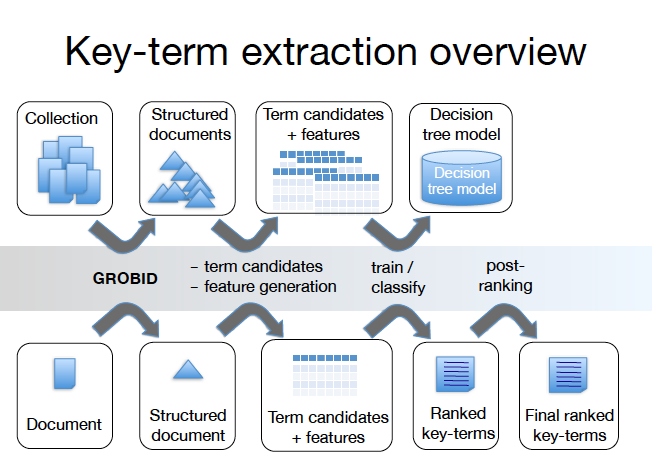
\includegraphics[width=15cm]{img/GROBID/key_term_extraction_GROBID.png}
    \caption{Extraction des termes clés avec GROBID}
    \end{figure}
    
    À partir d'un document donné, le logiciel repère sa structure, composé dans le cadre des articles scientifiques d'un \textit{header}, soit le titre et un résumé, du corps du texte, soit une introduction, des sections et une conclusion, puis d'une liste de références, avec des articles, des revues et des livres, entre autres. GROBID se concentre ensuite sur les termes équivalents et les \textit{features}, soit la présence de références bibliographiques dans le \textit{header} et le corps du texte, ainsi que la position de la première occurrence d'un mot dans le document\footcite[p. 15]{GROBID_Publi_Sc}. Il s'agit enfin, en s'inspirant d'un arbre de décision, comme nous l'avons établi dans le cadre de l'encodage des notices de livres d'heures, d'entraîner la classification et la typologie des termes clés. 
	
	GROBID-dictionaries consiste donc à transposer le principe de GROBID aux informations lexicales via une librairie java d'apprentissage supervisé\footnote{L'installation de GROBID-dictionaries se fait à partir du terminal. Cf.\footcite[p. 14]{Grobid_catalogues}.}. Le logiciel GROBID-dictionaries permet alors de traiter, d'extraire des informations textuelles de dictionnaires numérisés enregistrés au format PDF, et de structurer automatiquement les informations en XML-TEI\footcite[p. 34]{encoder_auto_catalogue}. L'intérêt de ce logiciel est de s'adapter aux entrées lexicales par l'apprentissage supervisé, et donc de pouvoir traiter toute ressource numérisée prenant une forme encyclopédique. Pour obtenir l'encodage de sortie souhaité, il faut donc entraîner le modèle selon une structure bien définie des entrées de catalogue. Un fichier XML respectant les standards de la TEI sert donc d'entraînement pour améliorer la performance du logiciel d'apprentissage machine, ce qui signifie que le fichier d'entraînement doit être encodé avec soin manuellement\footcite[p. 39]{encoder_auto_catalogue}. 
	
	Si l'on fait une analogie avec le catalogue de notices de Leroquais, les documents nécessaires à l'apprentissage machine seraient donc d'une part l'établissement des trois notices modèles en XML TEI, d'autre part un fichier .rawtxt qui contiendrait le texte extrait du document source à encoder, soit les notices océrisées. Pour adapter le modèle au cas des notices de livres d'heures, plusieurs niveaux d'entraînement seraient envisageables. Le premier consisterait à établir une segmentation bien précise de l'ensemble du document à encoder, de la structure de la page à l'entrée lexicale. Cela impliquerait de prendre en compte la variété des pages, car une notice peut s'étaler sur plusieurs pages comme recouvrir moins d'une page entière. L'objectif de cette première étape est de séparer le corps du texte des éléments annexes, comme les réclames ou les numéros de page\footcite[p. 21-22]{Grobid_catalogues}. Par lignes de commandes, on crée ensuite les données d'entraînement à partir de données annotées\footcite[p. 23-25]{Grobid_catalogues}. 

Après avoir segmenté la structure générale de la page, la deuxième étape se concentre sur la segmentation du corps du texte, soit dans notre cas les différentes parties constitutives de la notice, celles qui apparaissent systématiquement (le numéro et le titre de la notice, le résumé et le détail du contenu, les éléments concernant la reliure, etc.), comme celles qui n'apparaissent pas à chaque fois (l'historique ou les références bibliographiques par exemple). De même, les données d'entraînement sont créées et annotées. 

Enfin, pour l'analyse des dictionnaires, les troisième et quatrième niveaux d'entraînement s'appuient sur les entrées lexicales, leurs formes et leurs sens. Si l'on adapte le modèle aux notices de livres d'heures, il faudrait créer et annoter autant de données d'entraînement que de balises TEI définies dans le format cible, afin que le modèle reconnaisse ce qui concerne le \textless msContents\textgreater, le \textless physDesc\textgreater, l'\textless history\textgreater~ ou l'\textless additional\textgreater~.
	
	Toutefois, l'expérience de l'encodage automatisé des catalogues de ventes montre que l'apprentissage machine n'est pas une science exacte. Malgré la quantité et la qualité des données, les résultats d'encodage n'ont pas toujours été pertinents. Pour améliorer les résultats, il a été fait appel au \textit{feature engineering}. Le \textit{feature} renvoie à une représentation numérique d'un aspect de la donnée brute, préparée pour l'algorithme, afin de servir d'intermédiaire entre celles-ci et les modèles utilisés. Le \textit{feature engineering} consiste donc à déterminer quels sont le ou les \textit{features} les plus pertinents à extraire des données brutes disponibles pour arriver aux meilleurs résultats. Cette technique doit être contextuelle pour être efficace, dépendant à la fois des données à traiter, du modèle d'apprentissage utilisé et de l'objectif final. Dans cette exemple, le \textit{feature engineering} s'est traduit par le remplacement d’un modèle unigramme par un modèle bigramme, appliqué aux mêmes données d’entraînement et d’évaluation. Un modèle unigramme associe une étiquette à une unité lexicale fournie en fonction des seules caractéristiques de cet élément. Un modèle bigramme prend lui en compte l’étiquette appliquée à l'unité lexicale précédente pour améliorer l’exactitude de l’étiquetage. Cette étape a considérablement amélioré le modèle dans le cas des catalogues de ventes d'autographes\footcite[p. 42-44]{encoder_auto_catalogue}. \\
	
	\textit{In fine}, la technologie développée par le logiciel GROBID s'appuie sur les éléments de mise en page, le texte et la ponctuation, ce qui signifie que la qualité de l'océrisation est cruciale\footcite[p. 59]{Grobid_catalogues}, mais cette remarque vaut pour tout processus d'encodage que l'on souhaite automatiser. Par ailleurs, plus la structure du document cible est complexe (enchaînement et imbrication des balises TEI), plus l'entraînement et l'apprentissage du modèle seront longs et complexes. Mettre au point une automatisation de l'encodage des notices de livres d'heures établies par Victor Leroquais demanderait donc du temps, ainsi que les moyens financiers et humains adéquats pour trouver des solutions le plus rapidement et efficacement possible. Si l'aventure peut s'avérer complexe et ardue, la création d'un logiciel d'encodage automatique de catalogues de notices de manuscrits, s'appuyant sur des modèles d'encodage en XML TEI défini en amont, pourrait par la suite représenter un gain de temps considérable, bien que la vérification de l'intégrité des données et les éventuelles corrections manuelles restent essentielles pour s'assurer de la qualité des données. \\
	
	Si la structuration de catalogues de notices peut se faire au format XML TEI, structurer des données en masse complexes et liées entre elles implique d’utiliser une base de données relationnelles. 

	
	\chapter{\label{modelisation}De l’importance de la modélisation des données}
	
	La modélisation, opération qui consiste à schématiser un modèle complexe afin de mieux \og mesurer les effets sur ce système des variations de tel ou tel de ses éléments composants\fg{}\footnote{Cf. \url{https://www.cnrtl.fr/definition/modélisation}.}, est une étape essentielle à tout import de données dans une base appropriée. En effet, elle permet de structurer les données, d'établir leurs relations et la cardinalité de leurs relations, c'est-à-dire le nombre d'occurrences minimal et maximal d'une association par rapport à chaque occurrence d'une entité. Pour le projet HORAE, il s'agit de modéliser les usages liturgiques, qui désignent les éléments liturgiques propres à un lieu. Ils peuvent donc être aussi variés que le kaléidoscope de livres d'heures conservés.

	\section{Modéliser les usages : restituer une réalité complexe }
	
	Modéliser, c'est d'abord comprendre ce que l'on doit représenter, les données qui sont à manipuler. On peut alors dresser un modèle conceptuel qui définit les données, leur mode d'évolution dans le temps et leurs relations. La deuxième étape consiste à le transformer en un modèle logique relationnel pour que les données deviennent des objets manipulables dans la base de données relationnelle. Enfin, des tests pour l'implémentation dans la base ont été effectués, afin de définir quelle est la solution la plus intéressante intellectutellement, applicativement et ergonomiquement pour l'import des données.
	
	\subsection{Qu’est-ce que l'usage liturgique ?}
	
	Si le cursus correspond aux chants, lectures et oraisons choisis par une communauté religieuse pour célébrer les offices et la messe des fêtes du sanctoral et du temporal, ces différentes manières de célébrer le culte dépendent de ce que l'on appelle l'usage liturgique. Ce terme désigne l’ensemble des pratiques particulières au culte d’une communauté, relative à un chapitre, une abbaye, un diocèse ou un ordre religieux. De fait, la mention du cursus d'un lieu sert à évoquer les choix de pièces qui caractérisent les heures de la Vierge à l'usage de ce lieu, par exemple. Si l'usage ne modifie pas la structure même de l'office\footnote{L'office désigne un ensemble de lectures et de prières prévues pour un moment précis.} et de la messe\footnote{Célébration collective de l'office du jour.}, il se distingue par\footcite{usages_lit} : 
	\begin{itemize}
	    \item le culte rendu à des saints particuliers ;
	    \item la préséance entre les offices\footnote{L'une des principales difficultés dans la récitation de l’office des heures et la célébration de la messe provient de la superposition du temporal et du sanctoral, c’est-à-dire lorsqu’une ou plusieurs célébrations issues du temps de l'année liturgique ou de celui des saints se superposent le même jour. Ces cas sont résolus grâce à l’établissement de préséances entre les divers offices, susceptibles toutefois de présenter de nombreuses variantes selon les usages. Cf. \cite{preseance_offices}.} ;
	    \item le choix ou la création de pièces liturgiques dans les propres du temps et des saints ;
	    \item des cérémonies particulières, comme des processions.
	\end{itemize}
	
	Dans le cadre du projet HORAE, il s'agit de déceler les dévotions les plus intimes à partir des usages présents dans les livres d'heures. On peut caractériser ces usages grâce à plusieurs critères, en premier lieu la rubrique. Si ces mentions deviennent plus fréquente à la fin du Moyen Âge, il convient de les regarder avec un œil critique. L'usage inscrit n'est en effet pas toujours celui de la destination liturgique. Ainsi, dans les livres d’heures, les usages de l’office des morts ou du petit office de la Vierge les plus répandus sont ceux de Rome, Paris, Sarum\footnote{Aussi appelé usage de Salisbury, c'est une synthèse des usages en vogue en Grande-Bretagne et du rite pratiqué à Rouen.} et Utrecht. Ils n'indiquent pas pour autant de manière systématique la destination du manuscrit\footcite{usages_lit}. 
	
	Un autre critère est celui des calendriers. On peut en effet y trouver les fêtes des saints locaux, mais aussi la fête d'anniversaire de la dédicace de l'église locale et la fête de ses reliques ; la mention d'obits\footnote{Un obit est une messe célébrée par fondation pour un défunt à la date anniversaire de son décès.} et de fondations, bien qu'il faille distinguer  celles dues à la copie primitive et celles ajoutées ultérieurement ; le rite des offices, ou encore les jeux d'encre mettant en valeur telle ou telle fête. Toutefois, l'examen du calendrier doit être mis en regard avec le contenu du manuscrit qui confirme ou infirme l'usage qui ressort du calendrier\footcite{usages_lit}.
	
	Un autre pan du livre d'heures intéressant à observer pour caractériser les usages sont les litanies. Il s'agit d'une liste de saints invoqués. On prête alors particulièrement attention aux saints locaux, mais aussi à la catégorie dans laquelle ils se trouvent (martyrs, apôtres ou confesseurs)\footcite{usages_lit}. 
	
	Les autres éléments révélateurs sont les propres du sanctoral\footnote{Il s'agit de l'ensemble des fêtes des saints du calendrier liturgique célébrées.}, les messes et offices votifs, parfois liés à des reliques locales ou les précisions toponymiques pour les processions\footcite{usages_lit}. \\
	
	Toutefois, il faut distinguer l'usage et la destination, d'autant plus dans les livres dédiés à la dévotion privée. En effet, le destinataire peut vouloir s'inspirer d'un usage qui n'est pas propre à son lieu de vie. Ainsi, le choix et l'ordre des chants dans le petit office de la Vierge et l'office des morts est propre à un diocèse, à un ordre monastique ou religieux, voire à une abbaye ou à une collégiale, mais l'usage employé ne révèle pas une indication d'origine. Les usages de Rome et de Paris sont par exemple trop répandus pour indiquer une provenance stricte de Paris ou de Rome. C'est pourquoi, dans l'étude des livres d'heures, il est préférable d'employer l'expression \og selon l'usage de\fg{}, à moins que le manuscrit ne fournisse la preuve explicite de sa destination à tel lieu, ordre ou institution\footcite[p. 5]{initiation_man_lit}.\\
	
	Une fois que l'on a saisi ce qu'il faut modéliser, il s'agit de s'interroger sur comment décrire un usage dans une base de données. Lorsqu'il s'agit du cursus, il faut penser simultanément la modélisation de la hiérarchie des objets et de leur ordre de succession, qui constituent deux informations spécifiques à l’usage liturgique. La base de données doit donc répondre à la question suivante : Qu’est-ce qu'une pièce textuelle du livre d’heures, dans sa forme, son contenu et sa place au sein des autres textes, nous dit des usages liturgiques propres à une institution ? \\
	
	Voici notre premier essai de modèle conceptuel\footnote{Une reproduction est disponible en annexes section \ref{doc_modelisation}.} : 
	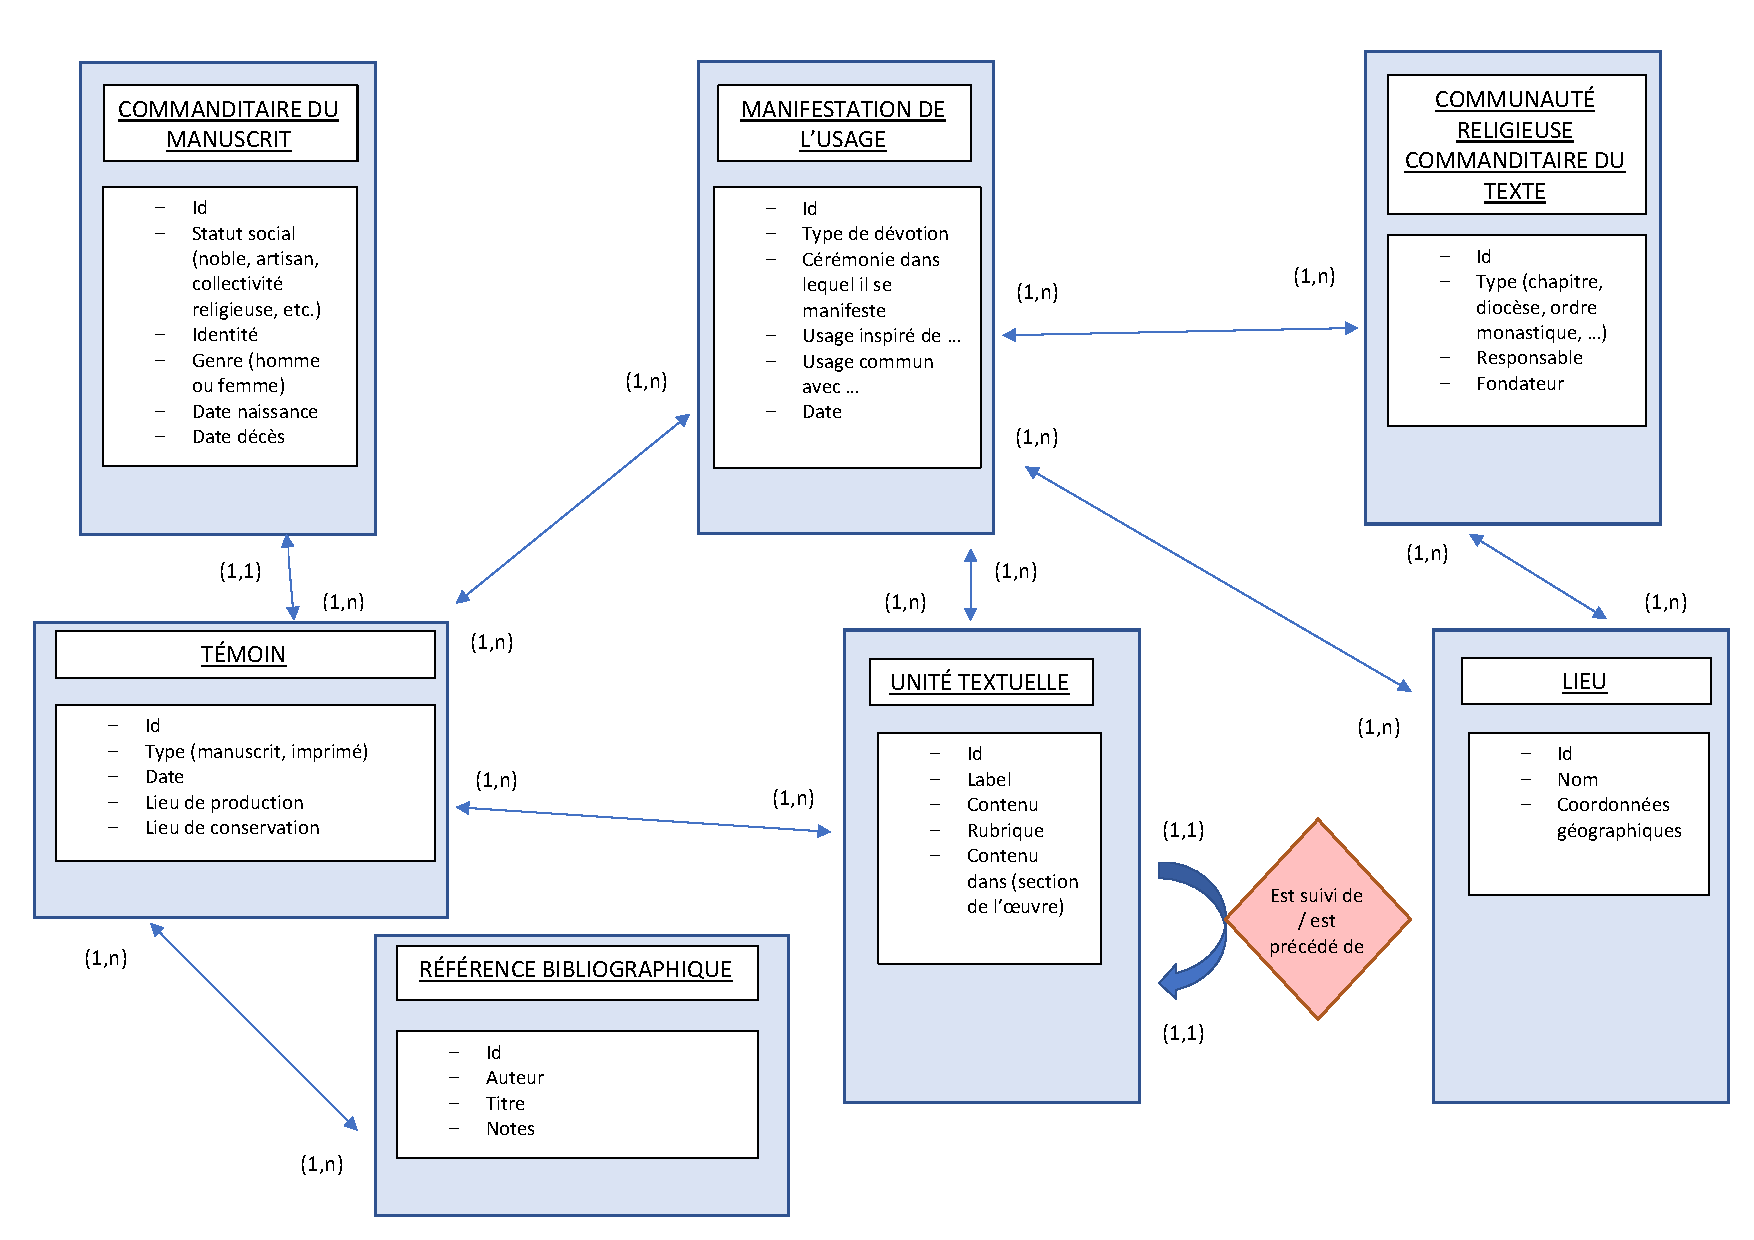
\includepdf[landscape]{img/Modelisation/modelisation1.pdf}
	
	Chaque rectangle correspond à une entité, qui peut contenir plusieurs attributs, ici signalés par des tirets. Il est évident que les attributs sont amenés à être enrichis, et qu'ils ne peuvent être systématiquement renseignés ; tout dépend des données disponibles. Chaque entité possède un identifiant, afin d'être plus facilement manipulable. 
	
	Une bonne modélisation doit respecter un certain nombre de règles de normalisation. Ces règles permettent d'éviter d'éventuels problèmes de transaction, la redondance ou l'incohérence des données, ainsi que des contre-performances. Il faut par exemple éviter d'avoir des attributs calculables à partir d'autres, afin de faciliter les mises à jour des données. Les chiffres entre parenthèses de part et d'autre des flèches, qui par ailleurs indiquent une relation entre deux entités, correspondent aux cardinalités. Elles se lisent de la manière suivante : un usage liturgique se manifeste dans une à plusieurs unités textuelles, et une unité textuelle appartient à un ou plusieurs usages. Pour répondre à l'exigence de succession et de hiérarchisation des unités textuelles, nous avons eu l'idée de créer un attribut \og contenu dans\fg{} et une relation unaire, c'est-à-dire qu'une unité textuelle peut être précédée et suivie d'autre unités textuelles. Les cardinalités sont cruciales pour établir le modèle logique, qui prend la forme suivante\footnote{Une reproduction de ce modèle est disponible en annexes section \ref{doc_modelisation}.} : 

    \begin{figure}[!h]
    \centering
    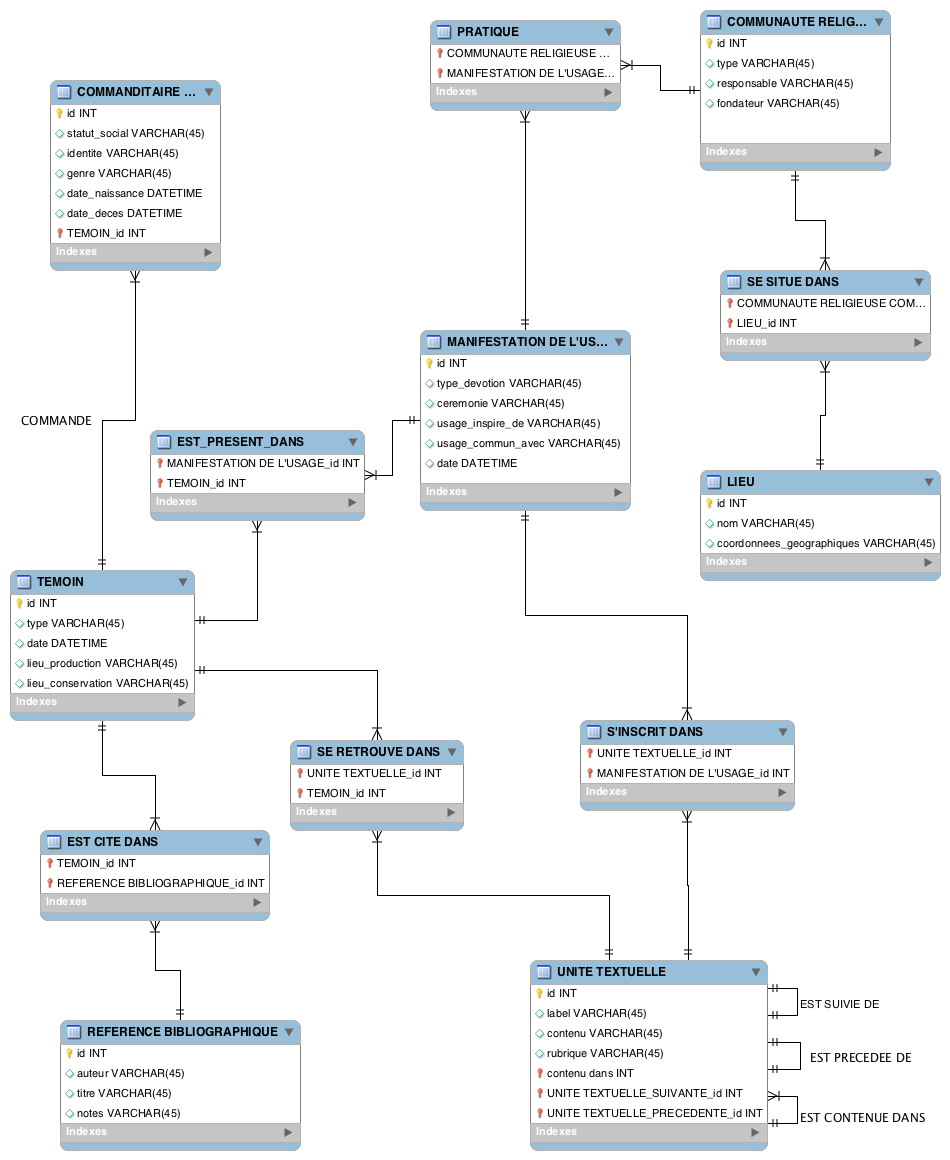
\includegraphics[width=15cm]{img/Modelisation/MRD_Usages.png}
    \caption{Modèle relationnel logique des usages dans les livres d'heures}
    \end{figure}
    \clearpage
	
	En fait, il s'agit de prendre les deux occurrences les plus grandes des couples de cardinalités. Si les deux correspondent à \og n\fg{} occurrences, alors une table de relation est créée, prenant comme attribut les identifiants des entités qu'elle relie, identifiants qui deviennent alors des clés étrangères\footnote{Dans une base de données, une clé étrangère permet de référencer le champ d'une autre table en le désignant par son identifiant.}. On peut donc lire le modèle de la manière suivante : un usage est présent dans un ou plusieurs témoins. Une communauté religieuse pratique un ou plusieurs usages. Une unité textuelle s'inscrit dans un ou plusieurs usages. Une communauté religieuse se situe dans un ou plusieurs lieux. Une personne commande un à plusieurs manuscrit(s). Un témoin est cité dans une ou plusieurs référence(s) bibliographique(s). Une unité textuelle se retrouve dans un à plusieurs témoins. Une unité textuelle est suivie, précédée et contenue dans une autre unité textuelle, sachant que ces trois relations de succession et d'imbrication sont manifestées par des clés étrangères. Toutefois, ce modèle présente quelques défauts. Par exemple, les attributs de lieux de production et de conservation au sein de l’entité \og Témoin\fg{} peuvent être modifiés en des associations vers l’entité \og Lieu\fg{}.\\
	
	Quatre tests ont ensuite été effectués quant à l'implémentation des unités textuelles dans la base Heurist. Heurist, base de données opensource MySQL, a justement été pensée pour les données de recherche en sciences humaines et sociales, qui se caractérisent par leur richesse, leur hétérogénéité, leur imperfection et leur forte interconnexion. Ainsi, tout système d’information pour un projet en humanités numériques doit permettre des requêtes complexes, un rendu de résultats interactifs et éditables, un export de données en divers formats, une certaine durabilité, et éventuellement un modèle pour le travail en groupe et parfois la publication sélective de données sur le web\footcite{bd_Heurist}. La base est déployée sur les serveurs de la TGIR Humanum, infrastructure de recherche pour les humanités numériques à l'échelle nationale et internationale\footnote{Cf. \url{https://www.huma-num.fr/}.}. 
	
	Les quatre tests présentés ci-dessous visent donc à visualiser la solution la plus pertinente pour rendre compte de ce qui fait toute la complexité et la richesse des livres d'heures : le double processus de succession pour les sections et les pièces, ainsi que d'imbrication des pièces liturgiques dans les sections, l'ensemble correspondant à un usage bien précis. 
	
	Dans le premier test, le champ \og UseItem\fg{} revient à une liste sur le séquençage des pièces. Plus on clique sur le lien \og UseItem\fg{}, plus l’arborescence du livre se déploie, jusqu’à arriver au niveau de granularité le plus fin. On peut donc rajouter autant de \og UseItem\fg{} que l’on souhaite. S’il est spécifique à la relation créée, les œuvres restent génériques.
	
    \begin{figure}[!h]
    \centering
    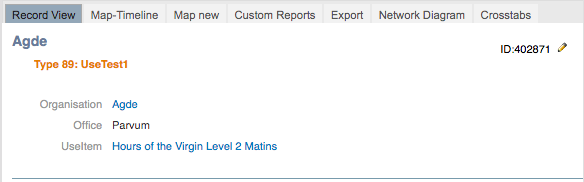
\includegraphics[width=15cm]{img/Modelisation/Tests_Implementation/UseTest1.png}
    \caption{Test d'implémentation n°1}
    \end{figure}
	
 Toutefois, cela n’est pas optimal du point de vue de l’ergonomie. La solution est en effet pratique pour enregistrer la séquence, mais si l’on supprime un \og UseItem\fg{}, les autres pièces qu'il contient sont supprimées. \\
 
 La solution du deuxième test permet de visualiser, par l'intermédiaire de relations, la succession des sections au sein de l’ouvrage, jusqu’à avoir accès au texte pour la plus fine granularité, soit la dernière relation présentée ci-dessous. 
 
    \begin{figure}[!h]
    \centering
    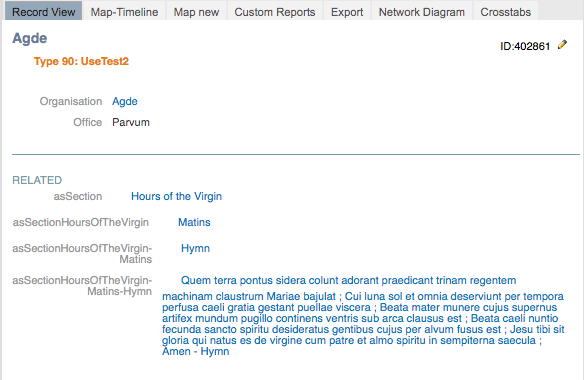
\includegraphics[width=15cm]{img/Modelisation/Tests_Implementation/UseTest2.png}
    \caption{Test d'implémentation n°2}
    \end{figure}
 
 Cette idée est visuellement intéressante mais pas suffisamment pertinente du point de vue des imbrications dans les noms donnés aux relations, car plus la granularité est fine, plus les noms des relations s'allongent. Pour des questions d'intéropérabilité, il est en effet souhaitable d'utiliser le vocabulaire implémenté dans Heurist pour typer les relations. Dans le cas des pièces liturgiques, il est préférable d'utiliser celui de la \og séquence\fg{} dans la section \og temporal\fg{}, soit les termes suivants :
 \begin{itemize}
     \item EndsBefore ;
     \item ImmediatelyFollows ;
     \item ImmediatelyPrecedes ;
     \item StartsAfter.
 \end{itemize} 
En outre, la linéarité ne modélise pas la séquence. Ceci pose le problème de la modélisation appliquée à un logiciel. Si une information n’est pas modifiable dans le logiciel, c'est que le problème vient du modèle sous-jacent qui doit être compatible avec le logiciel utilisé.\\

La troisième implémentation rend davantage compte de la réalité du texte dans l’usage. 

    \begin{figure}[!h]
    \centering
    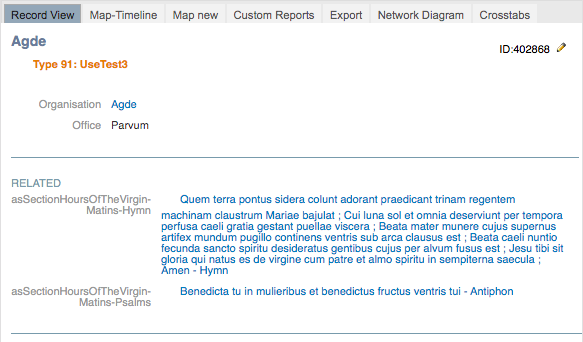
\includegraphics[width=15cm]{img/Modelisation/Tests_Implementation/UseTest3.png}
    \caption{Test d'implémentation n°3}
    \end{figure}

Si la relation vers la section apparaît, ce n'est pas le cas de la hiérarchie des textes.\\

La solution la plus satisfaisante est la quatrième. Visuellement le texte apparaît comme dans la source. Si l’on clique dessus, on voit le texte comme une entité avec ses relations aux autres sections, à l'image du deuxième test.

    \begin{figure}[!h]
    \centering
    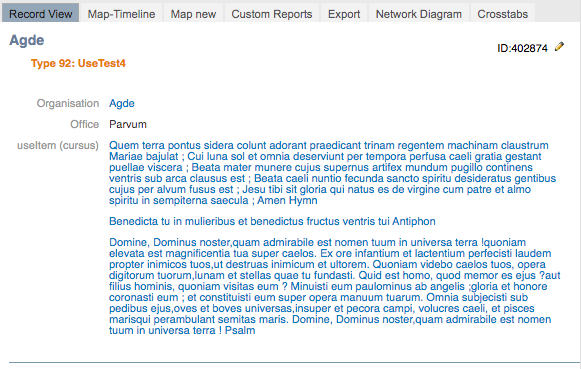
\includegraphics[width=15cm]{img/Modelisation/Tests_Implementation/UseTest4.png}
    \caption{Test d'implémentation n°4}
    \end{figure}

Ce modèle est d'un point de vue intellectuel et applicatif supérieur, car l'on se rapproche du modèle RDF où chaque relation n'est déclarée qu’une seule fois, et donc la hiérarchie une seule fois également\footnote{L'inspiration du modèle RDF pour cette implémentation est explicitée à la sous-partie \ref{modeles_standards}.}. Cependant, il peut être plus pertinent de typer la relation par \og ImmediatelyFollows\fg{}, en partant de l’entité vers l'entité précédente, car dans notre lecture du livre de gauche à droite, on est sûr de ce qui précède mais pas de ce qui suit. 

Toutefois, il faudrait ajouter le séquençage des sections en plus de l’ordre affiché au sein des œuvres. Le problème est en effet de représenter à la fois la succession au niveau des pièces et la succession au niveau des sections. Cette dernière idée s’implémente ainsi dans la description de l’usage : 
\begin{quote}
Agde(use) :contains :Matins, Agde(use) :contains :Lauds, :contains(1) :precedes :contains(2)
\end{quote}

Se pose également la question des usages pour les pièces non-renseignées, ou bien si la source utilisée ne contient pas l’information mais que cette dernière est peut-être présente dans d’autres témoins. Les pièces absentes ou inconnues révèlent en effet la nécessité de choisir un format qui est facile à générer si on met à jour le cursus et qu’on trouve une pièce non-renseignée. 

Ainsi, chercher l'inspiration du côté de standards utilisés dans les notices bibliographiques ou pour le web sémantique aide à penser la modélisation et les possibles implémentations du modèle dans la base.

	
	\subsection{\label{modeles_standards}S’inspirer de modèles standardisés}
	
	Différents modèles peuvent nous aider à modéliser le cursus. Une des premières sources d'inspiration à laquelle on peut se référer est la modélisation de la séquence par Georg Vogeler. Historien au centre de modélisation de l'information en Humanités à l'Université de Graz, Georg Vogeler mène des recherches en technologies numériques pour les sciences sociales, les arts, les humanités, la structuration des données et l'histoire culturelle. Sa proposition prend la forme suivante :
	
	\begin{quote}
:S1 a :Sequence ; :hasStart :Hour1; :hasEnd :Hour2; :isDocumentedIn :BookOfHoursX .
:text a rdf:List; :isDocumentedIn :Book1; rdf:first :fragment1 .
:fragment1 :references :Hour1; rdf:rest _:tf1 . _t:ft1 rdf:first :fragment2; :references :Hour2, rdf:rest rdf:nil .
:Book1 :contains :fragment1, :fragment2 . :fragment2 :follows :fragment1 . :fragment1 :references :Hour1 . :fragment2 :references :Hour2 .
	\end{quote}
	
	Ce modèle s'appuie sur un standard propre au web sémantique : le triplet RDF. Le web sémantique est en fait une extension du web courant qui vise à donner du sens au contenu des pages web, en majorité créées pour être lues, et permettre leur interprétation par des machines. Un standard comme RDF\footnote{\textit{Ressource Description Framework}.}, doté d'un vocabulaire spécifié par le W3C\footnote{\textit{World Wide Web Consortium}. Organisme de standardisation fondé en 1994, il a pour but de favoriser la compatibilité des différentes technologies du Web.}, sert à attribuer un sens défini à chaque donnée, à créer un réseau d'informations structurées facilement réutilisables. Il s'agit alors d'éviter les redondances, les conversions lourdes, et de permettre la traçabilité des données\footnote{Cf. \url{https://www.enssib.fr/le-dictionnaire/web-semantique}.}. 
	
	La modélisation de la séquence de Georg Vogeler s'inspire du modèle RDF car on retrouve bien la structure en triplet séparée par des points-virgules. L'information est ainsi formée :
	\begin{itemize}
	    \item d'un sujet
	    \item d'un prédicat
	    \item d'un objet
	\end{itemize}
	Les sujets sont ici en début de ligne : \og S1\fg{} fait référence à un sujet lambda que l'on pourrait retrouver dans le cadre des livres d'heures, tout comme \og text\fg{}, \og fragment1\fg{} et \og Book1\fg{}. Les prédicats se trouvent en deuxième position : \og a\fg{} correspond à \og rdf:type\fg{} et révèle donc la nature du sujet ; les autres prédicats, aisément compréhensibles, indiquent des relations de succession, de hiérarchie, de contenu et de contenant (\og hasStart\fg{} ; \og hasEnd\fg{} ; \og isDocumentedIn\fg{} ; \og references\fg{} ; \og contains\fg{} ; \og follows\fg{}). L'appellation \og rdf:first\fg{} indique le premier type d'occurrence dans un sujet de type liste, tandis que le prédicat \og rdf:rest\fg{} signale le reste des autres éléments d'une liste\footnote{Cf. \url{https://www.w3.org/TR/rdf-schema/#ch_first}.}. Quant aux objets, ils sont ici propres à la modélisation de la séquence du cursus, formés d'une suite de sections et de pièces liturgiques à l'intérieur d'un livre d'heures qui s'interpénètrent entre elles. 
	
	Si l'on adapte cette proposition à une base de données relationnelle, car les données du projet sont ici destinées à être structurées dans la base Heurist et non sur le web sémantique, les sujets et objets des triplets peuvent faire référence à des clés étrangères. On peut également typer les relations avec un vocabulaire spécifique pour préciser où l’on se trouve dans le cursus. C'est justement l'association spécifique entre un usage et une œuvre que l'on nomme cursus.\\
	
	Il est intéressant pour notre réflexion de croiser ce type de modèle avec le standard FRBR\footnote{\textit{Functional Requirements for Bibliographic Records}.}. Il s’agit d’une modélisation conceptuelle de l'information contenue dans les notices bibliographiques. Élaborée en 1997, cette modélisation est née de l'informatisation des données bibliographiques depuis les années 1970. Des programmes de catalogues partagés ont alors vu le jour. Outil de description, un catalogue sert à localiser physiquement des supports de contenus. L’unité d’information primordiale est donc le support. Ainsi, lorsque l’on cherche une œuvre, celle-ci n’apparaît pas comme une unité intellectuelle, mais sous la forme d’une liste des différentes versions de l’œuvre, chaque version ayant sa propre notice distincte dans le catalogue. La particularité du modèle FRBR est d'inverser cette approche : l’œuvre devient le concept central. Les œuvres sont ensuite déclinées en manifestations, qui peuvent recouvrir divers supports comme divers langages. Le but est de créer une notice unique par œuvre qui permet d’accéder à toutes les versions, linguistiques comme d'édition, et à tous les supports de l’œuvre et de ses adaptations, du livre au livre audio en passant par le DVD, par exemple\footnote{Cf. \url{https://www.enssib.fr/bibliotheque-numerique/documents/65520-comprendre-le-modele-frbr-et-ses-extensions.pdf}.}. En voici une schématisation\footnote{Le schéma est extrait du site suivante : \url{https://fr.slideshare.net/nonue12/crfcb-amu-evolutionscatalogage091213-frbr}.} : 
	
	\begin{figure}[!h]
    \centering
    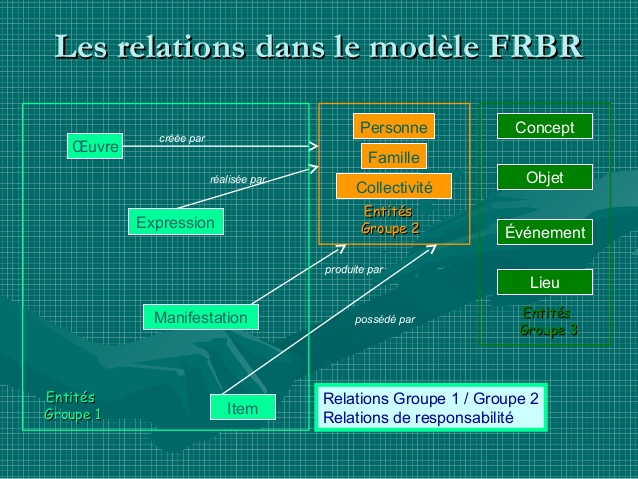
\includegraphics[width=15cm]{img/Modelisation/Modele_type_FRBR.jpg}
    \caption{Modélisation conceptuelle des usages dans les livres d'heures inspirée du modèle FRBR}
    \end{figure}
    \clearpage
    
    L'entité \og Œuvre\fg{} se réfère aux caractéristiques de la création abstraite à laquelle se rattache son contenu. L'\og Expression\fg{} indique les caractéristiques de son contenu intellectuel ou artistique, la \og Manifestation\fg{} les caractéristiques de la publication à laquelle elle appartient, et enfin l'\og Item\fg{} ses caractéristiques individuelles en tant qu’exemplaire. On va donc dans la caractérisation de l'œuvre du plus abstrait au plus concret. Ces niveaux d'analyse du document décrit peuvent être mis en relation avec des entités qui sont intervenues dans le processus de création ou de production, mais aussi avec des notions constituant les sujets inhérents à l'œuvre\footnote{Cf. \url{https://www.bnf.fr/fr/modeles-frbr-frad-et-frsad}.}. 
   
    Voici une nouvelle modélisation, inspirée à la fois des triplets RDF et du modèle FRBR, adpatée au cas du cursus et des usages résultant de l'analyse des livres d'heures\footnote{Une reproduction de ce modèle est disponible en annexes section \ref{doc_modelisation}.} : 
    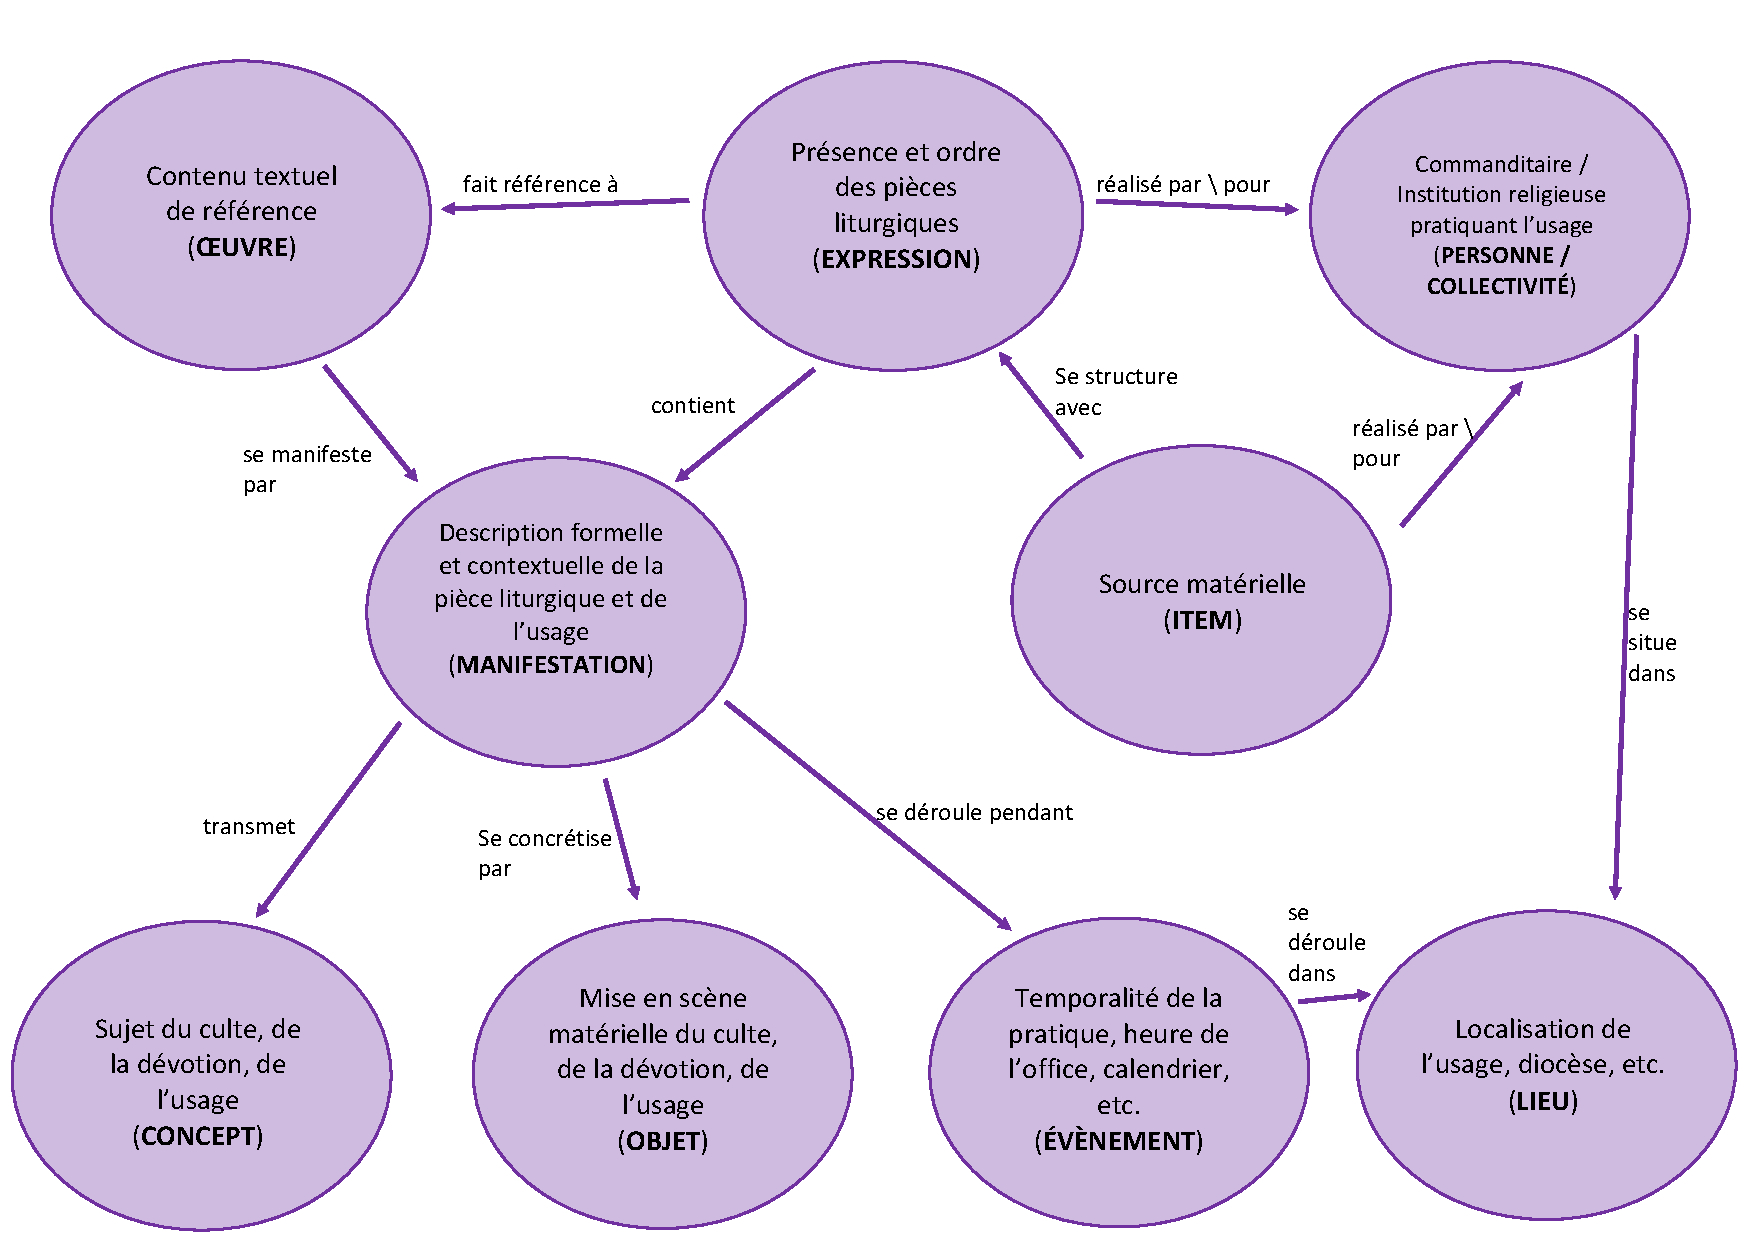
\includepdf[landscape]{img/Modelisation/Modelisation_RDF_FRBR.pdf}
    
    Le modèle tend à rendre compte que, par exemple, les matines de l'usage d'Agde sont une expression de l'œuvre que constitue les matines, et donc que l'expression d'une même œuvre diffère selon les usages. S'inspirer de standards de modélisation propres au monde du web sémantique ou de la bibliothéconomie aide à enrichir la réflexion, mais il est évident que le modèle exposé ci-dessus ne peut être implémenté tel quel dans la base de données relationnelles. On peut ainsi reprocher à ce modèle d'être restrictif dans les types de relations, qui ne sont pas nécessairement à sens unique entre les entités, mais soulève également quelques problèmes : l'\og Œuvre\fg{} est-elle réellement détachable du \og Concept\fg{} ? L'\og Item\fg{} et l'\og Objet\fg{} ne peuvent-ils être réunis sous une même entité ? \\
    
    Dans l'optique de l'import des données, c'est la solution suivante qui a été conservée :

    \begin{figure}[!h]
    \centering
    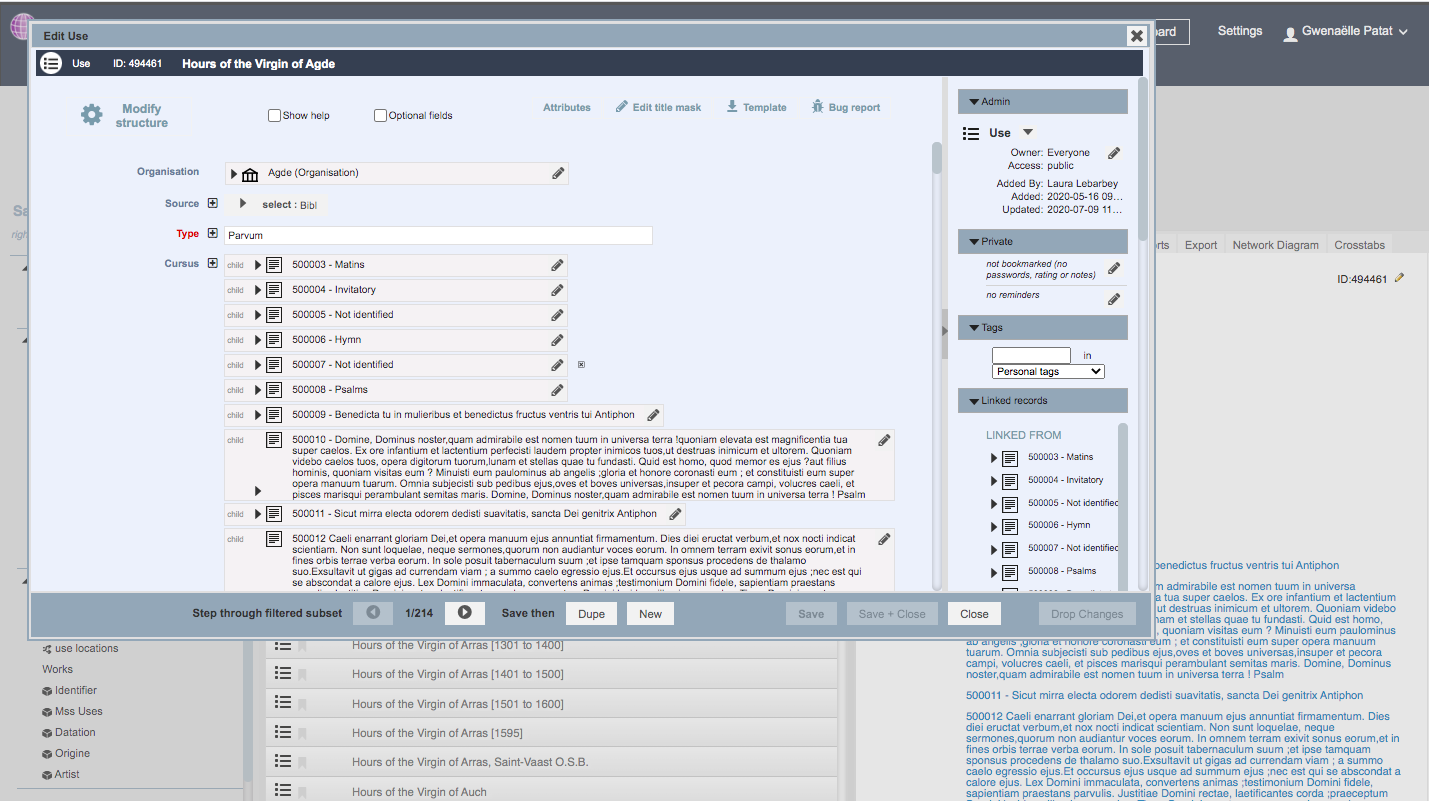
\includegraphics[width=15cm]{img/Modelisation/choix_final_use.png}
    \caption{Modèle d'implémentation de l'entité Use}
    \end{figure}
    
    \begin{figure}[!h]
    \centering
    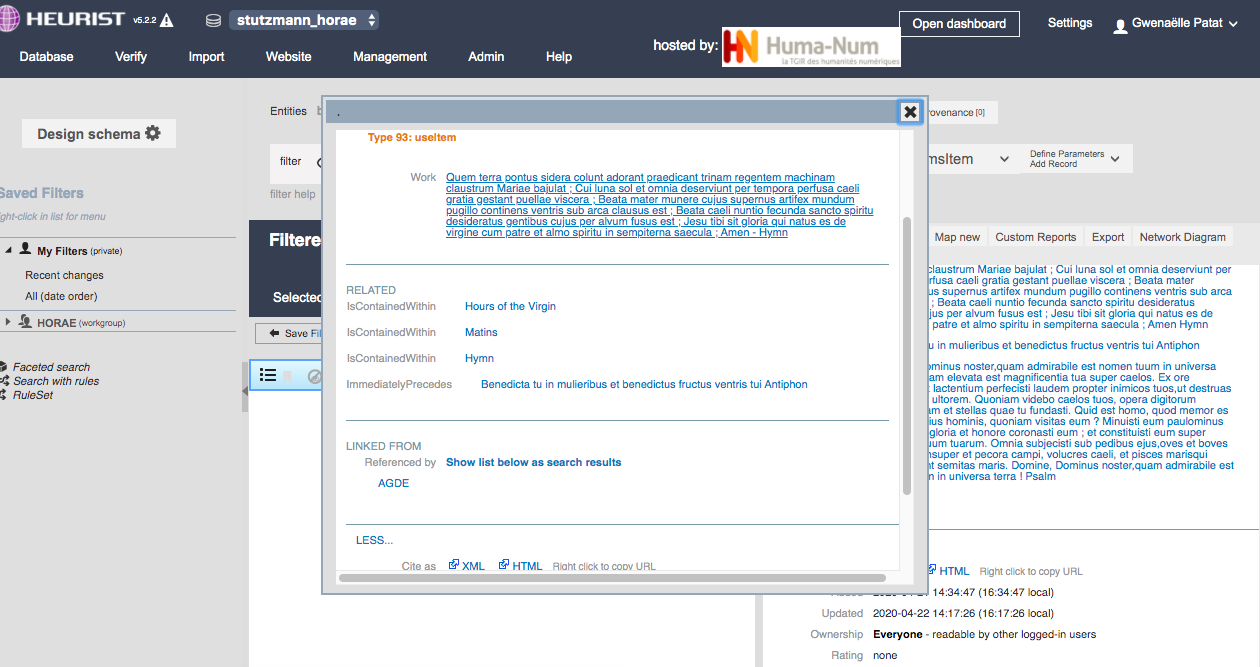
\includegraphics[width=15cm]{img/Modelisation/choix_final_useItem.png}
    \caption{Modèle d'implémentation de l'entité UseItem}
    \end{figure}
    \clearpage
    
    \begin{figure}[!h]
    \centering
    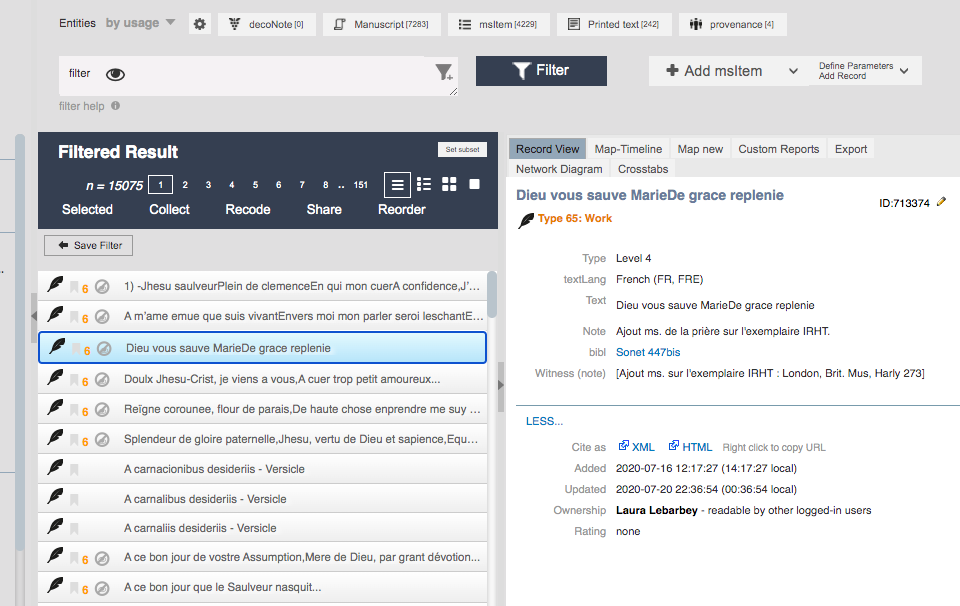
\includegraphics[width=15cm]{img/Modelisation/choix_final_work.png}
    \caption{Modèle d'implémentation de l'entité Work}
    \end{figure}
    
    L'usage (l'entité \og Use\fg{}) a pour attributs :
    \begin{itemize}
        \item l'organisation à laquelle il est relié\footnote{À noter qu'un usage peut être relié à une ou plusieurs organisations.}
        \item les références bibliographiques dans lesquelles il est mentionné ;
        \item son type, \og parvum\fg{} ou \og magnum\fg{}\footnote{On peut aussi créer un \og subtype\fg{} pour déterminer ce qui est de l’ordre du \og Parvum\fg{} ou du \og Magnum\fg{} dans l’usage concerné. En effet, le type d’office ne concerne pas tout le cursus mais une ou des office(s) en particulier.} ;
        \item le cursus, qui est constitué d'une succession de pièces liturgiques, soit l'entité \og useItem\fg{} dans la base.
    \end{itemize}\\
    
    L'entité \og useItem\fg{} est quant à elle dotée de l'attribut \og work\fg{}, qui renvoie au contenu textuel de la pièce, et d'un ensemble de relation de succession (\og ImmeditatelyFollows\fg{} ou \og ImmediatelyPrecedes\fg{}) et de hiérarchie (\og Contains\fg{} ou \og IsContainedWithin\fg{}). Si l'on clique sur l'attribut \og work\fg{} d'un \og useItem\fg{}, s'ouvre la page relative à l'entité \og Work\fg{} dans laquelle on trouve le niveau de granularité du texte, de \og Level 1\fg{} pour les sections les plus englobantes au \og Level 4\fg{} pour le niveau le plus fin. On peut lire ensuite le texte lui-même, ou les sections de texte contenues dans une section englobante, ainsi qu'une éventuelle \og Note\fg{}, la référence bibliographique dans laquelle le texte transmis est transcrit (\og bibl\fg{}), et les témoins dans lesquels on retrouve le texte (\og Witness\fg{}). \\
    
    Comment implémenter les données selon ce modèle dans la base heurist ?
    
    
	\section{L’impossible import des données structurées en xml : bilan d’une tentative avortée et solutions alternatives}
	
	Les données sont stockées dans des tableurs, aux formats excel ou csv\footnote{\textit{Signifiant Comma-Separated Values}, le CSV est un format texte servant à représenter des informations sous forme tabulaire : les sauts de lignes correspondent à des changements de lignes et les virgules (ou points-virgules selon les cas), indiquent la séparation entre les colonnes.}. Les colonnes divisent les informations relatives au cursus, avec le nom de l'usage liturgique, les différents niveaux hiérarchiques et œuvres associées, ainsi que le texte qui le compose. La base Heurist offre plusieurs possibilités d'import, parmi lesquels l'usage de CSV, d'une bibliographie Zotero, d'un document au format KML pour les données géospatiales\footnote{\textit{Keyhole Markup Language}. C'est un langage formé de balises destiné à la gestion de l'affichage de données géospatiales dans les logiciels de Système d'Information Géographique (SIG).}, ou encore aux formats XML ou JSON. Pour l'import du cursus, l'enjeu était de savoir quel import était le plus rapide et le plus pertinent : passer par des données stockées dans un document CSV ou XML ?
	
	\subsection{Définir la structure du format cible en XML}
	
	Avant toute structuration des données pour l'import, il faut savoir quelle forme doit prendre le document d'import, mais aussi s'assurer que les données sont homogènes. Ainsi, quand les données sont divisées en plusieurs csv, il faut pouvoir faire des jointures à partir de données cohérentes. Par exemple, les informations relatives au champs \og Work\fg{}\footnote{Document Export\_stutzmann\_horae\_t65\_Work.csv.}, qui correspond au texte d'une pièce liturgique, étaient dissociées des informations relatives au cursus\footnote{Document Cursus\_HORAE\_Listes\_import\_heurist.xlsx.}. Via le logiciel Dataiku, on peut faire cette jointure grâce à une condition d'égalité entre les colonnes \og function\fg{} dans le document Cursus\_HORAE\_Listes\_import\_heurist.xlsx et \og liturgical function\fg{} dans le document Export\_stutzmann\_horae\_t65\_Work.csv, ainsi qu'une condition de jointure si les colonnes \og Text\fg{} ont les mêmes premiers mots. On obtient alors le tableau avec les colonnes suivantes pour tester la solution d'import des données la plus efficiente\footnote{Il convient de préciser que chaque ligne du tableau correspond à une pièce liturgique précise au sein d'un usage, soit l'entité appelée \og useItem\fg{} au sein de la base.} : 
	\begin{itemize}
	    \item la colonne \og Numérotation\fg{}, soit le numéro de ligne associée à chaque useItem afin de se retrouver dans les données\footnote{Le tableau servant aux tests d'import, UseItem\_Test\_LL.xlsx, contient en effet 4620 entrées.} ;
	    \item \og Use\fg{}, qui correspond à l'usage en vigueur et qui prend le nom de l'organisation à laquelle il est associé ;
	    \item \og Office\fg{}, qui prend la valeur de \og Parvum\fg{} ou \og Magnum\fg{} ;
	    \item Level 1 à 4 qui indiquent les relations de séquence et d'imbrication entre les pièces (\og IsContainedWithin\fg{});
	    \item title level 1 à 4, indiquant les titres des pièces dont il est question, des Heures de la Vierge aux psaumes ou hymnes en passant par les Matines ou Complies ; 
	    \item \og function\fg{}, correspondant à la fonction liturgique, de l'invitatoire au versicule en passant par l'hymne ou le répons ;
	    \item \og Text\fg{} pour le texte associé à la pièce ;
	    \item H-ID Work 1 à 4, soit les identifiants générés par Heurist pour les entités existantes dans la base ;
	    \item ID HORAE 1 à 4, les identifiants choisis par l'administrateur de la base, afin que les relations entre les entités soient faites au moment de l'import même entre les entités qui n'ont pas encore de \textit{record indentifier} générés par la base Heurist ;
	    \item Work title 1 à Work title 4, soit le contenu textuel des œuvres présentes dans l'usage.
	\end{itemize}\\
	
	À terme, les données doivent également être liées à des ressources extérieures, comme les cotes des sources ou les références bibliographiques dans lesquelles elles sont citées et décrites, notamment dans les catalogues de notices\footnote{Ces dernières informations apparaissent dans les colonnes \og Sources manuscrites et imprimées\fg{}, \og Bibliographie\fg{}, \og Remarques\fg{} et \og Reproduction\fg{} du tableau de données \og Cursus\_HORAE\_Listes.xlsx\fg{}.}. \\
	
	Pour tester un import en XML, il a fallu comprendre comment les données à disposition, dans un format csv, allaient être encodées automatiquement dans un format XML, et quelle forme le document d'import allait prendre. Dans un premier temps, nous avons élaboré le document d'import à partir d'un export de données déjà présentes dans la base et concernant le cursus. Le document d'export en XML prend la forme suivante : 
	\begin{minted}{XML}
<?xml version='1.0' encoding='UTF-8'?>
<hml xmlns="http://heuristnetwork.org" xmlns:xsi="http://www.w3.org/2001/
XMLSchema-instance" xsi:schemaLocation="http://heuristnetwork.org/reference/
scheme_hml.xsd">
<database id="0">stutzmann_horae</database>
<query q="t:92" db="stutzmann_horae" depth="all"/>
<dateStamp>2020-04-24T15:24:11+02:00</dateStamp>
<resultCount>1</resultCount>
<records>
<record visibility="viewable" visnote="logged in users" 
selected="no" depth="0">
<id>402874</id>
<type id="92" conceptID="0000-92">Use</type>
<citeAs>https://heurist.huma-num.fr:443/heurist/
?recID=402874&amp;db=stutzmann_horae</citeAs>
<title>Agde (Use) [2]</title>
<added>2020-04-21 16:34:47</added>
<modified>2020-04-24 13:05:03</modified>
<workgroup id="0">public</workgroup>
<raw>2</raw>
<year>2</year>
<detail conceptID="2-21" name="Organisation" 
id="21" basename="Organisation" isRecordPointer=
"true">402689</detail>
<detail conceptID="0000-1011" name="bibl" 
id="1011" basename="bibl" isRecordPointer=
"true">402893</detail>
<detail conceptID="0000-1187" name="Office
" id="1187" basename="Office">Parvum</detail>
<detail conceptID="0000-1191" name="Cursus" 
id="1191" basename="Cursus" isRecordPointer=
"true">402909</detail>
<detail conceptID="0000-1191" name="Cursus" 
id="1191" basename="Cursus" isRecordPointer=
"true">402910</detail>
<detail conceptID="0000-1191" name="Cursus"
id="1191" basename="Cursus" isRecordPointer=
"true">402911</detail>
<detail conceptID="0000-1191" name="Cursus" 
id="1191" basename="Cursus" isRecordPointer=
"true">402875</detail>
<detail conceptID="0000-1191" name="Cursus" 
id="1191" basename="Cursus" isRecordPointer=
"true">402914</detail>
<detail conceptID="0000-1191" name="Cursus" 
id="1191" basename="Cursus" isRecordPointer=
"true">402881</detail>
<detail conceptID="0000-1191" name="Cursus" 
id="1191" basename="Cursus" isRecordPointer=
"true">402887</detail>
</record>
<record visibility="viewable" visnote="logged 
in users" selected="no" depth="1">
<id>402689</id>
<type id="4" conceptID="2-4">Organisation</type>
<citeAs>https://heurist.huma-num.fr:443/heurist/
?recID=402689&amp;db=stutzmann_horae</citeAs>
<title>Agde (Organisation)</title>
<added>2020-04-20 18:15:20</added>
<modified>2020-04-20 18:17:59</modified>
<workgroup id="0">public</workgroup>
<detail conceptID="2-2" name="Short name / 
acronym" id="2" basename="Short name">Agde</detail>
<detail conceptID="2-134" name="Location 
(places)" id="134" basename="Location (place)"
isRecordPointer="true">386187</detail>
<reversePointer id="21" conceptID="2-21" 
basename="Organisation" name="Organisation">
402874</reversePointer>
</record>
[...]
<record visibility="viewable" visnote="logged 
in users" selected="no" depth="1">
<id>402909</id>
<type id="93" conceptID="0000-93">useItem</type>
<citeAs>https://heurist.huma-num.fr:443/heurist/?
recID=402909&amp;db=stutzmann_horae</citeAs>
<title>Hours of the Virgin</title>
<added>2020-04-24 12:38:53</added>
<modified>2020-04-24 12:39:29</modified>
<workgroup id="0">public</workgroup>
<detail conceptID="0000-1134" name="Work" id="1134"
basename="title (work)" isRecordPointer=
"true">75966</detail>
<reversePointer id="1191" conceptID="0000-1191" 
basename="Cursus" name="Cursus">402874</reversePointer>
</record>
	\end{minted}
	
À partir de ce document d'export, où l'on peut voir un enregistrement relatif à l'usage d'Agde, un deuxième à propos de l'organisation d'Agde et un troisième concernant la section \og Hours of the Virgin\fg{}, il est nécessaire de distinguer ce qui est généré par la base de ce qui est à importer et à structurer dans le document d'import en XML. Il est donc important de comprendre à quoi correspond chaque balise et chaque attribut. Si les trois premiers attributs de la balise \textless record\textgreater , qui correspond à un enregistrement, sont propres à l'interface d'Heurist (visibility, visnote, selected), l'attribut \textit{depth} indique le niveau depuis lequel est chargée la donnée, donc il augmente de un dans la relation depuis le document sélectionné, selon le schéma suivant :
\begin{quote}
Agde [usage] (niveau 0, id 402874), Agde [organisation] (niveau 1, id 402689), Agde [place] (niveau 2, id 386187)
Agde [usage] (niveau 0, id 402874), Benedicta tu [useItem] (niveau 1, id 402881), Benedicta tu [work] (niveau 2, id 395935), HORAE [bibl] (niveau 3, id 393553), O quam pulchra (niveau 4, id 399263 = une antienne qui a aussi pour [bibl] = HORAE)   
\end{quote}
La balise \textless id \textgreater~correspond à l'identifiant que l'on veut ici générer automatiquement. La balise \textless type\textgreater~renvoie ensuite au type d'entité, dont les attributs \textit{id} et \textit{conceptId} sont générés par la base. La balise \textless citeAs\textgreater~indique l'URL\footnote{\textit{Uniform Resource Locator}. Une URL est une adresse vers la localisation d'une ressource du web. Elle est notamment constituée du protocole, du nom de domaine et du chemin.} vers la données concernée. La balise \textless title\textgreater~renvoie au titre donné à l'instance de l'entité, tandis que les balises \textless added\textgreater~et \textless modified\textgreater~ sont des informations d'ajout et de modification des données clairement générées par Heurist et que nous n'avons pas à générer nous-même ; \textless workgroup\textgreater~semble également être généré par Heurist et renvoyer à des droits relatifs à la base. Quant aux balises \textless detail\textgreater~et \textless reversePointer\textgreater , elles sont intéressantes pour l'import car permettent de fixer les relations entre les entités. Ces deux dernières balises pointent en effet vers des entités référencées ailleurs dans la base. Ainsi, la balise \textless detail\textgreater~permet de faire des liens entre deux entités, tandis que la relation de séquence et de hiérarchie se fait grâce aux balises \textless detail\textgreater
~des entités de type \og Record relationship\fg{}. Il faut donc générer les clés étrangères au moment des relations. Pour les relations de type \og many to many\fg{} (celles dont le couple de cardinalités est constitué de n,n dans le modèle relationnel logique), elles apparaissent dans les balises \textless detail\textgreater~avec l’attribut IsRecordPointer. Pour une relation \og one to many\fg{} de lien direct (couple de cardinalités 1,n dans le modèle relationnel logique), il faut encoder la balise \textless reversePointer\textgreater. Il faut donc 
être attentif aux identifiants pour créer des relations vers les entités souhaitées, notamment les UseItem au sein du cursus.\\

Dans le document d'export en XML, il nous faut distinguer trois sources différentes dans la structuration de l'information :
\begin{enumerate}
    \item Les données générées par la base Heurist elle-même. S'il est possible de récupérer ces données à partir du document d'export XML, avec des librairies python comme \textit{untangle} pour parser le document, ce qui s'avère inutile car ce sont des informations non nécessaires lors de l'import.
    \item Les données générées automatiquement au moment de d'import, soit les identifiants donnés aux entités, ce qui correspond dans le document d'export XML au texte entre les balises \textless id\textgreater~et \textless detail\textgreater .
    \item Les données générées depuis le(s) fichier(s) csv qui contiennent les données renseignées et homogènes relatives au projet de recherche.
\end{enumerate}
Il est donc nécessaire de comprendre quels sont les identifiants à générer automatiquement et quels sont ceux inhérents à la base de données Heurist. Les relations vers des entités préexistantes dans Heurist, celles qui ont déjà été importées, notamment de type \og Work\fg{} et \og Organisation\fg{}, font donc référence aux identifiants déjà implémentés dans la base et n'ont pas à être générés automatiquement au moment de l'import. De plus, chaque \og useItem\fg{}, que ce soit dans une relation de hiérarchie ou de succession, est spécifique à un usage, donc il est important de tous les différencier selon l’usage auquel ils sont liés. \\

Ce que l'on souhaite importer pour tester l'import, c’est une ou plusieurs instances de type \og Use\fg{}, soit l'usage. L'enregistrement est donc, en général, lié à une entité existante, l'Organisation dans notre cas. L'entité de type \og Use\fg{} est elle-même reliée à une liste d'enregistrements de type \og useItem\fg{}. Les relations entre les \og useItem\fg{} sont implémentées via une table de relation \og Record relationship\fg{}. Le premier document cible pour l'import ressemble donc à ceci : 
\begin{minted}{xml}
<?xml version="1.0" encoding="UTF-8"?>
<hml xmlns="http://heuristnetwork.org" xmlns:xsi="http://www.w3.org/2001
/XMLSchema-instance" xsi:schemaLocation="http://heuristnetwork.org/
reference/scheme_hml.xsd">
    <database>stutzmann_horae</database>
    <records>
        <!-- 3 essais de type "Use" : Agen, Aix, Amiens-->
        <record>
            <id>600000</id>
            <type id="92">Use</type>
            <title>Agen</title>
            <detail conceptID="2-21" name="Organisation" id="21" 
            basename="Organisation" isRecordPointer="true">402892</detail>
        </record>
        <record>
            <id>600001</id>
            <type id="92">Use</type>
            <title>Aix-en-Provence</title>
            <detail conceptID="2-21" name="Organisation" id="21"
            basename="Organisation" isRecordPointer="true">402960</detail>
        </record>
        <record>
            <id>600002</id>
            <type id="92">Use</type>
            <title>Amiens</title>
            <detail conceptID="2-21" name="Organisation" id="21" 
            basename="Organisation" isRecordPointer="true">10004</detail>
        </record>
        <!-- 6 essais de type useItem pour pouvoir faire des relations de 
        succession et de hiérarchie -->
        <record>
            <id>700000</id>
            <type id="93">useItem</type>
            <title>Quem terra pontus sidera colunt adorant praedicant
            trinam regentem machinam claustrum Mariae bajulat ; 
            Cui luna sol et omnia deserviunt per tempora perfusa caeli 
            gratia gestant puellae viscera ; Beata mater munere cujus
            supernus artifex mundum pugillo continens ventris sub arca 
            clausus est ; Beata caeli nuntio fecunda sancto spiritu desideratus 
            gentibus cujus per alvum fusus est ; Jesu tibi sit gloria qui 
            natus es de virgine cum patre et almo spiritu in sempiterna saecula ;
            Amen (Hymn)</title>
            <detail conseptID="0000-9999" name="Use" id="9999" basename="Use"
            isRecordPointer="true">600000</detail>
            <detail conceptID="0000-1134" name="Work" id="1134"
            basename="title (work)"
            isRecordPointer="true">395039</detail>
        </record>
        <record>
            <id>700001</id>
            <type id="93">useItem</type>
            <title>Domine, Dominus noster,quam admirabile est nomen tuum in 
            universa terra !quoniam elevata est magnificentia tua super 
            caelos. Ex ore infantium et lactentium perfecisti laudem propter
            inimicos tuos,ut destruas inimicum et ultorem. Quoniam videbo caelos
            tuos, opera digitorum tuorum,lunam et stellas quae tu fundasti. Quid 
            est homo, quod memor es ejus ?aut filius hominis, quoniam visitas eum ?
            Minuisti eum paulominus ab angelis ;gloria et honore coronasti eum ; et 
            constituisti eum super opera manuum tuarum. Omnia subjecisti sub pedibu
            s ejus,oves et boves universas,insuper et pecora campi, volucres caeli, 
            et pisces marisqui perambulant semitas maris. Domine, Dominus noster,
            quam admirabile est nomen tuum in universa terra ! (Psalm)</title>
            <detail conseptID="0000-9999" name="Use" id="9999" basename="Use" 
            isRecordPointer="true">600001</detail>
            <detail conceptID="0000-1134" name="Work" id="1134"
            basename="title (work)"
            isRecordPointer="true">398123</detail>
        </record>
        <record>
            <id>700002</id>
            <type id="93">useItem</type>
            <title>O admirabile commercium creator generis humani animatum 
            corpus sumens de virgine nasci dignatus est et procedens homo 
            sine semine largitus est nobis suam deitatem (Antiphon)</title>
            <detail conseptID="0000-9999" name="Use" id="9999" basename="Use" 
            isRecordPointer="true">600002</detail>
            <detail conceptID="0000-1134" name="Work" id="1134"
            basename="title (work)"
            isRecordPointer="true">399221</detail>
        </record>
        <record>
            <id>700003</id>
            <type id="93">useItem</type>
            <title>Matins</title>
            <detail conseptID="0000-9999" name="Use" id="9999" basename="Use"
            isRecordPointer="true">600000</detail>
            <detail conceptID="0000-1134" name="Work" id="1134"
            basename="title (work)" 
            isRecordPointer="true">394820</detail>
        </record>
        <record>
            <id>700004</id>
            <type id="93">useItem</type>
            <title>Benedicta tu in mulieribus et benedictus fructus 
            ventris tui</title>
            <detail conseptID="0000-9999" name="Use" id="9999" basename="Use"
            isRecordPointer="true">600001</detail>
            <detail conceptID="0000-1134" name="Work" id="1134" 
            basename="title (work)"
            isRecordPointer="true">395935</detail>
        </record>
        <record>
            <id>700005</id>
            <type id="93">useItem</type>
            <title>Hours of the Virgin</title>
            <detail conseptID="0000-9999" name="Use" id="9999" basename="Use" 
            isRecordPointer="true">600002</detail>
            <detail conceptID="0000-1134" name="Work" id="1134" 
            basename="title (work)"
            isRecordPointer="true">394805</detail>
        </record>
        <!-- 3 essais de type relations/clés étrangères -->
        <record>
            <!-- Matins : Contains : Quem terra pontus... -->
            <id>800001</id>
            <type id="1">Record relationship</type>
            <detail conceptID="2-7" name="Source record" id="7" 
            basename="Source record pointer"
            isRecordPointer="true">700003</detail>
            <detail conceptID="2-6" name="Relationship type" id="6" 
            basename="Relationship type"
            termID="3266" termConceptID="2-3266" ParentTerm="Sequence">
            Contains</detail>
            <detail conceptID="2-5" name="Target record" id="5" 
            basename="Target record pointer"
            isRecordPointer="true">700000</detail>
        </record>
        <record>
            <!-- Domine, Dominus noster, ... : ImmediatelyFollows :
            Benedicta tu... -->
            <id>800002</id>
            <type id="1">Record relationship</type>
            <detail conceptID="2-7" name="Source record" id="7" 
            basename="Source record pointer"
            isRecordPointer="true">700001</detail>
            <detail conceptID="2-6" name="Relationship type" id="6" 
            basename="Relationship type" 
            termID="3266" termConceptID="2-3266" ParentTerm="Sequence">
            ImmediatelyFollows</detail>
            <detail conceptID="2-5" name="Target record" id="5" 
            basename="Target record pointer" 
            isRecordPointer="true">700004</detail>
        </record>
        <record>
            <!-- Hours of the Virgin : Contains : O admirabile commercium... -->
            <id>800003</id>
            <type id="1">Record relationship</type>
            <detail conceptID="2-7" name="Source record" id="7" 
            basename="Source record pointer"
            isRecordPointer="true">700005</detail>
            <detail conceptID="2-6" name="Relationship type" id="6" 
            basename="Relationship type" 
            termID="3266" termConceptID="2-3266" ParentTerm="Sequence">
            Contains</detail>
            <detail conceptID="2-5" name="Target record" id="5" 
            basename="Target record pointer" 
            isRecordPointer="true">700002</detail>
        </record>
    </records>  
</hml>
\end{minted}
Les usages ici pris en exemples ont été choisis depuis le document UseItem\_Test\_LL.xlsx aux lignes suivantes :
\begin{itemize}
    \item n°0167 pour Agen ;
    \item n°0334 pour Aix-en-Provence ;
    \item n°0553 pour Amiens.
\end{itemize}

Toutefois, ce premier test a engendré des erreurs au moment de l'import, car tous les champs et toutes les entités n'étaient pas reconnus par Heurist, comme en témoignent les exemples ci-dessous : 

    \begin{figure}[!h]
    \centering
    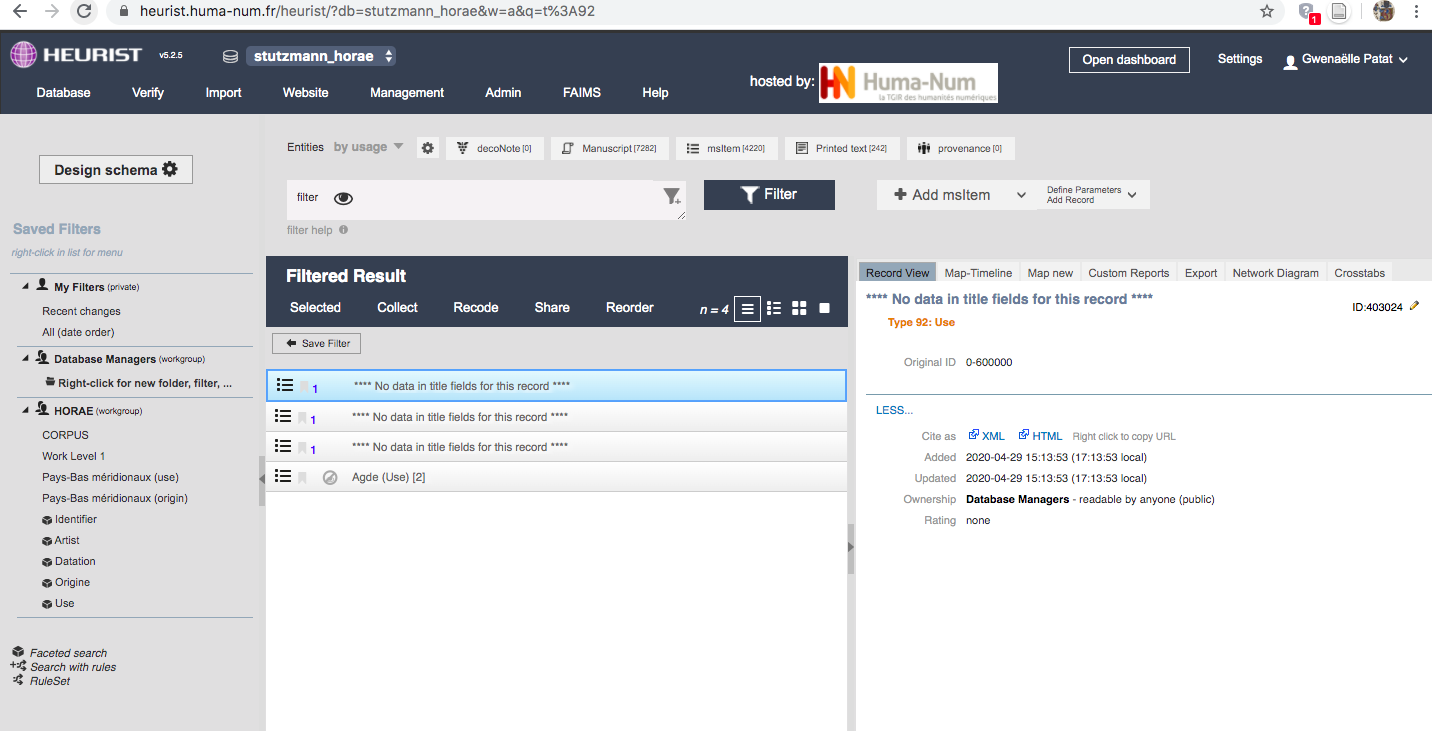
\includegraphics[width=15cm]{img/Import_Donnees/resultatTestXML1Use.png}
    \caption{Test d'import en XML de l'entité Use}
    \end{figure}
    
    \begin{figure}[!h]
    \centering
    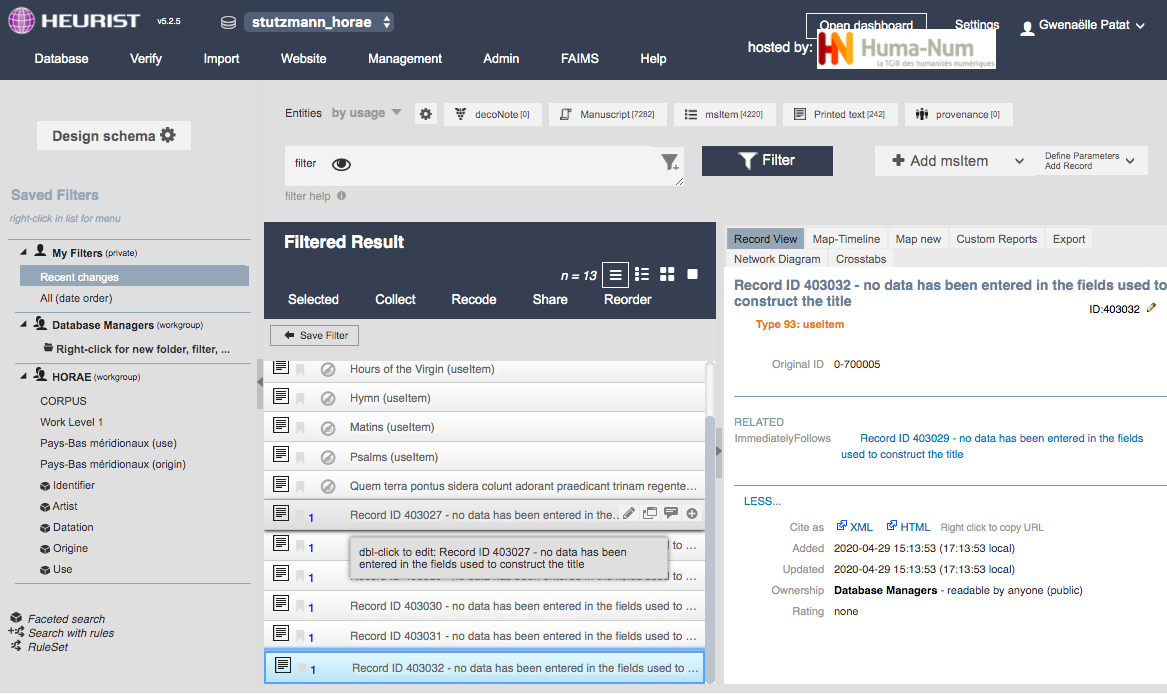
\includegraphics[width=15cm]{img/Import_Donnees/ImportTestXMLUseItem1.png}
    \caption{Test d'import en XML de l'entité UseItem}
    \end{figure}
    \clearpage
    
    \begin{figure}[!h]
    \centering
    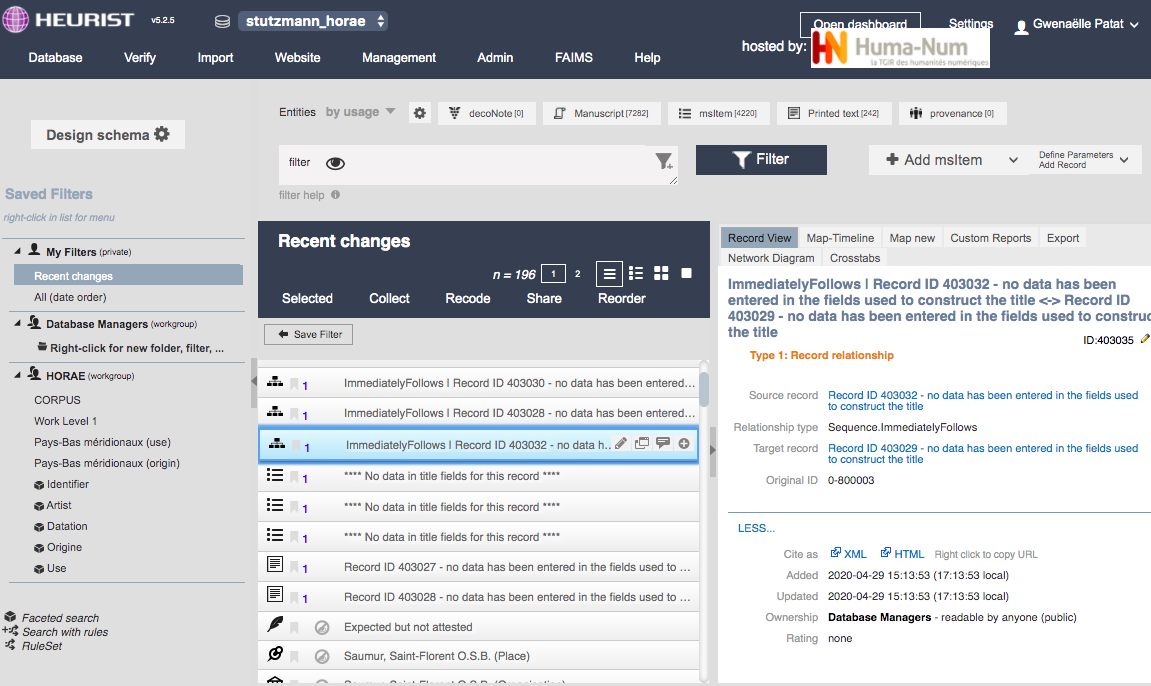
\includegraphics[width=15cm]{img/Import_Donnees/ImportTestXMLRelation.png}
    \caption{Test d'import en XML de l'entité Work}
    \end{figure}

La balise \textless title\textgreater~pour nommer les instances ne semble pas avoir de conséquence dans l'implémentation. \\

Nous avons en fait appris par la suite l'existence d'un template hml servant à l'import des données en xml : Template\_stutzmann\_horae\_20200429152715.hml. Si le document d'export en xml a permis de cerner le fonctionnement de la base Heurist, ce qui est à créer au moment de l'import et ce qui est généré par la base, il est nécessaire de respecter strictement le template indiqué pour réussir l'import. Le titre donné aux entités doit 
être défini dans la balise suivante :
\begin{minted}{xml}
<detail conceptID="2-1" name="Title">TEXT</detail>
\end{minted}
Le document cible a donc été re-pensé à partir du premier essai, dont voici un extrait\footnote{Vous trouverez le document cible dans son intégralité en annexes, section \ref{def_cible}.} : 
\begin{minted}{xml}
[...]
        <record>
            <id>H-ID-600000</id>
            <type conceptId="0000-92">Use</type>
            <detail conceptID="2-1" name="Title">Agen 
            (Use) [2]</detail>
            <detail conceptID="2-21" name="Organisation" 
            isRecordPointer="true">402892</detail>
        </record>
[...]
        <record>
            <id>H-ID-700000</id>
            <type conceptID="0000-93">useItem</type>
            <detail conceptID="0000-1134" name="Work" 
            isRecordPointer="true">H-ID-395039</detail>
            <detail conceptID="0000-1188" name="Work (Cursus)">
            Quem terra pontus sidera colunt
                adorant praedicant trinam regentem machinam 
                claustrum Mariae bajulat ; Cui luna sol
                et omnia deserviunt per tempora perfusa caeli 
                gratia gestant puellae viscera ; Beata
                mater munere cujus supernus artifex mundum pugillo
                continens ventris sub arca
                clausus est ; Beata caeli nuntio fecunda sancto spiritu
                desideratus gentibus cujus
                per alvum fusus est ; Jesu tibi sit gloria qui natus
                es de virgine cum patre et almo
                spiritu in sempiterna saecula ; Amen [Hymn] (useItem)</detail>
        </record>
[...]
        <record>
            <!-- Matins : Contains : Quem terra pontus... -->
            <id>H-ID-800001</id>
            <type conceptID="2-1">Record relationship</type>
            <detail conceptID="2-1" name="Title for relationship">
            Contains | Matins (useItem) &amp;lt;-&amp;gt; Quem 
            terra pontus sidera colunt
                adorant praedicant trinam regentem machinam 
                claustrum Mariae bajulat ; Cui luna sol
                et omnia deserviunt per tempora perfusa caeli 
                gratia gestant puellae viscera ; Beata
                mater munere cujus supernus artifex mundum
                pugillo continens ventris sub arca
                clausus est ; Beata caeli nuntio fecunda 
                sancto spiritu desideratus gentibus cujus
                per alvum fusus est ; Jesu tibi sit gloria 
                qui natus es de virgine cum patre et almo
                spiritu in sempiterna saecula ; Amen [Hymn]
                (useItem)</detail>
            <detail conceptID="2-7" name="Source record" 
            isRecordPointer="true">H-ID-700003</detail>
            <detail conceptID="2-6" name="Relationship type"
            termID="3262" termConceptID="2-3262"
                ParentTerm="Overlap">Contains</detail>
            <detail conceptID="2-5" name="Target record" 
            isRecordPointer="true">H-ID-700000</detail>
        </record>
[...]
\end{minted}

Une fois le document cible défini, il reste à savoir comment le créer à partir de données classées dans un csv et d'identifiants à générer automatiquement.


	\subsection{Structurer les données : du CSV à l’XML en passant par Python}
	
	Pour générer un document d'import au format XML, il est nécessaire d'installer la librairie python lxml\footnote{Cf \url{https://docs.python.org/3/library/xml.etree.elementtree.html}.}. Elle permet de créer les balises dont nous avons besoin pour l'import (\textless hml\textgreater, \textless database\textgreater, \textless records\textgreater, \textless record\textgreater, \textless id\textgreater, \textless type\textgreater~et \textless detail\textgreater ), ainsi que les attributs associés (\textit{conceptID}, \textit{name}, \textit{isRecordPointer}, \textit{termID}, \textit{termConceptID}, \textit{ParentTerm})\footnote{Les différentes versions du code, qui a évolué avec la compréhension des problèmes et de ce qui est attendu en format cible, sont disponibles en annexes section \ref{code_python}.}. Chaque élément \textless record\textgreater~doit correspondre à une ligne d'enregistrement dans le csv, de la manière suivante : 
	\begin{minted}{python}
with open ("/Users/gwenaellepatat/Desktop/Stage_TNAH/MémoireHORAE
/BaseHeurist/Données/UseItem_Test_LL.csv") as csvfile:
    donnees_Heurist = csv.reader(csvfile, delimiter=';'
    , quotechar='"')
    #id_record = 599999
    for id_record, row in enumerate(donnees_Heurist,
    600000) :
        #id_record += 1
        record = etree.SubElement(records, "record")
        #Sous-éléments de la balise record
        id_node = etree.SubElement(record, "id")
        id_node.text = "H-ID-" + str(id_record)
	\end{minted}
L'identifiant a été choisi à partir du chiffre 600 000 pour ne pas créer d'interférences avec le test d'import des données en csv. La balise concernant l'enregistrement et son identifiant est donc générée par le code python et dépend du nombre d'entrées dans le csv. 

Toutefois l'élément \textless type\textgreater~est à créer à la fois depuis le csv et le document d'export XML de la base Heurist, car l'attribut conceptID se réfère à des identifiants propres à la base Heurist : 
\begin{minted}{python}
type_node = etree.SubElement(record, "type")
        #Valeurs d'attributs de la balise 
        #type dépendant de la base Heurist
        type_node.set("conceptID", exportXML.
        hml.records.record[0].type["conceptID"])
        #Récupération du nom de l'entité dans 
        l'élément type depuis le CSV
        for line in csvfile :
            type_node.text = str(row[1])
\end{minted}

Le plus délicat est la création des éléments \textless detail\textgreater . Il est certes aisé de récupérer les données adéquates à partir des csv, comme le montre l'exemple ci-dessous : 
\begin{minted}{python}
for id_record, row in enumerate(donnees_Heurist, 600000) :

        detail1 = etree.SubElement(record, "detail")
        if type_node.text == "Use" :
            detail1.set("conceptID", "2-1")
            detail1.set("name", "Title")
            detail1.text = str(row[1]) + " (Use) [2]"

\end{minted}
Il est cependant plus contraignant de créer les relations via l'utilisation de clés étrangères, car il n'est pas possible de toutes les obtenir depuis le document d'export chargé. Cela dépend des données préalablement implémentées dans la base et de leur attribution d'un identifiant par Heurist pour pouvoir faire correctement les liens entre les entités, notamment les entités relevant de l'\og Organisation\fg{} pour les usages et de \og Work\fg{} pour les pièces liturgiques. Pour pallier ce problème, il faudrait d'abord générer des entités vides sans attributs et sans relations, pour ensuite récupérer l'identifiant d'Heurist à partir du document d'export XML et les appeler au bon endroit dans le code pour le nouveau document d'import, qui ferait cette fois-ci les jointures. Ces réflexions nous amènent à exposer plus en détail les raisons du choix d'importer les données en CSV. 

	
	\subsection{Raisons du choix d’importer les données depuis le format CSV}
	
Pour l'import des données en XML, le template défini pour la base Heurist indique un certain nombre de balises \textless detail\textgreater~ par entité. Elles peuvent être d'ordre textuel pour indiquer le contenu des données, ou bien elles servent à créer un lien vers une référence numérique pointant vers une autre entité. Toutes les balises \textless detail\textgreater~indiquées dans le template ne sont pas obligatoirement remplies au moment de l'import, car nous disposons souvent de données imparfaites. Il est toutefois possible de vérifier leur intégrité sur Heurist.
	
	Le template d'import en XML doit donc être pensé en amont de la modélisation des données, afin que tous les champs qui caractérisent la donnée apparaissent bien via une balise \textless detail\textgreater . En effet, une fois le template implémenté, il n'est plus possible de le modifier et il faut s'y conformer pour la bonne intégration des données dans la base. Ainsi, le template pour l'entité Use permet de faire un lien vers un UseItem :
	\begin{minted}{xml}
<detail conceptID="2-9" name="Date">DATE</detail>
<detail conceptID="2-21" name="Organisation" isRecordPointer="true">
RECORD_REFERENCE</detail>
<detail conceptID="0000-1011" name="bibl" isRecordPointer="true">
RECORD_REFERENCE</detail>
<detail conceptID="0000-1012" name="Note">MEMO_TEXT</detail>
<detail conceptID="0000-1181" name="UseItem" isRecordPointer="true">
RECORD_REFERENCE</detail>
<detail conceptID="0000-1187" name="Office">TEXT</detail>
	\end{minted}
	
Cependant, deux types de useItem apparaissent dans le modèle. L'entité useItem avec les champs suivants :
	\begin{minted}{xml}
<detail conceptID="0000-1012" name="Note">MEMO_TEXT</detail>
<detail conceptID="0000-1134" name="Work" isRecordPointer="true">
RECORD_REF</detail>
<detail conceptID="0000-1188" name="Work (Cursus)">TEXT</detail>
<detail conceptID="0000-1192" name="Sequence">TEXT</detail>
	\end{minted}
Puis on est confronté à l'entité useItem2 qui présente un champ différent, celui de la relation de succession des pièces :
\begin{minted}{xml}
<detail conceptID="0000-1012" name="Note">MEMO_TEXT</detail>
<detail conceptID="0000-1134" name="Work" isRecordPointer="true">
RECORD_REFERENCE</detail>
<detail conceptID="0000-1188" name="Work (Cursus)">TEXT</detail>
<detail conceptID="0000-1192" name="Follow">TEXT</detail>
\end{minted}
Toutefois, l'entité useItem2 n'est référencée ni par le premier useItem, ni par l'entité Use, ce qui pourrait poser des problèmes d'intégrité dans l'import des données si nous choisissons ce format.

	Par ailleurs, pour pouvoir faire les renvois vers les bons identifiants, il faut que les \textit{records-id} soient générés préalablement dans la base. La meilleure stratégie à adopter pour effectuer l'import des données en XML est donc d'agir en deux temps :
	\begin{itemize}
	    \item Faire un premier import pour générer les identifiants à partir des données brutes ;
	    \item Faire un deuxième import pour faire les liens entre les données avec la récupération des \textit{records-id} générés par Heurist.
	\end{itemize}
	
L'import en csv, usage par usage\footnote{Chaque usage a été séparé dans des csv différents, pour les raison expliquées ci-dessus.}, a donc été préféré pour garantir la cohérence des données. En effet, de tout importer dans un même csv pourrait engendrer une insertion des pièces liturgiques dans le désordre. Contrairement à d'autres projets, l'ordre des données n'est pas indifférent. Le projet HORAE présente ainsi une demande rare, celui d'un ordre dans les \textit{recordPointer}, car le modèle est structuré en hiérarchie comme dans un arbre XML. L’ordre des pièces doit refléter l’ordre de présence dans les manuscrits. En effet, chaque œuvre a un attribut de séquence pour ce qui précède et ce qui suit avec des renvois vers les œuvres concernées. L’ordre n'est donc ici pas déterminé selon l’identifiant ou la date mais selon la position de la pièce. 

De plus, il s’agit de faire les liens entre les usages et les pièces. On crée donc dans un premier temps les entités useItem dotées des bonnes associations avec les entités Work et les incipits, puis on importe dans un deuxième temps le cursus, soit les relations de succession et de hiérarchie entre les pièces liturgiques. Toutefois, la création de relations entre les useItem a tout de même désordonné la succession des textes au sein des Use. La solution ponctuelle a donc été de donner un attribut de séquence numérique au titre pour replacer les pièces dans le bon ordre de succession.\\

\textit{In fine}, le principal obstacle rencontré lors de l'import des données est une question de méréologie\footnote{Logique traitant les relations des parties à un ensemble.}, car chaque useItem a deux types de relation :
\begin{itemize}
    \item La section dans laquelle elle se trouve ;
    \item L'ordonnancement (ce qui précède ou ce qui suit).
\end{itemize}

Il est alors nécessaire de simplifier le modèle pour l’import, tout en lui faisant refléter la complexité de la réalité décrite. Il faut ainsi d’abord vérifier que l’import fonctionne avant de créer la structure. Cette opération fait se croiser trois thématiques importantes dans le traitement des données : 
\begin{itemize}
    \item La récupération des données héritées ;
    \item La sécurisation des données ;
    \item Les contraintes à définir pour garantir l'intégrité des données.
\end{itemize}
Ainsi la contrainte sur la structuration des données doit-elle permettre leur interopérabilité. D'un point de vue méthodologique, il est important d'identifier ce qui est générique et ce qui est spécifique. La priorité doit être accordée au générique, dans la mesure du possible. Il faut donc trouver les solutions les plus génériques possibles pour tenir compte des nouveautés, c'est-à-dire identifier ce qui est nouveau et le placer sous la bonne étiquette générique.

La vérification de l’intégrité des données peut se faire rapidement par un export de la base en xml, puis, grâce à une feuille xsl, on applique au document la fonction \textit{count()} pour voir les identifiants des œuvres qui pointeraient vers plus de 2 éléments, ce qui signifierait une erreur, car chaque identifiant doit être unique.\\

En ce qui concerne le travail de désambiguïsation de l'Office de la Vierge, il a consisté à compléter le travail de Victor Leroquais et Éric Drigsdahl. En effet, s'ils ont su relever les particularités liturgiques de chaque usage - nous en disposons d'environ 215 - nous n'avons accès qu'aux inicpits des différentes pièces, ce qui n'est pas suffisant pour les identifier. Il s'agit donc de reprendre les manuscrits étudiés pour compléter la base de textes disponibles. Cela a donné lieu à deux manières de signaler les particularités dans la base de données : 
\begin{itemize}
    \item \og \textit{Not identified}\fg{} pour les pièces restées mystérieuses\footnote{Dans la plupart des cas, il s'agit de bréviaires imprimés uniques, avec un seul exemplaire attribué, ce qui rend leur vérification impossible.} ;
    \item \og \textit{Expected but not attested}\fg{} pour les pièces absentes du manuscrit mais qui sont constitutives de l'usage dans lequel elles s'inscrivent\footnote{L'absence des pièces est mesurée à partir du travail sur les témoins d'Éric Drigsdahl. Cela concerne les pièces présentes dans l'usage mais pas dans le manuscrit, pour une raison quelconque. Cela est plus particulièrement le cas pour les antiennes de certaines heures, les hymnes ou les psaumes.}.
\end{itemize}\\

Toutefois, un problème subsiste. Si l’on découvre une pièce nouvelle, cela provoque un décalage dans la séquence, ce qui a des conséquences sur les autres pièces par ricochet. Chaque ajout d’une pièce implique la modification de deux autres. Le problème est le même pour les pièces à supprimer. Le projet HORAE montre dont le potentiel mais aussi les besoins d’adaptation du logiciel proposé, ce qui implique un dialogue constant avec les techniciens responsables du fonctionnement de la base de données.\\

L'import des données offre ainsi de nouvelles possibilités en visualisation des usages liturgiques, que ce soit du point de vue de leur géolocalisation que des pratiques de dévotion. 
	
	\section{Possibilités en visualisation des données}

	En sciences humaines et sociales, l'utilisation de bases de données relationnelles est le tremplin à la création de visualisations de systèmes complexes, d'archives textuelles ou d'œuvres multimédias. Cela peut se concrétiser par la publication d'une carte ou d'un site web. On peut penser au travail d'Éric Drigsdahl qui a mis en ligne différents usages localisés des Heures de la Vierge, d'Amiens à York en passant par Rennes\footcite{Usages_HVierge}. La définition de ces usages accessibles en ligne fournissent ainsi une référence dans l'étude des données du projet, mais elle offre aussi des possibilités d'enrichissement avec les nouvelles analyses résultant du projet. Ainsi, une base de données relationnelle bien conçue ne contient pas une liste d'informations statiques, mais tout un ensemble de relations ontologiques générant de nouvelles affirmations dans un domaine\footcite[Partie II, Chapitre 15]{Compagnon_DH}. 
	
	Le projet HORAE s'appuie sur un foisonnement de livres d'heures, d'une part décrits dans les notices, d'autre part numérisés selon le protocole IIIF et disponibles en lignes. L'approche quantitative sert ici une analyse qualitative afin de mieux visualiser le regroupement de manuscrits présentant les mêmes caractéristiques textuelles, avec l’ordre des différentes parties (petit office de la Vierge, offices votifs, suffrages, prières), mais aussi l’ordre des unités textuelles qui permet de repérer les usages liturgiques. Les visualisations possibles des données permettent donc de cerner la diffusion et la circulation des textes dévotionnels et liturgiques transmis par les livres d’heures du Moyen Âge pour mieux comprendre la culture et la foi des \textsc{XIII}\up{e}-\textsc{XVI}\up{e} siècles\footnote{Cf. présentation du projet sur le site de l'IRHT : \url{https://www.irht.cnrs.fr/?q=fr/recherche/les-programmes-de-recherche/horae}.}. Le projet montre donc que ce que l'on appelle \og humanités numériques\fg{} est avant tout une \og pratique de recherche\fg{}, selon les mots d'Aurélien Berra\footcite{Faire_HN}, une méthodologie.
	
	Une utilisation raisonnée du numérique pourrait ainsi répondre au souhait d'Ezio Ornato quant à la discipline de la codicologie, qu'il décrit comme une champ de réflexion prenant en considération tous les aspects du livre, de \og la nature des matériaux utilisés jusqu’aux modalités de conservation, de lecture et de diffusion, en passant par toutes les phases du processus de fabrication\fg{}\footcite[p. vii]{livre_medie}. Il parle donc de codicologie quantitative, nécessaire face à des données numériques, afin d‘accroître la performance des méthodes de datation, de localisation et d'attribution.\footcite[p. 41-47]{livre_medie}. Ces méthodes se fondent sur l'observation des techniques de fabrication du livre, croisant certaines variables comme la dimension des feuillets ou la disposition du texte\footnote{On trouvera une méthodologie d'observation des manuscrits médiévaux et de rédaction de notices appropriées plus précisément dans \cite{initiation_man_lit}}. Ainsi, les manuscrits à longues lignes sont globalement plus petits que ceux à deux colonnes\footcite[p. 51]{livre_medie}. Cette affirmation se vérifie dans les notices de Leroquais, où la majorité des manuscrits à longues lignes n'excèdent par les 299 mm de dimensions\footcite[Notice 145, p. 305]{Leroquais_notices}, tandis que ceux à deux colonnes peuvent dépasser les 300 mm de dimensions\footcite[Notice 5, p. 9]{Leroquais_notices}; Toutefois, cela n'exclut pas les manuscrits à deux colonnes de format plutôt petit\footcite[Notice 62, p. 150]{Leroquais_notices}. 
	
	\subsection{Géolocaliser les manuscrits et les usages}
	
	Dans une étude sur ce que recouvre le terme \og Humanités numériques\fg{} en France\footnote{Le terme est dérivé de la notion de \textit{digital humanities}, davantage formalisée dans le monde anglo-saxon.}, et plus particulièrement sur la question des mutations du support de l'écrit, Aurélien Berra rappelle que ce sont les usages qui font vivre les textes, et donc que les pratiques culturelles sont indissociables des techniques de production des manuscrits et imprimés, de leur profusion et de leur diffusion\footcite{Faire_HN}. 
	
En terme de géolocalisation de manuscrits du Moyen Âge et de la Renaissance, un projet réunissant l'IRHT, l'Université d'Oxford, de Pennsylvanie, et l'Université d'Aalto d'Helsinki, \textit{Mapping Manuscript Migrations}, rassemble depuis 2017 des données issues de sources variées afin d'analyser sur la plus large échelle possible l'histoire et la provenance des manuscrits\footnote{Cf. https://mappingmanuscriptmigrations.org/en/.}. Le projet est né de la nécessité de rassembler la prolifération de données numériques dispersées dans des catalogues et bases de données diverses\footcite[p. 249-250]{map_man_migration}. Un projet d'une telle ampleur soulève des questions méthodologiques sur la visualisation des données : comment représenter la complexité des métadonnées relatives aux manuscrits ? Le \textit{Linked data}, traduit par l'expression Web des données\footnote{Le terme est inventé et défini par Tim Berners-Lee, alors directeur du W3C. Il désigne la publication de données structurées sur le Web, non pas sous la forme de silos de données isolés les uns des autres, mais reliés entre eux pour constituer un réseau global d'informations qui rend les données plus visibles.}, permet alors de produire des cartes et des graphes de réseaux afin de favoriser de nouvelles façons de penser l'histoire et la provenance des manuscrits\footcite[p. 251]{map_man_migration}.

	
	De plus, la localisation des calendriers des livres d'heures reste un défi majeur. Établir des caractéristiques communes entre certains calendriers permet de définir des groupes issus d'aires géographiques et de périodes particulières\footcite[p. 781]{analyse_calendrier}. Si la majorité des calendriers contiennent des célébrations communes quant à la Vierge Marie, moins une fête est commune en-dehors d'un groupe, plus elle est caractéristique du groupe qui la célèbre\footcite[p. 781]{analyse_calendrier}. 
	
	Si le calendrier constitue donc un indice majeur pour la datation et la destination d'un manuscrit, il n'est pas le seul indicateur. Ainsi, dans les livres d'heures, les lignes vides sont rares dans un calendrier, ce qui aboutit parfois à la notation de fêtes de saints fautives. C'est plutôt la convergence de plusieurs signes distinctifs qui permet d'avancer des hypothèses sur un usage. Les litanies des saints sont ainsi un autre indice pour la localisation d'un manuscrit. Il reste toutefois difficile de localiser les livres d’heures car chaque section peut mêler des usages différents. Par exemple, l'office de la Vierge peut être à l’usage de Paris mais le calendrier à l’usage d’Arras.\\
	
	Cette complexité à inscrire le livre d'heures dans un usage précis s'explique par l'origine même de son apparition, et par sa place au sein des autres livres liturgiques. La liturgie votive devient de plus en plus prégnante à partir du \textsc{XIII}\up{e} siècle. Elle se structure sur un rythme hebdomadaire, mais son usage est local. Inspirée de cette pratique, la liturgie dévotionnelle se développe, sous une forme plus intime et moins communautaire, donnant une place particulière aux oraisons de saints. 
	
	Toutefois, les offices ne reflètent pas forcément les lieux de production et de destination, ce qui n’est pas le cas des autres livres liturgiques dont l’usage reflète la destination. Il faut alors distinguer l'usage de la destination, d'autant plus pour ce type de livre voué à la dévotion privée. Si l'on retrouve parfois des notes de possession ou des armoiries, le destinataire du manuscrit peut s'inspirer d’un usage qui n'est pas nécessairement lié à la localisation de son lieu de vie\footnote{Ces propos s'inspirent des séances de la formation continue délivrée par la spécialiste des manuscrits liturgiques Laura Albiero, \og Les livres liturgiques manuscrits et imprimés : principes de catalogage\fg{}.}. \\

Les possibles visualisations des données du projet HORAE s'inscrivent dans ce cadre. En ce qui concerne la géolocalisation, la base Heurist, grâce à des \textit{records pointers}, soit les clés étrangères, et des \textit{relationships makers}, les tables de relation, permet de choisir entre la cartographie des lieux de conservation des manuscrits et celle des usages. Il faut alors faire un \textit{ruleset}, une série de règles, pour afficher les lieux en question. Une version 6 est ainsi en cours de développement pour pouvoir visualiser les données sous forme de tables. Pour lors, il est possible de voir les lieux de conservation des manuscrits étudiés sur une carte : 
    \newpage
    \begin{figure}[!h]
    \centering
    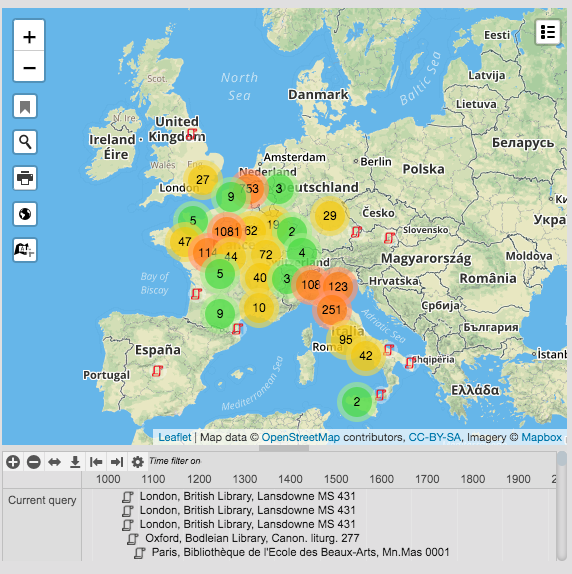
\includegraphics[width=15cm]{img/DataViz/Conservation_manuscrits.png}
    \caption{Cartographie des lieux de conservation des manuscrits étudiés}
    \end{figure}
    \clearpage

Ainsi que les lieux des différentes organisations évoquées :
    \begin{figure}[!h]
    \centering
    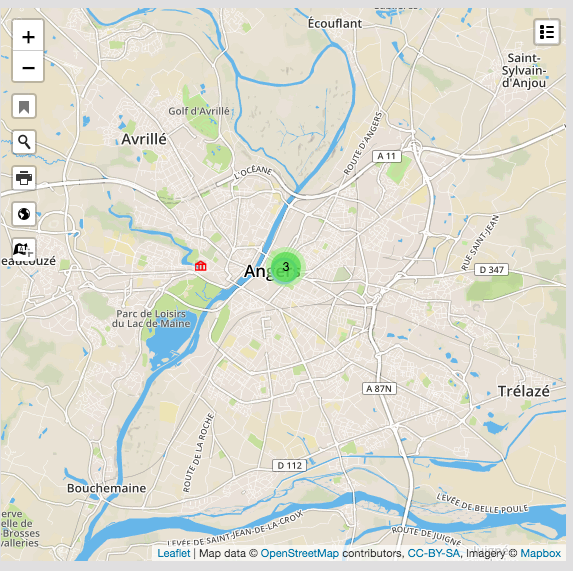
\includegraphics[width=10cm]{img/DataViz/Lieu_Organisation.png}
    \caption{Cartographie d'une organisation identifiée dans les usages des témoins : l'exemple d'Angers}
    \end{figure}
    \clearpage

	
	\subsection{Ce que nous disent les textes sur les dévotions…}
	

L'historienne Kathryn M. Rudy s'est intéressée à la manière dont les propriétaires de livres médiévaux, et plus particulièrement de livres d'heures du \textsc{XV}\up{e} siècle aux Pays-Bas, modifient le contenu de leurs livres pour refléter des situations changeantes, pas tant politiques que religieuses, économiques ou sociales\footcite[p. 1-2]{Piety_in_Pieces}. Les ajouts apportés à un livre peuvent ainsi témoigner d'une certaine force émotionnelle et sociale\footcite[p. 2]{Piety_in_Pieces}. Elle étudie donc les phénomènes de modifications d'un manuscrit, qui peuvent prendre la forme d'ajouts ou de soustractions\footnote{Parmi les phénomènes observés de contenu enlevé, on retrouve des traces de folios arrachés, de cahiers retirés, de textes grattés ou d'images dégradées.} de contenu, tout comme de changements dans l'organisation\footcite[p. 3]{Piety_in_Pieces}. Ces observations donnent des informations sur la manière dont les gens utilisaient et considéraient les livres de dévotion. L'historienne propose alors une nouvelle approche codicologique qui vise à comprendre quand un propriétaire de manuscrit complet et fini choisit de faire des ajouts pour signifier son appropriation : qu'est-ce qu'il gagne à le faire et qu'est-ce qui a rendu cela possible dans la structure des manuscrits\footcite[p. 5]{Piety_in_Pieces} ?

Kathryn M. Rudy divise les modifications apportées aux livres d'heures en deux catégories : celles qui impliquent une nouvelle reliure et celles qui n'en impliquent pas. Parmi la première catégorie, l'on retrouve des changements comme la correction du texte, l'ajout de texte entre les interstices ou sur les folios restés blancs\footnote{L'historienne est notamment confrontée à l'ajout d'informations familiales, de documents légaux, de gloses, d'informations sur les calendriers, de références à des circonstances particulières, d'explications pour faire du livre un outil didactique, ou de prières.}, l'agrandissement de décorations existantes, l'ajout de nouvelles illustrations, l'ajout de morceaux de parchemin sur les pages restées blanches, voire d'autres objets. Pour la deuxième catégorie, il s'agit de feuilles avec du texte ou des images. Ces images peuvent relever des offices les plus communs, ou bien d'indulgences, de portraits et de détails personnels, parfois provenant d'un autre manuscrit. Ce sont parfois des cahiers entiers qui sont ajoutés. Cela est rendu possible grâce à l'assemblage modulaire des manuscrits qui laissent plusieurs zones de parchemins blanches. En effet, le modèle pouvait être partagé entre plusieurs scribes auxquels était attribuée une portion de texte à copier\footcite[p. 89]{livre_medie}. Cette méthode de fabrication montre qu'un livre est pensé comme une construction progressive, un ensemble de fragments successivement ajoutés.\footcite[p. 9]{Piety_in_Pieces}. 
L'historienne analyse l'ajout de textes ou d'images à des manuscrits considérés comme complets comme des désirs relevant de différentes natures\footcite[p. 9]{Piety_in_Pieces} :
\begin{itemize}
    \item un désir de personnaliser le livre ;
    \item un désir de prendre possession des nouveaux sujets textuels ou visuels disponibles ;
    \item un désir de vouer sa dévotion à de nouvelles fêtes et cultes ;
    \item un désir d'ostentation de son pouvoir financier ;
    \item un désir de rehausser la décoration du manuscrit ;
    \item un désir de systématiser la décoration ;
    \item un désir de fixer des images volantes, parfois données en cadeaux. 
\end{itemize}
Ces désirs peuvent évidemment être mêlés. 

Il est également intéressant d'analyser les dévotions qui transparaissent dans les livres d'heures à partir du genre de leur commanditaire. Charity Scott-Stokes s'est par exemple intéressée aux livres d'heures produits en Angleterre et commandés par des femmes. Rappelant que le livre d'heures constitue un des livres les plus populaires auprès des laïcs de la fin du Moyen Âge, ils sont fondamentaux pour comprendre la piété médiévale, car son utilisation est principalement vouée au foyer. Ils sont donc révélateurs d'une dévotion ressentie dans l'intimité\footcite[p. 1]{Women_Books_Hours}. Elle observe entre autres une tendance un peu plus importante à célébrer les saintes féminines, en commençant par la Vierge et sainte Anne ; puis viennent les pénitentes du Nouveau Testament, comme Marie-Madeleine, et les vierges martyrs, notamment Catherine et Marguerite\footcite[p. 14]{Women_Books_Hours}. Ces saintes sont d'autant plus invoquées qu'elles sont associées au soulagement de douleurs et de maladies spécifiques. Ainsi, on fait appel à sainte Marguerite lors des accouchements, à sainte Apolline en cas de rage de dents, ou à sainte Suzanne pour protéger les femmes de la calomnie, des commérages et de la médisance\footcite[p. 15]{Women_Books_Hours}. \\

Dans le cadre du projet HORAE, il est encore trop tôt pour exposer d'éventuelles découvertes quant aux usages liturgiques et aux pratiques de dévotion. Il est toutefois possible de voir les relations entre les différentes pièces composant un livre d'heures sous forme de graphes : 
    \begin{figure}[!h]
    \centering
    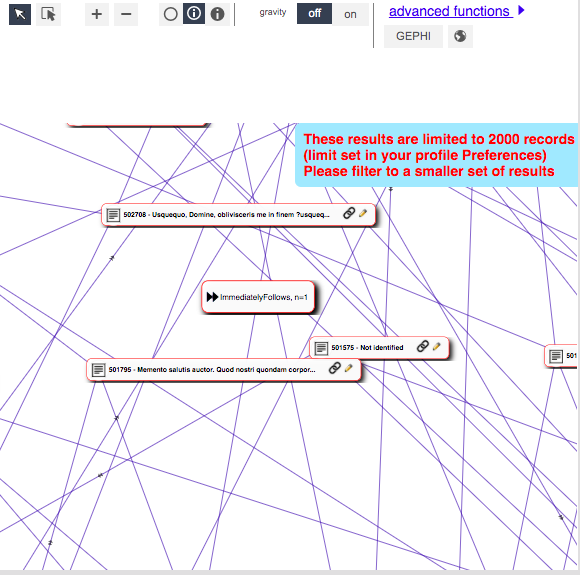
\includegraphics[width=10cm]{img/DataViz/réseau_section_livres_heures.png}
    \caption{Extrait de graphe sur les relations entre les différentes sections d'un livre d'heures}
    \end{figure}
    \clearpage

Ce qui ressort à présent des hypothèses formulées est la confirmation des analyses de Victor Leroquais quant aux variantes d'un même usage au sein de plusieurs témoins créés pour des commanditaires différents. Pour étudier plus amplement les dévotions, il est nécessaire de faire des liens entre les usages et les prières, ce qui est possible avec une plus grande prise de recul par rapport aux données amassées. En effet, l'idée est d'opérer un travail de comparaison des textes pour mieux déterminer les influences et les étendues des différents types de dévotion. \\

Bénéficier de données de qualité et pouvoir les visualiser est une première étape pour avancer des conclusions historiques, mais l’aventure ne s’arrête pas là. La reconnaissance automatique de textes et d’images et l'utilisation de l'intelligence artificielle permet de comparer des données en masse, et à terme, de définir les structures types de livres d’heures selon les usages liturgiques.

	
	\chapter{\label{ML}L’annotation pour l’apprentissage machine : ce que le numérique apporte à l’analyse des sources}
	
	L'utilisation de l'intelligence artificielle dans le cadre du projet HORAE, rendue possible grâce à la collaboration de différents acteurs dans les domaines de l'histoire et du numérique, montre la complémentarité des savoirs en humanités et en technologies. En effet,  il s'agit de rendre le savoir implicite en humanités explicite, afin de faire de ce savoir la clé de voûte de l'apprentissage machine, favorisant l'analyse de données en masse et leur formalisation. À partir d'un certain nombre de manuscrits annotés manuellement, processus selon lequel sont repérés les débuts de section de différents niveaux d'un panel de livres d'heures, une vérité terrain est établie. Le travail d'annotation, réalisé par les membres d'une institution spécialisée dans la recherche fondamentale sur les manuscrits médiévaux et les imprimés anciens, l'IRHT en l'occurrence, s'est opéré sur une interface développée par la \textit{start-up} Teklia. Les exigences relatives au projet ont ainsi permis au prestataire d'améliorer la qualité de ses services, tout en soulevant de nouveaux défis technologiques en terme de reconnaissance de texte, s'appuyant sur la vérité terrain définie préalablement. Les résultats technologiques obtenus interrogent alors sur les possibilités offertes par l'intelligence artificielle en terme d'analyse et de compréhensions de la structure des livres d'heures.
	
	
	\section{\label{gestion_management}Gestion et management d’un projet en humanités numériques}
	
	De la manière de gérer et manager un projet, et pas seulement en humanités numériques, découle sa réussite. Durant tout le projet, la coopération est continue, afin que tous les acteurs partagent la même vision managériale, soit les mêmes envies, et la même vision procédurale. Cette collaboration constante se concrétise par la planification de réunions régulières et l'affirmation claire et précise des échéances et des objectifs à atteindre, et ce dès le début du projet. Ces éléments se retrouvent dans des documents tels que la note de cadrage ou le cahier des charges. Les divers échanges et réunions entre l'IRHT, Teklia et le LS2N ont ainsi permis de clarifier les tâches et attentes de chacun, ce qui a notamment abouti à la mise en service d'une interface d'annotations conçue en partie dans le cadre du projet HORAE : Arkindex\footnote{L'interface de traitement automatique de document a vocation à se développer également au service d'autres projets. Cf. \cite{memoire_Chloe}}. 
	
	\subsection{La collaboration IRHT, Teklia et LS2N}
	
	Le cahier des charges du projet HORAE témoigne de l'importance d'impliquer chaque acteur du projet tout au long de ce dernier tout en définissant des tâches propres à chacun\footcite{HORAE_projet}.  Il rappelle dans un premier temps les objectifs du projet, son originalité et sa pertinence par rapport à l'état de l'art, ainsi que la méthodologie adoptée et la gestion des risques. Cette dernière partie se doit de témoigner de la conscience des potentielles déceptions du projet, et comment il est possible de les contourner, afin de rassurer les organismes financeurs. Pour HORAE, quatre grandes thématiques se détachent en terme d'apports et de risques : 
	\begin{enumerate}
	    \item \og Conséquences méthodologiques de la transdisciplinarité\fg{}. Il s'agit de mesurer l'efficacité d'un partenariat transdisciplinaire face à la gestion de données incertaines. En effet, les niveaux de qualité des données produites et analysées ne sont pas abordés de la même façon par les professionnels du numérique, qui cherchent à mesurer la précision d'une méthode d'analyse de document ou d'HTR\footnote{\textit{Handwitten Text Recongnition}.}, et par les chercheurs en humanités et l'éditeur de textes médiévaux qui ont besoin de données parfaites et qui ne peuvent quantifier l'incertitude. Le choix des partenaires d'HORAE est donc de s'appuyer sur des données \og bruitées\fg{} issues de l'HTR pour les associer à des unités textuelles de référence. Le cahier des charges prend l'exemple suivant : 
	    \begin{quote}
Par exemple, le verset \og \textit{In principio erat verbum et verbum erat apud Deum}\fg{} sera reconnu comme étant le premier verset de l’Évangile de Jean, même si on n’a que la séquence \og \textit{principio … verbum … Deum …}\fg{} en tenant compte de la faible distance séparant les mots. Ainsi, à partir de données fausses ou incomplètes, on peut arriver à une conclusion entièrement correcte.\footcite[p. 9]{HORAE_projet}
	    \end{quote}
	    De plus, pour vérifier les résultats des outils, des visualisations des données sont produites à chaque étape pour vérifier leur qualité et éventuellement les corriger, d'où l'importance de l'ergonomie pour la présentation des données. 
	    \item \og Analyse de document et reconnaissance d'écriture\fg{}. Il est ici question de mettre à profit le large corpus de manuscrits similaires par leurs structures et leur contenu pour développer les modèles de \textit{deep learning}. Leur développement est favorisé par la ré-utilisation de corpus mobilisés dans de précédents projets\footnote{Il s'agit des projets Oriflamms et Himanis. Le premier projet, acronyme de \textit{Ontology Research, Image Features, Letterform Analysis on Multilingual Medieval Scripts}, vise à analyser l'évolution des systèmes et formes graphiques des écritures au Moyen Âge selon leur contexte de production et leur langue. Une exposition des enjeux et des résultats du projet est disponible à l'adresses suivante : \url{https://oriflamms.hypotheses.org/1592}. Le deuxième projet, signifiant \textit{HIstorical MANuscript Indexing for user-controlled Search}, en partenariat avec les Archives nationales, a abouti à la création d'un moteur de recherche en plein texte dans les registres de la chancellerie royale. Une description plus ample du projet est disponible sur le site des Archives nationales, à l'adresse suivante : \url{http://www.archives-nationales.culture.gouv.fr/himanis}.}. L'autre enjeu est d'adapter les librairies \textit{open source}\footnote{Le terme \textit{open source} se réfère à l'accès à des codes sources que l'on peut librement réutilisés et redistribués. Ils sont souvent le fruit d'une collaboration entre programmeurs.} existantes aux manuscrits médiévaux. Le principal risque serait la production de résultats de qualité insuffisante pour identifier les textes, risque faible au vu des résultats acquis lors des précédents projets. 
	   \item \og Segmentation et identification des textes\fg{}. Les membres du projet y expliquent une méthode descendante de segmentation, qui consiste à à corriger la segmentation au fur et à  mesure de la reconnaissance de textes identifiés. 
	   \item \og Formats, visualisation, exploitation, pérennisation\fg{}. Cette partie rappelle l'utilisation de formats standards et de logiciels \textit{open source}. 
	\end{enumerate}\\
	
	Une deuxième grande partie revient sur l'organisation du projet les moyens mis en œuvre. Cette partie présente tout d'abord les principaux acteurs du projet, puis les cinq grandes tâches du projet, qui ne s'opèrent pas de manière successives mais croisées, selon les principes de la méthode dite \og Agile\fg{}. Elles recouvrent la constitution des données, les phases de recherche et développement, et la coordination.  À chaque tâche est rappelé un calendrier fixant des livrables et des échéances à atteindre, ainsi qu'une évaluation des risques. Les cinq étapes sont les suivantes : 
	\begin{enumerate}
	    \item \og Corpus, vérité terrain et modèle de données\fg{}. \\
	    
	    Principalement menées par l'IRHT, ces actions consistent à recenser les sources de livres d'heures disponibles en ligne et accessibles au format IIIF. Le projet prévoit d'impulser la numérisation de 99 de manuscrits microfilmés à la BnF et plus de 500 à l'IRHT, qui dispose déjà de trois bases de données recensant des livres d'heures\footnote{Parmi les bases de données constituées à l'IRHT et contenant des livres d'heures, on peut consulter la base Medium (\url{http://medium.irht.cnrs.fr/}), qui enregistre tous les manuscrits des bibliothèques françaises et étrangères dont l’IRHT détient des reproductions ; la base Iter Liturgicum Italicum (\url{https://liturgicum.irht.cnrs.fr/}), qui donne accès aux données relatives aux livres liturgiques d’origine italienne conservés en Italie et ailleurs, ou bien signalés dans les catalogues des maisons de vente ; la base INITIALE (\url{http://initiale.irht.cnrs.fr/}), qui recense les manuscrit enluminés conservés principalement dans les bibliothèques publiques de France hors la Bibliothèque nationale ; et enfin la base Bibale (\url{http://bibale.irht.cnrs.fr/}, créant des liens entre les notices pour rassembler les données de provenance de bibliothèques françaises.}. L'objectif est de créer un lot de plus de 120 000 images extraites de plus de 400 manuscrits. Les livrables concernent la mise à disposition des images numérisées.
	    
	    La deuxième sous-étape est la constitution du corpus textuel. Il s'agit de donner les moyens d'identifier les textes, ce que l'on appelle la \og vérité terrain\fg{}. Cette tâche bénéficie d'une double approche. D'une part, avec l'établissement d'unité textuelles de référence, formées d'un identifiant, d'un incipit et d'une version normalisée. D'autre part, grâce à la création de tables décrivant les principales structures des sous-sections, sections et parties d'un livre d'heures. Ce corpus est amené à s'accroître  avec la découverte de textes non prédictibles. Les  annexes de Victor Leroquais sont ainsi océrisées pour détecter les poèmes et prières inédits. Les livrables concernent donc la fixation de textes de références et de tables de structures. 
	    
	    La troisième sous-étape concerne des problématiques plus amplement abordées lors du stage : le modèle de données et l'unicité du format afin de garantir l'interopérabilité. Si l'affichage des manuscrits se fait selon le protocole IIIF, leur texte est encodé selon un modèle bien précis respectant la TEI, soit un schéma défini dans un document ODD comme nous l'avons présenté pour l'encodage des métadonnées, en l'occurrence des notices de livres d'heures conservées à la BnF. 
	    
	    La dernière sous-étape est la publication d'une interface graphique afin de saisir, visualiser et corriger les données si nécessaire, affiner la table de structure et les textes de référence\footcite[p. 11-13]{HORAE_projet}. On peut par exemple penser au mode auteur du logiciel Oxygen XML Editor qui permet de voir et modifier les données affichées de manière plus claire et limpide, sans balises, avec une présentation personnalisable grâce à la modification de la CSS et des frameworks du logiciel\footnote{Des tests de personnalisation de la CSS et des frameworks d'Oxygen sont disponibles dans les livrables techniques.}.\\ 
	    
	    \item \og Analyse et reconnaissance de documents\fg{}. \\
	    
	    Les tâches que recouvrent cette section concernent plus exclusivement la société Teklia. Une des premières étapes est d'opérer la classification des différents types de pages (couverture, page blanche, calendrier texte, texte illustré, etc.). L'objectif est de fournir une interface de visualisation des classes de page avec des fonctionnalités permettant de les regrouper selon leur type. 
	    
	    L'étape suivante est de détecter les lignes de texte. Si les livres d'heures présentent un cas plutôt simple au vu de leur homogénéité, soit des lignes horizontales de même hauteur alignées verticalement, certains éléments graphiques peuvent perturber la localisation des lignes, comme les lettrines et les illustrations. L'objectif principal est de fournir une interface de visualisation des zones de texte avec leur détection automatique. 
	    
	    L'étape logique qui en découle est la reconnaissance automatique de l'écriture manuscrite. Cette reconnaissance s'appuie sur des réseaux de neurones récurrents. Des librairies performantes sont disponibles en \textit{open source} comme la librairie \textit{TensorFlow} de Google\footnote{Outil d'apprentissage automatique fondé sur l'apprentissage profond, \textit{TensorFlow} est autant utilisé dans le milieu commercial que dans le monde de la recherche. Son code source est ouvert depuis 2015. Il est par exemple de plus en plus performant dans la reconnaissance de la parole.}. L'objectif est donc de présenter une interface de visualisation des textes avec une fonctionnalité de reconnaissance automatique des textes. 
	    
	    Enfin, la dernière étape consiste à développer une interface graphique pour traiter le corpus. Il s'agit de pouvoir appliquer la chaîne de traitement à tous les manuscrits et de présenter les résultats dans une interface web\footcite[p. 13-14]{HORAE_projet}. Cette étape se concrétise dans la mise à disposition de l'interface Arkindex utilisée pendant le stage. \\
	    
	    \item \og Segmentation et détection extrinsèque\fg{}. \\
	    
	    Cette partie est davantage menée par le Laboratoire des Sciences du Numérique de Nantes. La première étape consiste à segmenter les textes du livre d'heures. Cette segmentation se fait à trois niveaux, selon les sections, sous-sections et textes élémentaires. Il s'agit, à l'aide d'algorithmes, de mesurer une cohésion lexicale locale et globale adaptée aux livres d'heures, de calculer leur distribution au sein des sections et sous-sections, et de repérer les langues. Les livrables se concrétisent sous la forme de rapports sur la segmentation des livres d'heures et sur les algorithmes de segmentation.
	    
	    La deuxième étape s'apparente à l'identification des unités textuelles de référence. Cette identification est possible grâce à des expérimentations sur des empreintes, qui correspondent à des suites de n-grammes\footnote{Un n-gramme est une sous-séquence d'éléments construite à partir d'une séquence donnée. Il s'agit en fait d'établir des probabilités d'apparition d'une lettre ou d'un mot selon les textes élémentaires donnés.}. Les empreintes sont ensuite comparées selon des tests de mesures de similarité. Les livrables prennent la forme de rapports et de spécifications sur la détection extrinsèque des textes élémentaires. 
	    
	    Il s'agit ensuite de consolider la \og table des matières\fg{} des manuscrits étudiés, en mettant à jour les textes non-repérés auparavant. 
	    
	    Puis, vient le processus d'alignement des livres d'heures à partir d'un livre d'heures de référence. D'une part, le macro-alignement consiste à mettre en correspondance la structuration des textes avec les textes élémentaires de référence, afin d'identifier les textes non-référencés, les parties communes et les différences. D'autre part, le micro-alignement s'attache à mettre en regard les textes élémentaires entre livres d'heures afin de mieux visualiser les différences, les éventuelles fautes du programme de reconnaissance du document, mais aussi les possibles variations linguistiques. Les livrables correspondent à la visualisation des alignements. 
	    
	    Enfin, comme pour les grandes étapes précédentes, cette tâche se conclut par la création d'une interface de visualisation qui permet de valider les alignements de textes élémentaires détectés\footcite[p. 14-15]{HORAE_projet}. \\
	    
	    \item \og Création de savoirs à l'ère numérique : visualisations et interprétations\fg{}. \\
	    
	    Cette séquence de tâches concerne l'IRHT. Il s'agit de favoriser l'émergence de nouveaux savoirs grâce à l'intégration des résultats en vue d'une expérience utilisateur de qualité. Pour y parvenir, il faut coordonner et intégrer les différents développements en visualisation des données. Cette étape est exigeante en terme de fonctionnalités pour l'utilisateur final, notamment dans l'objectif d'enrichir les métadonnées et d'interagir avec les données. Un travail de veille sur les outils disponibles est donc indispensable. 
	    
	    La deuxième étape consiste à publier les données de la manière la plus pérenne possible. 
	    
	    La publication des données permet ensuite de mesurer les similarités et de visualiser les réseaux textuels. Il s'agit de repérer les textes inédits à partir des textes non alignés, de comparer les différentes structures des livres d'heures, d'identifier des usages liturgiques et de repérer des réseaux textuels via la visualisation de textes transmis ensemble et dans le même ordre. Cette étape nous rappelle l'importance de produire des données de qualité et de détenir des informations valides pour préserver la véracité des conclusions historiques. 
	    
	    La production de ces savoirs permet de diffuser une histoire des lectures dévotes du \textsc{XIII}\up{e} au \textsc{XVI}\up{e} siècles via l'écriture de deux monographies, ainsi que de la publication d'une anthologie de textes édités durant le projet\footcite[p. 15-16]{HORAE_projet}. \\
	    
	    \item \og Administration et communication\fg{}. Cette section rappelle les outils de communication pour le suivi du projet par les différents acteurs et la stratégie de diffusion\footcite[p. 16-17]{HORAE_projet}. Les métadonnées générées par le projet sont ainsi publiées sous licence libre sur Github\footnote{Cf. \url{https://github.com/oriflamms/HORAE}.}.\\
	    	\end{enumerate}
	    
	    La dernière grande partie du cahier des charges concerne les retombées du projet. Le caractère innovant du projet est en effet de proposer l'automatisation de la transcription et de l'identification de textes transmis par les manuscrits médiévaux. Par ailleurs, il participe à un changement majeur dans la transmission et la valorisation du patrimoine culturel. Ainsi, les conséquences dans le milieu scientifique sont triples\footcite[p. 17-18]{HORAE_projet} : 
	    \begin{itemize}
	        \item L'adaptation de librairies logicielles libres et \textit{open access} à l'analyse d'images et de textes de manuscrits médiévaux ;
	        \item L'analyse de dérivations textuelles en linguistique computationnelle ;
	        \item Le changement de l'approche en catalogage des manuscrits médiévaux et l'augmentation des connaissances du patrimoine textuel, de la liturgie, des échanges culturels de la fin du Moyen Âge en humanités. 
	    \end{itemize}\\
	    
	    Du point de vue culturel, HORAE s'inscrit dans la volonté des pouvoirs publics de rendre plus immédiatement accessible le patrimoine via la numérisation. Toutefois, la présence en ligne ne suffit pas pour être visible, et les objets culturels numérisés sont parfois peu exploités et expliqués. L'expertise scientifique et technologique développée lors du projet peut alors offrir de nouveaux moyens pour structurer les collections et les mettre à disposition du public de manière éclairée, compréhensible et interactive\footcite[p. 18]{HORAE_projet}.  
	    
	    Le projet HORAE reflète la \og révolution numérique\fg{} qui traverse nos sociétés. Le numérique est ici l'outil au centre de la création et du partage des savoirs, tout en favorisant auprès du grand public la découverte par sérendipité\footcite[p. 18-19]{HORAE_projet}. \\
	    
	    Lors du stage, le management du projet s'est cristallisé lors des diverses réunions entre les principaux acteurs. Ces réunions régulières sont essentielles pour s'informer et informer à propos des livrables acquis et de ceux qu'il reste à fournir. Dans le projet HORAE, le client, l'IRHT, institution spécialisée dans les manuscrits anciens, s'engage à fournir des données historiques de qualité à exploiter, tandis que la \textit{start-up} Teklia, son prestataire, garantit la mise à disposition d'outils numériques nécessaires pour l'analyse des sources, selon les objectifs définis dans le cahier des charges. Lors du stage, la collaboration entre le client et son prestataire s'est essentiellement focalisée sur le perfectionnement de l'interface Arkindex, afin qu'elle soit la plus efficace et la plus ergonomique possible. 

	
	\subsection{\label{arkindex}Arkindex : une interface d’annotation en construction}
	
		Arkindex est une plateforme de traitement automatique des documents, de la classification des pages à la reconnaissance d’écritures manuscrites en passant par la détection des lignes. Nos premiers pas sur Arkindex se sont effectués autour du travail d'annotation, c'est-à-dire le repérage des débuts de section d'un corpus de livre d'heures, selon un protocole sur lequel nous reviendrons. L'équipe de l'IRHT s'est tout d'abord heurtée à des problèmes liés à l'ergonomie de l'interface, notamment à propos de l'impossibilité de zoomer sur les pages numérisées et du déplacement du rectangle de sélection selon la résolution de l'écran. 
		
	Pour régler le problème de la sélection de la zone d’annotation qui dépend de la résolution de l’écran, des tests ont été effectués avec des résolutions différentes afin de stocker les données en fonction. Le résultat final doit être que l'alignement de la ligne du texte corresponde à la sélection, sans que la résolution soit en jeu.
	
	 Par ailleurs, les problèmes de performance dus au trop grand nombre de requêtes sur la base de données ont été résolus grâce à l'installation d’un système en clusters. Cela signifie le partitionnement des données sur plusieurs serveurs afin de gagner en rapidité dans le temps de réponse. \\
	 
	\begin{figure}[!h]
    \centering
    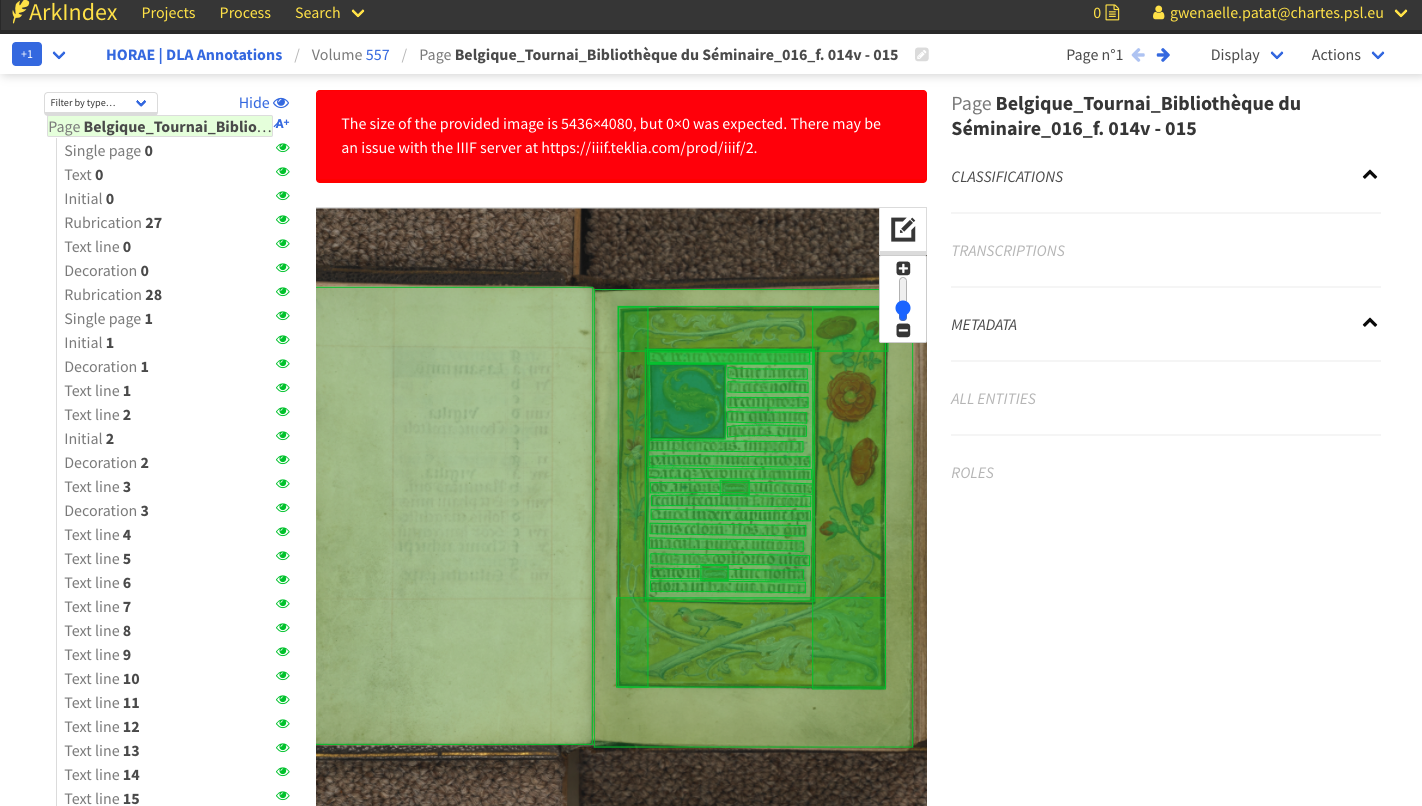
\includegraphics[width=13cm]{img/ML/interface_arkindex_detection_page.png}

    \caption{Exemple des différentes classes de segmentation d'une page de livre d'heures sur l'interface Arkindex}
    \end{figure}
	
	Un corpus spécifique pour l'inter-annotation\footnote{Il s'agit d'un ensemble de 10 manuscrits communs à plusieurs annotateurs de l'IRHT pour établir la vérité terrain sur les sections à l'intérieur des livres d'heures.} a été préparé avec l’ensemble des classes à gérer\footnote{Les classes correspondent à tous les contenus d'annotation, qu’il s’agisse des textes ou des niveaux hiérarchiques. Le contenu des classes sera plus explicitement abordé lors de l'explication du protocole d'annotation dans la section \ref{protocole_annotation}.}. On en compte environ 4500. L’objectif est de pouvoir faire des recherches avancées dans les classes et la base de données, ce qui implique un travail de développement important du côté de Teklia pour accroître la performance d'Arkindex. En effet, à la différence du logiciel Mirador\footnote{Cf. \url{https://projectmirador.org/}. Mirador est un visualiseur web qui offre des fonctionnalités avancées de zoom, de comparaison et d'annotation d’images en haute résolution, indépendamment du type de document ou de la bibliothèque numérique qui les héberge. Il permet d'afficher dans une interface commune des documents numériques provenant d'entrepôts d'images différents et compatibles avec les protocoles IIIF.}, on doit pouvoir faire une recherche dans une liste. 
	
Il convient de revenir sur le terme de \og classe\fg{}. La classe est un terme générique propre aux tâches du \textit{data mining}\footnote{Le \textit{data mining} désigne le procédé pour trouver des corrélations entre de nombreuses bases de données relationnelles. Ces corrélations peuvent prendre la forme d'associations, des modèles au sein desquels un événement est lié à un autre événement ; d'analyse de séquence, soit des situations au sein desquelles un événement mène à un autre événement plus tardif ; de classification et de \textit{clustering} comme dans le cadre du projet HORAE ; ou de prédiction.}, avec d’une part, la classification, et d’autre part, le \textit{clustering}. La classification consiste à déterminer le nombre de catégories à traiter \textit{a priori}. Chaque élément est donc associé à une classe. Quant au \textit{clustering}, le partitionnement de données, il fait référence à un ensemble d’éléments dont on doit optimiser le regroupement. Il s'agit en fait d'analyser les données en les regroupant dans différents paquets homogènes, c'est-à-dire partageant des caractéristiques communes. Les données sont alors regroupées dans des ensembles et des sous-ensembles reliés entre eux.\\

Pour la détection de ligne, le modèle est entraîné à partir du corpus de livres d'heures, selon les principes du \textit{deep learning}. Grâce à l'insertion en image d’entrée des caractéristiques d’une ligne, la machine génère une image de prédiction au niveau pixel. Le \textit{deep learning} est en effet un type d'intelligence artificielle dérivé du \textit{machine learning}, où la machine est capable d'apprendre par elle-même, sans règles pré-déterminées par un programme. 
	\begin{figure}[!h]
    \centering
    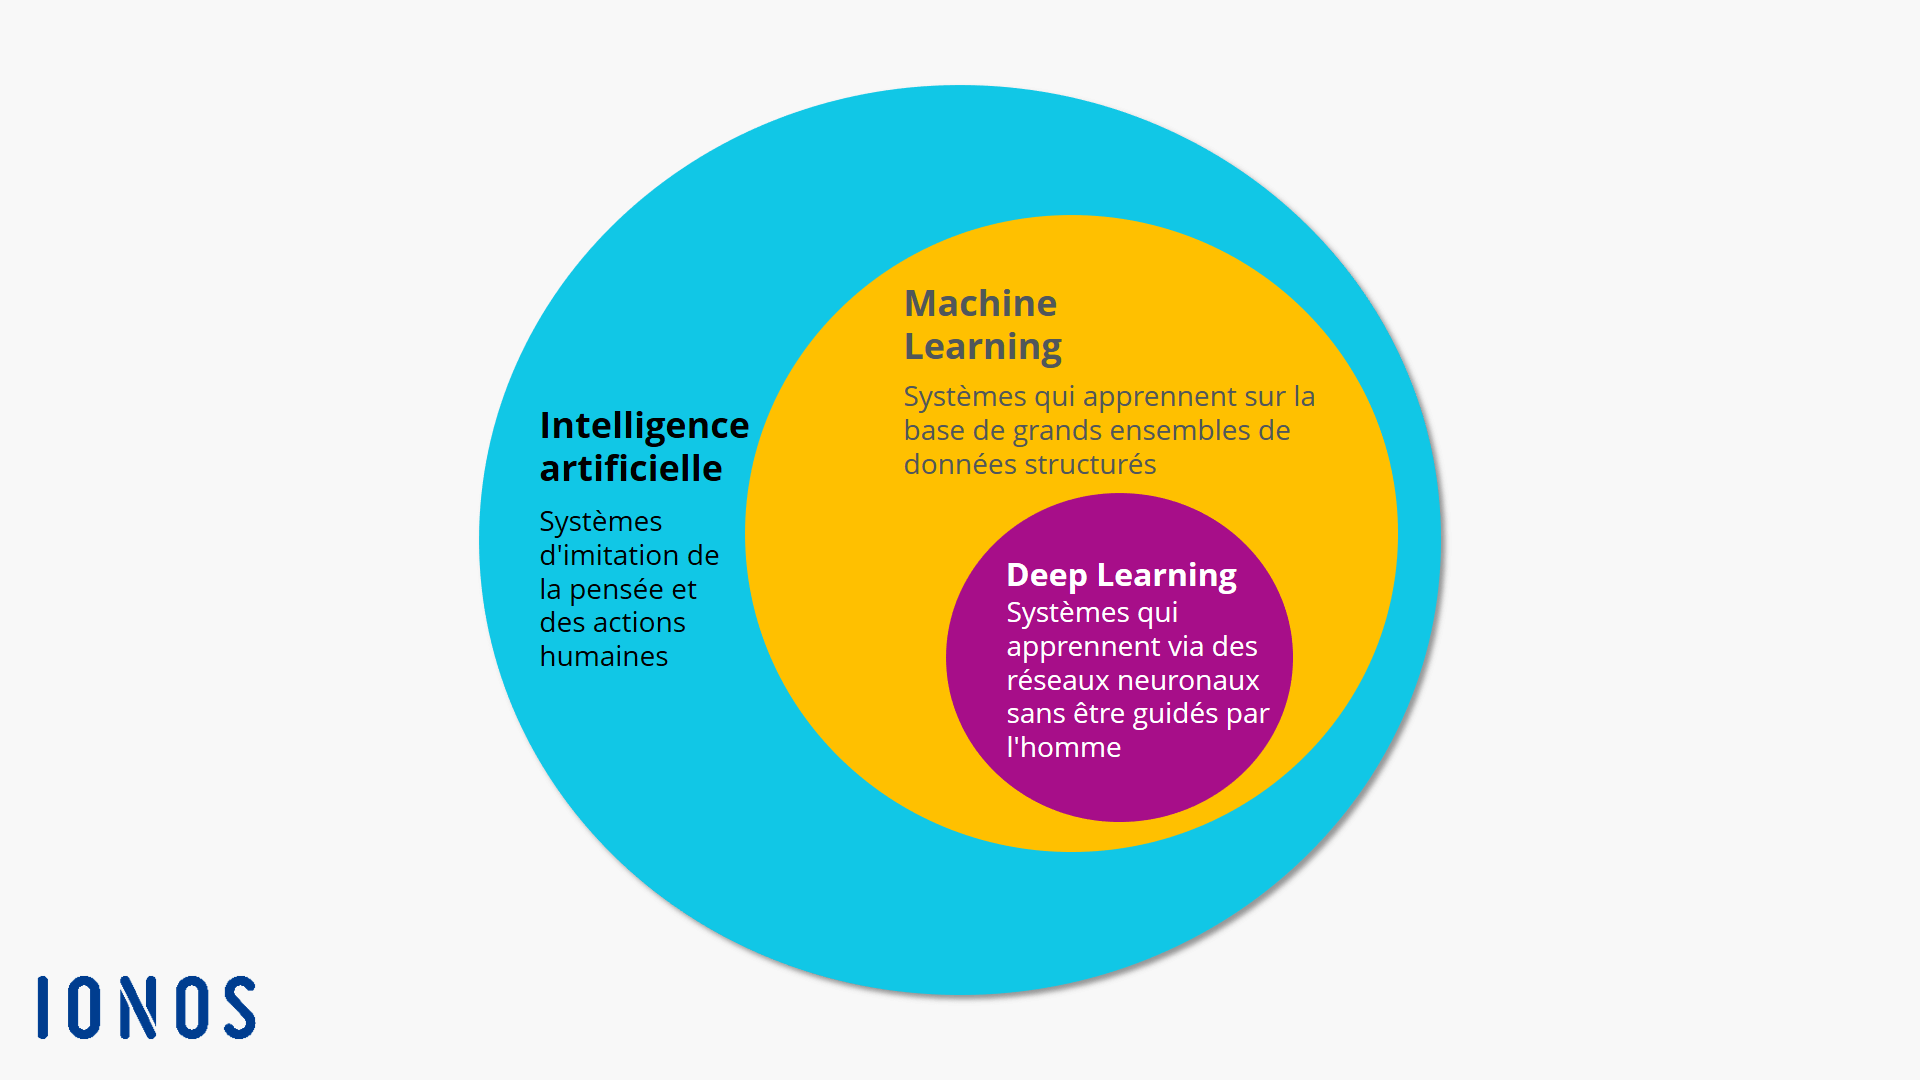
\includegraphics[width=13cm]{img/ML/schema_deep_learning.png}
    \caption{L'imbrication du \textit{deep learning}, du \textit{machine learning} et de l'intelligence artificielle. Cf. \cite{Difference_deeplearning_machinelearning}}
    \end{figure}
Il s'appuie sur un réseau de neurones artificiels qui s'entraînent à identifier des objets, lettres ou visages, selon les données de départ, qui sont donc essentielles à l'entraînement du modèle. Plus les données de départ sont variées, plus le système sera performant. Dans le cas d'HORAE, la reconnaissance des lignes est une étape primordiale, car elle influe sur la qualité de la reconnaissance de texte. Il faut alors tester le modèle selon les types de lignes, qui peuvent 
être plus ou moins droites sur l'image selon la qualité de la numérisation. En effet, les qualités de numérisation sont disparates, concernant parfois le document lui-même, parfois simplement le microfilm. \\

 Le développement de l'interface inter-annotateur Akindex montre l'importance de faire une interface test dans un premier temps pour ensuite comprendre les points à améliorer. En effet, meilleure est l'ergonomie, meilleure est la qualité des données. La mise en place de l'interface Arkindex a permis d'appliquer le protocole d'annotation afin d’établir une vérité terrain pour entraîner la reconnaissance automatique de textes et de sections au sein des livres d'heures. 


	\section{\label{protocole_annotation}Le protocole d’annotation pour guider l’apprentissage machine}
	
	Pour entraîner le modèle qui doit restituer des données de qualité, une vérité terrain a été établie par les membres de l'IRHT. Elle a été établie grâce à un protocole expliqué dans un manuel d'annotation qui rappelle les niveaux hiérarchiques et les pièces que l'on peut retrouver dans un livre d'heures. Quatre niveaux hiérarchiques ont donc été établis selon les parties structurelles des livres d'heures. Le premier niveau est composé des principales parties du livre d'heures, et contient 74 classes principales. Voici les plus fréquentes :
	\begin{itemize}
	    \item \textit{Calendar}
        \item \textit{Gospel Lections}
        \item \textit{Hours of the Cross}
        \item \textit{Hours of the Holy Spirit}
        \item \textit{Hours of the Virgin}
        \item \textit{Hours of the Virgin (Advent)}
        \item \textit{Hours of the Virgin (Temporale)}
        \item \textit{Litany of Mary}
        \item \textit{Mass}
        \item \textit{O intemerata}
        \item \textit{Obsecro Te}
        \item \textit{Office of the Dead}
        \item \textit{Office of the Dead (Temporale)}
        \item \textit{Penitential Psalms and Litany}
        \item \textit{Prayers}
        \item \textit{Psalter}
        \item \textit{Suffrages}
	\end{itemize} 
	\\
	
	
	Les classes de niveau 2 représentent logiquement une subdivision des contenus des sections de niveau 1. Si les classes de niveau 2 désignant des prières correspondent aux prières les plus couramment présentées dans les livres d’heures\footnote{Il s'agit des prières suivantes : Les \textit{Quinze Joies de la Vierge}, Les cinq psaumes pour Marie (\og \textit{Magnificat anima mea Dominum }\fg{} ; \of \textit{Ad Dominum, cum tribularer, clamavi}\fg{} ; \og \textit{Retribue servo tuo, vivitica me et custodiam sermones tuos }\fg{} ; \og \textit{In convertendo Dominus captivitatem Sion }\fg{} ; \og \textit{Ad te levavi oculos meos qui habitas in coelis }\fg{}), les \textit{Sept requêtes à notre Seigneur}, les \textit{Sept vers de saint Bernard}.}, les autres prières sont à annoter au niveau 1, avec la classe \og Prayers\fg{}. Ce tableau résume l'imbrication des niveaux 1 et 2 : 

\begin{table}[h!]
\centering
\begin{longtable}{|c|c|}
\hline
\textbf{Niveau 1} & \textbf{Niveau 2} \\ 
\hline
Calendar & January \\ 
& February \\ 
& March \\ 
& April \\ 
& May \\ 
& June \\ 
& July \\ 
& August \\ 
& September \\ 
& October \\ 
& November \\ 
& December \\ 
\hline
Gospel Lections & Gospel of John \\
& Gospel of Luke \\
& Gospel of Matthew \\
& Gospel of Mark \\
& Passion (St John) \\ 
\hline
Hours of the Cross & Matins\\ 
Hours of the Holy Spirit & Lauds\\
Hours of the Virgin & Prime\\
Hours of the Virgin (Advent) & Terce\\
Hours of the Virgin (Temporale) &  Sext\\ 
& None \\
& Vespers \\
& Compline \\
& Multiple hours \\ 
\hline
Mass & Preparation \\
& Readings \\
& Oblation \\
& Consecration \\
& Communion \\
& Conclusion \\ 
\hline
Office of the Dead & Vespers\\
Office of the Dead (Temporale) &  Matins\\
& Lauds  \\
\hline
Prayers & Fifteen Joys of the Virgin \\
& Five Psalms for Mary \\
& Seven Things which Please God \\
& Verses of St Bernard \\ 
\cline{1-2}
\end{longtable}
\end{table}
\clearpage
\begin{table}[h!]
\centering
\begin{longtable}{|c|c|}
\hline
Penitential Psalms and Litany & Penitential Psalms \\
& Litany \\ 
\hline
Credo &\\
Litany of Mary &\\
O intemerata &\\
Obsecro Te &\\
Office in the chapter &\\
Paschal table & \\ 
\hline
Suffrages & Angeli \\
& Anna \\
& Antonius \\
& Apollonia \\
& Barbara \\
& Blasius \\
& Catharina \\
& Christophorus \\
& Elisabeth \\
& Eutropius \\
& Georgius \\
& Geraldus \\
& Gregorius \\
& Jacobus \\
& Johannes Baptista \\
& Johannes evangelista \\
& Laurentius \\
& Margareta \\
& Maria Magdalena \\
& Martinus \\
& Martyres \\
& Michael \\
& Multiple hours \\
& Nicolaus \\
& Omnes apostoli \\
& Omnes sancti \\
& Paulus \\
& Petrus \\
& Petrus et Paulus \\
& Roch \\
& Sebastianus \\
& Stephanus \\
& Trinitas \\
& Veronica \\ 
\cline{1-2}
\end{longtable}
\caption{Imbrication des niveaux 1 et 2 selon la structure des livres d'heures}
\end{table} 

Il convient de faire la distinction entre les Heures de la Vierge, les Heures de la Vierge pour le temps de l'Avent\footnote{Le temps de l'Avent désigne la période qui s'étend du quatrième dimanche précédent Noël à la veille de la fête. Il correspond au début de l'année liturgique.} et les Heures de la Vierge dans le Temporal\footnote{Le temporal désigne l'organisation de l'année liturgique, du premier dimanche de l'Avent au premier dimanche après la Pentecôte. Il s'oppose au sanctoral, qui désigne la célébration des saints.}. Elles dépendent de la partie de l’année liturgique. On peut s’appuyer sur le texte et les rubriques pour les distinguer, mais les plus courantes sont les Heures de la Vierge.\\

Le troisième niveau, ignoré des copistes, signale l'ordonnancement du cursus dans chaque office, et constitue donc une sous-partie des niveaux 2. On y retrouve les pièces liturgiques suivantes : 
\begin{itemize}
    \item \textit{Canticle}\footnote{Chant extrait de l'Ancien ou du Nouveau Testament selon où on se trouve dans le cursus.} ;
    \item \textit{HSL}\footnote{Abréviation pour \og \textit{Hymn - Short lesson}\fg{}, ces deux sections constituent une unité au sein des laudes, des vêpres et des complies.} ;
    \item \textit{Hymn}\footnote{Chant poétique pouvant être rythmé, métrique ou rythmique.} ;
    \item \textit{Invitatory}\footnote{L'invitatoire peut désigner l'antienne en introduction des matines ainsi que le psaume qu'il l'accompagne, mais aussi l'antienne en elle-même se concluant par les mots \og \textit{Venite adoremus}\fg{}.} ;
    \item \textit{Invocation}\footnote{Il s'agit d'une formule introductive de l'office, composée d'un versicule et sa réponse, empruntés aux psaumes 50 et 69 lors des matines et 69 pour les autres heures. Seul l'office des morts n'en possèdent pas.} ;
    \item \textit{Lessons}\footnote{Lecture d'origine scripturaire ou patristique.} ;
    \item \textit{Orationes}\footnote{Conclusion de l'office comprenant une suite d'oraisons et la salutation.} ;
    \item \textit{Preces}\footnote{Les \textit{preces} désignent la partie de l'office et de la litanie contenant des formules de supplication.} ;
    \item \textit{Psalms}\footnote{Pièce poétique extraite du livre biblique des psaumes. On en trouve 150 dans la tradition latine.} ;
    \item \textit{Short lesson}\footnote{Appelée capitule en français, il s'agit d'une courte lecture extraite de la Bible.}.
\end{itemize}
Toutefois, les heures abrégées de la Croix et du Saint-Esprit ne sont pas annotées avec le niveau 3. Il faut donc annoter le versicule d’invocation dans la section de niveau 2 correspondante, sachant que ces heures ne contiennent pas de laudes. Les annotations de niveau 3 ne concernent en fait que les Heures de la Vierge et l’Office des morts, les deux sections caractéristiques des livres d'heures.\\

Quant aux pièces de niveau 4, le plus fin niveau de granularité défini dans le cadre du projet, elles désignent principalement les textes élémentaires, dont l'accès est encore à implémenter dans Arkindex. En effet, les pièces de ce niveau sont les plus fécondes en surprises et en découvertes, et sont donc amenées à être ajournées. Elles recouvrent les différents chants, oraisons, prières ou lectures. Par exemple, l'annotation avec la catégorie \og \textit{test-class}\fg{} a permis de mettre en avant les saints qui n'étaient pas encore répertoriés dans les suffrages et de les ajouter au sein des classes\footnote{Si les prières à la Vierge \textit{Obsecro te} et \textit{O Intemerata} auraient dû logiquement faire partie du niveau 4, elles ont été placées en niveau 1 du fait de leur présence quasi systématique dans les livres d'heures.}.\\

L'annotation de ces différentes sections, et plus particulièrement de leur incipit, s'explique par leur caractère révélateur de l'usage liturgique employé. En effet, l'identification de l'usage ne nécessite pas un relevé complet des textes, mais les indices issus du petit office de la Vierge doivent être corroborés par ceux issus de l'office des morts et de la présence de saints locaux dans le calendrier et les litanies. Il suffit alors de relever les incipits des pièces de niveaux 2 et 3 dans le petite office de la Vierge et l'office des morts, puis de les comparer avec ceux établis par le chanoine Leroquais dans Paris, Bibl. nat. de France, n. acq. lat. 3162 (pochette microfilm IRHT n° 43251)\footcite[p. 105-106]{initiation_man_lit}.\\ 

L'objectif étant d'entraîner le modèle pour la reconnaissance automatique de texte, et \textit{in fine} des sections associées, des stratégies d'évolution ont été confirmées lors de la réunion du 17 juin dernier entre les trois partenaires du projet. Le travail consiste alors à ajouter des transcriptions, mêmes imparfaites\footnote{La méthodologie, dont on a rappelé les principes dans la section \ref{gestion_management}, consiste à utiliser des données imparfaites, c'est-à-dire qu'un texte de référence est plaqué sur le texte correspondant, même s'il contient d'éventuelles variantes textuelles, afin de parvenir à des conclusions historiques correctes, soit la bonne identification des sections des livres d'heures malgré les variantes textuelles. Les textes de référence établis pour les psaumes pénitentiels sont présentés en annexes, section \ref{alignement}.}, aux psaumes pénitentiels, tout en alignant le texte dans le logiciel Transkribus pour un corpus d'environ 200 images. En effet, les serveurs IIIF ne renvoient pas systématiquement la taille d'image souhaitée, ce qui peut créer des décalages avec les détections de ligne. \\

	\begin{figure}[!h]
    \centering
    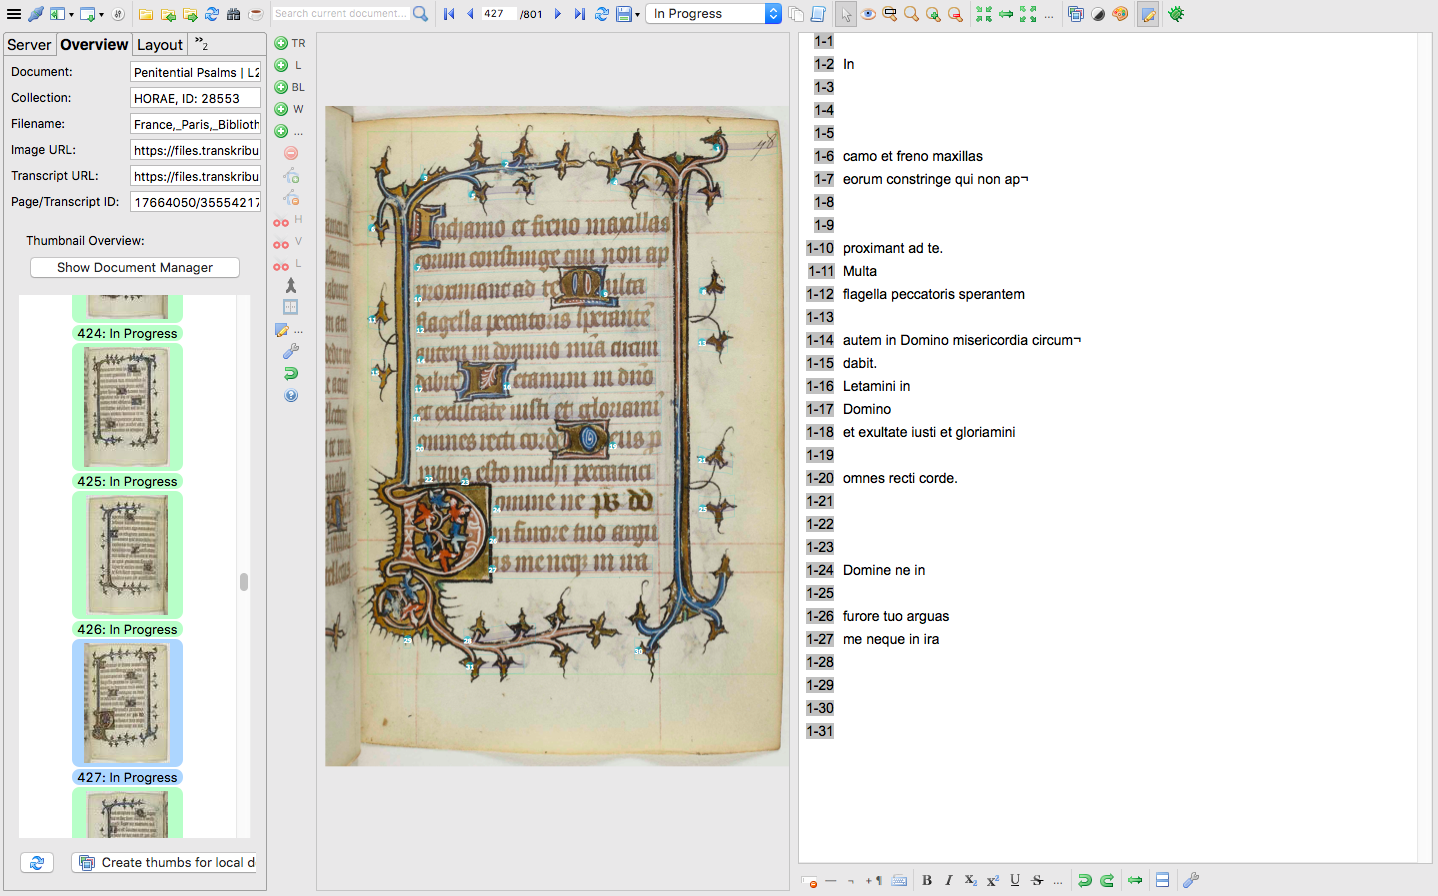
\includegraphics[width=13cm]{img/ML/psaumes_transkribus.png}

    \caption{Exemple d'un alignement d'un extrait de psaumes pénitentiels sur Transkribus, extrait du manuscrit ms. lat. 01403, f.78r, conservé à la Bibliothèque nationale de France.}
    \end{figure}

En ce qui concerne la création du modèle linguistique, prise en charge par le LS2N, il s'agit de faire apprendre plusieurs fois la Bible comme des textes différents à chaque fois, car les livres d'heures, comme les livres liturgiques de manière générale, contiennent beaucoup de références bibliques. L'idée d'intégrer un dictionnaire de latin dans l'apprentissage a été discutée. En effet, le grand nombre d'abréviations et de variantes orthographiques dans les livres d'heures risque de gêner la détection des caractères si la langue latine est trop normalisée. Toutefois, fournir un texte sans langue détectée est absurde. La solution serait d'utiliser les méthodes du \textit{postprocessing}, afin que la machine soit capable de détecter les anomalies linguistiques, c'est-à-dire ce qui diffère de la langue normalisée. Le \textit{postprecessing}, traduit comme le \og post-traitement\fg{}, est une des composantes de la \textit{Knowledge Discovery in Databases}, soit la découverte de savoirs dans de larges bases de données\footcite[p. 1]{Postprocessing}. Cette découverte de savoirs est possible grâce à cinq étapes\footcite[p. 2]{Postprocessing} : 
\begin{enumerate}
    \item Déterminer les contours de la problématique, spécifier le but de la découverte afin de choisir le domaine d'application le plus pertinent.
    \item Formaliser la représentation de l'objet et collecter les données selon cette représentation.
    \item Les données étant souvent incomplètes ou \og bruitées\fg{}\footnote{Dans le domaine des données, le bruit désigne un surplus d'informations inutiles dans le cadre des objectifs déterminés.}, en somme imparfaites, il est important de les structurer et de les ordonner pour qu'elles deviennent exploitables. Ce travail est appelé \og \textit{preprocessing}\fg{}.
    \item Vient ensuite l'étape du \textit{data mining} pour donner du sens aux données, à l'aide de méthodes statistiques, de réseaux de neurones et d'algorithmes.
    \item le \textit{postprocessing} constitue la dernière étape, qui consiste à vérifier la cohérence des traitements effectués, et au besoin, adapter le modèle existant pour diminuer le taux d'erreurs. Le savoir peut alors être interprété et intégré dans celui existant. 
\end{enumerate}

Il faut ici rappeler que l'enjeu de ce processus n'est pas d'améliorer la transcription du texte, mais sa détection. On peut ensuite identifier les termes de référence pour le plagiat, grâce à un repérage des similarités entre les phrases. \\

Il est maintenant intéressant de voir dans quelle mesure le protocole d'annotation et l'établissement de la vérité terrain ont servi la reconnaissance automatique d'images et de textes dans les livres d'heures. Contrairement à la reconnaissance de l'écriture imprimée (\textit{Optical Character Recognition}) où les modèles peuvent être harmonisés, la reconnaissance d'écriture manuscrite (\textit{Handwritten Text Recognition}) représente un enjeu en ce qu'elle implique des modèles spécifiques au type de documents traités. Cela est d'autant plus vrai pour les écritures médiévales, dans une langue éloignée de la nôtre, et offrant des spécificités en terme de formes des lettres et d'usage d'abréviations\footcite[p. 21]{Seg_Livres_Heures}. Le type d'écriture peut également varié selon l'époque et la zone de provenance du manuscrit. Il faut donc constituer un corpus d'écritures relativement homogènes pour donner plus de pertinence au modèle d'entraînement\footnote{Que l'on songe à la classification de Lieftinck-Gumbert-Derolez, qui distingue plusieurs variantes au sein des écritures gotiques, de la \textit{textualis} à l'\textit{hybrida} en passant par la \textit{cursiva}. Cf. \cite{classification_ecriture_gothique}.}.


	\subsection{Analyser la structure des pages}
	
	Avant de s'intéresser plus précisément à la reconnaissance textuelle, il est important d'entraîner le modèle sur la structuration des pages, afin qu'il distingue celles qui contiennent du texte à analyser de celles qui n'en contiennent pas\footnote{Cette étape d'analyse de la mise en page est communément appelée \textit{Document Layout Analysis}.}. Quel est l'état de l'art des systèmes de détections de lignes de texte, de zones dans une page de manuscrit ou d'incunable et de leur typologie ? Pour pouvoir procéder automatiquement sur un large panel de collections de livres d'heures hétérogènes, il est indispensable de créer un jeu de données annoté de pages représentatives de la variété des typologies et des présentations\footcite[p. 7]{annotated_dataset_book_hours}. On peut ici rappeler que le corpus dépasse les 500 manuscrits numérisés, disponibles pour la plupart via la BVMM\footnote{Bibliothèque Virtuelle des Manuscrits Médiévaux.} et Gallica, tous deux sous la responsabilité de l'IRHT et de la BnF. Le tableau ci-dessous permet d'avoir une idée de l'ampleur et de la provenance des données à annoter automatiquement : 

	\begin{figure}[!h]
    \centering
    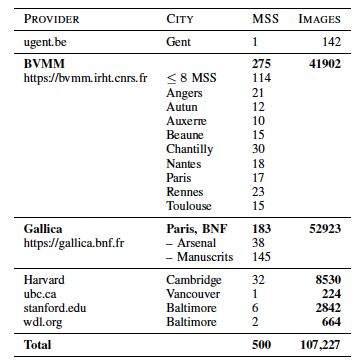
\includegraphics[width=10cm]{img/ML/provenance_dataset_annotated.png}
    \caption{Nombre et provenance des images et manuscrits du jeu de données. Cf. \cite[p. 8]{annotated_dataset_book_hours}}
    \end{figure}
    \clearpage
    
    L'objectif est donc de traiter ce jeu de données grâce au \textit{machine learning}, d'où le besoin de pages annotées par des experts pour entraîner le modèle. Des images de reliures ou de folios blancs ont également été incluses dans le corpus afin de faire détecter à la machine ce qui contient du texte de ce qui n'en contient pas. Pour rappel, le \textit{machine learning} désigne un système permettant de découvrir des répétitions, des similarités dans un ou plusieurs flux de données, et de construire des prédictions à partir de statistiques. Les premiers algorithmes d'apprentissage automatique ont été conçus dès les années 1950\footnote{Le plus célèbre est le Perceptron, mis au point par Frank Rosenblatt en 1957. Il s'agit d'un classifier linéaire qui consiste à classer ensemble des échantillons qui ont des propriétés communes, et de séparer ceux qui se différencient.}.
    
    Le \textit{machine learning} représente alors une branche de l'intelligence artificielle, mais ne peut être confondu avec cette dernière. L'intelligence artificielle désigne en effet ce qui permet à la machine d'apprendre et de comprendre des concepts en faisant des liens entre les données, en s'inspirant du système neuronal humain. L'intelligence artificielle s'appuie donc ici sur des statistiques et la création de probabilité à partir d'un jeu de données précis, afin qu'à partir d'une forme, le modèle soit capable de déduire de quelle section de page, lettre, mot, ou phrase il peut s'agir. Quant au \textit{deep learning}, il participe à l'intelligence artificielle en ce qu'il permet à la machine d'apprendre par elle-même au fur et à mesure qu'on lui fournit des données de qualité, sans avoir besoin d'être entraînée, mais il ne recouvre pas l'ensemble des techniques inhérentes à l'intelligence artificielle\footcite{Automatisation_ML}. \\
    
    \begin{figure}[!h]
    \centering
    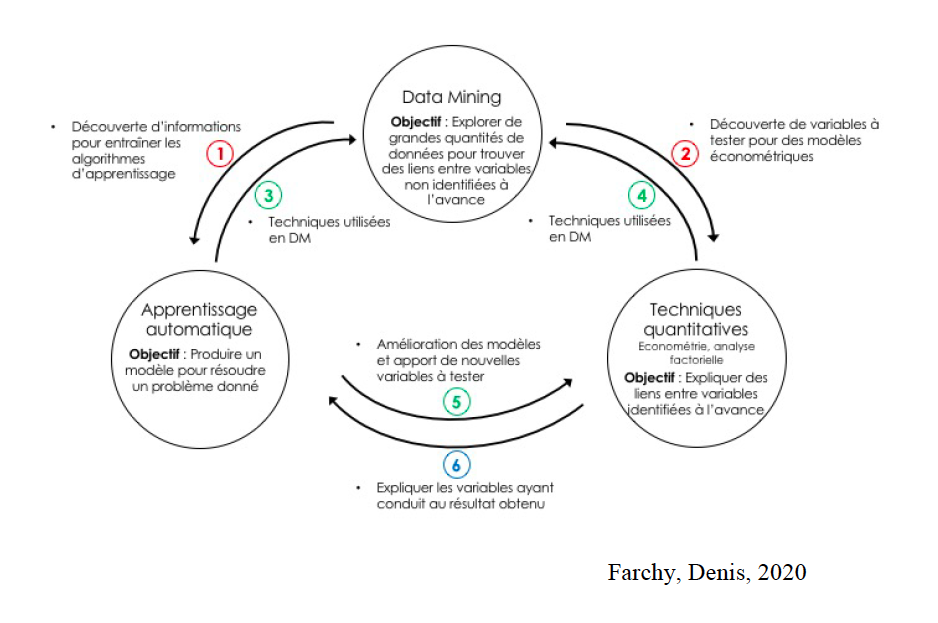
\includegraphics[width=13cm]{img/ML/liens_analyse_donnees.png}
    \caption{Schéma des liens entre les diverses approches d'analyse des données. Cf. \cite[p. 13]{Mission_IA_et_Culture}}
    \end{figure}
    
    En ce qui concerne la classification automatique des images de livres d'heures, elles ont été classées à partir des classes définies ci-dessous à partir d'un réseau de neurones d'apprentissage profond \footnote{Les classes de subdivision d'une page sont documentées dans le cadre du projet à l'adresse suivante : \url{https://gitlab.com/mlbonhomme/arkindex_annotation/-/tree/master/HORAE}.} :
	\begin{itemize}
	    \item \textit{page}\footnote{Si une image présente une double page, il est important d'annoter chaque page individuellement.}.
	    \item \textit{decorated\_border} et \textit{illustrated\_border} pour les bordures ; la première catégorie concerne les bordures avec des ornementations sans signification particulière (par exemple les motifs floraux ou végétaux), tandis que la deuxième se réfère aux illustrations signifiantes (scènes inspirées du texte biblique par exemple).
	    \item \textit{miniature}.
	    \item \textit{text} pour les zones de textes sur la page, donc si une page est divisée en deux colonnes, deux zones de texte sont annotées.
	    \item \textit{border\_text} pour le texte en marge dans les bordures.
	    \item Les initiales peuvent être annotées avec trois classes, \textit{decorated\_initial} pour les initiales ornées, \textit{simple\_initial} pour les initiales sans décoration particulière, seulement un peu plus épaisses que le reste du texte, \textit{historiated\_initial} pour les initiales historiées. 
	    \item Les autres éléments décoratifs sont répartis entre \textit{line\_filler}, soit les fins de ligne ornementées, ou bien \textit{ornament} pour les décorations à l'intérieur du texte qui ne sont pas des miniatures ; il peut s'agir des notations musicales.
	    \item la classe \textit{text\_line} définit les zones de texte ligne par ligne.
	\end{itemize}
	
	\begin{figure}[!h]
    \centering
    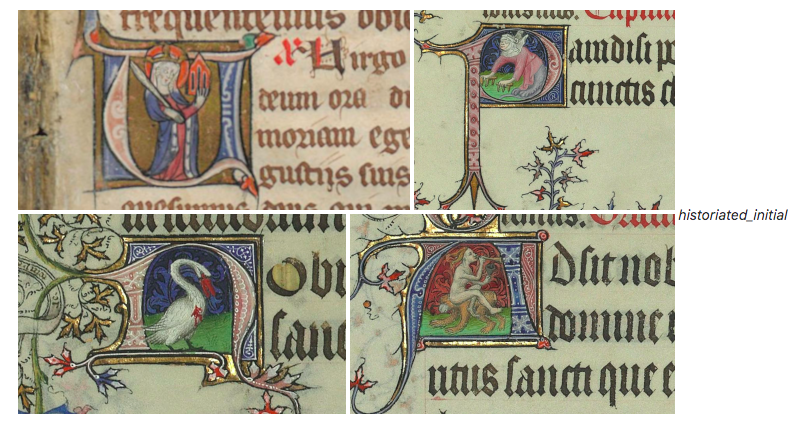
\includegraphics[width=10cm]{img/ML/historiated_initial.png}
    \caption{Exemple d'initiales à annoter avec la classe \textit{historiated\_initial}}
    \end{figure}
    
    \begin{figure}[!h]
    \centering
    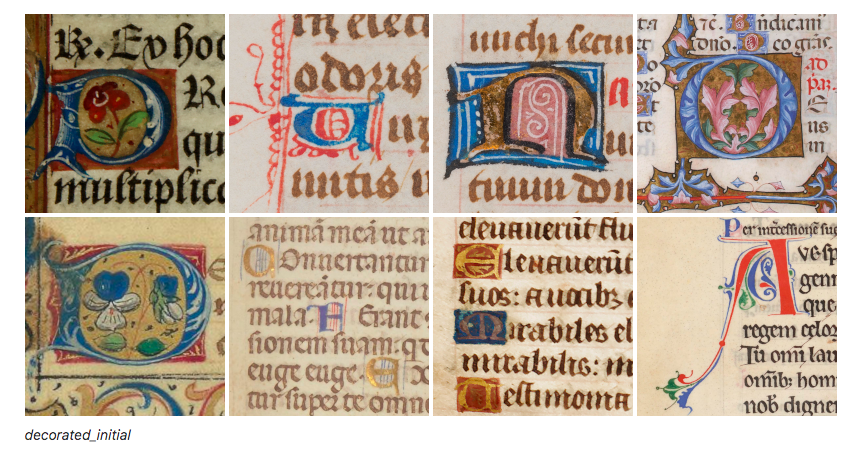
\includegraphics[width=10cm]{img/ML/decorated_initial.png}
    \caption{Exemple d'initiales à annoter avec la classe \textit{decorated\_initial}}
    \end{figure}
	
	\begin{figure}[!h]
    \centering
    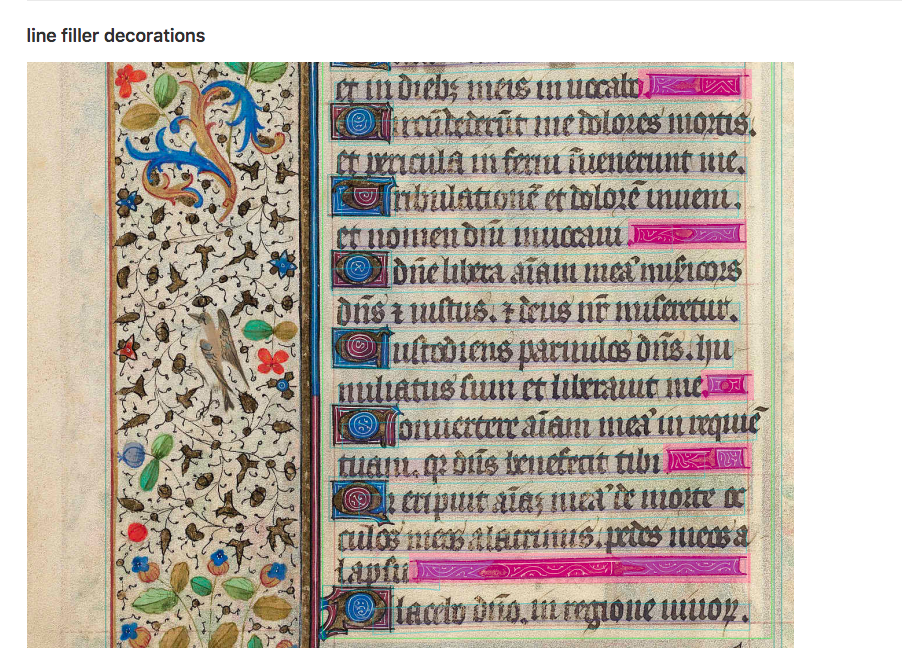
\includegraphics[width=10cm]{img/ML/line_filler.png}
    \caption{Exemple d'élément décoratif avec la classe \textit{line\_filler}}
    \end{figure}
    
    Cette méthodologie appartient donc au domaine du \textit{deep learning}. Sous-domaine du \textit{machine learning}, il est constitué de réseaux de neurones convolutionnels profonds, à l'image du fonctionnement du cerveau humain\footcite[p. 68-69]{deep_convolutional_neural_networks}. Les successions de neurones prennent en entrée les sorties des couches de neurones précédentes, afin que la machine apprenne d'elle-même. Les premières approches en \textit{deep learning} datent des années 1980, avec la mise au point d'un type d'algorithme appelé \textit{Convolutional neural network}\footcite[p. 1-3]{deep_convolutional_neural_networks}. Pour être efficace, l'apprentissage profond doit donc fonctionner avec un volume de données bien plus considérable que les réseaux de \textit{machine learning}, ce qui lui permet de réaliser des tâches plus complexes et plus précises.
    
    Une fois les pages classifiées automatiquement, la deuxième étape consiste à les regrouper selon leurs ressemblances. L'objectif est ainsi de détecter les pages qui sortent du lot, qui présentent un agencement suffisamment rare pour former un groupe à part\footcite[p. 8]{annotated_dataset_book_hours}. À partir de cette détection, un échantillon de pages à annoter a été sélectionné afin de représenter dans l'apprentissage la diversité des mises en page. Parmi les 600 images de l'échantillon, 141 correspondent aux dispositions les plus fréquentes, et 459 aux dispositions les plus rares et variées\footcite[p. 8]{annotated_dataset_book_hours}. 
    
    Le processus d'annotation s'est ensuite effectué grâce au logiciel Transkribus, développé dans le cadre du projet européen READ\footnote{Cf. \url{https://read.transkribus.eu/e-learning/}.}. Si une partie des classes doit être annotée manuellement afin d'établir une vérité terrain, les \textit{text lines} et les \textit{text regions} sont annotées automatiquement par Transkribus, bien qu'une vérification s'impose. En effet, le logiciel peut être sensible à la couleur de l’encre et donc mal distinguer les lignes si cette couleur est semblable à celle du parchemin. La vérité terrain est ici déterminée grâce à un corpus inter-annotateur de 10 images, où chaque annotateur travaille sur le même corpus, afin de mesurer les éventuels écarts et désaccords dans l'annotation, mais aussi de voir ce qui fait consensus. \\
    
    Au vu de la variété des classes et des pages, il a fallu choisir un outil d'analyse automatique flexible mais aussi capable d'uniformisation. C'est alors le réseau \textit{dhSegment} qui a été adopté, car cet outil a fait preuve de résultats satisfaisants pour le traitement de documents historiques. Il présente notamment les avantages de travailler avec une petite quantité de données d'entraînement, et de réaliser des opérations variées, comme l'extraction de lignes et l'analyse de la mise en page\footcite[p. 9]{annotated_dataset_book_hours}. En s'appuyant sur les réseaux de neurones, \textit{dhSegment} propose des solutions pour découper une page de manuscrit, extraire des enluminures du texte, localiser le texte dans une image numérisée, entre autres choses. Ces problématiques étaient traitées à l'aide de méthodes de segmentation disparates et hétérogènes, s'appliquant à des typologies de documents précises\footcite[p. 1]{deep_learning_segmentation}. 
    
    Utilisant l'outil d'apprentissage automatique \textit{TensorFlow}, notamment employé pour la détection d'objets, la segmentation se fait en deux étapes. La première s'appuie sur les réseaux de neurones convolutionnels qui prennent une image du document en entrée et rendent en sortie une cartographie des probabilités des caractéristiques prédictives attribuées à chaque pixel. La deuxième étape consiste à transformer les prédictions en la sortie souhaitée pour la tâche à effectuer\footcite[p. 1-2]{deep_learning_segmentation}. 
    
    \begin{figure}[!h]
    \centering
    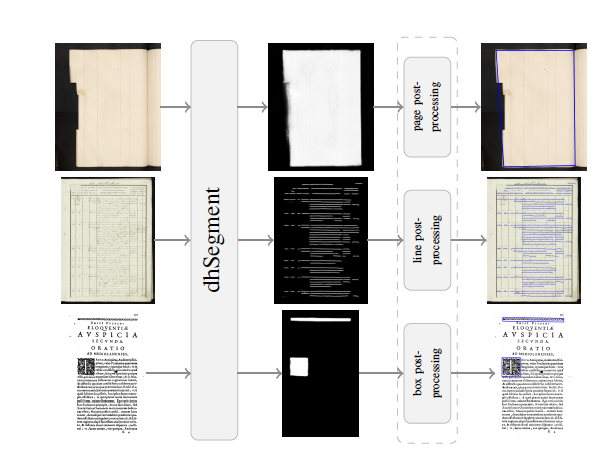
\includegraphics[width=13cm]{img/ML/etapes_dhSegment.png}
    \caption{La méthode de segmentation \textit{dhSegment} développée par Sofia Ares Oliveira et Benoît Seguin. Cf. \cite[p. 2]{deep_learning_segmentation}}
    \end{figure}
    
    L'intérêt de cette méthode est de limiter les tâches de la deuxième étape relative au post-traitement à de simples opérations de prédiction. La première consiste à établir des critères selon les classes à trouver, afin que les prédictions divisent le corpus selon les classes à trouver. La deuxième opération relève de considérations morphologiques afin d'analyser les structures géométriques du document. Les deux dernières étapes recouvrent l'analyse des composants connectés, afin de filtrer ceux qui resteraient après les deux premières étapes, puis la vectorisation, technique pour que plusieurs opérations soient traitées simultanément, afin que les zones détectées soient rassemblées en un ensemble de coordonnées\footcite[p. 2]{deep_learning_segmentation}. En adaptant ces critères au cas souhaité, on peut entraîner le corpus. Les résultats de la première expérimentation du \textit{dhSegment} témoignent de la possibilité pour un outil construit à partir de l'architecture générique du \textit{deep learning} de s'appliquer à des tâches de segmentation spécifiques tout en utilisant un processus standardisé. Cela signifie que des bouts de programmation peuvent être entraînés par des non-spécialistes, et être efficients pour de documents divers et variés\footcite[p. 6]{deep_learning_segmentation}. 
    
    Dans le cadre du jeu de données composé de livres d'heures, les résultats de cette méthode sont globalement satisfaisants, mais peuvent être améliorés. En effet, l'indice d'\textit{Intersection-over-Union}, soit le pourcentage de recouvrement de la zone établie par la vérité terrain par la zone de prédiction détectée automatiquement est entre 80\% et 90\% pour les lignes de texte et entre 60\% et 80\% pour l'agencement de la page\footnote{Le pourcentage varie selon la taille de la page d'entrée, cf.\cite[p. 10]{annotated_dataset_book_hours}.}. Les données bénéficieraient donc à être traitées avec un réseau de neurones plus complexe. \\
    
    Une des prochaines étapes concerne la reconnaissance des couleurs. Il faudrait alors entraîner le modèle avec les class \og \textit{red}\fg{}, \og \textit{blue}\fg{}, \og \textit{gold}\fg{} et \og \textit{green}\fg{} et analyser la variation de pixels au sein d’un même manuscrit. Cela serait intéressant pour avoir par exemple une vision du pourcentage de rubriques dans les livres d'heures. Toutefois, ce processus exclut les manuscrits numérisés en noir et blanc. \\
    
    Une des parties richement colorées est justement celle formée du calendrier.
    
    
    \subsection{Le cas spécifique des calendriers}
    
    Au cours de la réflexion sur la classification des pages, la classe \textit{Calendar} a été ajoutée pour les calendriers. En effet, si l’on annote ligne par ligne la structure tabulaire des calendriers, on perd l’intelligence des données. Les pages contenant des calendriers répondent ainsi à une structuration spécifique et à une typologie précise, et leur analyse dans le cadre des livres d'heures est précieuse pour comprendre les types d'usages et de dévotions auxquels nous sommes confrontés. Un calendrier peut ainsi mentionner des fêtes et des saints donnant des indications à la fois sur la période dans laquelle il a été composé (un saint peut avoir été récemment canonisé), comme sur sa destination (avec la mention d'un saint local par exemple)\footcite[p. 767]{analyse_calendrier}. Riche en informations, les calendriers contiennent généralement les éléments suivants : 
    \begin{itemize}
        \item les calendes indiquent le premier jour de chaque mois ;
        \item les nones indiquent le 5 du mois, sauf pour les mois de mars, mai, juillet et octobre où elles indiquent le septième jour du mois ;
        \item les ides indiquent les 13 du mois, sauf pour mois de mars, mai, juillet et octobre où elles sont placées au 15 du mois ;
        \item le nombre d'or, sous la forme de chiffre romain inscrit à gauche en face de certains jours\footnote{Ce chiffre indique les nouvelles lunes pour le calcul du cycle métonique, soit une période d'environ 19 ans où les cycles lunaires et solaires s'alignent.} ;
        \item la \textit{littera dominicalis}, la lettre indiquant le dimanche, renouvelée tous les ans\footnote{Chaque jour de la semaine est ainsi associé à une lettre, de A à G} ;
        \item le \textit{terminus}, soit la dernière date possible pour une fête mobile ;
        \item l'indication \textit{claves pasche}, qui détermine le jour à partir duquel on commence le décompte pour la date de Pâques, dépendant elle-même du cycle métonique.
    \end{itemize}
    
    On peut également y trouver d'autres indications d'ordre astronomique, avec les nombres d'heures de jour et de nuit dans un mois, la mention des équinoxes ou des embolismes\footnote{Il s'agit du nombre de jours de différence entre l'année solaire et l'année lunaire.} mais aussi l'indication de jours considérés comme néfastes pour certaines activités\footnote{Ce jours peuvent être signalés par un \og D\fg{} à droite dans la marge.}, les signes du zodiaque ou des indications sur les activités du mois. L'analyse d'un grand nombre de calendriers, de leurs points communs ou de leur différences selon les époques, permet ainsi de mieux visualiser l'émergence de nouveaux cultes comme leur propagation\footcite[p. 768]{analyse_calendrier}. \\
    
    À cet égard, une base de données relationnelle d'après les travaux de Aaron Macks rassemble un corpus de calendriers de livres d’heures. Il s'agit du site \textit{CoKL: Corpus Kalendarium}\footnote{Cf. \url{http://www.cokldb.org/}.}. Il est ainsi possible d'y faire des recherches par noms de saints ou par dates de fêtes et de voir dans quels livres d’heures ils sont mentionnés. On peut également comparer les calendriers de divers manuscrits en mettant en regard les usages, les langues, la foliotation, ou encore les transcriptions de calendriers.
    
    \begin{figure}[!h]
    \centering
    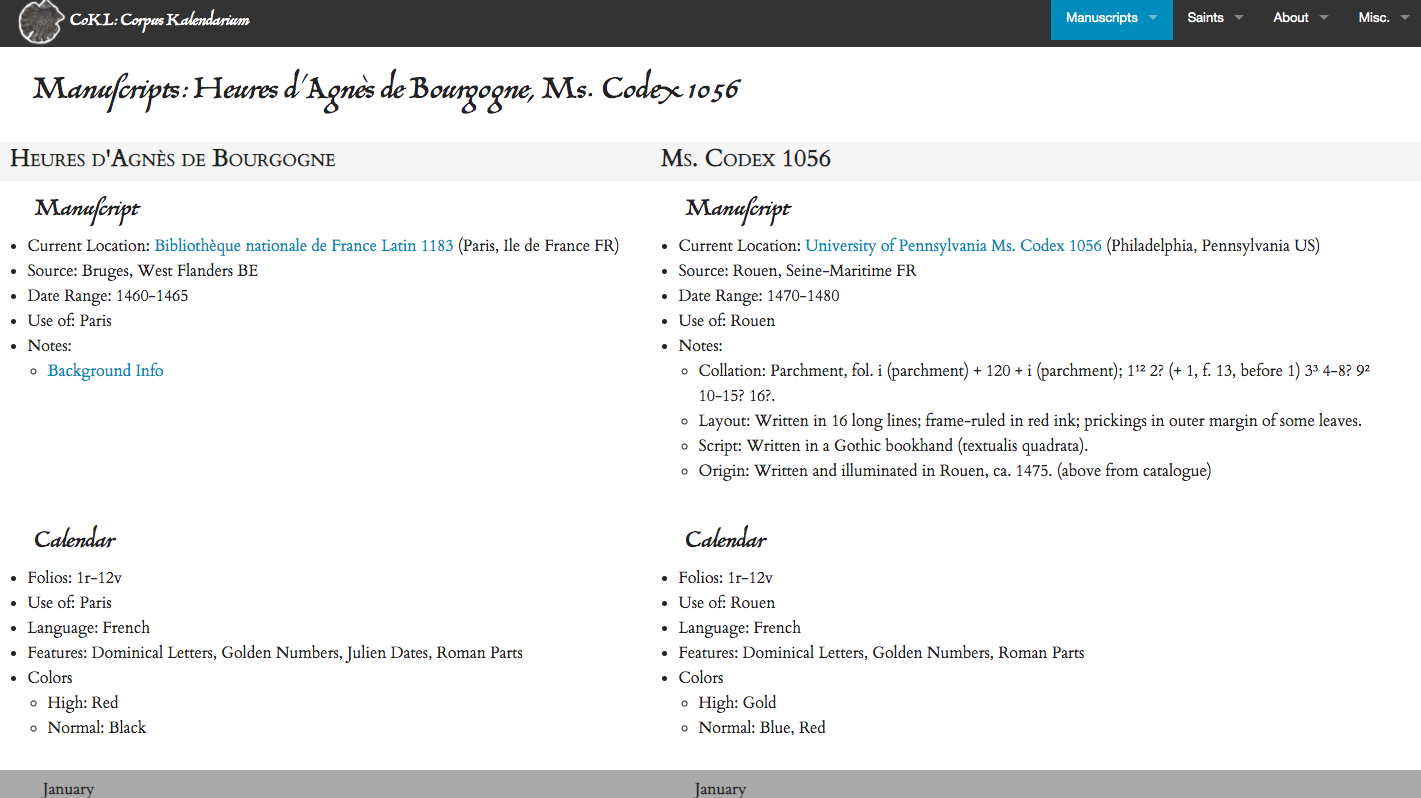
\includegraphics[width=13cm]{img/DataViz/CoKL1.png}
    \end{figure}
    
    \begin{figure}[!h]
    \centering
    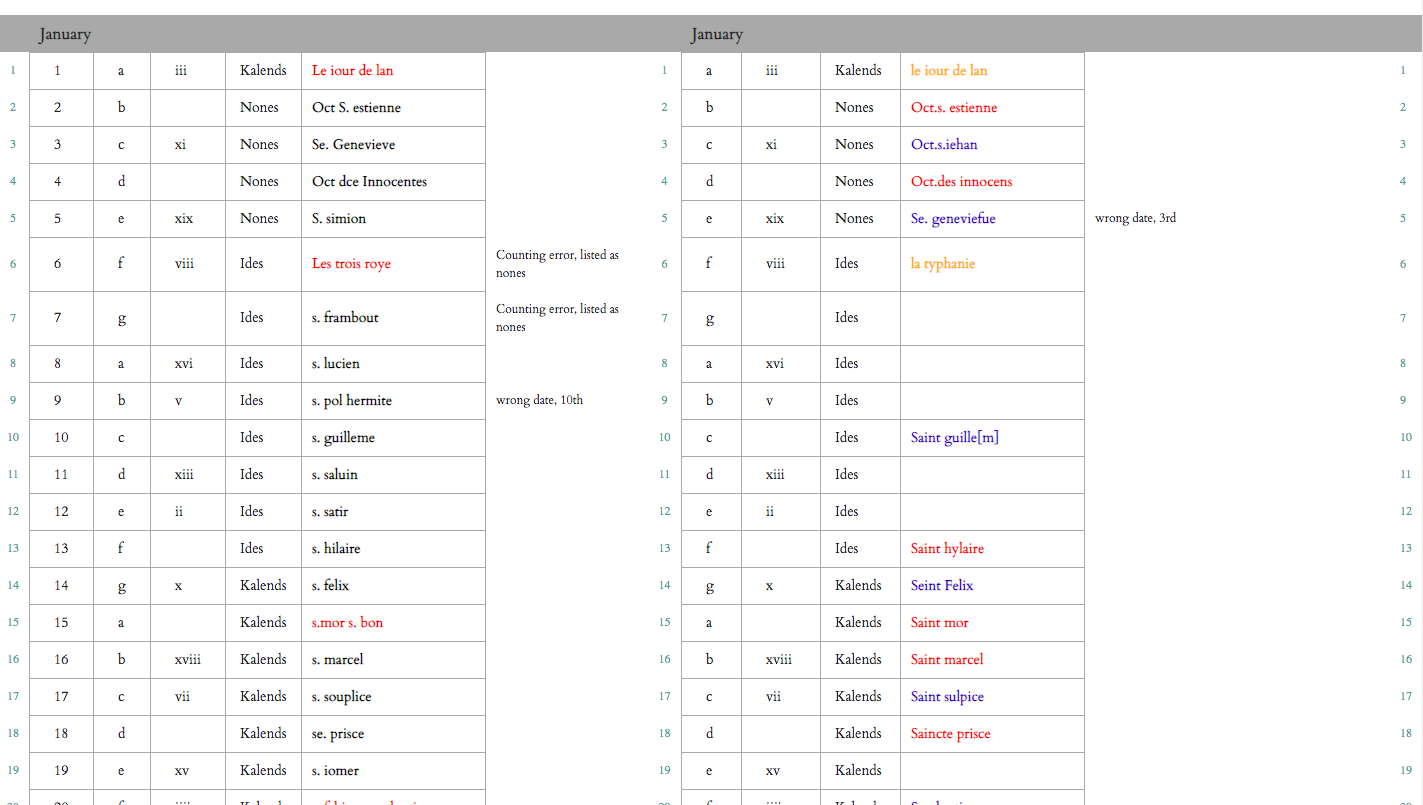
\includegraphics[width=13cm]{img/DataViz/CoKL2.png}
    \caption{Exemple de visualisation comparative de calendriers d'après la base de données relationnelle \textit{CoKL: Corpus Kalendarium}.}
    \end{figure}
    
   Les pages contenant un calendrier mériteraient donc à être détectées avec leur spécificité, sous la forme d'une structuration tabulaire elle-même divisée en zones de texte. La détection de la structuration des pages et leur classification est ainsi un préliminaire indispensable à la reconnaissance automatique de caractères. 

	
	\subsection{Analyser le contenu textuel}
	
	Le projet HORAE met en avant des méthodes et traitements automatiques spécifiquement adaptés à la structure des livres d'heures. Ces méthodes utilisent l'approche de segmentation semi-supervisée afin de mieux retrouver leur structure malgré le bruit engendré par la reconnaissance d'écriture\footcite[p. 13]{Seg_Livres_Heures}. 
	
	Une fois les lignes de textes localisées dans chaque image contenant une classe de type \og page\fg{}, elles sont extraites afin que le système de reconnaissance d'écriture soit appliqué sur chaque imagette de la ligne. La reconnaissance d'écriture comprend alors deux étapes\footcite[p. 22]{Seg_Livres_Heures} : 
	\begin{enumerate}
	    \item l'application d'un modèle optique qui reconnaît des caractères, fragments de caractères ou de mots ;
	    \item l'application d'un modèle de langue qui détermine les séquences de caractères et de mots les plus vraisemblables.
	\end{enumerate}
	
	Pour la reconnaissance des caractères dans les livres d'heures, les membres du projet ont choisi d'utiliser la librairie logicielle KALDI\footnote{\textit{Kaldi Speech Recognition Toolkit}. La documentation et le code source sont disponibles à l'adresse suivante : \url{https://github.com/kaldi-asr/kaldi}.}. Grâce à la généralisation de l'utilisation de réseaux de neurones profonds, l'outil, initialement prévu pour la reconnaissance de la parole, est aisément adapatable à la reconnaissance d'écriture\footcite[p. 23]{Seg_Livres_Heures}. Grâce à Kaldi Horae Recognizer, on est capable de calculer le vocabulaire commun à la même section de plusieurs manuscrits. Ainsi, le 23 juillet dernier a été confirmé le fait que 40\% à 48\% du vocabulaire des 247 lignes transcrites de la prière \textit{Obsecro te} issue d'un corpus de dix manuscrits est commun à la Bible. \\
	
	Le système repose sur la combinaison de réseaux de neurones profonds d'une part, et de modèles de Markov cachés d'autre part. Si le fonctionnement des réseaux de neurones rejoint ce qui a été fait pour la détection des zones dans une image, un Modèle de Markov Caché (MMC) est un modèle statistique avec des paramètres inconnus. Il est un des premiers systèmes capables de transcrire complètement une image de mots ou de ligne\footcite[p. 66]{Reconnaissance_HTR_These}. À partir d'un état donné, le système calcule des probabilités de transition et de valeur de sortie. Ainsi, le modèle optique, capable de reconnaître des formes et d'en déduire des caractères, est composé de plusieurs couches de réseaux de neurones convolutionnés ainsi que de couches TDNN\footnote{\textit{Time Delay Neural Networks}.} pour modéliser les caractères en contexte. Les prédictions sont ensuite utilisées par le modèle HMM qui modélise les mots comme des séquences de caractères. Les séquences de mots sont alors modélisées par un modèle de langue statistique de type n-gramme\footcite[p. 24]{Seg_Livres_Heures}. Un n-gramme est une sous-séquence de \textit{n} éléments, qui prend la forme de caractères ou de mots, afin de définir l'ensemble des enchaînements de caractères ou de mots possibles\footcite[p. 66]{Reconnaissance_HTR_These}. À partir d'un corpus d'apprentissage, le modèle cherche les probabilités que la prochaine lettre soit telle lettre avec un historique de taille \textit{n}. Toutefois, ce modèle présente le risque de mener à des sur-représentations ou à des sous-représentations, car plus le pas \textit{n} est grand, plus le nombre d’éléments est grand, et plus on risque d’obtenir des enchaînements rares\footcite[p. 65]{Reconnaissance_HTR_These}.
	
	Le modèle a été entraîné à partir des corpus de manuscrits médiévaux formés dans le cadre de précédents projets, notamment ORIFLAMMS\footnote{\textit{Ontology Research, Image Features, Letterform Analysis on Multilingual Medieval Scripts}.} et ECMEN\footnote{\textit{Écriture Médiévale et outils Numériques}.}, constituant des corpus en latin et en ancien français. Dans le cadre d'HORAE, le modèle a été entraîné sur 247 lignes transcrites manuellement issues des \textit{Obsecro te} de huit livres d'heures du corpus cible. Si les taux d'erreurs mots (WER pour \textit{Word Error Rate}\footnote{Cette métrique permet de calculer le taux d'erreurs par mot, c'est-à-dire qu'elle indique le taux de mots mal reconnus en se calquant sur un texte de référence.}) et les taux d'erreurs caractères (CER pour \textit{Character Error Rate}\footnote{Cette métrique renvoie au taux d'erreurs par caractère, calculer sur le même principe que le WER.}) restent assez élevés, ils n'empêchent pas l'identification des textes\footcite[p. 25]{Seg_Livres_Heures}. \\
	
	\begin{comment}
	Nous allons nous intéresser en premier lieu aux métriques WER et CER. Le Word
Error Rate ainsi que le Caracters Error Rate, sont des métriques permettant de calculer le
taux d’erreur par mot ou par caractères. Habituellement utilisé lors de travaux concernant
la reconnaissance de la parole, le WER indique le taux de mots mal reconnu, en se basant
sur un texte de référence. L’objectif est donc d’atteindre le taux le plus bas possible. Il est
capable de signaler des mots substitués et des mots insérés, qui n’existent pas en réalité.
On l’applique donc aux traitement de type HTR ou OCR.
	\end{comment}
	
	En effet, la reconnaissance des écritures manuscrites sert dans le projet HORAE l'identification automatique des textes. Cette identification se fait par la segmentation de textes, qui recouvre trois tâches distinctes\footcite[p. 26]{Seg_Livres_Heures} : 
	\begin{itemize}
	    \item la segmentation thématique, où les segments sont homogènes ;
	    \item l'identification thématique, où des thèmes sont assignés aux segments ;
	    \item le suivi thématique, où sont établies des relations entre les thèmes des segments, notamment de nature hiérarchique.
	\end{itemize}
	
	Pour segmenter un texte et détecter les changements de thèmes, les principales approches utilisées reposent sur l'analyse lexicale ou le calcul de la cohésion lexicale\footcite[p. 27]{Seg_Livres_Heures}. Toutefois, jusqu'à présent, les segmentations de textes linéaires ou hiérarchiques se sont appliquées à des textes scientifiques, narratifs ou à des dialogues écrits et retranscrits. Il s'agit ici de segmenter un texte manuscrit dont la reconnaissance de l'écriture a présenté un certain taux d'erreurs\footcite[p. 28]{Seg_Livres_Heures}. C'est donc une approche semi-supervisée qui a été privilégiée, fondée sur une représentation des parties des livres d'heures par prolongement de mots. 
	
	L'approche semi-supervisée est une classe de techniques de l'apprentissage automatique qui s'appuie sur des données annotées et non annotées. Il constitue donc un entre-deux entre l'apprentissage supervisé, qui ne peut se faire qu'à partir d'un ensemble de données annotées, ce qui demande un travail humain indispensable pour préparer les données, et l'apprentissage non-supervisé, ne se nourrissant que de données non annotées, ce qui implique que la machine détecte par elle-même les structures sous-jacentes des données d'entrée. La particularité du projet HORAE est, non pas d'utiliser des similarités lexicales entre deux blocs d'un même document, mais entre le document et une base de références externes contenant les textes préalablement annotés. Il s'agit donc d'aligner les textes de référence des livres d'heures et les textes transcrits, découpés arbitrairement en blocs distincts\footcite[p. 29]{Seg_Livres_Heures}. 
	
	Par rapport à l'état de l'art dans les méthodes de segmentation, l'approche proposée est une de celles qui donnent les meilleurs résultats. En terme d'analyse lexicale, le LS2N nous apprend par exemple que 45\% à 50\% du contenu de la Bible est présent dans les 10 livres d’heures analysés issus du corpus inter-annotateur, sachant que, en moyenne, un tiers du livre d’heures est composé de psaumes. Cette approche semi-supervisée produit donc des résultats encourageants pour les deux premiers niveaux hiérarchiques, même à partir d'une transcription imparfaite. 
	
    \begin{figure}[!h]
    \centering
    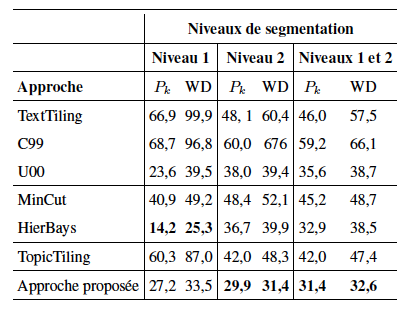
\includegraphics[width=10cm]{img/ML/Niveau_Segmentation.png}
    \caption{Analyse des différentes méthodes de segmentation pour les niveaux 1 et 2 de deux livres d'heures, dont l'un a une transcription imparfaite. P\textsubscript{k} et WD indiquent les taux d'erreurs. Cf. \cite[p. 32]{Seg_Livres_Heures}}
    \end{figure}
    
    Lors des réunions entre les partenaires, des pistes sont abordées pour améliorer l'HTR. Par exemple, si les lignes sont globalement courtes dans les livres d’heures\footnote{On estime la longueur des lignes de livres d'heures à moins de sept mots par ligne en moyenne.}, cela s'explique par sa position de manuscrit de luxe pour les gens non-spécialistes de la lecture. Les scribes évitent donc de couper les mots. Toutefois, si la situation se rencontre, il faut penser à fusionner les fins de lignes et les débuts de lignes pour améliorer la reconnaissance de vocabulaire. \\
    
    Que nous apporte, d'un point de vue historique et anthropologique, la reconnaissance automatique d'écritures et de textes d'un large corpus de livres d'heures ?

	
	\subsection{Des données structurées en masse : quand le numérique sert les humanités}
	
	Il s'agit de contextualiser et de saisir le caractère heuristique de l'utilisation des technologies numériques dans l'étude des livres d'heures, et au-delà, des pratiques dévotionnelles intimes des populations occidentales du Moyen Âge tardif. En effet, la constitution d'un corpus de livres d'heures pour l'annotation atteignant 794 livres, numérisés et segmentés, apporte des possibilités d'analyses et d'interprétations nouvelles. Ces livres sont conservés en France, en Suisse, en Allemagne, aux États-Unis, au Canada, en Grande-Bretagne, au Vatican ou en Belgique, dans des bibliothèques, des services d’archives ou encore des musées.\\
	
	L'analyse textuelle d'un grand nombre de livres d'heures permet en premier lieu de cerner leur composition, avec les grandes tendances que l'on retrouve quasi systématiquement et les variations, qui peuvent témoigner d'usages et de dévotions particuliers, propres à un temps donné, à une région géographique ou tout simplement à un intérêt personnel pour tel ordre religieux, tel saint, etc. Si chaque livre d'heures correspond à l'usage d'un diocèse, il s'inspire des grandes dévotions catholiques, celles de la Vierge Marie, de la Croix, du Saint-Esprit, ainsi que du culte des saints et des morts\footcite[p. VII-IX]{Leroquais_notices}. Plus la liste de manuscrits et incunables analysés automatiquement s'agrandit, plus la liste des classes au sein des différents niveaux hiérarchiques de l'annotation s'affine. Cela est particulièrement visible pour la liste des suffrages, dont on compte jusqu'à présent environ 191 classes différentes\footnote{Une liste de ces classes propres aux suffrages est disponible en annexes section \ref{annotation}.}. 
	
	Les suffrages sont composés d'une antienne, d'un verset et d'une oraison. Ils sont récités après les vêpres ou les laudes, en l'honneur de Dieu ou de saints. De manière générale, ils débutent par la sainte Trinité, puis viennent dans un ordre hiérarchisé la sainte Vierge, saint Michel, saint Jean-Baptiste, les apôtres, les martyrs, les confesseurs et les saintes. On peut ainsi y détecter les saints les plus invoqués au Moyen Âge, particulièrement contre les maladies d'après Victor Leroquais. Si leur ordre d'apparition par catégories est commun, le choix des saints célébrés varie. Cet indice de dévotions particulières interroge sur la ou les personne(s) à l'origine du choix des saints vénérés : s'agit-il de l'éditeur ? Du copiste ? D'une entente entre le transcripteur et le miniaturiste ? Du chef d'atelier ? Du destinataire du livre d'heures \footcite[p. XXI-XXII]{Leroquais_notices}? 
	
	Toujours d'après le chanoine Leroquais, l'une des parties les plus révélatrices du livre d'heures sont les prières\footnote{Les listes des messes et offices votifs découverts dans les livres d'heures du corpus sont disponibles en annexes, section \ref{annotation}.}. En effet, d'ordre privé et extra-liturgique, elle est \og celle qui a jailli spontanément de l’âme populaire, qui a traduit à un moment donné ses besoins et ses aspirations\fg{}\footcite[p. XXIX]{Leroquais_notices}. Elles représentent une communication immédiate avec Dieu ou les saints. Du point de vue de leur analyse, il serait intéressant de constater la part des prières en latin et en langues vernaculaires, ainsi que leur date approximative selon leurs formules. Si la plupart sont d'auteurs anonymes, les auteurs mentionnés font souvent plus figures d'autorité que de figures historiques véridiques\footcite[p. XXIX]{Leroquais_notices}. Au-delà du potentiel choix du destinataire, la comparaison entre ces prières, leur fréquence au sein des livres d'heures, permet de mesurer des tendances au sein de la piété populaire\footcite[p. XXX]{Leroquais_notices}. 
	
	La question des usages liturgiques est particulièrement complexe dans les livres d'heures. On trouve par exemple plus de 200 versions différentes du petit office de la Vierge dans les livres d'heures conservés à la BnF et observés par Leroquais\footcite[p. XXXVI]{Leroquais_notices}. Contrairement aux autres livres liturgiques, l'usage des offices ne reflète pas nécessairement le lieu de production et de destination, d'autant plus que les usages de Rome et de Paris sont les plus répandus. Les usages présents dans les livres d'heures, parfois différents d'une pièce à l'autre au sein d'un même manuscrit, peuvent s'inscrire dans des usages d'origine monastique, d'ordres religieux réguliers et séculiers. Parmi ceux observés par Victor Leroquais se trouvent : 
	\begin{itemize}
		\item l'ordre de Cluny, ordre monastique fondé en 910 ;
		\item les Chartreux, ordre monastique fondé en 1082 par Bruno de Cologne ;
	    \item les Cisterciens, ordre monastique fondé en 1098 par Robert de Molesme ;
	    \item les Guillelmites, ordre monastique fondé au \textsc{XII}\up{e} siècle par Guillaume de Maleval ;
	    \item les Prémontrés, ordre de chanoines réguliers fondé au \textsc{XII}\up{e} siècle par saint Norbert ;
	    \item Les Franciscains, ordre mendiant mineur fondé en 1210 par François d’Assise ;
	    \item Les Dominicains, ordre mendiant fondé en 1215 par Dominique Guzman ;
	    \item les Ermites de saint Augustin, ordre mendiant fondé en 1243 ;
	    \item les Célestins, ordre bénédictin fondé en 1248 par Pierre de Morrone, futur Pape Célestin V ;
	\end{itemize}
	
	Les usages de ces différents ordres se distinguent par des célébrations importantes de saints particuliers, notamment celui portant le nom du fondateur, étant parfois devenu lui-même un saint - ce qui par ailleurs est un bon indicateur pour la datation du manuscrit, selon la date de canonisation du fondateur, mais aussi pour les jours de dédicaces des édifices religieux ou de la réception de reliques, la \textit{translatio}\footnote{Ces réflexions sont inspirées d'une formation continue de l'École des Chartes, \og Les livres liturgiques manuscrits et imprimés : principes de catalogage\fg{}, donnée par Laura Albiero du 2 au 4 septembre 2020.}.\\
	
	Toutefois, l'utilisation de données entièrement numériques peut aussi limiter l'étude de certains aspects, notamment codicologiques. Par exemple, si l'on peut voir les réclames\footnote{\og Indication des premiers mots de la page suivante inscrite au bas d'une page, le plus souvent à la jonction entre deux cahiers, permettant de contrôler la bonne succession des feuillets ou cahiers.\fg{}.\cite{dico_codicologie}.} sur les pages numérisées, il est plus délicat de faire de la collation\footnote{Technique consistant à calculer le nombre de feuillets ou de cahiers que comporte un volume.}, car cela demande une approche physique pour mieux se rendre compte de certains paramètres. 
	
	En effet, dans le cas des livres d'heures, une approche anthropologique qui étudie le livre avant tout sous l'angle de son statut matériel d'objet peut se révéler particulièrement pertinente, d'autant plus pour ce type d'objet relevant du quotidien et de l'intimité. Restitué dans son contexte, l'objet apparaît comme un moyen d'influence des pensées et des actions, notamment dans l'expression de pratiques dévotionnelles et de cultes\footcite[p. 262]{Art_Agency}. Les livres d'heures constituent par ailleurs des objets en mouvement et en métamorphose, qu'ils soient remaniés pour l'ajout d'un saint récemment canonisé, ou bien amputés de feuillets enluminés, comme nous l'avons vu dans les travaux de Kathryn M. Rudy\footcite{Piety_in_Pieces}.
	
	Un autre aspect des livres d'heures pourrait être étudié, si les avancées en reconnaissance automatique de caractères le permet : la musique. Si les livres liturgiques sont indissociables du chant, et donc riches en notations musicales, il faut toutefois rappeler que cela est plus rare dans les livres d'heures\footcite[p. 57]{Music_Livre_Heures}. L'identification de traditions mélodiques peut ainsi être un indice de plus pour identifier la diffusion d'usages particuliers, tout comme la notation musicale peut indiquer une datation et une provenance géographique plus précise du livre\footnote{Parmi les différents types de notations, on distingue notamment la notation neumatique, dont une des plus anciennes apparaît dès le \textsc{IX}\up{e} siècle, \textit{in campo aperto} ou sur ligne, et la notation carrée, se développant principalement au \textsc{XII}\up{e} siècle en France.}. \\
	
	L'usage du numérique dans les SHS est de plus en plus prégnant. Xavier Darcos, chancelier de l'Institut de France, parle de \og déplacement des frontières\fg{}\footcite[p. 3]{recherche_HN}, à la fois car le numérique encourage la transdisciplinarité, mais aussi parce que le double enjeu des découvertes scientifiques et de l'amélioration des possibilités techniques se nouent. Il renouvelle également l'accès de tous au patrimoine. Il est vrai que la recherche, l'histoire médiévale en particulier, a toujours eu des rapports étroits avec l'ordinateur, que l'on songe à la revue \textit{Le Médiéviste et l'Ordinateur}, née en 1979. De plus, le \og tournant numérique\fg{} concerne l'ensemble des activités humaines, et pas que les humanités\footcite[p. 5]{recherche_HN}. Le projet HORAE s'inscrit donc dans cette mouvance qui fait du numérique à la fois un instrument de recherche, un outil de communication et un objet de recherche. L'utilisation de plus en plus sophistiquée du numérique dans les humanités a donné lieu au terme anglo-saxon \og \textit{digital humanities}\fg{}, terme popularisé avec la parution du livre \textit{A Companion to Digital Humanities}. D'après le \textit{Manifeste des digital humanities}, rédigé en 2010 à Paris, cosigné par plus de 250 chercheurs et 10 institutions,
	\begin{quote}
	    [...] les \textit{digital humanities} concernent l’ensemble des Sciences humaines et
sociales, des Arts et des Lettres. Les \textit{digital humanities} ne font pas table rase du passé.
Elles s’appuient, au contraire, sur l’ensemble des paradigmes, savoir-faire et
connaissances propres à ces disciplines, tout en mobilisant les outils et les
perspectives singulières du champ du numérique.
Les \textit{digital humanities} désignent une transdiscipline, porteuse des méthodes, des
dispositifs et des perspectives heuristiques liés au numérique dans le domaine des
sciences humaines et sociales\footcite[p. 7-8]{recherche_HN}.
	\end{quote}
	
	Pourtant, ce terme ne fait pas consensus. Certains acteurs du numérique au service du patrimoine culturel, comme Gautier Poupeau, ingénieur de la donnée à l'INA et chargé de cours dans le master \og Technologies numériques appliquées à l'histoire\fg{}, stipule que la nécessaire digitalisation des SHS rend le terme \og Humanités numériques\fg{} obsolète. Il compare la situation avec la physique ou la biologie, disciplines pour lesquelles l'usage du numérique n'a pas créé un mouvement revendicatif de l'usage du numérique dans les sciences. En faire une discipline à part restreindrait la place du numérique au lieu d'en faire une composante naturelle et intégrée au sein des différentes disciplines des sciences humaines et sociales\footcite{numerique_SHS}. 
	
	Dans un projet comme celui d'HORAE, où le champ des humanités numériques s'inscrit pleinement dans la recherche historique, chercheurs, ingénieurs, techniciens, \textit{data scientists}, s'unissent pour donner du sens à un flot de données, en l'occurrence les livres d'heures numérisés. En effet, l'approfondissement de leur étude, la possibilité de les lire avec des transcriptions, leur mise en relation et l'enrichissement des métadonnées les rendent bien plus visibles et accessibles qu'une simple numérisation de leur contenu\footnote{Sur les questions d'intelligibilité des données accessibles sur le web et le développement d'une compréhension partagée, cf. \cite[p. 38-60]{switching_codes}.}. \\
	
	Si le numérique a ses limites, et ne peut pas restituer l'émotion d'un contact physique humain avec l'objet étudié, les possibilités offertes par le \textit{machine learning} dans le traitement de données nombreuses est un gage de renouvellement de notre compréhension de la ré-appropriation des usages liturgiques dans les livres d'heures, ainsi que des réseaux de transmissions des livres, et donc des idées, croyances et cultes qu'ils diffusent.

	
	\chapter*{Conclusion}
	\addcontentsline{toc}{chapter}{Conclusion}
	
	Ainsi, les trois grandes étapes du stage exposées dans ce mémoire permettent de dresser un bilan des apports, limites et promesses offertes par le numérique dans l'étude des lives d'heures. 
	
	Le travail de structuration des métadonnées, plus précisément du catalogue de notices de livres d'heures élaboré par Victor Leroquais\footcite{Leroquais_notices}, permet la création d'une édition numérique normalisée et interopérable, selon les standards définis par TEI All, afin de faciliter l'échange et l'analyse d'informations. Il est désormais plus facile de répertorier et de comparer la présence de certains textes dans les livres d'heures conservés à la Bibliothèque nationale, de détecter leur structure, la place qu'occupent certaines pièces liturgiques, leurs usages. Le catalogue sous forme numérique donne une meilleure visibilité du contenu et des aspects codicologiques des livres d'heures tout en fournissant un apport pour les données numérisées amassées dans le cadre du projet. L'utilisation de langages de programmation participe à l'automatisation du processus d'encodage sur des centaines de notices, et constitue évidemment un gain de temps considérable. 
	
	Toutefois, l'automatisation reste perfectible, d'où l'intérêt de réfléchir à différentes possibilités, Les langages Python, XSLT ou l'exemple de GROBID pour l'apprentissage machine en l'occurrence, afin de choisir le programme le plus efficace. Différentes solutions peuvent parfois se compléter, comme l'utilisation des possibilités offertes par le logiciel Word, XSLT et XQuery dans notre cas. La mise en place du programme le plus efficace peut certes être chronophage, mais peut aussi s'avérer être un gain de temps pour la suite et éviter certains rattrapages manuels dans la structuration des métadonnées. Il peut être difficile de cerner ce qui est le plus efficace dans l'instant et ce qui le sera pour la suite. De plus, le numérique ne peut pas tout. L'étape de vérification de l'intégrité des données reste indispensable, afin de s'assurer de l'objectif principal, l'établissement de données de qualité pour la recherche en sciences humaines et sociales. \\
	
	La modélisation et l'import des données du cursus dans une base de données relationnelle s'avèrent essentiels pour la gestion et la visibilité d'un grand nombre de données reliées entre elles. Leur implémentation dans une base de données, dans le respect de leur cohérence, permet ainsi de mieux les visualiser et de produire des outils d'analyse. On peut penser à la génération de cartes sur la circulation des usages, des lieux de conservation des manuscrits du corpus, de graphes de liens entre les pièces et sections du livre d'heures selon les usages, etc. Les bases de données, relationnelles entre autres, sont un outil indispensable pour la manipulation et la visualisation des données. 
	
	L'étape de modélisation est alors cruciale pour comprendre l'objet à étudier, n'oublier aucun de ses aspects. Cette étape ne peut être négligée pour donner une forme complète et cohérente aux données dans la base. La difficulté est donc de créer un modèle reflétant la complexité de la réalité tout en pouvant être implémenté et mis à jour dans la base de données. Il faut ici souligner l'importance d'un logiciel ergonomique répondant aux besoins des différents projets de recherche, ainsi qu'un dialogue constant avec les techniciens en charge de la conception des bases de données utilisées. Dans le cadre d'HORAE, Heurist, base développée pour la TGIR\footnote{Très Grande Infrastructure de Recherche.} Huma-Num, a ainsi pour objectif de donner accès à une interface simple d'utilisation sans avoir au préalable de grandes notions de programmation. \\
	
	L'utilisation du \textit{machine learning} pour la reconnaissance automatique de caractères, d'écritures puis de textes témoigne de la coopération entre différents acteurs qui s'enrichissent mutuellement dans un projet en Humanités numériques. Si le numérique a des limites, ce pan du projet montre toutes ses capacités heuristiques en terme de renouvellement des conclusions historiques. L'établissement d'une vérité terrain pour la détection et la segmentation automatique permet d'enrichir constamment les classes servant à l'apprentissage machine, comme en témoigne la liste des suffrages. 
	
	L'utilisation du \textit{deep learning} pour la reconnaissance d'écritures puis de textes offre des perspectives prometteuses dans l'analyse d'un nombre important de livres d'heures, afin de repérer les éventuelles variantes, les tendances et les exceptions dans la structure des livres d'heures. Les promesses offertes par l'utilisation de ces technologies laissent songer à leur appropriation pour d'autres aspects de l'étude des livres d'heures, tels que les couleurs, les calendriers, les analyses lexicales, la détection de plagiat, de points communs avec d'autres textes religieux de référence. Les technologies développées dans le cadre d'HORAE peuvent ainsi devenir des outils essentiels à d'autres projets. 
	
	\textit{In fine}, les analyses découlant de l'apprentissage automatique permettront peut-être de saisir une dévotion plus intime, voire de noter des aspects qui confirment ou infirment l'idée d'une dévotion féminine ou masculine. L'utilisation de toutes les possibilités offertes par le numérique pour l'étude des livres d'heures permet du moins certainement de saisir au plus proche une part de la foi des êtres de la fin du Moyen Âge, en écho aux lacunes qu'avait soulignées le chanoine Victor Leroquais. 
	
	
	\appendix
	\part*{Annexes}	
	\addcontentsline{toc}{part}{Annexes}
	
	\chapter{Structuration semi-automatisée d'un catalogue de notices}
	
	\section{Structurer des notices de livres d'heures}
	
	\subsection{\label{doc_sources}Documents sources}
	
	Ci-dessous ont été reproduites les trois notices qui ont servi de tests et de modèles pour le projet de structuration des métadonnées fournies par Victor Leroquais. Le terme de \og Document sources\fg{} est mis au pluriel car le document de départ se trouve être les notices établies par Leroquais, qui ont été numérisées et qui sont disponibles sur le site Gallica, mais le document de travail servant à la transformation est le document océrisé. Or, ce document est lui-même une transformation du document de départ. La version papier et la version océrisée ont donc été mises en regard.
	
	\subsubsection{\label{notices_papiers}Notices papiers}
	
	%\subsubsection{Notice 1}
	
	\begin{figure}[!h]
    \centering
    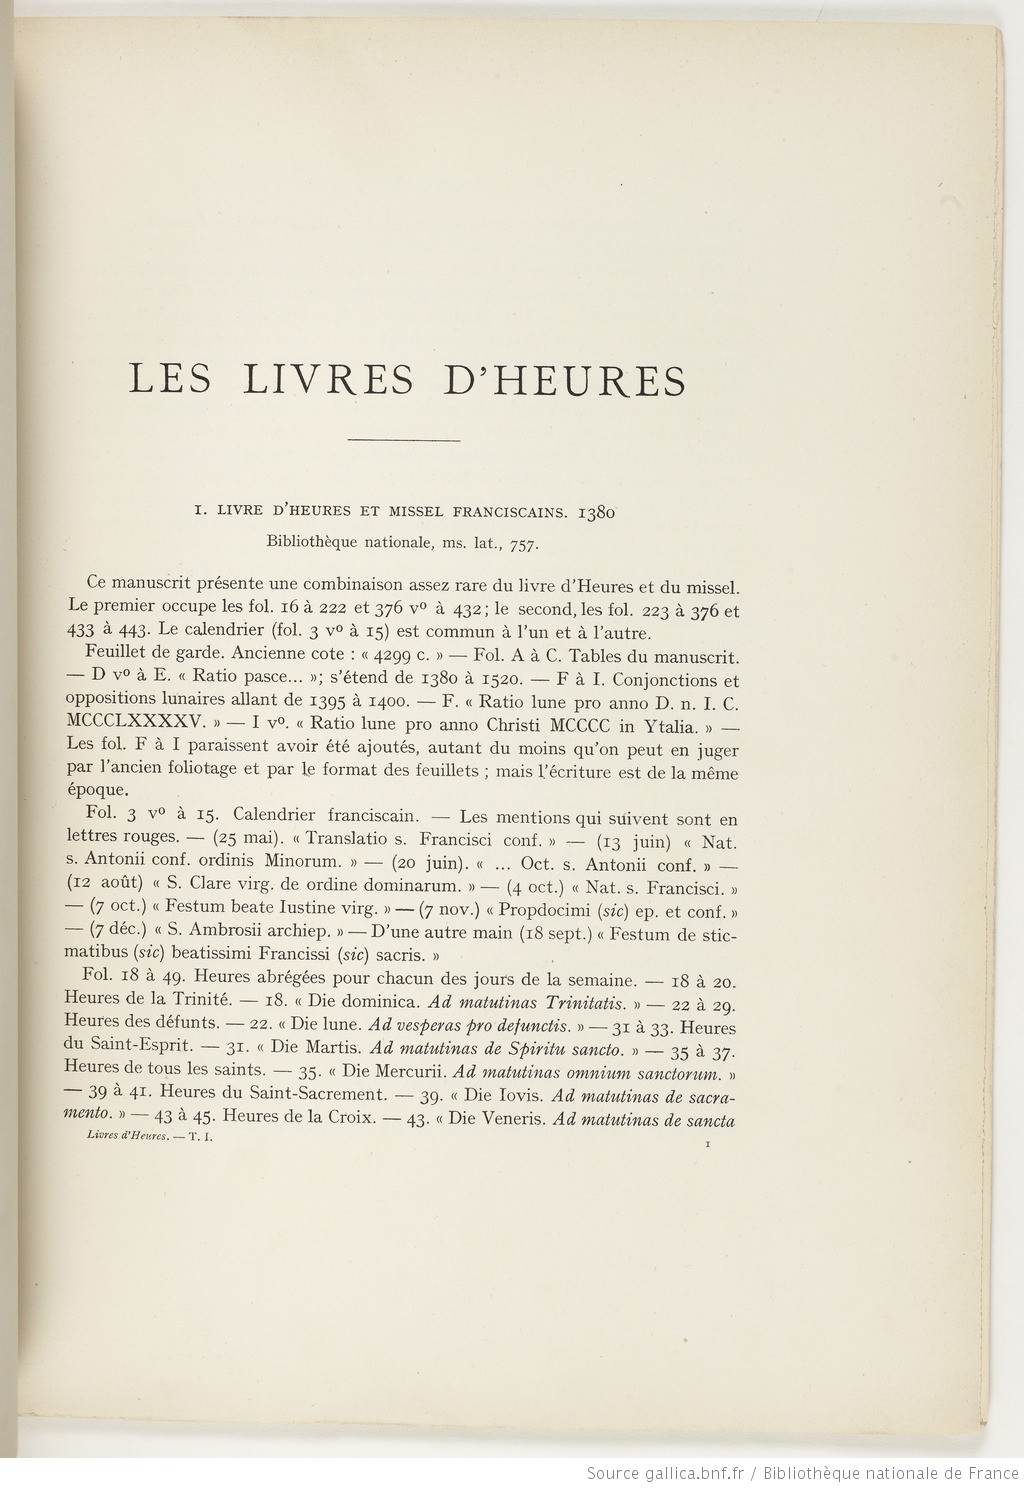
\includegraphics[width=15cm]{img/Notices_Leroquais/Notice1/Papier/noticepapier_1_1.jpeg}
    \caption{Notice 1 numérisée, première page. Cf. \cite[p. 1]{Leroquais_notices}}
    \end{figure}
    \clearpage
    
    \begin{figure}[!h]
    \centering
    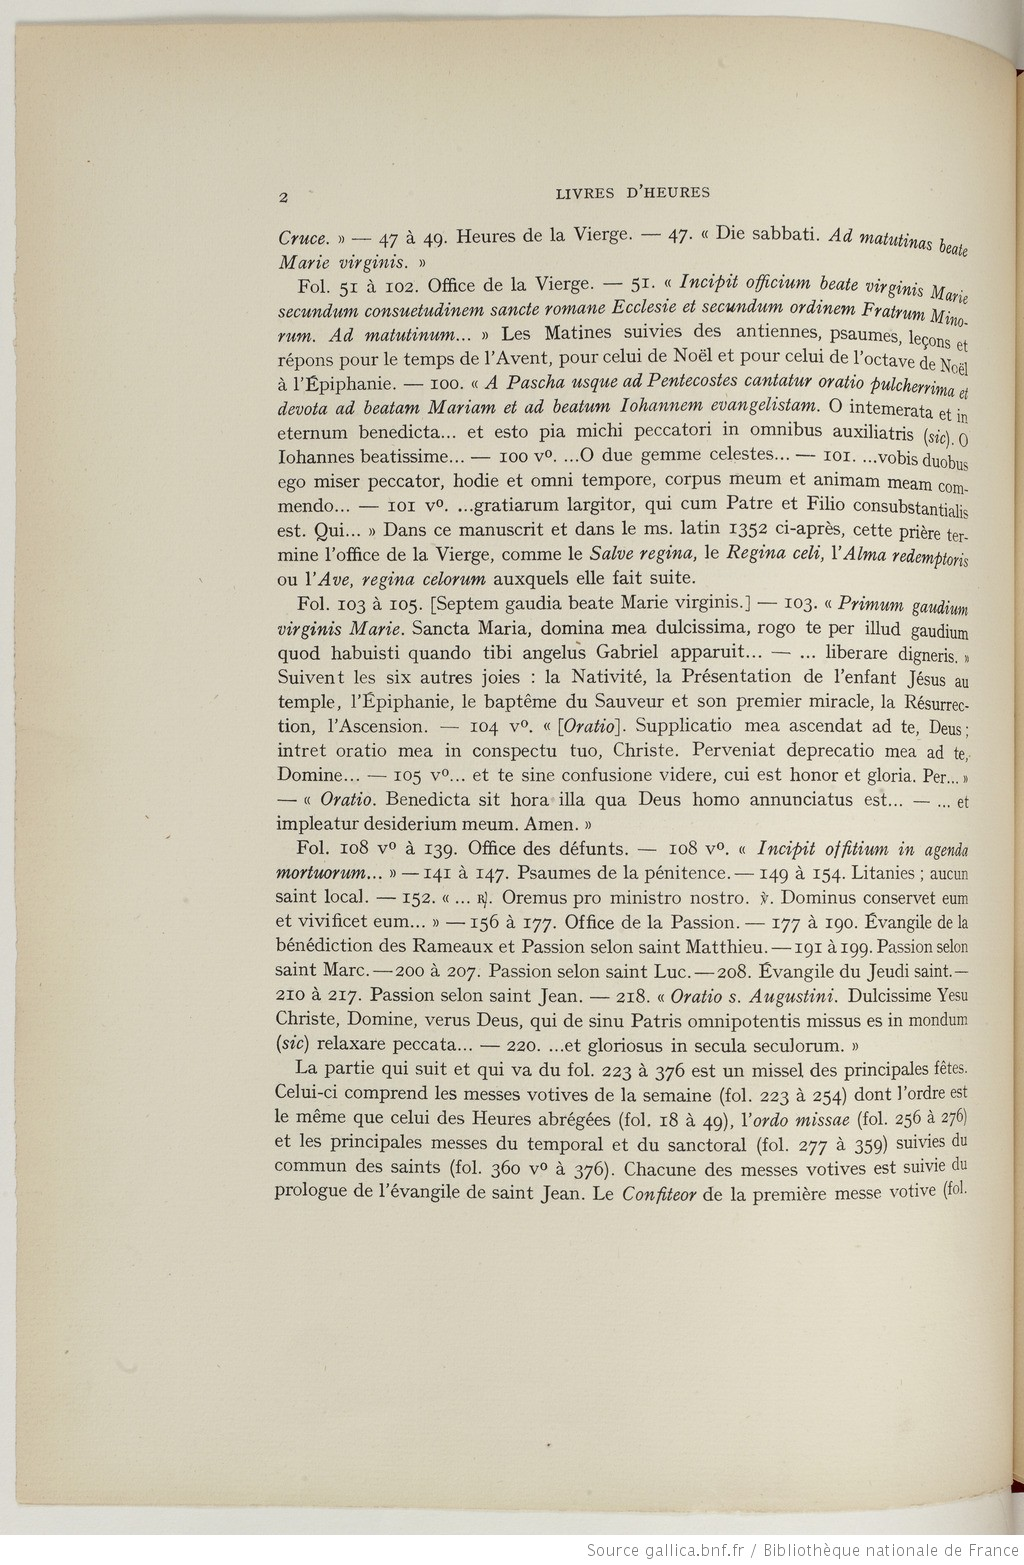
\includegraphics[width=15cm]{img/Notices_Leroquais/Notice1/Papier/noticepapier_1_2.jpeg}
    \caption{Notice 1 numérisée, deuxième page. Cf. \cite[p. 2]{Leroquais_notices}}
    \end{figure}
    \clearpage
    
    \begin{figure}[!h]
    \centering
    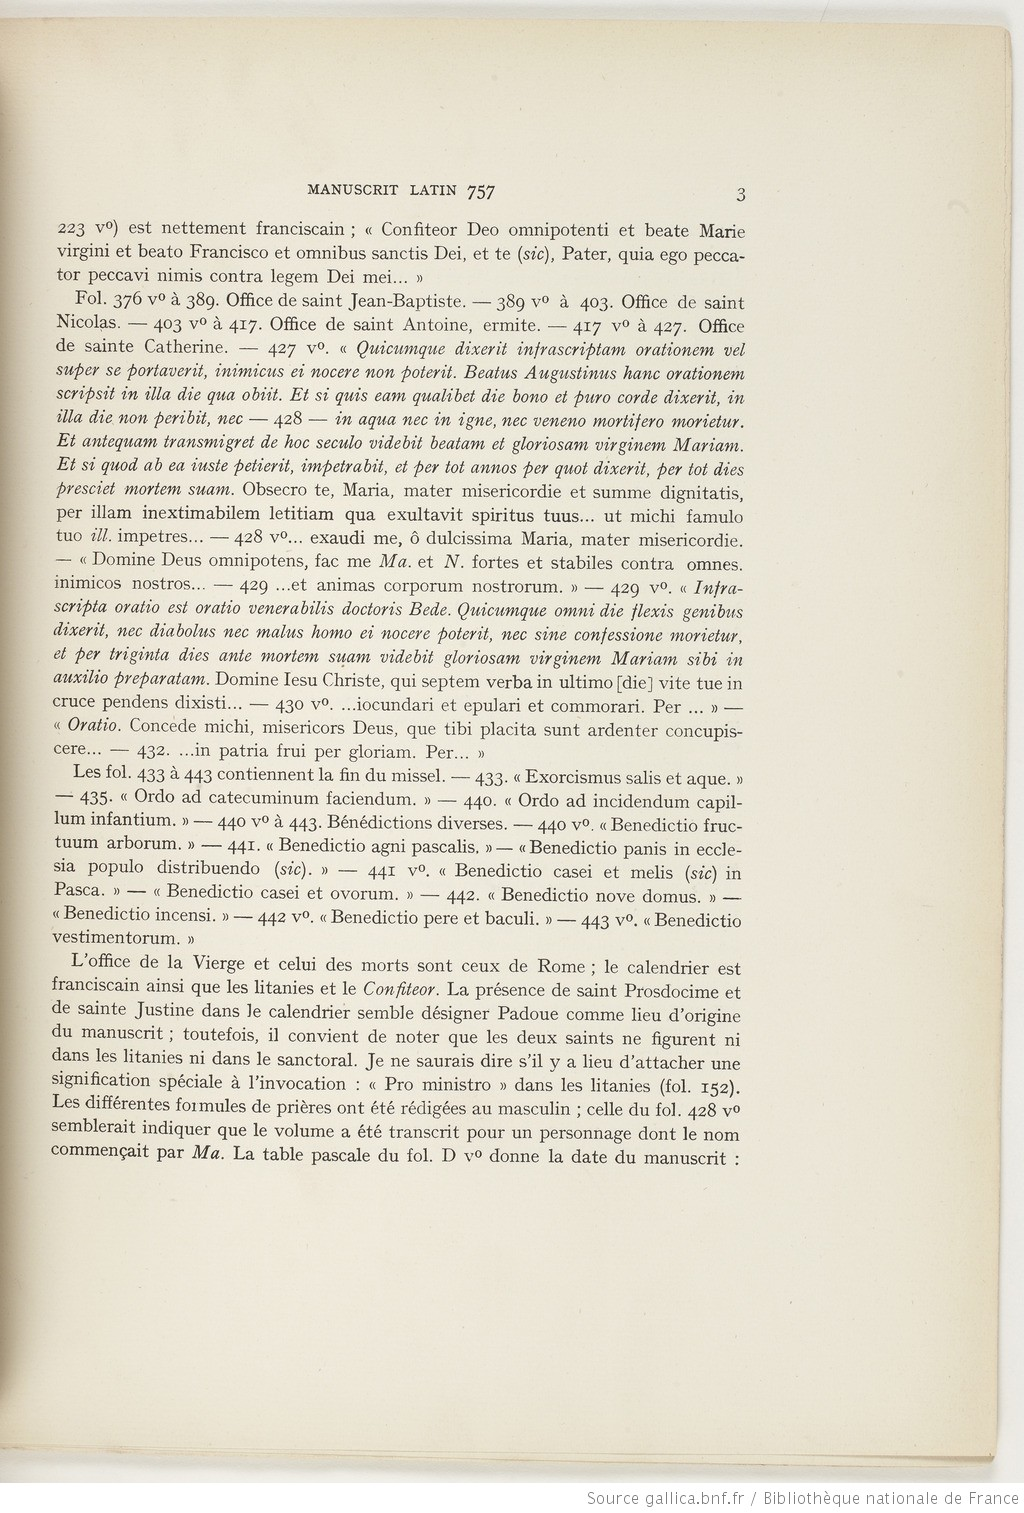
\includegraphics[width=15cm]{img/Notices_Leroquais/Notice1/Papier/notice_papier_1_3.jpeg}
    \caption{Notice 1 numérisée, troisième page. Cf. \cite[p. 3]{Leroquais_notices}}
    \end{figure}
    \clearpage
    
    \begin{figure}[!h]
    \centering
    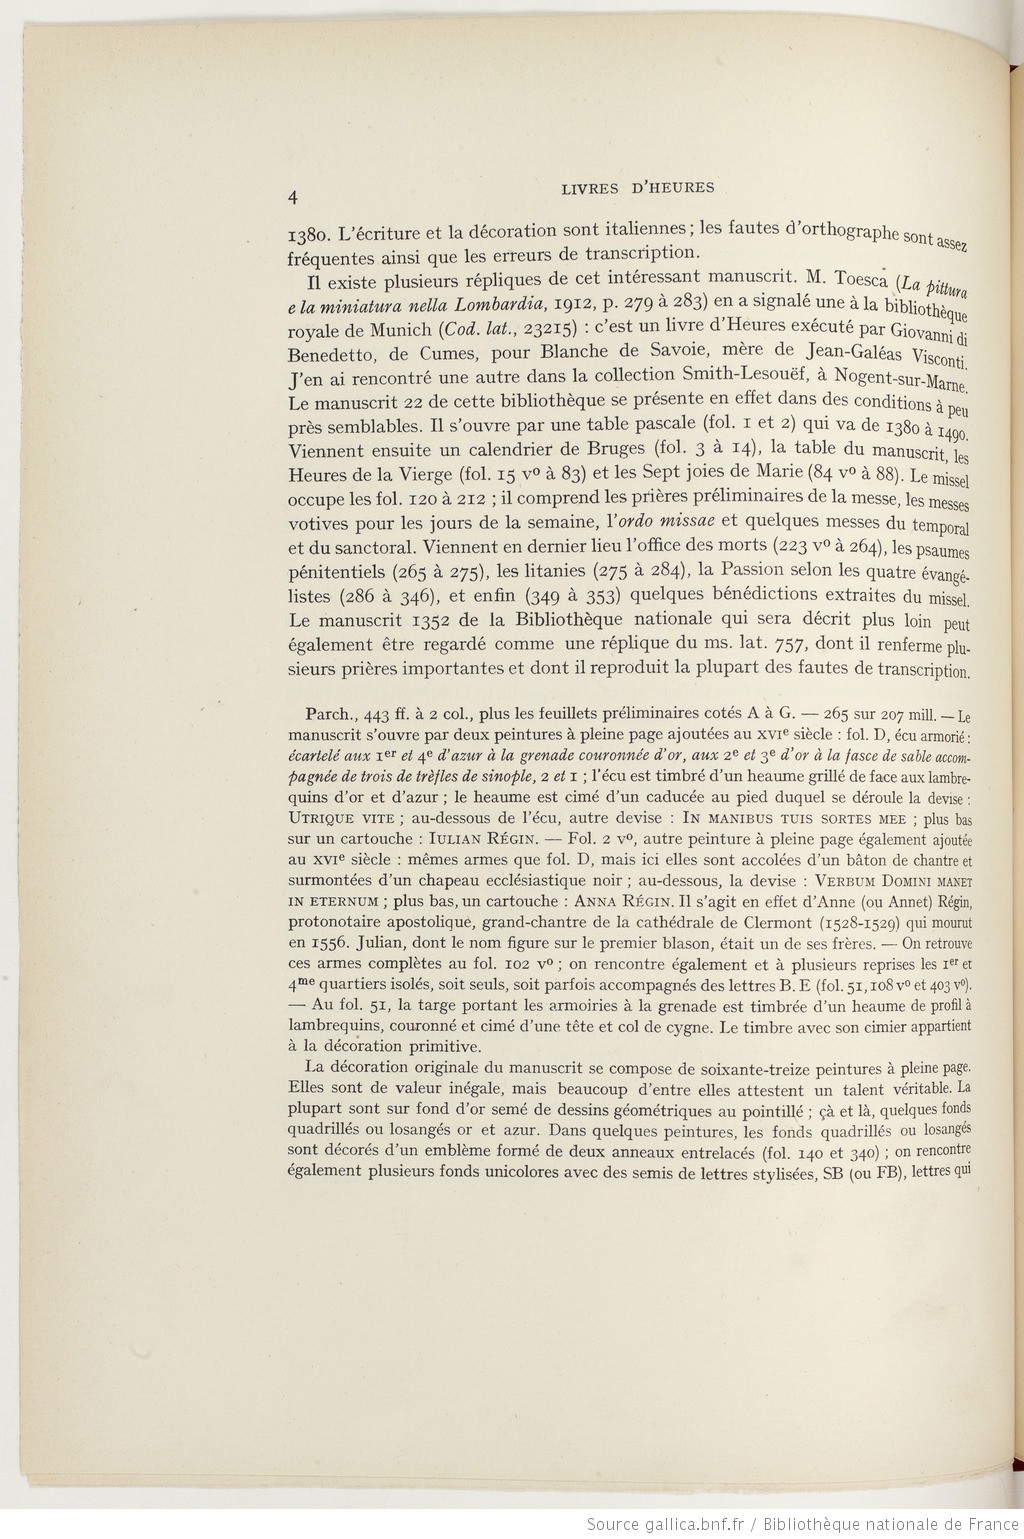
\includegraphics[width=15cm]{img/Notices_Leroquais/Notice1/Papier/notice_papier_1_4.jpeg}
    \caption{Notice 1 numérisée, quatrième page. Cf. \cite[p. 4]{Leroquais_notices}}
    \end{figure}
    \clearpage
    
    \begin{figure}[!h]
    \centering
    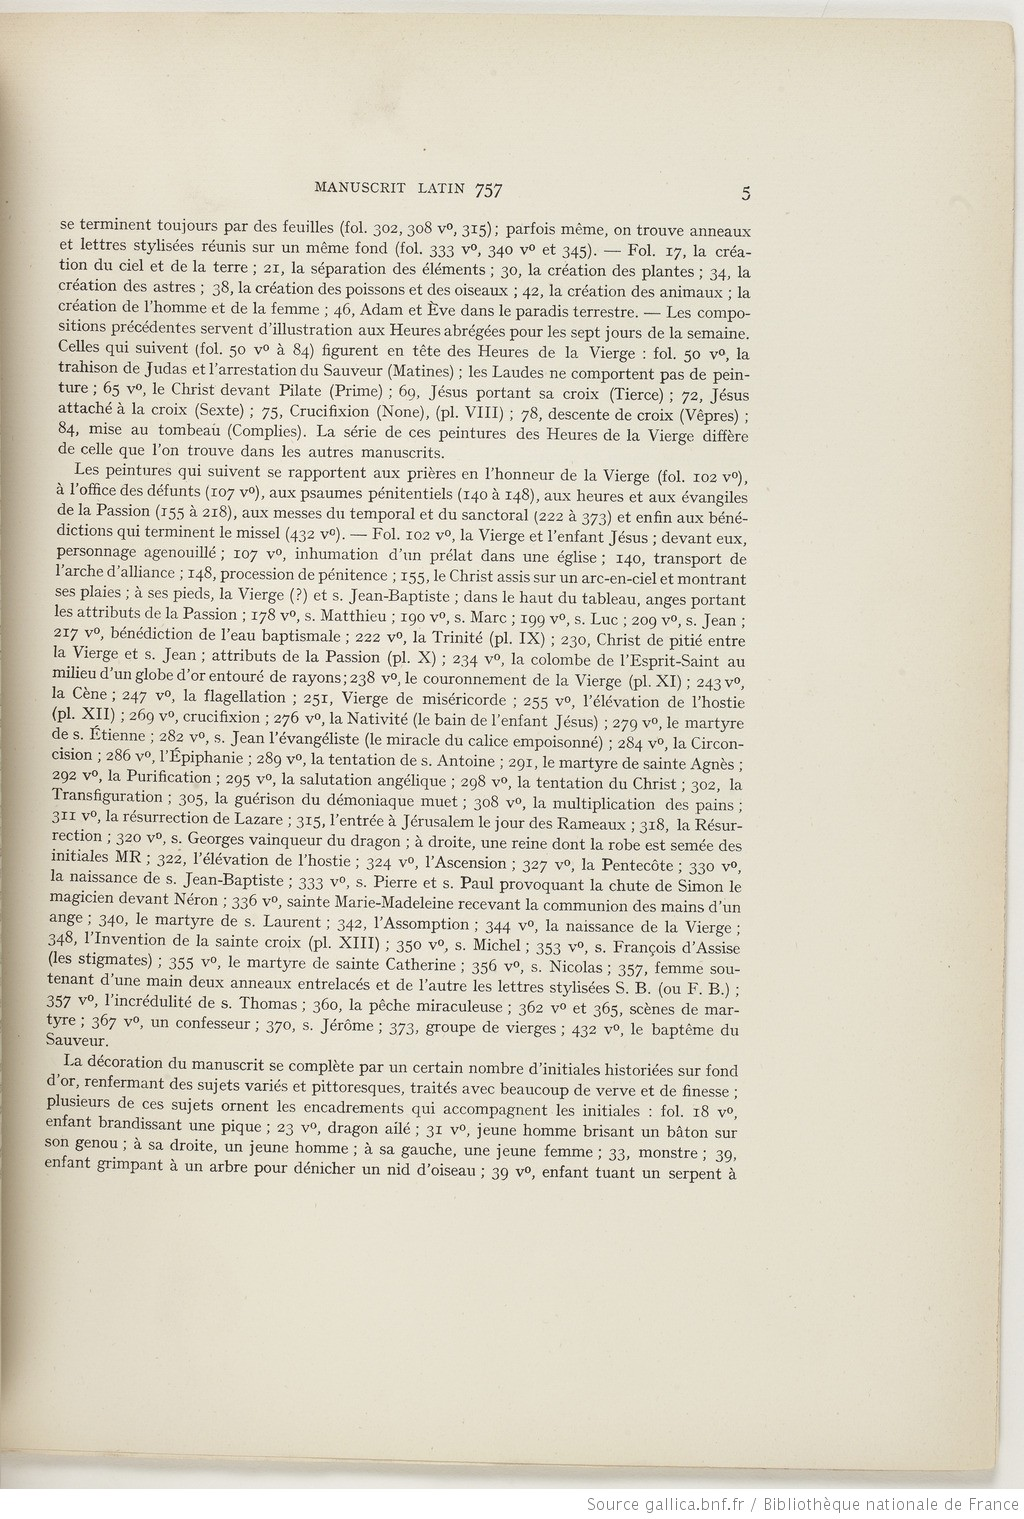
\includegraphics[width=15cm]{img/Notices_Leroquais/Notice1/Papier/notice_papier_1_5.jpeg}
    \caption{Notice 1 numérisée, cinquième page. Cf. \cite[p. 5]{Leroquais_notices}}
    \end{figure}
    \clearpage
    
    \begin{figure}[!h]
    \centering
    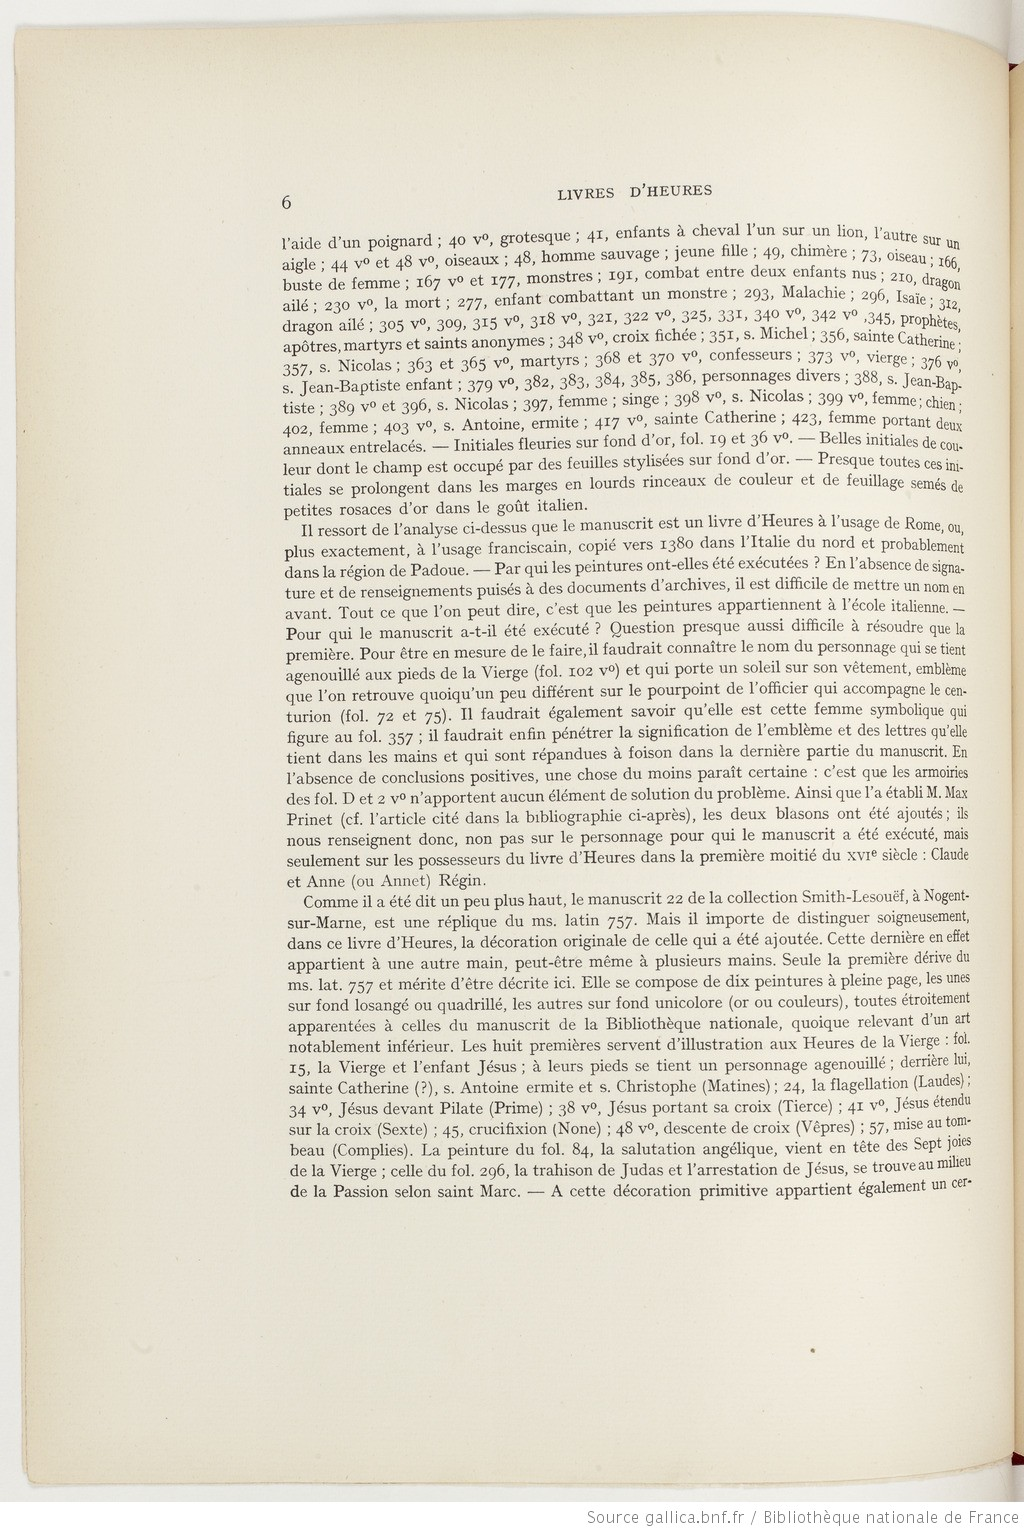
\includegraphics[width=15cm]{img/Notices_Leroquais/Notice1/Papier/notice_papier_1_6.jpeg}
    \caption{Notice 1 numérisée, sixième page. Cf. \cite[p. 6]{Leroquais_notices}}
    \end{figure}
    \clearpage
    
    \begin{figure}[!h]
    \centering
    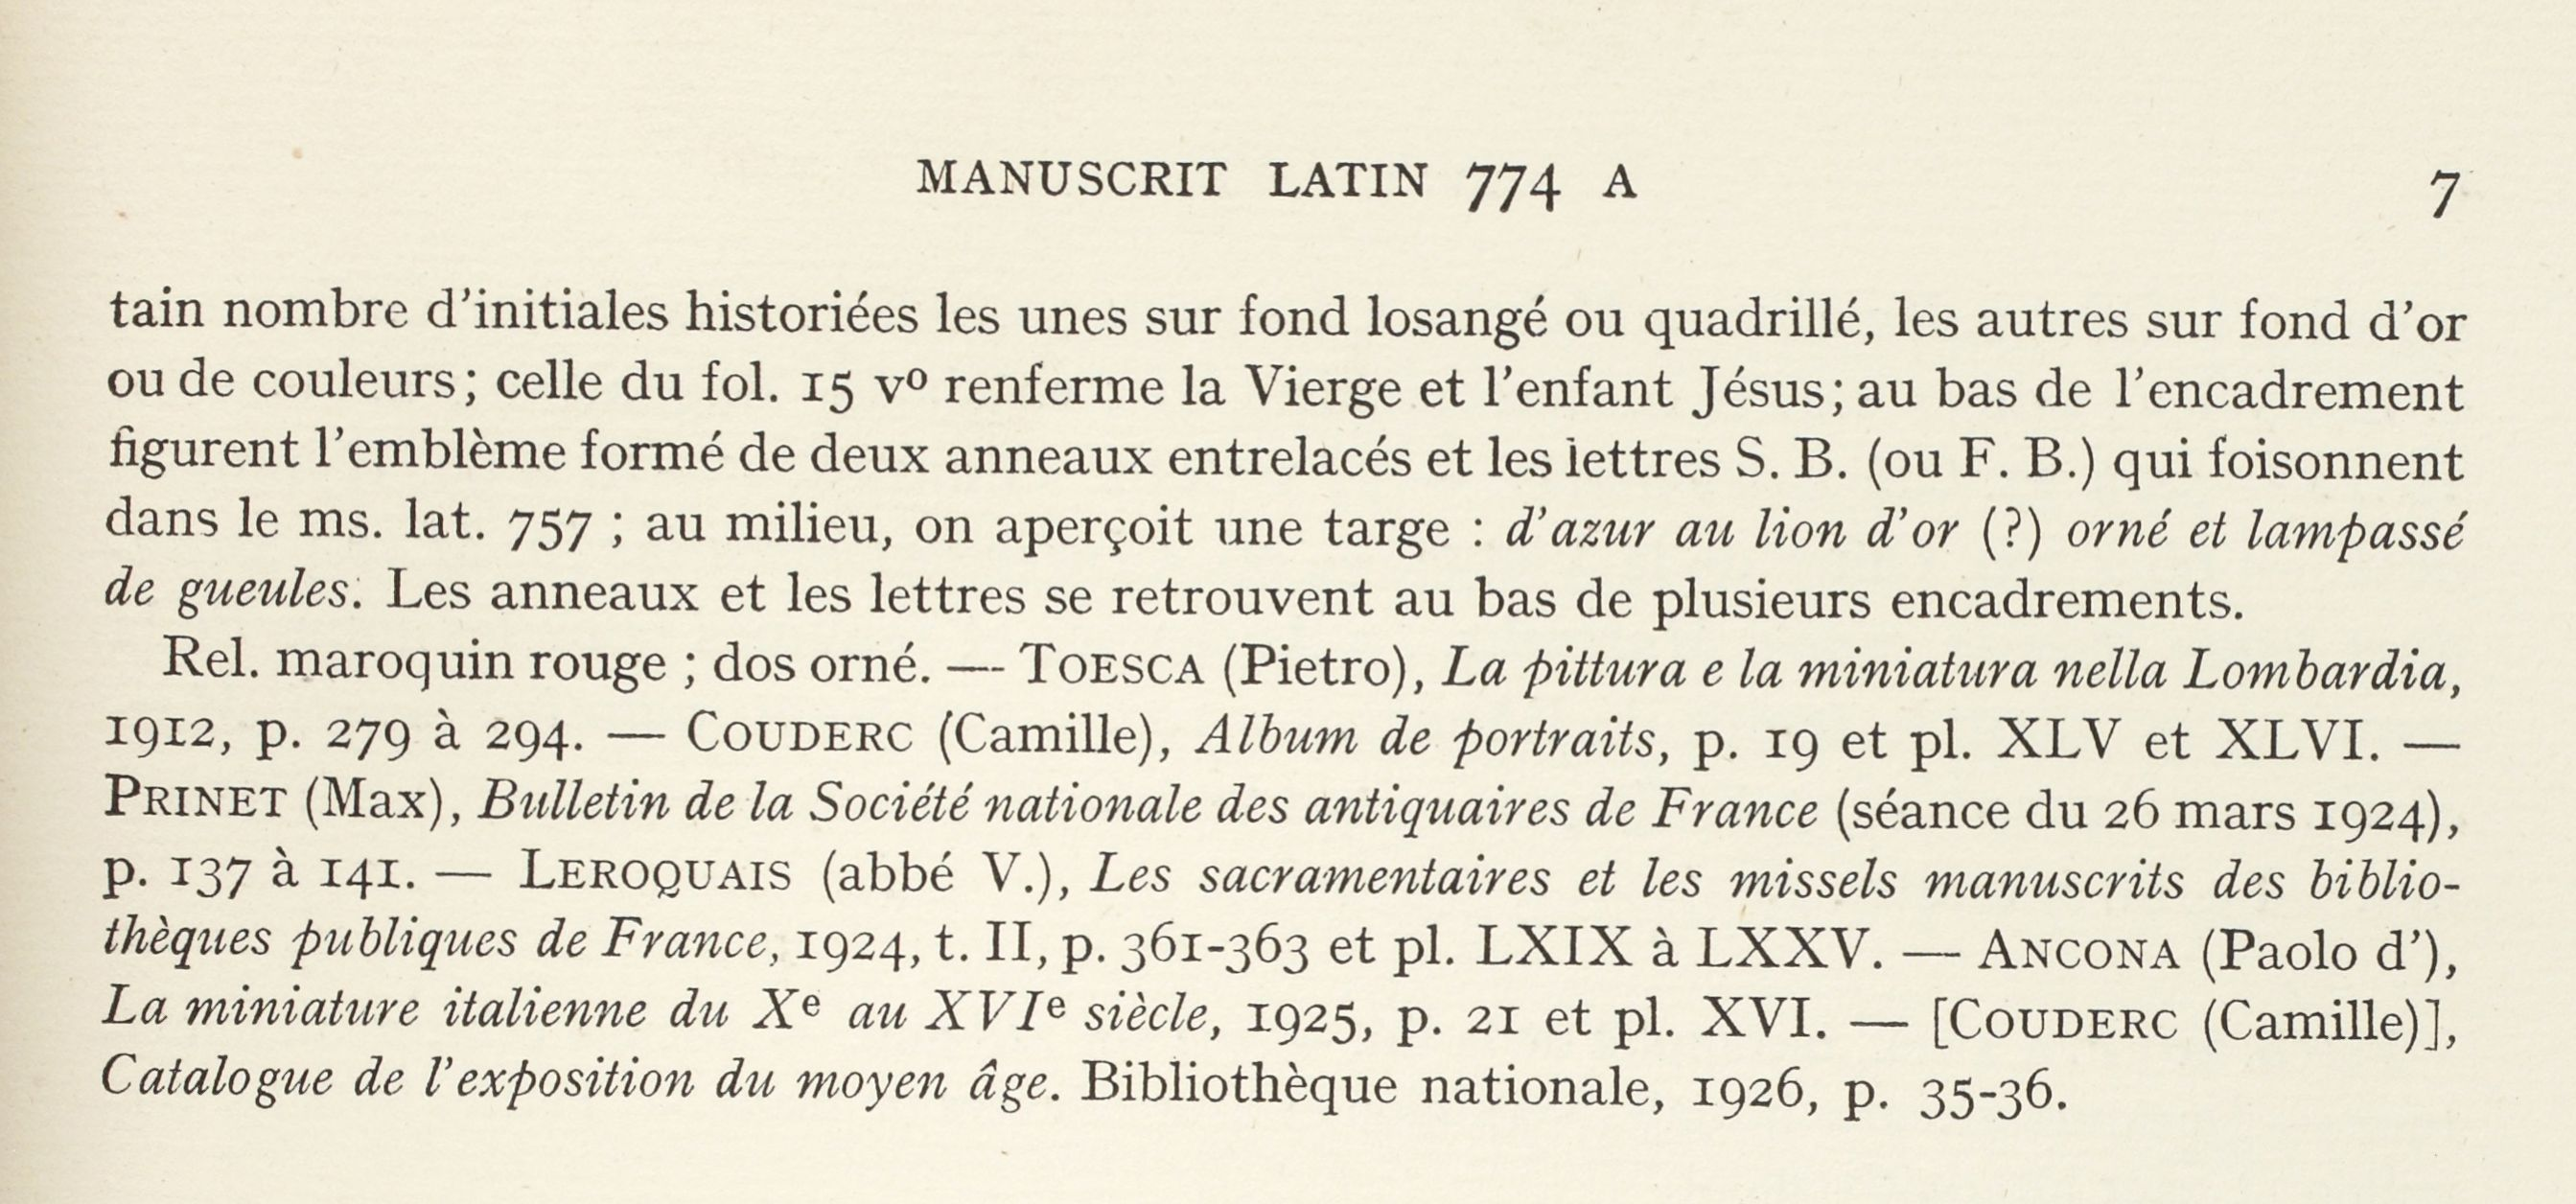
\includegraphics[width=15cm]{img/Notices_Leroquais/Notice1/Papier/notice_papier_1_7.jpg}
    \caption{Notice 1 numérisée, septième page. Cf. \cite[p. 7]{Leroquais_notices}}
    \end{figure}
    \clearpage
    
    %\subsubsection{Notice 112}
    
    \begin{figure}[!h]
    \centering
    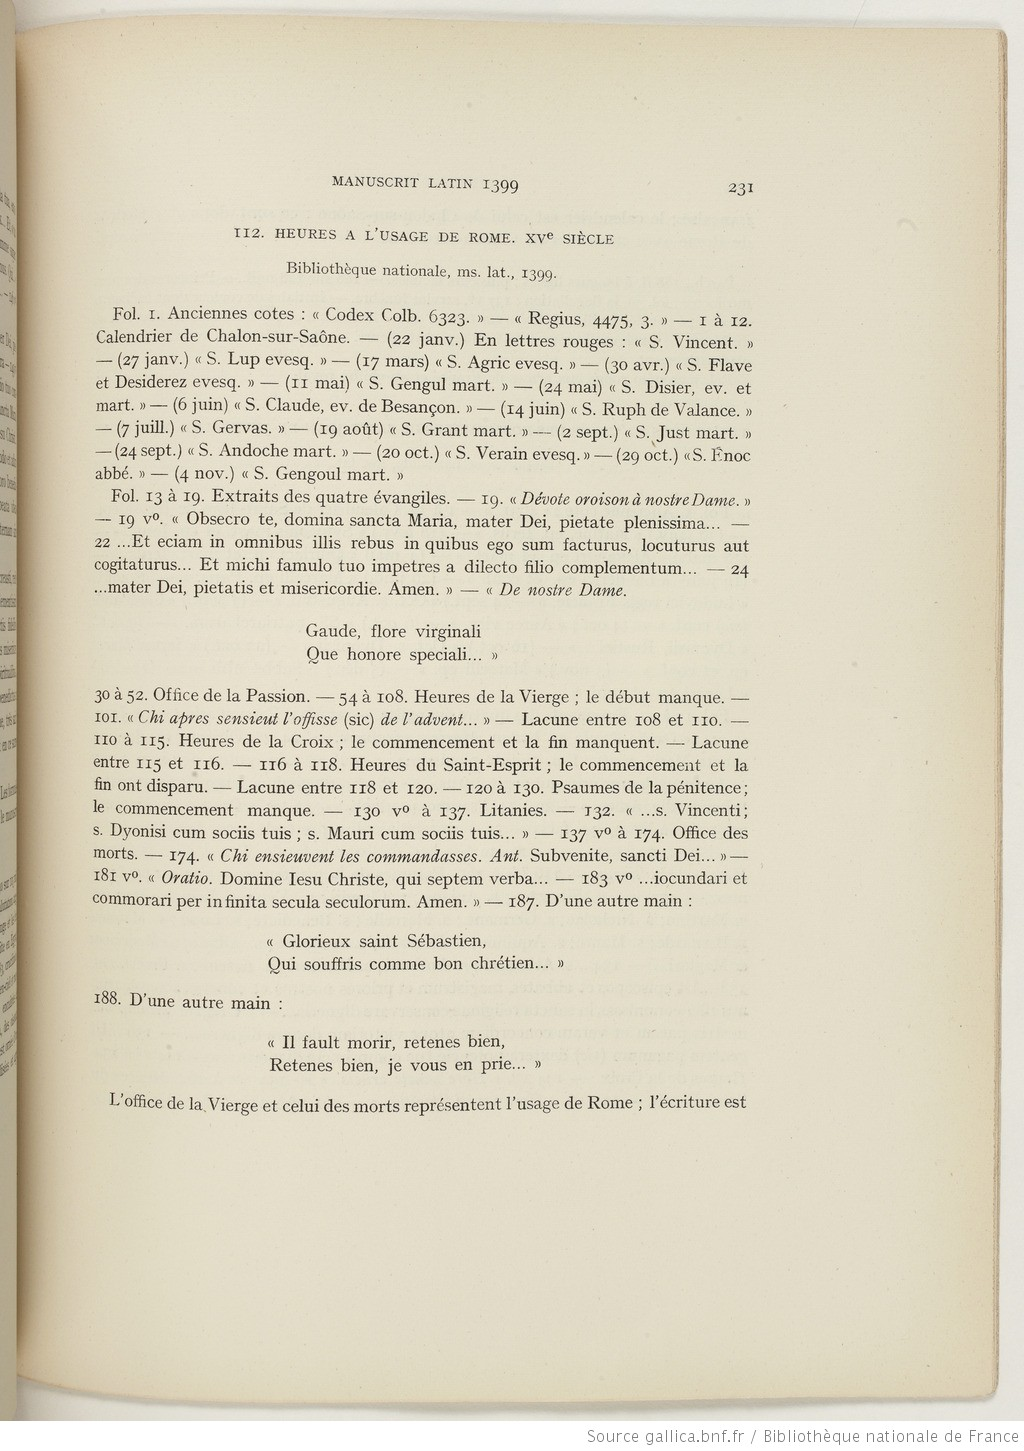
\includegraphics[width=15cm]{img/Notices_Leroquais/Notice112/Papier/notice_papier_112_1.jpeg}
    \caption{Notice 112 numérisée, première page. Cf. \cite[p. 231]{Leroquais_notices}}
    \end{figure}
    \clearpage
    
    \begin{figure}[!h]
    \centering
    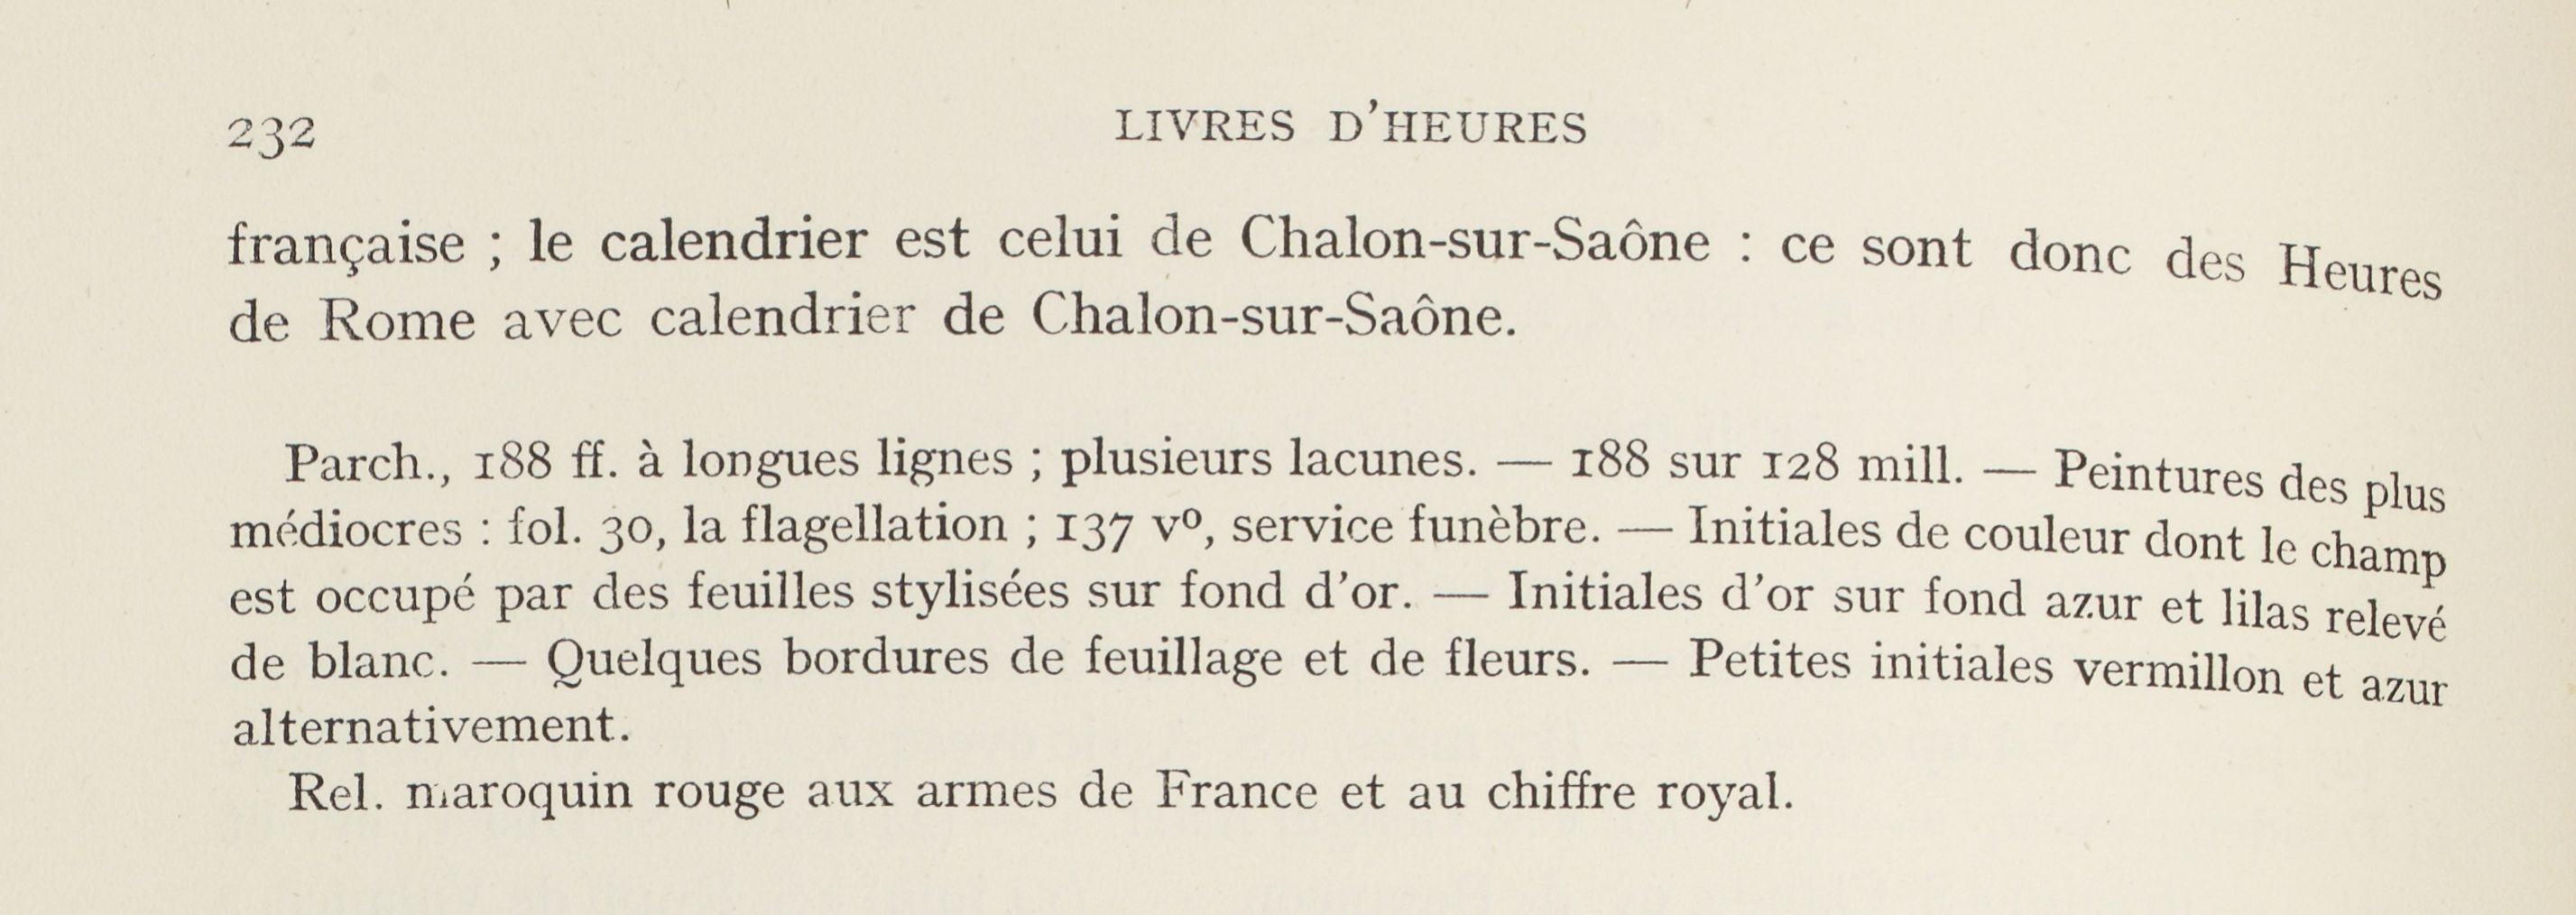
\includegraphics[width=15cm]{img/Notices_Leroquais/Notice112/Papier/notice_papier-112_2.jpg}
    \caption{Notice 112 numérisée, deuxième page. Cf. \cite[p. 232]{Leroquais_notices}}
    \end{figure}
    \clearpage
    
    %\subsubsection{Notice 313}
    
    \begin{figure}[!h]
    \centering
    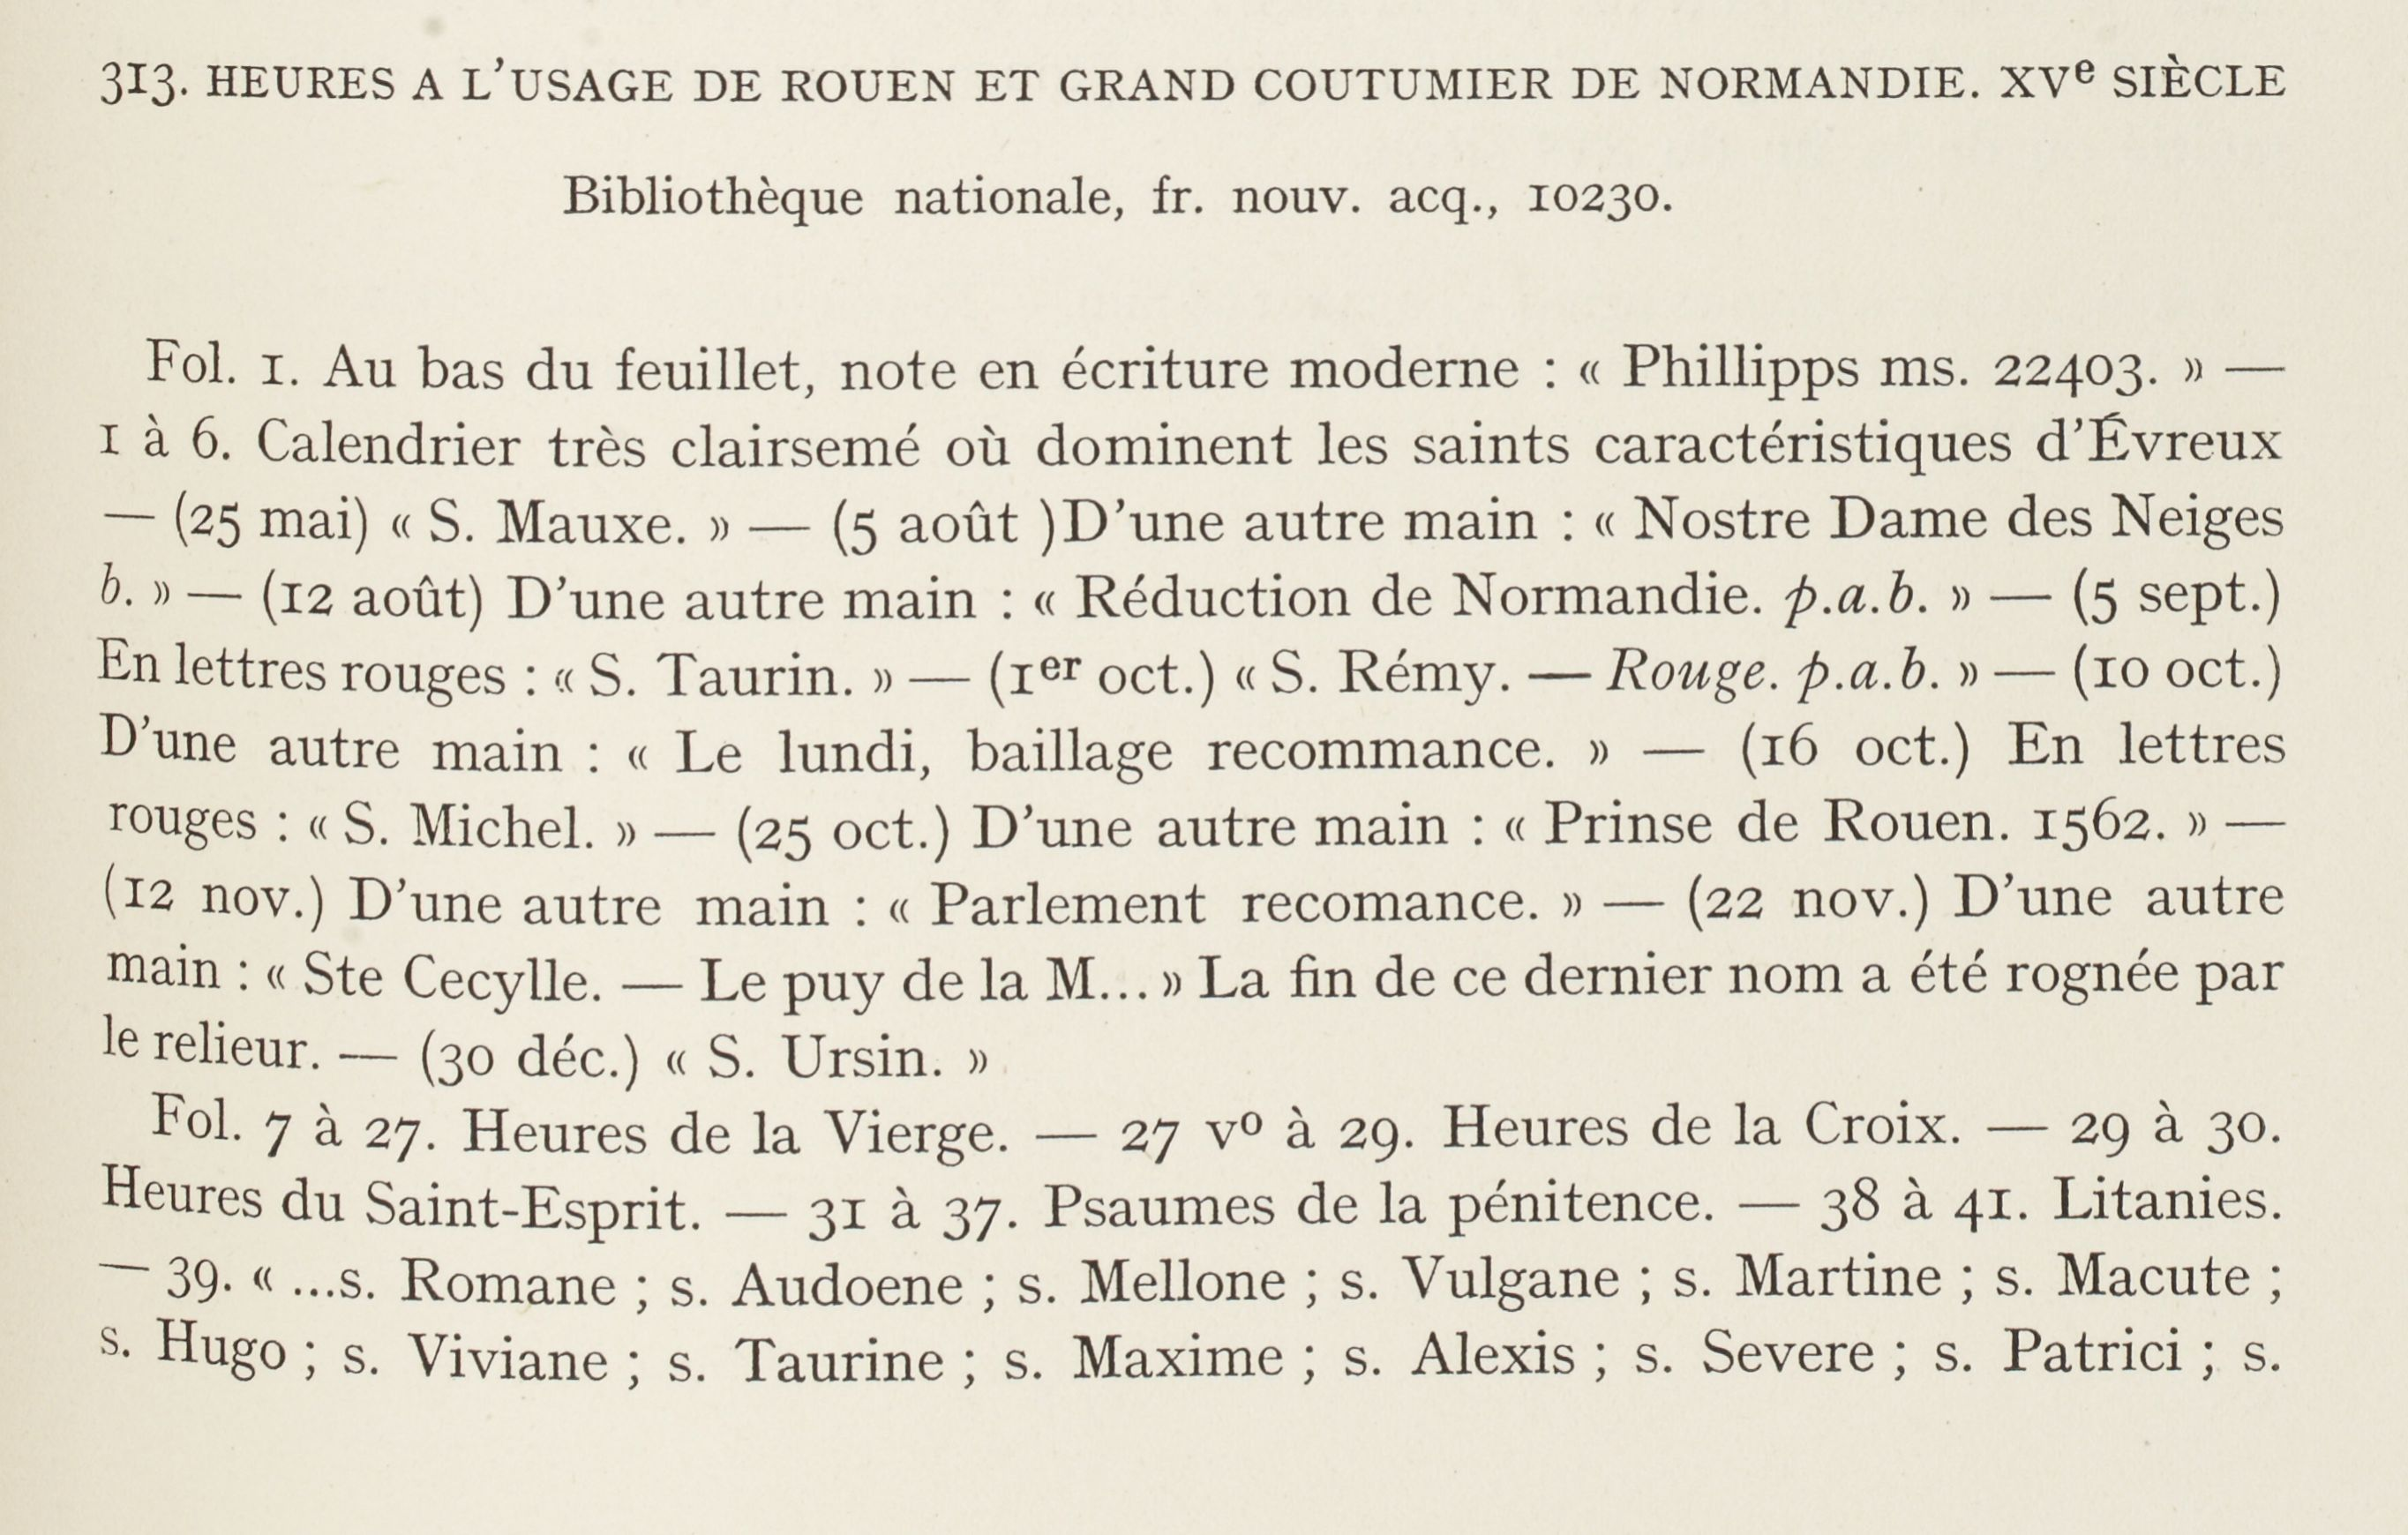
\includegraphics[width=15cm]{img/Notices_Leroquais/Notice313/Papier/noticepapier_313_1.jpg}
    \caption{Notice 313 numérisée, première page. Cf. \cite[p. 304]{Leroquais_notices}}
    \end{figure}
    \clearpage
    
    \begin{figure}[!h]
    \centering
    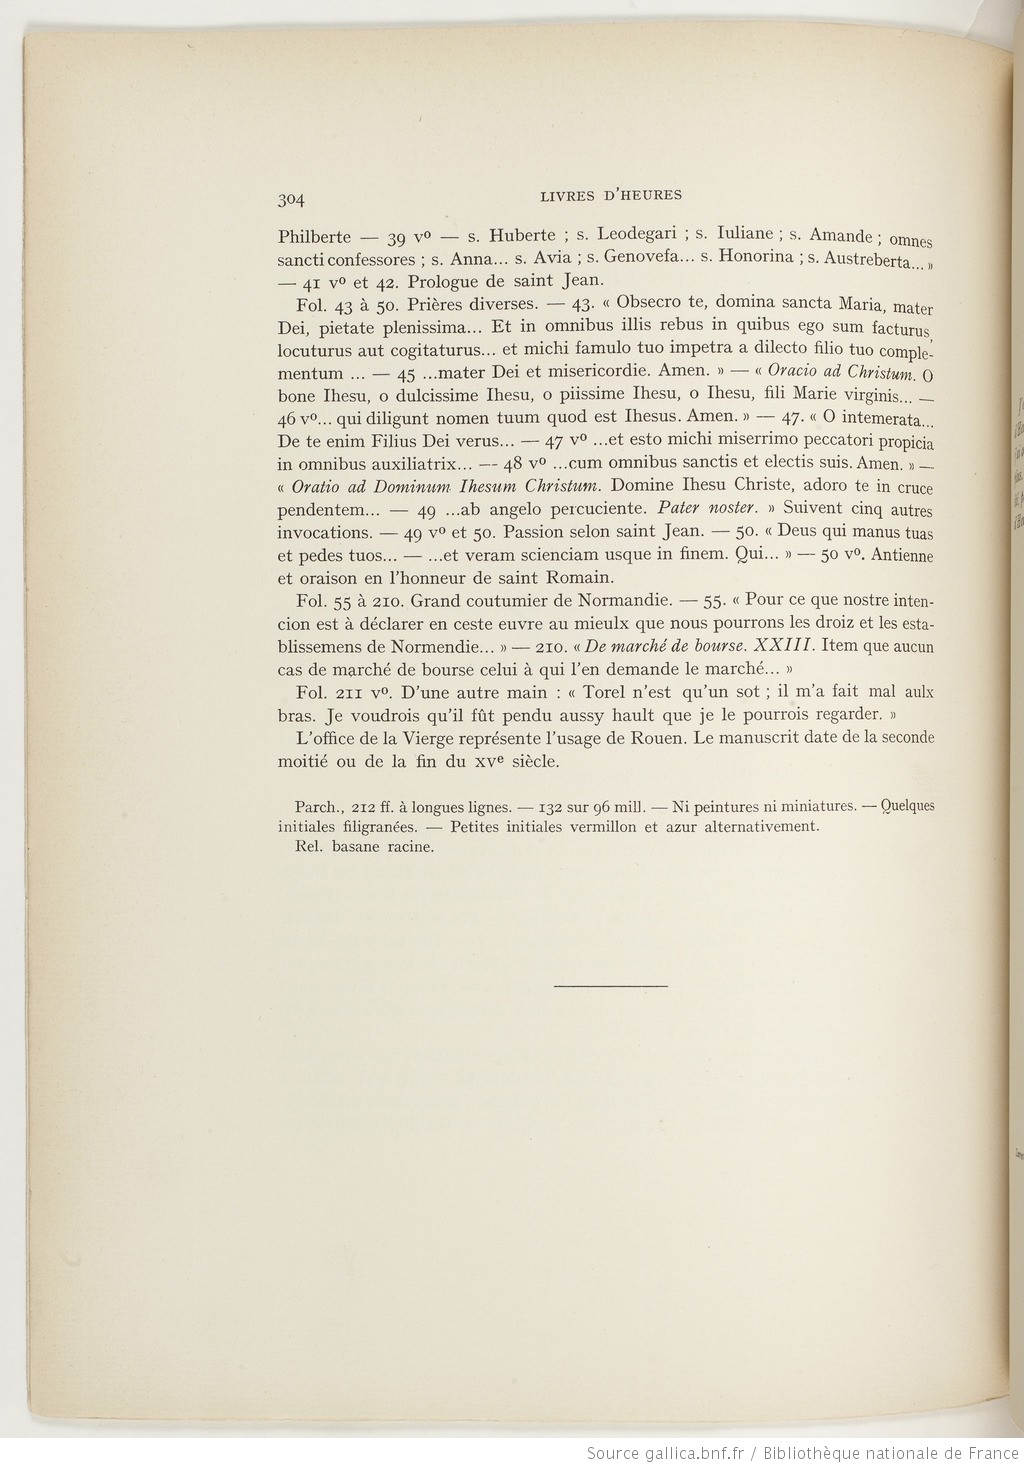
\includegraphics[width=15cm]{img/Notices_Leroquais/Notice313/Papier/notice_papier_313_2.jpeg}
    \caption{Notice 313 numérisée, deuxième page. Cf. \cite[p. 305]{Leroquais_notices}}
    \end{figure}
    \clearpage
	
	\subsection{Notices océrisées}
	
	%\subsubsection{Notice 1}
	
	\begin{figure}[!h]
    \centering
    \includegraphics[width=15cm]{img/Notices_Leroquais/Notice1/OCR/Notice_OCR_1_1.png}
    \caption{Notice 1 océrisée, première page}
    \end{figure}
    \clearpage
    
    \begin{figure}[!h]
    \centering
    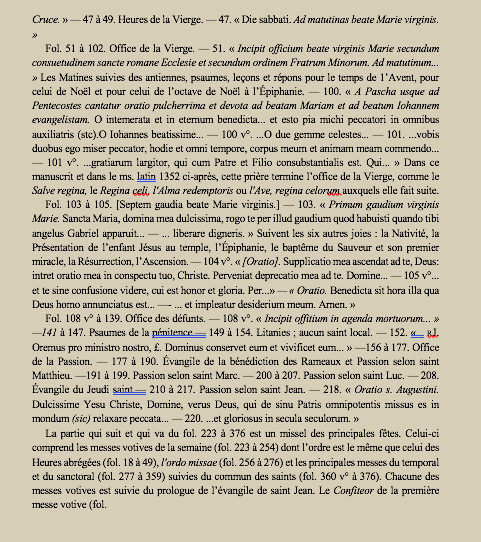
\includegraphics[width=15cm]{img/Notices_Leroquais/Notice1/OCR/notice_OCR_1_2.png}
    \caption{Notice 1 océrisée, deuxième page}
    \end{figure}
    \clearpage
    
    \begin{figure}[!h]
    \centering
    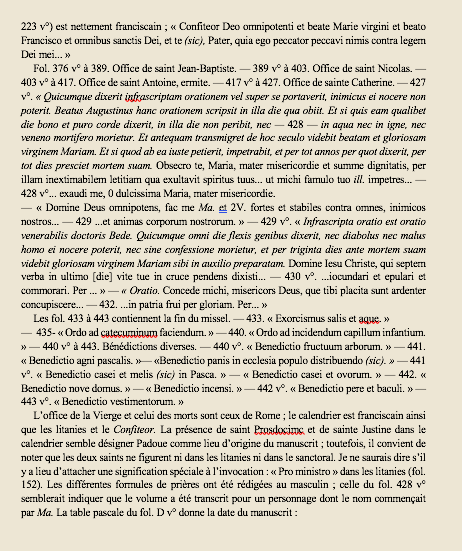
\includegraphics[width=15cm]{img/Notices_Leroquais/Notice1/OCR/notice_OCR_1_3.png}
    \caption{Notice 1 océrisée, troisième page}
    \end{figure}
    \clearpage
    
    \begin{figure}[!h]
    \centering
    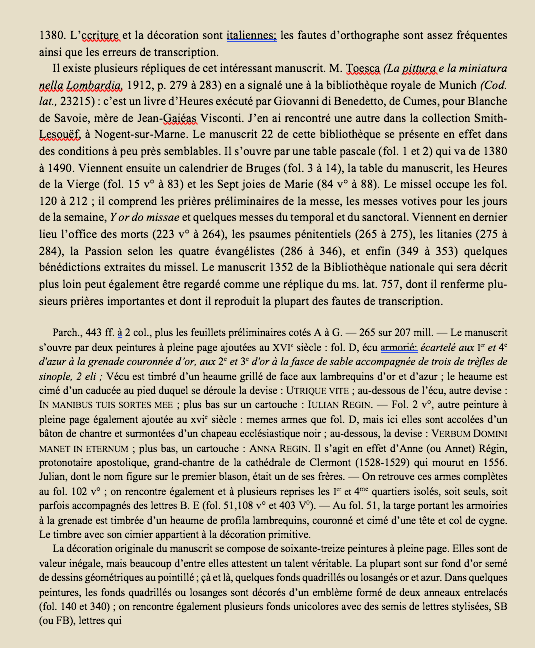
\includegraphics[width=15cm]{img/Notices_Leroquais/Notice1/OCR/notice_OCR_1_4.png}
    \caption{Notice 1 océrisée, quatrième page}
    \end{figure}
    \clearpage
    
    \begin{figure}[!h]
    \centering
    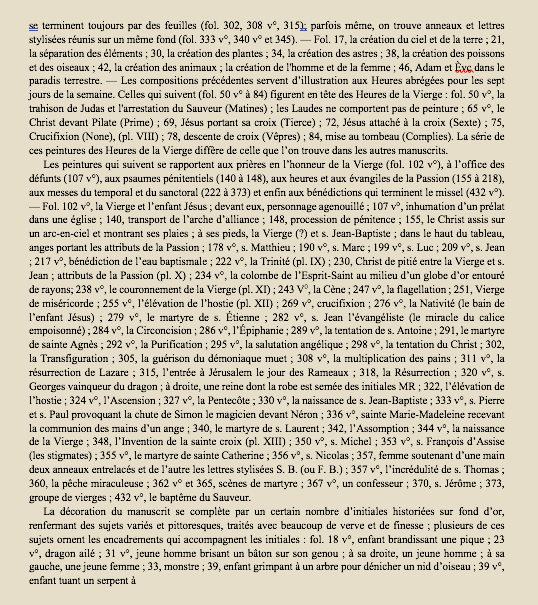
\includegraphics[width=15cm]{img/Notices_Leroquais/Notice1/OCR/notice_OCR_1_5.png}
    \caption{Notice 1 océrisée, cinquième page}
    \end{figure}
    \clearpage
    
    \begin{figure}[!h]
    \centering
    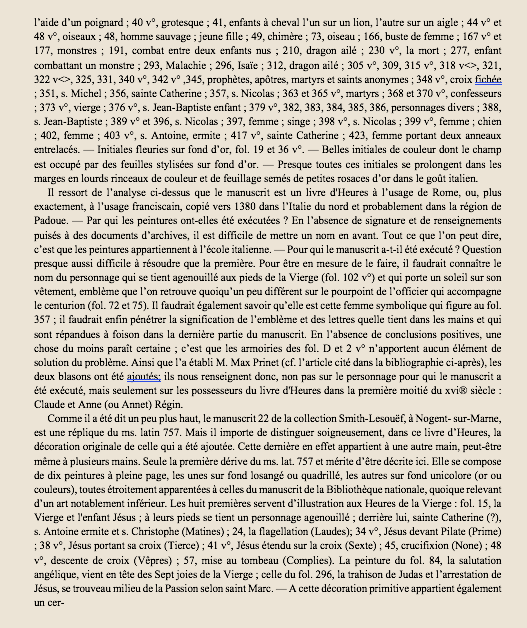
\includegraphics[width=15cm]{img/Notices_Leroquais/Notice1/OCR/notice_OCR_1_6.png}
    \caption{Notice 1 océrisée, sixième page}
    \end{figure}
    \clearpage
    
    \begin{figure}[!h]
    \centering
    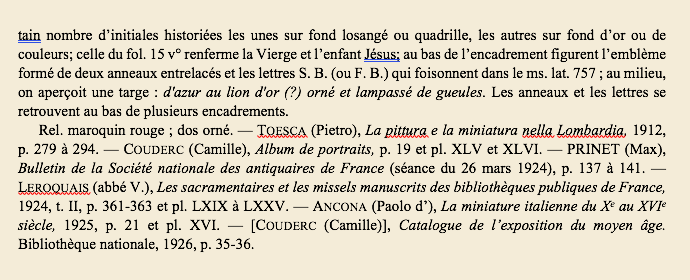
\includegraphics[width=15cm]{img/Notices_Leroquais/Notice1/OCR/notice_OCR_1_7.jpeg}
    \caption{Notice 1 océrisée, septième page}
    \end{figure}
    \clearpage
    
    %\subsubsection{Notice 112}
    
    \begin{figure}[!h]
    \centering
    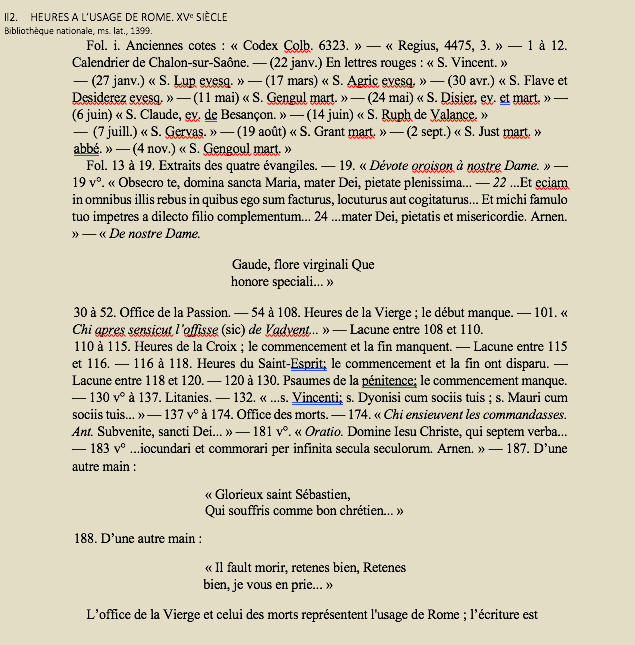
\includegraphics[width=15cm]{img/Notices_Leroquais/Notice112/OCR/NoticeOCR_112_1.png}
    \caption{Notice 112 océrisée, première page}
    \end{figure}
    \clearpage
    
    \begin{figure}[!h]
    \centering
    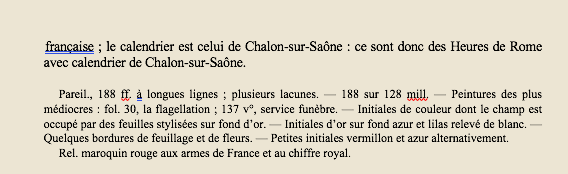
\includegraphics[width=15cm]{img/Notices_Leroquais/Notice112/OCR/noticeOCR_112_2.png}
    \caption{Notice 112 océrisée, deuxième page}
    \end{figure}
    \clearpage
    
    %\subsubsection{Notice 313}
    
	\begin{figure}[!h]
    \centering
    \includegraphics[width=15cm]{img/Notices_Leroquais/Notice313/OCR/noticeOCR_313_1.png}
    \caption{Notice 313 océrisée, première page}
    \end{figure}
    \clearpage
    
    \begin{figure}[!h]
    \centering
    \includegraphics[width=15cm]{img/Notices_Leroquais/Notice313/OCR/notice_OCR_313_2.png}
    \caption{Notice 313 océrisée, deuxième page}
    \end{figure}
    \clearpage
	
	\subsection{Analyses du document à encoder}
	
	La phase d'observation des documents à encoder le plus automatiquement possible s'est concrétisée par la formalisation d'arbres de décision, censés refléter d'un part la structure des notices et d'autre part leurs irrégularités. Face à ces cas concrets s'offre un ensemble de choix et de décisions à prendre selon le document de sortie \textit{in fine} souhaité. L'arbre de décision a pour intérêt de souligner les grandes étapes qui doivent apparaître dans le code de transformation. 
	
	\subsubsection{\label{arbre_decision_1}Arbre de décision : première version}
	
	La version ici proposée a pour principal atout de mettre en valeur la structure finale souhaitée en partant du document d'origine. Il permet donc de visualiser, selon les balises TEI, où se trouve les informations à encoder dans le document source, et donc d'avoir conscience des informations qui se trouvent à divers endroits du document d'origine mais qui sont ensuite regroupées sous une même balise. Si cette situation reste relativement rare, l'information relevant de la balise \textless summary\textgreater~illustre ce cas. Désignant ce qui concerne le contenu général du manuscrit, l'information se situe systématiquement dans le titre de la notice en majuscule, mais aussi parfois dans un premier paragraphe. 
	Toutefois, cette version a pour défaut de ne pas assez représenter la structure des notices rédigées par Leroquais. 
	
	\includepdf[pages = {1-2}]{img/Notices_Leroquais/ArbreDecisionVersion1.pdf}
	
	\subsubsection{\label{arbre_decision_2}Arbre de décision : deuxième version}
	
	Contrairement à la première, cette deuxième version se veut plus proche du document d'origine à encoder, tout en soulignant les solutions, difficultés et interrogations qui ont émergées autour de la possibilité d'une automatisation de l'encodage.
	
	\includepdf[pages = {1-6}]{img/Notices_Leroquais/ArbreDecisionVersion2.pdf}
	
	\subsection{Définition du document cible}
	
	\subsubsection{\label{personnalisation_ODD}Personnalisation du fichier ODD relatif au msDesc}
	
	\begin{minted}{XML}
<!--Checking module msdescription-->
            <classRef key="att.msClass"/>
            <classRef key="model.physDescPart"/>
            <moduleRef key="msdescription"
                       include="msDesc catchwords dimensions dim height 
                       width locus material origDate origPlace 
                       signatures watermark msIdentifier repository 
                       altIdentifier colophon explicit finalRubric 
                       incipit msContents msItem rubric summary 
                       physDesc objectDesc supportDesc support 
                       collation foliation condition layoutDesc 
                       layout handDesc scriptDesc musicNotation 
                       decoDesc decoNote bindingDesc binding 
                       history origin provenance additional 
                       adminInfo recordHist source surrogates msPart"/>
            <elementSpec ident="msDesc" mode="change">
               <attList>
                  <attDef ident="corresp" mode="delete"/>
                  <attDef ident="sameAs" mode="delete"/>
                  <attDef ident="ana" mode="delete"/>
                  <attDef ident="facs" mode="delete"/>
                  <attDef ident="cert" mode="delete"/>
                  <attDef ident="resp" mode="delete"/>
                  <attDef ident="source" mode="delete"/>
                  <attDef ident="type" mode="delete"/>
                  <!-- Suppression de l'attribut "status" qui apparaît 
                  systématiquement sur l'élément <msDesc> 
                  avec la valeur "draft". -->
                  <attDef ident="status" mode="delete" />          
               </attList>
            </elementSpec>
            <elementSpec ident="catchwords" mode="change">
               <attList>
                  <attDef ident="corresp" mode="delete"/>
                  <attDef ident="sameAs" mode="delete"/>
                  <attDef ident="ana" mode="delete"/>
                  <attDef ident="facs" mode="delete"/>
                  <attDef ident="cert" mode="delete"/>
                  <attDef ident="resp" mode="delete"/>
                  <attDef ident="source" mode="delete"/>
               </attList>
            </elementSpec>
            <elementSpec ident="dimensions" mode="change">
               <!-- Définition d'une séquence d'éléments
               à l'intérieur de l'élément "dimensions". -->
               <content>
                  <sequence>
                     <elementRef key="height" minOccurs="1" maxOccurs="1"/>
                     <elementRef key="width" minOccurs="1" maxOccurs="1"/>
                     <elementRef key="dim" minOccurs="0" maxOccurs="1"/>
                  </sequence>
               </content>
               <attList>
                  <!-- Ajout de l'attribut "type" avec les valeurs 
                  suggérées "justification" et "leaf". -->
                  <attDef ident="type" mode="change">
                     <valList mode="add">
                        <valItem ident="justification"/>
                        <valItem ident="leaf"/>
                     </valList>
                  </attDef>
                  <!-- Ajout de l'attribut "scope" avec la valeur 
                  suggérée "all". -->
                  <attDef ident="scope" mode="change">
                     <valList mode="add">
                        <valItem ident="all"/>
                     </valList>
                  </attDef>
                  <!-- Ajout de l'attribut "unit" avec la valeur 
                  "mm" pour normaliser l'unité de mesure. -->
                  <attDef ident="unit" mode="change">
                     <valList mode="add">
                        <valItem ident="mm"/>
                     </valList>
                  </attDef>
                  <!-- Ajout de l'attribut "corresp". -->
                  <attDef ident="corresp" mode="change"/>
                  <attDef ident="sameAs" mode="delete"/>
                  <attDef ident="ana" mode="delete"/>
                  <attDef ident="facs" mode="delete"/>
                  <attDef ident="cert" mode="delete"/>
                  <attDef ident="resp" mode="delete"/>
                  <attDef ident="source" mode="delete"/>
                  <attDef ident="quantity" mode="delete"/>
                  <attDef ident="atLeast" mode="delete"/>
                  <attDef ident="atMost" mode="delete"/>
                  <attDef ident="min" mode="delete"/>
                  <attDef ident="max" mode="delete"/>
               </attList>
            </elementSpec>
            <elementSpec ident="dim" mode="change">
               <attList>
                  <attDef ident="corresp" mode="delete"/>
                  <attDef ident="sameAs" mode="delete"/>
                  <attDef ident="ana" mode="delete"/>
                  <attDef ident="facs" mode="delete"/>
                  <attDef ident="cert" mode="delete"/>
                  <attDef ident="resp" mode="delete"/>
                  <attDef ident="source" mode="delete"/>
                  <attDef ident="type" mode="delete"/>
                  <attDef ident="unit" mode="delete"/>
                  <attDef ident="quantity" mode="delete"/>
                  <attDef ident="scope" mode="delete"/>
                  <attDef ident="atLeast" mode="delete"/>
                  <attDef ident="atMost" mode="delete"/>
                  <attDef ident="min" mode="delete"/>
                  <attDef ident="max" mode="delete"/>
               </attList>
            </elementSpec>
            <elementSpec ident="height" mode="change">
               <attList>
                  <attDef ident="sameAs" mode="delete"/>
                  <attDef ident="ana" mode="delete"/>
                  <attDef ident="facs" mode="delete"/>
                  <attDef ident="cert" mode="delete"/>
                  <attDef ident="resp" mode="delete"/>
                  <attDef ident="source" mode="delete"/>
                  <attDef ident="unit" mode="delete"/>
                  <!-- Ajout de l'attribut "quantity" dans l'élément 
                  "height" qui a pour type de données un nombre. -->
                  <attDef ident="quantity" mode="change">
                     <datatype>
                        <dataRef key="teidata.numeric"/>
                     </datatype>
                  </attDef>
               </attList>
            </elementSpec>
            <elementSpec ident="width" mode="change">
               <attList>
                  <attDef ident="sameAs" mode="delete"/>
                  <attDef ident="ana" mode="delete"/>
                  <attDef ident="facs" mode="delete"/>
                  <attDef ident="cert" mode="delete"/>
                  <attDef ident="resp" mode="delete"/>
                  <attDef ident="source" mode="delete"/>
                  <attDef ident="unit" mode="delete"/>
                  <!-- Ajout de l'attribut "quantity" dans l'élément 
                  "width" qui a pour type de données un nombre. -->
                  <attDef ident="quantity" mode="change">
                     <datatype>
                        <dataRef key="teidata.numeric"/>
                     </datatype>
                  </attDef>
               </attList>
            </elementSpec>
            <elementSpec ident="locus" mode="change">
               <attList>
                  <attDef ident="scheme" mode="delete"/>
                  <attDef ident="sameAs" mode="delete"/>
                  <attDef ident="ana" mode="delete"/>
                  <attDef ident="facs" mode="delete"/>
                  <attDef ident="cert" mode="delete"/>
                  <attDef ident="resp" mode="delete"/>
                  <attDef ident="source" mode="delete"/>
                  <attDef ident="target" mode="delete"/>
                  <attDef ident="type" mode="delete"/>
               </attList>
            </elementSpec>
            <elementSpec ident="material" mode="change">
               <attList>
                  <attDef ident="corresp" mode="delete"/>
                  <attDef ident="sameAs" mode="delete"/>
                  <attDef ident="ana" mode="delete"/>
                  <attDef ident="facs" mode="delete"/>
                  <attDef ident="cert" mode="delete"/>
                  <attDef ident="resp" mode="delete"/>
                  <attDef ident="source" mode="delete"/>
                  <attDef ident="ref" mode="delete"/>
               </attList>
            </elementSpec>
            <elementSpec ident="origDate" mode="change">
               <attList>
                  <attDef ident="sameAs" mode="delete"/>
                  <attDef ident="ana" mode="delete"/>
                  <attDef ident="facs" mode="delete"/>
                  <attDef ident="unit" mode="delete"/>
                  <attDef ident="quantity" mode="delete"/>
                  <attDef ident="scope" mode="delete"/>
                  <attDef ident="atLeast" mode="delete"/>
                  <attDef ident="atMost" mode="delete"/>
                  <attDef ident="min" mode="delete"/>
                  <attDef ident="max" mode="delete"/>
                  <attDef ident="type" mode="delete"/>
               </attList>
            </elementSpec>
            <elementSpec ident="origPlace" mode="change">
               <attList>
                  <attDef ident="sameAs" mode="delete"/>
                  <attDef ident="ana" mode="delete"/>
                  <attDef ident="facs" mode="delete"/>
                  <attDef ident="cert" mode="delete"/>
                  <attDef ident="role" mode="delete"/>
                  <attDef ident="notBefore" mode="delete"/>
                  <attDef ident="notAfter" mode="delete"/>
                  <attDef ident="from" mode="delete"/>
                  <attDef ident="to" mode="delete"/>
                  <attDef ident="type" mode="delete"/>
               </attList>
            </elementSpec>
            <elementSpec ident="signatures" mode="change">
               <attList>
                  <attDef ident="corresp" mode="delete"/>
                  <attDef ident="sameAs" mode="delete"/>
                  <attDef ident="ana" mode="delete"/>
                  <attDef ident="facs" mode="delete"/>
                  <attDef ident="cert" mode="delete"/>
                  <attDef ident="resp" mode="delete"/>
                  <attDef ident="source" mode="delete"/>
               </attList>
            </elementSpec>
            <elementSpec ident="watermark" mode="change">
               <attList>
                  <attDef ident="corresp" mode="delete"/>
                  <attDef ident="sameAs" mode="delete"/>
                  <attDef ident="ana" mode="delete"/>
                  <attDef ident="facs" mode="delete"/>
                  <attDef ident="cert" mode="delete"/>
                  <attDef ident="resp" mode="delete"/>
                  <attDef ident="source" mode="delete"/>
               </attList>
            </elementSpec>
            <elementSpec ident="msIdentifier" mode="change">
               <!-- Définition d'un enchaînement d'éléments 
               à l'intérieur de l'élément <elementSpec> : la séquence 
               comprend au minimum l'élément <idno>. -->
               <content>
                  <sequence preserveOrder="true">
                     <elementRef key="settlement" minOccurs="0" maxOccurs="1"/>
                     <elementRef key="repository" minOccurs="0" maxOccurs="1"/>
                     <elementRef key="idno" minOccurs="1" maxOccurs="1"/>
                     <elementRef key="altIdentifier" minOccurs="0" maxOccurs="1"/>              
                  </sequence>
               </content>
               <attList>
                  <attDef ident="corresp" mode="delete"/>
                  <attDef ident="sameAs" mode="delete"/>
                  <attDef ident="ana" mode="delete"/>
                  <attDef ident="facs" mode="delete"/>
                  <attDef ident="cert" mode="delete"/>
                  <attDef ident="resp" mode="delete"/>
                  <attDef ident="source" mode="delete"/>
               </attList>
            </elementSpec>
            <elementSpec ident="repository" mode="change">
               <attList>
                  <attDef ident="corresp" mode="delete"/>
                  <attDef ident="sameAs" mode="delete"/>
                  <attDef ident="ana" mode="delete"/>
                  <attDef ident="facs" mode="delete"/>
                  <attDef ident="cert" mode="delete"/>
                  <attDef ident="resp" mode="delete"/>
                  <attDef ident="source" mode="delete"/>
                  <attDef ident="role" mode="delete"/>
                  <attDef ident="ref" mode="delete"/>
               </attList>
            </elementSpec>
            <elementSpec ident="altIdentifier" mode="change">
               <attList>
                  <attDef ident="corresp" mode="delete"/>
                  <attDef ident="sameAs" mode="delete"/>
                  <attDef ident="ana" mode="delete"/>
                  <attDef ident="facs" mode="delete"/>
                  <attDef ident="cert" mode="delete"/>
                  <attDef ident="resp" mode="delete"/>
                  <attDef ident="source" mode="delete"/>
                  <attDef ident="type" mode="delete"/>
               </attList>
            </elementSpec>
            <elementSpec ident="colophon" mode="change">
               <attList>
                  <attDef ident="corresp" mode="delete"/>
                  <attDef ident="sameAs" mode="delete"/>
                  <attDef ident="ana" mode="delete"/>
                  <attDef ident="facs" mode="delete"/>
                  <attDef ident="cert" mode="delete"/>
                  <attDef ident="resp" mode="delete"/>
                  <attDef ident="source" mode="delete"/>
               </attList>
            </elementSpec>
            <elementSpec ident="explicit" mode="change">
               <attList>
                  <attDef ident="sameAs" mode="delete"/>
                  <attDef ident="ana" mode="delete"/>
                  <attDef ident="facs" mode="delete"/>
                  <attDef ident="cert" mode="delete"/>
                  <attDef ident="resp" mode="delete"/>
                  <attDef ident="source" mode="delete"/>
                  <attDef ident="type" mode="delete"/>
               </attList>
            </elementSpec>
            <elementSpec ident="finalRubric" mode="change">
               <attList>
                  <attDef ident="corresp" mode="delete"/>
                  <attDef ident="sameAs" mode="delete"/>
                  <attDef ident="ana" mode="delete"/>
                  <attDef ident="facs" mode="delete"/>
                  <attDef ident="cert" mode="delete"/>
                  <attDef ident="resp" mode="delete"/>
                  <attDef ident="source" mode="delete"/>
                  <attDef ident="type" mode="delete"/>
               </attList>
            </elementSpec>
            <elementSpec ident="incipit" mode="change">
               <attList>
                  <attDef ident="sameAs" mode="delete"/>
                  <attDef ident="ana" mode="delete"/>
                  <attDef ident="facs" mode="delete"/>
                  <attDef ident="cert" mode="delete"/>
                  <attDef ident="resp" mode="delete"/>
                  <attDef ident="source" mode="delete"/>
                  <attDef ident="type" mode="delete"/>
               </attList>
            </elementSpec>
            <elementSpec ident="msContents" mode="change">
               <!-- Définition d'une séquence d'éléments à l'intérieur 
               de l'élément <msContents>, qui est parfois vide. 
               Il est préférable d'avoir un élément "msItem" par œuvre 
               au sein du manuscrit, et de ne pas les multiplier au sein 
               de l'élément qui prend son sens dans l'individualité 
               de ce qu'il décrit. -->
               <content>
                  <sequence preserveOrder="true">
                     <elementRef key="summary" minOccurs="0" maxOccurs="1" />
                     <elementRef key="textLang" minOccurs="0" maxOccurs="1" />
                     <elementRef key="msItem" minOccurs="0" maxOccurs="unbounded" />            
                  </sequence>
               </content>
               <attList>
                  <attDef ident="corresp" mode="delete"/>
                  <attDef ident="sameAs" mode="delete"/>
                  <attDef ident="ana" mode="delete"/>
                  <attDef ident="facs" mode="delete"/>
                  <attDef ident="cert" mode="delete"/>
                  <attDef ident="resp" mode="delete"/>
                  <attDef ident="source" mode="delete"/>
                  <attDef ident="class" mode="delete"/>
               </attList>
            </elementSpec>
            <elementSpec ident="msItem" mode="change">
            <constraintSpec ident="class" scheme="isoschematron">
    <!-- Restriction des valeurs de l'attribut "class" aux "xml:id" 
        déclarés dans les éléments <category>. 
        La valeur de l'attribut "class" renvoie en effet aux catégories 
        de livres définies dans l'élément "category".
        Message d'alerte si l'attribut "class" n'apparaît pas. -->
                <constraint>
                <!--<rule xmlns="http://purl.oclc.org/dsdl/schematron" 
                context="//tei:msItem" role="warning">-->
                    <assert xmlns="http://purl.oclc.org/dsdl/schematron" 
                         test="substring-after(@class, '#') = 
                         ancestor::tei:teiCorpus/tei:teiHeader
                            /tei:encodingDesc/tei:classDecl/tei:taxonomy
                            /tei:category/@xml:id">
                        Please select a valid class</assert> 
                <!--</rule>-->
                </constraint>
            </constraintSpec>
                <!-- Définition d'une séquence d'éléments dans l'élement <msItem>. 
                Aucun des éléments ci-dessous n'apparaissent systématiquement. 
                Par ailleurs, on peut retrouver plusieurs fois la séquence 
                dans un même <msItem>. Le titre et l'auteur peuvent apparaître
                plusieurs fois pour signaler d'eventuels traductions 
                dans plusieurs langues. -->
                <content>
                    <sequence preserveOrder="true">
                        <elementRef key="locus" minOccurs="1" 
                        maxOccurs="1"/>
                        <elementRef key="author" minOccurs="0" 
                        maxOccurs="unbounded"/>
                        <elementRef key="title" minOccurs="0" 
                        maxOccurs="unbounded"/>
                        <elementRef key="rubric" minOccurs="0" 
                        maxOccurs="1"/>
                        <elementRef key="incipit" minOccurs="0" 
                        maxOccurs="1"/>
                        <elementRef key="quote" minOccurs="0" 
                        maxOccurs="unbounded"/>
                        <elementRef key="explicit" minOccurs="0" 
                        maxOccurs="1"/>
                        <elementRef key="colophon" minOccurs="0" 
                        maxOccurs="1"/>
                        <elementRef key="finalRubric" minOccurs="0" 
                        maxOccurs="1"/>
                        <elementRef key="note" minOccurs="0" 
                        maxOccurs="unbounded"/>
                    </sequence>
               </content>
               <attList>
                  <attDef ident="class" mode="change" usage="rec"/>
                  <attDef ident="corresp" mode="delete"/>
                  <attDef ident="sameAs" mode="delete"/>
                  <attDef ident="ana" mode="delete"/>
                  <attDef ident="facs" mode="delete"/>
                  <attDef ident="cert" mode="delete"/>
                  <attDef ident="resp" mode="delete"/>
                  <attDef ident="source" mode="delete"/>
               </attList>
            </elementSpec>
            <elementSpec ident="rubric" mode="change">
               <attList>
                  <attDef ident="corresp" mode="delete"/>
                  <attDef ident="sameAs" mode="delete"/>
                  <attDef ident="ana" mode="delete"/>
                  <attDef ident="facs" mode="delete"/>
                  <attDef ident="cert" mode="delete"/>
                  <attDef ident="resp" mode="delete"/>
                  <attDef ident="source" mode="delete"/>
                  <attDef ident="type" mode="delete"/>
               </attList>
            </elementSpec>
            <elementSpec ident="summary" mode="change">
               <attList>
                  <attDef ident="corresp" mode="delete"/>
                  <attDef ident="sameAs" mode="delete"/>
                  <attDef ident="ana" mode="delete"/>
                  <attDef ident="facs" mode="delete"/>
                  <attDef ident="cert" mode="delete"/>
                  <attDef ident="resp" mode="delete"/>
                  <attDef ident="source" mode="delete"/>
               </attList>
            </elementSpec>
            <elementSpec ident="physDesc" mode="change">
               <attList>
                  <attDef ident="corresp" mode="delete"/>
                  <attDef ident="sameAs" mode="delete"/>
                  <attDef ident="ana" mode="delete"/>
                  <attDef ident="facs" mode="delete"/>
                  <attDef ident="cert" mode="delete"/>
                  <attDef ident="resp" mode="delete"/>
                  <attDef ident="source" mode="delete"/>
               </attList>
            </elementSpec>
            <elementSpec ident="objectDesc" mode="change">
               <!-- Définition d'une séquence d'éléments dans 
               l'élement <objectDesc>. Les éléments <supportDesc> et 
               <layoutDesc> apparaissent systématiquement une fois. -->
               <content>
                  <sequence preserveOrder="true">
                     <elementRef key="supportDesc" minOccurs="1" 
                     maxOccurs="1"/>
                     <elementRef key="layoutDesc" minOccurs="1" 
                     maxOccurs="1"/>
                  </sequence>
               </content>
               <attList>
                  <attDef ident="corresp" mode="delete"/>
                  <attDef ident="sameAs" mode="delete"/>
                  <attDef ident="ana" mode="delete"/>
                  <attDef ident="facs" mode="delete"/>
                  <attDef ident="cert" mode="delete"/>
                  <attDef ident="resp" mode="delete"/>
                  <attDef ident="source" mode="delete"/>
                  <!-- Ajout de l'attribut "form" rendu obligatoire, 
                  qui peut prendre la valeur "codex". -->
                  <attDef ident="form" mode="change" usage="req">
                     <valList>
                        <valItem ident="codex" mode="add"/>
                     </valList>
                  </attDef>
               </attList>
            </elementSpec>
            <elementSpec ident="supportDesc" mode="change">
               <!-- Définition d'une séquence d'éléments imbriqués 
               dans la balise <supportDesc> : support, extent, 
               folitaion et collation. -->
               <content>
                  <sequence>
                     <elementRef key="support" mode="change"/>
                     <elementRef key="extent" mode="change"/>
                     <elementRef key="foliation" mode="change"/>
                     <elementRef key="collation" mode="change"/>
                  </sequence>
               </content>
               <attList>
                  <attDef ident="corresp" mode="delete"/>
                  <attDef ident="sameAs" mode="delete"/>
                  <attDef ident="ana" mode="delete"/>
                  <attDef ident="facs" mode="delete"/>
                  <attDef ident="cert" mode="delete"/>
                  <attDef ident="resp" mode="delete"/>
                  <attDef ident="source" mode="delete"/>
                  <!-- Attribut "material" dans l'élément "supportDesc" 
                  pour des questions de normalisation, avec les valeurs adéquates 
                  conformes aux teiguidelines.  -->
                  <attDef ident="material" mode="change" usage="req">
                     <valList>
                        <valItem ident="parch" mode="add"/>
                        <valItem ident="paper" mode="add"/>
                        <valItem ident="mixed" mode="add"/>
                     </valList>
                  </attDef>
               </attList>
            </elementSpec>
            <elementSpec ident="support" mode="change">
               <!-- Élément "material" à l'intérieur de 
               l'élément "support" rendu obligatoire. -->
               <content>
                  <sequence>
                     <elementRef key="material" minOccurs="1" 
                     maxOccurs="1"/>
                  </sequence>
               </content>
               <attList>
                  <attDef ident="corresp" mode="delete"/>
                  <attDef ident="sameAs" mode="delete"/>
                  <attDef ident="ana" mode="delete"/>
                  <attDef ident="facs" mode="delete"/>
                  <attDef ident="cert" mode="delete"/>
                  <attDef ident="resp" mode="delete"/>
                  <attDef ident="source" mode="delete"/>
               </attList>
            </elementSpec>
            <elementSpec ident="collation" mode="change">
               <!-- L'élément "collation" peut contenir 
               la liste d'éléments suivants. 
                  Attention à bien mettre les bonnes informations 
                  dans les éléments correspondants 
                  pour une meilleure structuration des données. -->
               <content>
                  <sequence>
                     <elementRef key="desc" minOccurs="0" maxOccurs="1"/>
                     <elementRef key="formula" minOccurs="0" maxOccurs="1"/>
                     <elementRef key="p" minOccurs="0" maxOccurs="unbounded"/>
                     <elementRef key="q" minOccurs="0" maxOccurs="unbounded"/>
                     <elementRef key="signatures" minOccurs="0" maxOccurs="1"/>
                     <elementRef key="catchwords" minOccurs="0" maxOccurs="1"/>
                  </sequence>
               </content>
               <attList>
                  <attDef ident="corresp" mode="delete"/>
                  <attDef ident="sameAs" mode="delete"/>
                  <attDef ident="ana" mode="delete"/>
                  <attDef ident="facs" mode="delete"/>
                  <attDef ident="cert" mode="delete"/>
                  <attDef ident="source" mode="delete"/>
               </attList>
            </elementSpec>
            <elementSpec ident="foliation" mode="change">
               <attList>
                  <attDef ident="corresp" mode="delete"/>
                  <attDef ident="sameAs" mode="delete"/>
                  <attDef ident="ana" mode="delete"/>
                  <attDef ident="facs" mode="delete"/>
                  <attDef ident="cert" mode="delete"/>
                  <attDef ident="source" mode="delete"/>
               </attList>
            </elementSpec>
            <elementSpec ident="condition" mode="change">
               <attList>
                  <attDef ident="corresp" mode="delete"/>
                  <attDef ident="sameAs" mode="delete"/>
                  <attDef ident="ana" mode="delete"/>
                  <attDef ident="facs" mode="delete"/>
                  <attDef ident="cert" mode="delete"/>
                  <attDef ident="resp" mode="delete"/>
                  <attDef ident="source" mode="delete"/>
               </attList>
            </elementSpec>
            <elementSpec ident="layoutDesc" mode="change">
               <!-- Apparition au moins une fois 
               de l'élément "layout" dans l'élément "layoutDesc". -->
               <content>
                  <sequence>
                     <elementRef key="layout" minOccurs="1" maxOccurs="unbounded"/>
                  </sequence>
               </content>
               <attList>
                  <attDef ident="sameAs" mode="delete"/>
                  <attDef ident="ana" mode="delete"/>
                  <attDef ident="facs" mode="delete"/>
                  <attDef ident="cert" mode="delete"/>
                  <attDef ident="resp" mode="delete"/>
                  <attDef ident="source" mode="delete"/>
               </attList>
            </elementSpec>
            <elementSpec ident="layout" mode="change">
               <!-- Ajout de l'élément "desc" qui peut apparaître 
               plusieurs fois ou ne pas apparaître au sein 
               de l'élément "layout". -->
               <content>
                  <sequence>
                     <elementRef key="desc" minOccurs="0" 
                     maxOccurs="unbounded"/>
                  </sequence>
               </content>
               <!-- Ajout des attributs "columns" et "writttenlines" 
               sur l'élément "layout", attributs 
               qui ont tous deux des valeurs numériques. -->
               <attList>
                  <attDef ident="columns" mode="change"/>
                  <datatype>
                     <dataRef key="teidata.numeric"/>
                  </datatype>
                  <attDef ident="writtenlines" mode="change"/>
                  <datatype>
                     <dataRef key="teidata.numeric"/>
                  </datatype>
                  <attDef ident="streams" mode="delete"/>
                  <attDef ident="sameAs" mode="delete"/>
                  <attDef ident="ana" mode="delete"/>
                  <attDef ident="facs" mode="delete"/>
                  <attDef ident="cert" mode="delete"/>
                  <attDef ident="resp" mode="delete"/>
                  <attDef ident="source" mode="delete"/>
               </attList>
            </elementSpec>
            <elementSpec ident="handDesc" mode="change">
               <attList>
                  <attDef ident="hands" mode="delete"/>
                  <attDef ident="corresp" mode="delete"/>
                  <attDef ident="sameAs" mode="delete"/>
                  <attDef ident="ana" mode="delete"/>
                  <attDef ident="facs" mode="delete"/>
                  <attDef ident="cert" mode="delete"/>
                  <attDef ident="resp" mode="delete"/>
                  <attDef ident="source" mode="delete"/>
               </attList>
            </elementSpec>
            <elementSpec ident="scriptDesc" mode="change">
               <attList>
                  <attDef ident="sameAs" mode="delete"/>
                  <attDef ident="ana" mode="delete"/>
                  <attDef ident="facs" mode="delete"/>
                  <attDef ident="cert" mode="delete"/>
                  <attDef ident="resp" mode="delete"/>
                  <attDef ident="source" mode="delete"/>
               </attList>
            </elementSpec>
            <elementSpec ident="musicNotation" mode="change">
               <attList>
                  <attDef ident="corresp" mode="delete"/>
                  <attDef ident="sameAs" mode="delete"/>
                  <attDef ident="ana" mode="delete"/>
                  <attDef ident="facs" mode="delete"/>
                  <attDef ident="cert" mode="delete"/>
                  <attDef ident="resp" mode="delete"/>
                  <attDef ident="source" mode="delete"/>
               </attList>
            </elementSpec>
            <elementSpec ident="decoDesc" mode="change">
               <attList>
                  <attDef ident="corresp" mode="delete"/>
                  <attDef ident="sameAs" mode="delete"/>
                  <attDef ident="ana" mode="delete"/>
                  <attDef ident="facs" mode="delete"/>
                  <attDef ident="cert" mode="delete"/>
                  <attDef ident="resp" mode="delete"/>
                  <attDef ident="source" mode="delete"/>
               </attList>
            </elementSpec>
            <elementSpec ident="decoNote" mode="change">
               <attList>
                  <attDef ident="corresp" mode="delete"/>
                  <attDef ident="sameAs" mode="delete"/>
                  <attDef ident="ana" mode="delete"/>
                  <attDef ident="facs" mode="delete"/>
                  <attDef ident="cert" mode="delete"/>
                  <attDef ident="source" mode="delete"/>
                  <attDef ident="type" mode="delete"/>
               </attList>
            </elementSpec>
            <elementSpec ident="bindingDesc" mode="change">
               <attList>
                  <attDef ident="corresp" mode="delete"/>
                  <attDef ident="sameAs" mode="delete"/>
                  <attDef ident="ana" mode="delete"/>
                  <attDef ident="facs" mode="delete"/>
                  <attDef ident="cert" mode="delete"/>
                  <attDef ident="resp" mode="delete"/>
                  <attDef ident="source" mode="delete"/>
               </attList>
            </elementSpec>
            <elementSpec ident="binding" mode="change">
               <attList>
                  <attDef ident="contemporary" mode="delete"/>
                  <attDef ident="corresp" mode="delete"/>
                  <attDef ident="sameAs" mode="delete"/>
                  <attDef ident="ana" mode="delete"/>
                  <attDef ident="facs" mode="delete"/>
                  <attDef ident="cert" mode="delete"/>
                  <attDef ident="source" mode="delete"/>
                  <attDef ident="when" mode="delete"/>
                  <attDef ident="notBefore" mode="delete"/>
                  <attDef ident="notAfter" mode="delete"/>
                  <attDef ident="from" mode="delete"/>
                  <attDef ident="to" mode="delete"/>
               </attList>
            </elementSpec>
            <elementSpec ident="history" mode="change">
               <attList>
                  <attDef ident="corresp" mode="delete"/>
                  <attDef ident="sameAs" mode="delete"/>
                  <attDef ident="ana" mode="delete"/>
                  <attDef ident="facs" mode="delete"/>
                  <attDef ident="cert" mode="delete"/>
                  <attDef ident="resp" mode="delete"/>
                  <attDef ident="source" mode="delete"/>
               </attList>
            </elementSpec>
            <elementSpec ident="origin" mode="change">
               <attList>
                  <attDef ident="sameAs" mode="delete"/>
                  <attDef ident="ana" mode="delete"/>
                  <attDef ident="facs" mode="delete"/>
                  <attDef ident="cert" mode="delete"/>
                  <attDef ident="resp" mode="delete"/>
                  <attDef ident="source" mode="delete"/>
                  <attDef ident="evidence" mode="delete"/>
                  <attDef ident="when" mode="delete"/>
                  <attDef ident="notBefore" mode="delete"/>
                  <attDef ident="notAfter" mode="delete"/>
                  <attDef ident="from" mode="delete"/>
                  <attDef ident="to" mode="delete"/>
               </attList>
            </elementSpec>
            <elementSpec ident="provenance" mode="change">
               <constraintSpec ident="provStruct" scheme="isoschematron">
                  <constraint>
<!-- <rule xmlns="http://purl.oclc.org/dsdl/schematron" context="//tei:provenance" 
role="warning"> -->
                        <assert xmlns="http://purl.oclc.org/dsdl/schematron" 
                        test ="(child::tei:orgName 
                        or child::tei:placeName 
                        or child::tei:persName)
                        and child::tei:p">
                        Provenance must contain 
                        (orgName or placeName or persName) 
                        and (p)</assert>
                    <!--</rule>-->
                  </constraint>
               </constraintSpec>
               <attList>
                  <attDef ident="corresp" mode="delete"/>
                  <attDef ident="sameAs" mode="delete"/>
                  <attDef ident="ana" mode="delete"/>
                  <attDef ident="facs" mode="delete"/>
                  <attDef ident="cert" mode="delete"/>
                  <attDef ident="source" mode="delete"/>
                  <attDef ident="from" mode="delete"/>
                  <attDef ident="to" mode="delete"/>
                  <attDef ident="type" mode="delete"/>
               </attList>
            </elementSpec>
            <elementSpec ident="additional" mode="change">
               <attList>
                  <attDef ident="corresp" mode="delete"/>
                  <attDef ident="sameAs" mode="delete"/>
                  <attDef ident="ana" mode="delete"/>
                  <attDef ident="facs" mode="delete"/>
                  <attDef ident="cert" mode="delete"/>
                  <attDef ident="resp" mode="delete"/>
                  <attDef ident="source" mode="delete"/>
               </attList>
            </elementSpec>
            <elementSpec ident="adminInfo" mode="change">
               <attList>
                  <attDef ident="corresp" mode="delete"/>
                  <attDef ident="sameAs" mode="delete"/>
                  <attDef ident="ana" mode="delete"/>
                  <attDef ident="facs" mode="delete"/>
                  <attDef ident="cert" mode="delete"/>
                  <attDef ident="resp" mode="delete"/>
                  <attDef ident="source" mode="delete"/>
               </attList>
            </elementSpec>
            <elementSpec ident="recordHist" mode="change">
               <attList>
                  <attDef ident="corresp" mode="delete"/>
                  <attDef ident="sameAs" mode="delete"/>
                  <attDef ident="ana" mode="delete"/>
                  <attDef ident="facs" mode="delete"/>
                  <attDef ident="cert" mode="delete"/>
                  <attDef ident="resp" mode="delete"/>
                  <attDef ident="source" mode="delete"/>
               </attList>
            </elementSpec>
            <elementSpec ident="source" mode="change">
               <attList>
                  <attDef ident="corresp" mode="delete"/>
                  <attDef ident="sameAs" mode="delete"/>
                  <attDef ident="ana" mode="delete"/>
                  <attDef ident="facs" mode="delete"/>
                  <attDef ident="cert" mode="delete"/>
                  <attDef ident="source" mode="delete"/>
               </attList>
            </elementSpec>
            <elementSpec ident="surrogates" mode="change">
               <attList>
                  <attDef ident="corresp" mode="delete"/>
                  <attDef ident="sameAs" mode="delete"/>
                  <attDef ident="ana" mode="delete"/>
                  <attDef ident="facs" mode="delete"/>
                  <attDef ident="cert" mode="delete"/>
                  <attDef ident="resp" mode="delete"/>
                  <attDef ident="source" mode="delete"/>
               </attList>
            </elementSpec>
            <elementSpec ident="msPart" mode="change">
               <attList>
                  <attDef ident="corresp" mode="delete"/>
                  <attDef ident="sameAs" mode="delete"/>
                  <attDef ident="ana" mode="delete"/>
                  <attDef ident="facs" mode="delete"/>
                  <attDef ident="cert" mode="delete"/>
                  <attDef ident="resp" mode="delete"/>
                  <attDef ident="source" mode="delete"/>
                  <attDef ident="type" mode="delete"/>
               </attList>
            </elementSpec>
	\end{minted}
	
	\subsubsection{\label{notices_modeles}Établissement de notices modèles}
	
	Les trois notices ici encodées correspondent à celles numérisées et océrisées dans la section \ref{doc_sources} des annexes\footnote{Les notice encodées ont ici été abrégées par souci d'économie de papier, mais elles sont disponibles dans leur intégralité dans les livrables techniques.}. 
	
\begin{minted}{XML}
<teiCorpus xmlns="http://www.tei-c.org/ns/1.0">
   <teiHeader>
      <fileDesc>
         <titleStmt>
            <title>Les livres d''heures manuscrits de la Bibliothèque
            nationale / Abbé V.
               Leroquais</title>
            <author>Leroquais, Victor (1875-1946)</author>
            <respStmt>
               <resp>Encodage réalisé pour l'IRHT dans le cadre du
               projet HORAE, structurant sémantiquement le travail 
               intellectuel de Victor Leroquais avec l'aide des
                  recommandations de la TEI.</resp>
               <persName>
                  <forename>Gwenaëlle</forename>
                  <surname>Patat</surname>
               </persName>
            </respStmt>
         </titleStmt>
         <editionStmt>
            <edition>
               <date>2020-05-07</date>
            </edition>
         </editionStmt>
         <publicationStmt>
            <p>IRHT, mai 2020.</p>
         </publicationStmt>
         <sourceDesc>
            <biblFull>
               <titleStmt>
                  <title>Les livres d''heures manuscrits 
                  de la Bibliothèque nationale / Abbé V.
                     Leroquais</title>
                  <author>
                     <forename>Victor</forename>
                     <surname>Leroquais</surname>
                  </author>
               </titleStmt>
               <publicationStmt>
                  <publisher>
                     <date>1927</date>
                  </publisher>
                  <pubPlace>Paris</pubPlace>
                  <availability>
                     <licence>Domaine Public</licence>
                  </availability>
               </publicationStmt>
            </biblFull>
         </sourceDesc>
      </fileDesc>
   </teiHeader>
   <!-- Ajout d'un @n qui reprend le numéro de la notice. 
   Notice 1, p. 1-7 de l'OCR. -->
   <TEI n="1">
      <teiHeader>
         <fileDesc>
            <titleStmt>
               <title/>
            </titleStmt>
            <publicationStmt>
               <p>cf. supra</p>
            </publicationStmt>
            <sourceDesc>
               <listWit>
                  <witness>
                     <msDesc>
                        <msIdentifier>
                           <repository>Bibliothèque 
                           nationale</repository>
                           <idno>ms.lat. 757</idno>
                        </msIdentifier>
                        <msContents>
                           <summary>LIVRE D’HEURES ET 
                           MISSEL FRANCISCAINS. Ce manuscrit 
                           présente une combinaison assez rare 
                           du livre d’Heures et du missel. Le premier
                              occupe les fol. 16 à 222 et
                              376 v° à 432; le second, les fol. 223 à
                              376 et 433 à 443. 
                              Le calendrier(fol. 3 v° à 15) est commun
                              à l’un et à l’autre.</summary>
                           <msItem>
                              <note>Feuillet de garde. 
                              Ancienne cote : « 4299 c. »</note>
                           </msItem>
                           <msItem>
                              <locus from="Ar" to="Cr">A à C</locus>
                              <title>Tables du manuscrit</title>
                           </msItem>
                           <msItem>
                              <locus from="Dv" to="Er">D à E</locus>
                              <incipit>« Ratio pasce... »</incipit>
                              <note>s’étend de 1380 à 1520.</note>
                           </msItem>
                           <msItem>
                              <locus from="Fr" to="Ir">Fr à Ir</locus>
                              <title>Conjonctions et oppositions 
                              lunaires allant de 1395 à 1400</title>
                              <incipit><locus n="Fr">F</locus>Ratio 
                              lune pro anno D. n. I. C.
                                 MCCCLXXXXV.</incipit>
                              <quote><locus n="Iv">I v°</locus>. 
                              Ratio lune pro anno Christi MCCCC
                                 in Ytalia.</quote>
                              <note>Les fol. F à I paraissent avoir 
                              été ajoutés, autant du moins
                                 qu’on peut en juger par l’ancien 
                                 foliotage et par le format des
                                 feuillets ; mais l’écriture est 
                                 de la même époque.</note>
                           </msItem>
                           <msItem>
                              <locus from="3v" to="15r">3 à 15</locus>
                              <title>Calendrier franciscain</title>
                              <note>Les mentions qui suivent sont en 
                              lettres rouges. — (25 mai). «
                                 Translatio s. Francisci conf. » — (13 juin) 
                                 « Nat. s. Antonii conf.
                                 ordinis Minorum. » — (20 juin). « ... Oct. 
                                 s. Antonii conf. » — (12
                                 août) « S. Clare virg. de ordine dominarum. »
                                 — (4 oct.) « Nat. s.
                                 Francisci. »</note>
                           </msItem>
                           <msItem>
                              <locus from="18r" to="49r">18 à 49</locus>
                              <title>Heures abrégées pour chacun des jours 
                              de la semaine.</title>
                              <msItem>
                                 <locus n="18r" to="20r">18 à 20</locus>
                                 <title>Heures de la Trinité.</title>
                                 <rubric><locus n="18r">f.18r</locus>Die
                                 dominica. Ad matutinas Trinitatis.</rubric>
                              </msItem>
                              <msItem>
                                 <locus from="22r" to="29r">22 à 29</locus>
                                 <title>Heures des défunts.</title>
                                 <rubric><locus n="22r">22r</locus>Die 
                                 lune. Ad vesperas pro
                                    defunctis.</rubric>
                              </msItem>
                              <msItem>
                                 <locus from="31r" to="33r">31 à 33</locus>
                                 <title>Heures du Saint-Esprit.</title>
                                 <rubric><locus n="31r">31r</locus> Die 
                                 Martis. Ad matutinas de
                                    Spiritu sancto.</rubric>
                              </msItem>
                              <msItem>
                                 <locus from="35r" to="37r">35 à 37</locus>
                                 <title>Heures de tous les saints.</title>
                                 <rubric><locus n="35r">35r</locus> Die 
                                 Mercurii. Ad matutinas
                                    omnium sanctorum.</rubric>
                              </msItem>
                              <msItem>
                                 <locus from="39r" to="41r">39 à 41</locus>
                                 <title>Heures du Saint-Sacrement.</title>
                                 <rubric><locus>39r</locus> Die Iovis. 
                                 Ad matutinas de
                                    sacra¬mento.</rubric>
                              </msItem>
                              <msItem>
                                 <locus from="43r" to="45r">43 à 45</locus>
                                 <title>Heures de la Croix.</title>
                                 <rubric><locus n="43r">43r</locus> 
                                 Die Veneris. Ad matutinas de
                                    sanctaCruce.</rubric>
                              </msItem>
                              <msItem>
                                 <locus from="47r" to="49r">47 à 49</locus>
                                 <title>Heures de la Vierge.</title>
                                 <rubric><locus n="47r">47r</locus> Die 
                                 sabbati. Ad matutinas beate
                                    Marie virginis.</rubric>
                              </msItem>
                           </msItem>
                           <msItem>
                              <locus from="51r" to="102r">Fol. 51 à 102</locus>
                              <title>Office de la Vierge.</title>
                              <rubric><locus n="51r">51</locus>Incipit 
                              officium beate virginis Marie
                                 secundum consuetudinem sancte romane Ecclesie 
                                 et secundum ordinem
                                 Fratrum Minorum. Ad matutinum...</rubric>
                              <note>Les Matines suivies des antiennes, psaumes, 
                              leçons et répons pour le temps de 1’Avent, 
                              pour celui de Noël et pour celui de
                                 l’octave de Noël à l’Épiphanie.</note>
                              <msItem>
                                 <locus n="100r">100</locus>
                                 <rubric>A Pascha usque ad Pentecostes 
                                 cantatur oratio pulcherrima
                                    et devota ad beatam Mariam et ad beatum 
                                    Iohannem
                                    evangelistam.</rubric>
                                 <incipit>O intemerata et in eternum benedicta... 
                                 et esto pia michi
                                    peccatori in omnibus auxiliatris (stc).O 
                                    Iohannes
                                    beatissime...</incipit>
                                 <quote><locus n="100v">100 v°.</locus> ...
                                 O due gemme
                                    celestes...</quote>
                                 <quote><locus n="101r">101.</locus> ...
                                 vobis duobus ego miser
                                    peccator, hodie et omni tempore, 
                                    corpus meum et animam meam
                                    com¬mendo...</quote>
                                 <quote><locus n="101v">101 v°.</locus> 
                                 ...gratiarum largitor, qui
                                    cum Patre et Filio consubstantialis est. 
                                    Qui..</quote>
                                 <note>Dans ce manuscrit et dans le ms. latin 
                                 1352 ci-après, cette prière ter¬mine l’office 
                                 de la Vierge, comme le Salve regina, le
                                    Regina celi, l'Alma redemptoris ou l'Ave, 
                                    regina celorum auxquels elle fait suite.</note>
                              </msItem>
                           </msItem>
                           <msItem>
                              <locus from="103r" to="105r">103 à 105</locus>
                              <title>Septem gaudia beate Marie virginis.</title>
                              <msItem>
                                 <rubric><locus n="103r">f.103</locus> Primum 
                                 gaudium virginis
                                    Marie.</rubric>
                                 <incipit>Sancta Maria, domina mea dulcissima, 
                                 rogo te per illud
                                    gaudium quod habuisti quando tibi angelus 
                                    Gabriel
                                    apparuit...</incipit>
                                 <explicit>... liberare digneris.</explicit>
                                 <note>Suivent les six autres joies : la Nativité,
                                 la Présentation
                                    de l’enfant Jésus au temple, l’Épiphanie, 
                                    le baptême du Sauveur
                                    et son premier miracle, la Résurrection, 
                                    l’Ascension.</note>
                              </msItem>
                              <msItem>
                                 <locus n="104v">104 v°</locus>
                                 <title>Oratio</title>
                                 <incipit>Supplicatio mea ascendat ad te, 
                                 Deus: intret oratio mea in
                                    conspectu tuo, Christe. Perveniat 
                                    deprecatio mea ad te.
                                    Domine...</incipit>
                                 <explicit><locus n="105v">105 v°</locus>... 
                                 et te sine confusione
                                    videre, cui est honor et gloria. Per...
                                    </explicit>
                              </msItem>
                              <msItem>
                                 <title>Oratio</title>
                                 <incipit>Benedicta sit hora illa qua Deus 
                                 homo annunciatus
                                    est...</incipit>
                                 <explicit>... et impleatur desiderium meum.
                                 Amen.</explicit>
                              </msItem>
                           </msItem>
                           <msItem>
                              <locus from="108v" to="103r">108 v° à 139</locus>
                              <title>Office des défunts.</title>
                              <rubric><locus n="118v">f.108 v°</locus> 
                              Incipit offitium in agenda
                                 mortuorum...</rubric>
                           </msItem>
                           <msItem>
                              <locus from="141r" to="147r">141 à 147</locus>
                              <title>Psaumes de la pénitence.</title>
                           </msItem>
                           <msItem>
                              <locus from="149r" to="154r">149 à 154</locus>
                              <title>Litanies</title>
                              <note>aucun saint local</note>
                              <explicit><locus n="152r">f.152</locus>...R/
                              Oremus pro ministro
                                 nostro, V/ Dominus conservet eum et vivificet 
                                 eum...</explicit>
                           </msItem>
                           <msItem>
                              <locus from="156r" to="177r">156 à 177</locus>
                              <title>Office de la Passion.</title>
                           </msItem>
                           <msItem>
                              <locus from="177r" to="190r">177 à 190</locus>
                              <title>Évangile de la bénédiction des Rameaux 
                              et Passion selon saint
                                 Matthieu.</title>
                           </msItem>
                           <msItem>
                              <locus from="191r" to="199r">191 à 199</locus>
                              <title>Passion selon saint Marc.</title>
                           </msItem>
                           <msItem>
                              <locus from="200r" to="207r">200 à 207</locus>
                              <title>Passion selon saint Luc.</title>
                           </msItem>
                           <msItem>
                              <locus n="208r">208</locus>
                              <title>Évangile du Jeudi saint.</title>
                           </msItem>
                           <msItem>
                              <locus from="210r" to="217r">210 à 217</locus>
                              <title>Passion selon saint Jean.</title>
                           </msItem>
                           <msItem>
                              <locus n="218r">218</locus>
                              <rubric><title>Oratio s. Augustini.</title>
                              </rubric>
                              <incipit>Dulcissime Yesu Christe, Domine, verus 
                              Deus, qui de sinu
                                 Patris omnipotentis missus es in mondum 
                                 (sic) relaxare
                                 peccata...</incipit>
                              <explicit><locus n="220r">220r</locus>...et 
                              gloriosus in secula
                                 seculorum.</explicit>
                           </msItem>
                           <!-- Choix ici de mettre l'ensemble des informations
                           dans une balise <note> car la structuration du 
                           paragraphe diffère des autres et
                           la structuration d'informations n'est alors pas 
                           automatisable. -->
                           <msItem>
                              <note>La partie qui suit et qui va du fol. 
                              223 à 376 est un missel des
                                 principales fêtes. [...]
                                 Pater, quia ego pecca­tor peccavi nimis 
                                 contra legem Dei mei...
                                 »</note>
                           </msItem>
                           <msItem>
                              <locus from="326v" to="389r">376 v° à 389</locus>
                              <title>Office de saint Jean-Baptiste.</title>
                           </msItem>
                           <msItem>
                              <locus from="389v" to="403r">389 v° à 403</locus>
                              <title>Office de saint Nicolas.</title>
                           </msItem>
                           <msItem>
                              <locus from="403v" to="417r">403 v° à 417</locus>
                              <title>Office de saint Antoine, ermite.</title>
                           </msItem>
                           <msItem>
                              <locus from="417v" to="427r">417 v° à 427</locus>
                              <title>Office de sainte Catherine.</title>
                           </msItem>
                           <msItem>
                              <locus n="427v">427 v°</locus>
                              <rubric>Quicumque dixerit infrascriptam 
                              [...]
                                 mortem suam.</rubric>
                              <incipit>Obsecro te, Maria, mater misericordie et 
                              summe dignitatis,
                                 per illam inextimabilem letitiam qua exultavit
                                 spiritus tuus... ut
                                 michi famulo tuo ill. impetres... </incipit>
                              <explicit><locus n="428v">428 v°</locus>... exaudi
                              me, 0 dulcissima
                                 Maria, mater misericordie.</explicit>
                           </msItem>
                           <msItem>
                              <incipit><locus n="428v">428 v°</locus>Domine Deus
                              omnipotens, fac me
                                 Ma. et N. fortes et stabiles contra omnes, 
                                 inimicos
                                 nostros...</incipit>
                              <explicit><locus n="429r">429</locus> ...et animas 
                              corporum
                                 nostrorum.</explicit>
                           </msItem>
                           <msItem>
                              <rubric><locus n="429v">429 v°</locus>Infrascripta
                              [...]
                                 preparatam.</rubric>
                              <incipit>Domine Iesu Christe, qui septem verba 
                              in ultimo [die] vite
                                 tue in cruce pendens dixisti... </incipit>
                              <explicit><locus n="430v">430v v°</locus> ...
                              iocundari et epulari et
                                 commorari. Per ...</explicit>
                           </msItem>
                           <msItem>
                              <rubric><title>Oratio.</title></rubric>
                              <incipit>Concede michi, misericors Deus, que 
                              tibi placita sunt
                                 ardenter concupis¬cere...</incipit>
                              <explicit><locus n="432r">432</locus> ...in 
                              patria frui per gloriam.
                                 Per...</explicit>
                           </msItem>
                           <msItem>
                              <note>Les fol. 433 à 443 contiennent la 
                              fin du missel.</note>
                              <msItem>
                                 <rubric><locus n="433r">433</locus>
                                 <title>Exorcismus salis et
                                       aque.</title></rubric>
                              </msItem>
                              <msItem>
                                 <rubric><locus n="435r">435</locus>
                                 <title>Ordo ad catecuminum
                                       faciendum.</title></rubric>
                              </msItem>
                              <msItem>
                                 <rubric><locus n="440r">440</locus>
                                 <title>Ordo ad incidendum
                                       capil¬lum infantium.</title></rubric>
                              </msItem>
                              <msItem>
                                 <locus from="440v" to="443r">440 v° à
                                 443</locus>
                                 <title>Bénédictions diverses.</title>
                                 <msItem>
                                    <rubric><locus n="440v">440 v°</locus>
                                    Benedictio fructuum
                                       arborum.</rubric>
                                 </msItem>
                                 <msItem>
                                    <rubric><locus n="441r">441</locus> 
                                    Benedictio agni
                                       pascalis.</rubric>
                                 </msItem>
                                 <msItem>
                                    <rubric>Benedictio panis in ecclesia 
                                    populo distribuendo
                                       (sic).</rubric>
                                 </msItem>
                                 <msItem>
                                    <rubric><locus n="441v">441 v°</locus>
                                    Benedictio casei et melis
                                       (sic) in Pasca.</rubric>
                                 </msItem>
                                 <msItem>
                                    <rubric>Benedictio casei et ovorum.</rubric>
                                 </msItem>
                                 <msItem>
                                    <rubric><locus n="442r">442</locus>
                                    Benedictio nove
                                       domus.</rubric>
                                 </msItem>
                                 <msItem>
                                    <rubric>Benedictio incensi.</rubric>
                                 </msItem>
                                 <msItem>
                                    <rubric><locus n="442v">442 v°
                                    </locus>Benedictio pere et
                                       baculi.</rubric>
                                 </msItem>
                                 <msItem>
                                    <rubric><locus n="443v">443 v°
                                    </locus>Benedictio
                                       vestimentorum.</rubric>
                                 </msItem>
                              </msItem>
                           </msItem>
                        </msContents>
                        <physDesc>
                           <objectDesc>
                              <supportDesc material="parch">
                                 <support>
                                    <material>Parch.</material>
                                 </support>
                                 <extent>
                                    <measure type="composition" 
                                    unit="leaf" quantity="443">443 ff. à
                                       2 col., plus les feuillets 
                                       préliminaires cotés A à
                                       G.</measure>
                                    <dimensions type="leaf" unit="mm">
                                       <height quantity="265">265</height>
                                       <width quantity="207">207</width>
                                    </dimensions>
                                 </extent>
                              </supportDesc>
                              <layoutDesc>
                                 <layout columns="2">2 col.</layout>
                              </layoutDesc>
                           </objectDesc>
                           <scriptDesc>
                              <summary>L’écriture et la décoration sont
                              italiennes; les fautes
                                 d’orthographe sont assez fréquentes 
                                 ainsi que les erreurs de
                                 transcription.</summary>
                              <scriptNote/>
                           </scriptDesc>
                           <decoDesc>
                              <decoNote>
                                 <p>Le manuscrit s’ouvre par deux peintures
                                 [...]
                                    à la décoration primitive.</p>
                                 <p>La décoration originale du manuscrit
                                 [...]
                                    autres manuscrits.</p>
                                 <p>Les peintures qui suivent se rapportent
                                 [...]
                                    Sauveur.</p>
                                 <p>La décoration du manuscrit se complète
                                 [...]
                                    goût italien.</p>
                                 <p>Comme il a été dit un peu plus haut, 
                                 [...]
                                    encadrements.</p>
                              </decoNote>
                           </decoDesc>
                           <bindingDesc>
                              <binding>
                                 <p>Rel. maroquin rouge ; dos orné.</p>
                              </binding>
                           </bindingDesc>
                        </physDesc>
                        <history>
                           <origin>
                              <origDate>1380</origDate>
                              <p>L’office de la Vierge et celui des morts 
                              sont ceux de Rome ; [...]
                                 personnage dont le nom commençait par Ma.</p>
                              <p>Il existe plusieurs répliques de cet intéressant
                              manuscrit. [...]
                                 fautes de transcription.</p>
                              <origDate>La table pascale du fol. D v°
                              donne la date du manuscrit :
                                 1380.</origDate>
                              <p>Il ressort de l’analyse ci-dessus que 
                              [...]
                                 aucun élément de solution du problème.</p>
                           </origin>
                           <!-- Division du paragraphe entre <origin> 
                           et <provenance> difficile à automatiser, 
                              à moins de matcher sur des mots-clés 
                              ("usage", "possesseurs" etc.). -->
                           <provenance>
                              <p>Ainsi que l’a établi M. Max Prinet 
                              (cf. l’article cité dans la
                                 bibliographie ci-après), les deux 
                                 blasons
                                 ont été ajoutés; ils nous
                                 renseignent donc, non pas sur le personnage
                                 pour qui le manuscrit a
                                 été exécuté, mais seulement sur les 
                                 possesseurs du livre d'Heures
                                 dans la première moitié du XVIe siècle
                                 : Claude et Anne (ou Annet)
                                 Régin.</p>
                           </provenance>
                        </history>
                        <additional>
                           <listBibl>
                              <bibl>TOESCA (Pietro), La pittura e 
                              la miniatura nella Lombardia,
                                 1912, p. 279 à 294.</bibl>
                              <bibl>COUDERC (Camille), Album de portraits,
                              p. 19 et pl. XLV et
                                 XLVI.</bibl>
                              <bibl>PRINET (Max), Bulletin de la Société
                              nationale des antiquaires
                                 de France (séance du 26 mars 1924), 
                                 p. 137 à 141.</bibl>
                              <bibl>LEROQUAIS (abbé V.), Les 
                              sacramentaires et les missels
                                 manuscrits des biblio¬thèques 
                                 publiques de France, 1924, t. II, p. 
                                 361-363 et pl. LXIX à LXXV.</bibl>
                              <bibl> ANCONA (Paolo d’), La miniature
                              italienne du Xe au XVIe siècle,
                                 1925, p. 21 et pl. XVI.</bibl>
                              <bibl>[COUDERC (Camille)], Catalogue 
                              de l’exposition du moyen âge.
                                 Bibliothèque nationale, 1926, p. 35-36.</bibl>
                           </listBibl>
                        </additional>
                     </msDesc>
                  </witness>
               </listWit>
            </sourceDesc>
         </fileDesc>
      </teiHeader>
      <text>
         <body>
            <p/>
         </body>
      </text>
   </TEI>
   <!-- Notice 2, p. 232-233 de l'OCR. -->
   <TEI n="112">
      <teiHeader>
         <fileDesc>
            <titleStmt>
               <title/>
            </titleStmt>
            <publicationStmt>
               <p>cf. supra</p>
            </publicationStmt>
            <sourceDesc>
               <listWit>
                  <witness>
                     <msDesc>
                        <msIdentifier>
                           <repository>Bibliothèque nationale</repository>
                           <idno>ms. lat., 1399.</idno>
                        </msIdentifier>
                        <msContents>
                           <summary>HEURES A L’USAGE DE ROME.</summary>
                           <msItem>
                              <locus n="1r">1</locus>
                              <note>Anciennes cotes. « Codex Colb.
                              6323. Regius, 4475, 3.»</note>
                           </msItem>
                           <msItem>
                              <locus from="1r" to="12r">1 à 12</locus>
                              <title>Calendrier de Chalon-sur-Saône.</title>
                              <note>(22 janv.) En lettres rouges : 
                              « S. Vincent. » [...]
                                 Gengoul mart. »</note>
                           </msItem>
                           <msItem>
                              <locus from="13r" to="19r">13 à 19</locus>
                              <title>Extraits des quatre évangiles.</title>
                           </msItem>
                           <msItem>
                              <locus n="19r">19.</locus>
                              <rubric>Dévote oroison à nostre Dame.</rubric>
                              <incipit><locus n="19v">19 v°.</locus>
                              Obsecro te, domina sancta
                                 Maria, mater Dei, pietate plenissima...</incipit>
                              <quote><locus n="22r">22.</locus> ...Et 
                              eciam in omnibus illis rebus
                                 in quibus ego sum facturus, locuturus 
                                 aut cogitaturus... Et michi
                                 famulo tuo impetres a dilecto filio 
                                 complementum...</quote>
                              <explicit>
                                 <locus n="24r">24.</locus>...mater
                                 Dei, pietatis et misericordie.
                                 Amen.</explicit>
                           </msItem>
                           <msItem>
                              <rubric>De nostre Dame.</rubric>
                              <incipit>Gaude, flore virginali Que 
                              honore speciali...</incipit>
                           </msItem>
                           <msItem>
                              <locus from="30r" to="52r">30 à 52</locus>
                              <title>Office de la Passion.</title>
                           </msItem>
                           <msItem>
                              <locus from="54r" to="108r">54 à 108</locus>
                              <title>Heures de la Vierge</title>
                              <quote><locus n="101r">101.</locus>Chi 
                              apres sensicut l’offisse (sic)
                                 de Vadvent...</quote>
                              <note>le début manque.</note>
                           </msItem>
                           <msItem>
                              <note>Lacune entre 108 et 110.</note>
                           </msItem>
                           <msItem>
                              <locus from="110r" to="115r">110 à 115</locus>
                              <title>Heures de la Croix</title>
                              <note>le commencement et la fin manquent.</note>
                           </msItem>
                           <msItem>
                              <note>Lacune entre 115 et 116.</note>
                           </msItem>
                           <msItem>
                              <locus from="116r" to="118r">116 à 118</locus>
                              <title>Heures du Saint-Esprit</title>
                              <note>le commencement et la fin ont disparu.</note>
                           </msItem>
                           <msItem>
                              <note>Lacune entre 118 et 120.</note>
                           </msItem>
                           <msItem>
                              <locus from="120r" to="130r">120 à 130</locus>
                              <title>Psaumes de la pénitence</title>
                              <note>le commencement manque.</note>
                           </msItem>
                           <msItem>
                              <locus from="130v" to="137r">130 v° à 137</locus>
                              <title>Litanies.</title>
                              <quote><locus n="132r">132</locus>...s. 
                              Vincenti; s. Dyonisi cum
                                 sociis tuis ; s. Mauri cum sociis tuis...</quote>
                           </msItem>
                           <msItem>
                              <locus from="1737v" to="174r">137 v° à 174</locus>
                              <title>Office des morts.</title>
                           </msItem>
                           <msItem>
                              <locus n="174r">174</locus>
                              <rubric>Chi ensieuvent les commandasses.</rubric>
                              <incipit>Ant. Subvenite, sancti Dei...</incipit>
                           </msItem>
                           <msItem>
                              <locus n="181v">181 v°</locus>
                              <rubric><title>Oratio.</title></rubric>
                              <incipit>Domine Iesu Christe, 
                              qui septem verba...</incipit>
                              <explicit><locus n="183v">183 v°</locus>..
                              .iocundari et commorari per
                                 infinita secula seculorum. Amen.</explicit>
                           </msItem>
                           <msItem>
                              <locus n="187r">187</locus>
                              <note>D’une autre main :</note>
                              <incipit>Glorieux saint Sébastien, 
                              Qui souffris comme bon
                                 chrétien...</incipit>
                           </msItem>
                           <msItem>
                              <locus n="188r">188</locus>
                              <note>D’une autre main :</note>
                              <incipit>Il fault morir, retenes bien,
                              Retenes bien, je vous en
                                 prie...</incipit>
                           </msItem>
                        </msContents>
                        <physDesc>
                           <objectDesc>
                              <supportDesc material="parch">
                                 <support>
                                    <material>Parch.</material>
                                 </support>
                                 <extent>
                                    <measure type="composition" unit="leaf"
                                    quantity="188">188 ff. à
                                       longues lignes ; plusieurs lacunes.</measure>
                                    <dimensions type="leaf" unit="mm">
                                       <height quantity="188">188</height>
                                       <width quantity="128">128</width>
                                    </dimensions>
                                 </extent>
                              </supportDesc>
                           </objectDesc>
                           <decoDesc>
                              <!-- Les paragraphes dans <decoNote> ont été 
                              déterminés grâce aux tirets longs. -->
                              <decoNote>
                                 <p>Peintures des plus médiocres : fol. 30, 
                                 la flagellation ; 137
                                    v°, service funèbre.</p>
                                 <p>Initiales de couleur dont le champ est 
                                 occupé par des feuilles
                                    stylisées sur fond d’or.</p>
                                 <p>Initiales d’or sur fond azur et lilas 
                                 relevé de blanc.</p>
                                 <p>Quelques bordures de feuillage et de fleurs.</p>
                                 <p>Petites initiales vermillon et azur 
                                 alternativement.</p>
                              </decoNote>
                           </decoDesc>
                           <bindingDesc>
                              <binding>
                                 <p>Rel. maroquin rouge aux armes de France 
                                 et au chiffre royal.</p>
                              </binding>
                           </bindingDesc>
                        </physDesc>
                        <history>
                           <origin>
                              <origDate>XVe SIÈCLE</origDate>
                              <p>L’office de la Vierge et celui des morts 
                              représentent l'usage de
                                 Rome ; l’écriture est française ; 
                                 le calendrier est celui de
                                 Chalon-sur-Saône : ce sont donc 
                                 des Heures de Rome avec calendrier
                                 de Chalon-sur-Saône.</p>
                           </origin>
                        </history>
                     </msDesc>
                  </witness>
               </listWit>
            </sourceDesc>
         </fileDesc>
      </teiHeader>
      <text>
         <body>
            <p/>
         </body>
      </text>
   </TEI>
   <!-- Notice 3, p. 675-676 de l'OCR. -->
   <TEI n="313">
      <teiHeader>
         <fileDesc>
            <titleStmt>
               <title/>
            </titleStmt>
            <publicationStmt>
               <p>cf. supra</p>
            </publicationStmt>
            <sourceDesc>
               <listWit>
                  <witness>
                     <msDesc>
                        <msIdentifier>
                           <repository>Bibliothèque nationale</repository>
                           <idno>fr. nouv. acq., 10230</idno>
                        </msIdentifier>
                        <msContents>
                           <summary>HEURES A L’USAGE DE ROUEN ET 
                           GRAND COUTUMIER DE
                              NORMANDIE.</summary>
                           <msItem>
                              <locus n="1r">1</locus>
                              <note>Au bas du feuillet, note en écriture
                              moderne : « Phillipps ms.
                                 22403. »</note>
                           </msItem>
                           <msItem>
                              <locus from="1r" to="6r">1 à 6</locus>
                              <title>Calendrier très clairsemé où 
                              dominent les saints
                                 caractéristiques d’Évreux</title>
                              <note>(25 mai) « S. Mauxe. » — (5 août )
                             [...]
                                 — (30 déc.) « S. Ursin. »</note>
                           </msItem>
                           <msItem>
                              <locus from="7r" to="27r">7 à 27</locus>
                              <title>Heures de la Vierge.</title>
                           </msItem>
                           <msItem>
                              <locus from="27v" to="29r">27 v° à 29</locus>
                              <title>Heures de la Croix.</title>
                           </msItem>
                           <msItem>
                              <locus from="29r" to="30r">29 à 30</locus>
                              <title>Heures du Saint-Esprit.</title>
                           </msItem>
                           <msItem>
                              <locus from="31r" to="37r">31 à 37</locus>
                              <title>Psaumes de la pénitence.</title>
                           </msItem>
                           <msItem>
                              <locus from="38r" to="41r">38 à 41</locus>
                              <title>Litanies.</title>
                              <quote><locus n="39r">39</locus>...s. Romane ; 
                              s. Audoene ; s. Mellone
                                 ; s. Vulgane ; s. Martine ; s. Macute ; s.
                                 Hugo ; s. Viviane ; s.
                                 Taurine ; s. Maxime ; s. Alexis ; s. Severe 
                                 ; s. Patrici ;
                                 s.Philberte</quote>
                              <quote><locus n="39v">39 v°</locus>s. Hubcrte ;
                              s. Leodegari ; s.
                                 Iuliane ; s. Amande ; omnes sancti confessores 
                                 ; s. Anna... s. Avia
                                 ; s. Genovefa... s. Honorina ; s. Austreberta.
                                 ..</quote>
                           </msItem>
                           <msItem>
                              <locus from="41v" to="42r">41 v° et 42</locus>
                              <title>Prologue de saint Jean.</title>
                           </msItem>
                           <!-- On peut ici subdiviser chaque prière en un
                           <msItem> à l'intérieur du <msItem> 
                              sur les prières diverses, mais cela serait 
                              difficile à automatiser, 
                              car les tirets longs séparent souvent des 
                              citations, et un paragraphe correspond en 
                              général à un <msItem>. 
                              Cela peut être une opération à compléter 
                              à la main.-->
                           <msItem>
                              <locus from="43r" to="50r">43 à 50</locus>
                              <title>Prières diverses.</title>
                              <msItem>
                                 <incipit><locus n="43r">43.</locus>Obsecro
                                 te, domina sancta Maria,
                                    mater Dei, pietate plenissima... Et in
                                    omnibus illis rebus in
                                    quibus ego sum facturus, locuturus aut 
                                    cogitaturus... et michi
                                    famulo tuo impetra a dilecto filio tuo 
                                    complementum ... </incipit>
                                 <explicit><locus n="45r">45.</locus> ...
                                 mater Dei et misericordie.
                                    Amen.</explicit>
                              </msItem>
                              <msItem>
                                 <rubric>Oracio ad Christum.</rubric>
                                 <incipit>0 bone Iliesu, o dulcissime Ihesu,
                                 o piissime Ihesu, o
                                    Ihesu, fili Marie virginis...</incipit>
                                 <explicit><locus n="46v">46 v°</locus>...
                                 qui diligunt nomen tuum
                                    quod est Ihesus. Amen.</explicit>
                              </msItem>
                              <msItem>
                                 <incipit><locus n="47r">47.</locus>0 
                                 intemerata... De te enim
                                    Filius Dei verus... </incipit>
                                 <quote><locus n="47v">47 v°</locus> ..
                                 .et esto michi miserrimo
                                    peccatori propicia in omnibus auxiliatrix
                                    ...</quote>
                                 <explicit><locus n="48v">48 v°</locus> ..
                                 .cum omnibus sanctis et
                                    electis suis. Amen.</explicit>
                              </msItem>
                              <msItem>
                                 <rubric>Oratio ad
                                 Dominum Ihesum Christum.</rubric>
                                 <incipit>Domine Ihesu Christe, adoro te in cruce
                                    pendentem...</incipit>
                                 <explicit><locus n="49r">49</locus> ...ab 
                                 angelo percuciente. Pater
                                    noster.</explicit>
                                 <note>Suivent cinq autres invocations.</note>
                              </msItem>
                              <msItem>
                                 <locus from="49v" to="50r">49 v° et 50.</locus>
                                 <title>Passion selon saint Jean.</title>
                                 <incipit><locus n="50r">50.</locus>Deus 
                                 qui manus tuas et pedes
                                    tuos... — ...et veram scienciam usque 
                                    in finem. Qui...</incipit>
                              </msItem>
                           </msItem>
                           <msItem>
                              <locus n="50v">50 v°</locus>
                              <title>Antienne et oraison en l’honneur de 
                              saint Romain.</title>
                           </msItem>
                           <msItem>
                              <locus from="55r" to="210r">Fol. 55 à 210</locus>
                              <title>Grand coutumier de Normandie.</title>
                              <incipit><locus n="55r">55</locus>Pour ce que 
                              nostre intencion est à
                                 déclarer en ceste euvre au mieulx que nous
                                 pourrons les droiz et
                                 les esta- blissemens de Normendie...</incipit>
                           </msItem>
                           <msItem>
                              <locus n="210r">210.</locus>
                              <rubric>De marché de bourse. XXIII.</rubric>
                              <explicit>Item que aucun cas de marché de
                              bourse celui à qui l’en
                                 demande le marché...</explicit>
                           </msItem>
                           <msItem>
                              <locus n="211v">211 v°</locus>
                              <incipit><note>D’une autre main :</note>Torel 
                              n’est qu’un sot ; il m’a
                                 fait mal aulx bras. Je voudrais qu’il fût
                                 pendu aussy hault que je
                                 le pourrais regarder.</incipit>
                           </msItem>
                        </msContents>
                        <physDesc>
                           <objectDesc>
                              <supportDesc material="parch">
                                 <support>
                                    <material>Parch.</material>
                                 </support>
                                 <extent>
                                    <measure type="composition" unit="leaf" 
                                    quantity="212">212 ff. à
                                       longues lignes.</measure>
                                    <!-- Les informations à mettre dans 
                                    <dimensions> seront à diviser dans un
                                    deuxième temps 
                                       en <height> et <width> en ne gardant 
                                       que les chiffres. -->
                                    <dimensions type="leaf" unit="mm">
                                       <height quantity="132">132</height>
                                       <width quantity="96">96</width>
                                    </dimensions>
                                 </extent>
                              </supportDesc>
                           </objectDesc>
                           <decoDesc>
                              <decoNote>
                                 <p>Ni peintures ni miniatures.</p>
                                 <p>Quelques initiales filigranées.</p>
                                 <p>Petites initiales vermillon et azur
                                 alternativement.</p></decoNote>
                           </decoDesc>
                           <bindingDesc>
                              <binding>
                                 <p>Rel. basane racine.</p>
                              </binding>
                           </bindingDesc>
                        </physDesc>
                        <history>
                           <origin>
                              <origDate>XVe SIÈCLE</origDate>
                              <p>L’office de la Vierge représente 
                              l’usage de Rouen.</p>
                              <origDate>Le manuscrit date de la seconde moitié 
                              ou de la fin du xve
                                 siècle.</origDate>
                           </origin>
                        </history>
                     </msDesc>
                  </witness>
               </listWit>
            </sourceDesc>
         </fileDesc>
      </teiHeader>
      <text>
         <body>
            <p/>
         </body>
      </text>
   </TEI>
</teiCorpus>
	\end{minted}
	
	
	\section{Documents utiles à la transformation}
	
	\subsection{Documents d'entrée}
	
	\subsubsection{\label{styles_word}Ajout de styles dans le document Word contenant les notices océrisées : l'exemple de la première notice}
	
	%Notice 1
	
	\begin{figure}[!h]
    \centering
    \includegraphics[width=15cm]{img/Doc_Sources_transformation/Docs_Word_Styles/Notice1/StylesNotice1_1.png}
    \caption{Notice 1 avec styles Word, première page}
    \end{figure}
    
    \begin{figure}[!h]
    \centering
    \includegraphics[width=15cm]{img/Doc_Sources_transformation/Docs_Word_Styles/Notice1/StylesNotice1_2.png}
    \caption{Notice 1 avec styles Word, deuxième page}
    \end{figure}
    \clearpage
    
    \begin{figure}[!h]
    \centering
    \includegraphics[width=15cm]{img/Doc_Sources_transformation/Docs_Word_Styles/Notice1/StylesNotice1_3.png}
    \caption{Notice 1 avec styles Word, troisième page}
    \end{figure}
    
    \begin{figure}[!h]
    \centering
    \includegraphics[width=15cm]{img/Doc_Sources_transformation/Docs_Word_Styles/Notice1/StylesNotice1_4.png}
    \caption{Notice 1 avec styles Word, quatrième page}
    \end{figure}
    \clearpage
    
    \begin{figure}[!h]
    \centering
    \includegraphics[width=15cm]{img/Doc_Sources_transformation/Docs_Word_Styles/Notice1/StylesNotice1_5.png}
    \caption{Notice 1 avec styles Word, cinquième page}
    \end{figure}
    
    \begin{figure}[!h]
    \centering
    \includegraphics[width=15cm]{img/Doc_Sources_transformation/Docs_Word_Styles/Notice1/StylesNotice1_6.png}
    \caption{Notice 1 avec styles Word, sixième page}
    \end{figure}
    \clearpage
    
    \begin{figure}[!h]
    \centering
    \includegraphics[width=10cm]{img/Doc_Sources_transformation/Docs_Word_Styles/Notice1/StylesNotice1_7.png}
    \caption{Notice 1 avec styles Word, septième page}
    \end{figure}
    
    
    \subsubsection{\label{correction_doc_ocerise}Correction de la structuration du document océrisé au format XML}
    
    Dans un premier, nous avons repéré les paragraphes problématiques :
    
    \begin{minted}{xml}
<?xml version="1.0" encoding="UTF-8"?>
<xsl:stylesheet xmlns:xsl="http://www.w3.org/1999/XSL/Transform"
    xmlns:xs="http://www.w3.org/2001/XMLSchema" exclude-result-prefixes="xs"
    xmlns:tei="http://www.tei-c.org/ns/1.0" version="3.0"
    xpath-default-namespace="http://www.tei-c.org/ns/1.0">
    <xsl:strip-space elements="*"/>
    <xsl:output indent="yes" method="xml" encoding="UTF-8"/>

    <!-- Copy source file : Ce bout de code permet de ne pas perdre 
    d'informations lors de la transformation en copiant tous les 
    nœuds de document source.-->
    <xsl:template match="@* | node()" mode="#all">
        <xsl:choose>
            <xsl:when test="matches(name(.), 
            '^(part|instant|anchored|default|full|status)$')"/>
            <xsl:otherwise>
                <xsl:copy>
                    <xsl:apply-templates select="@* 
                    | node()" mode="#current"/>
                </xsl:copy>
            </xsl:otherwise>
        </xsl:choose>
    </xsl:template>

    <!-- Vision des paragraphes mal-découpés relatifs aux msItem 
    dans le document océrisé : ceux ne commençant pas par un F 
    majuscule, un chiffre [pour ce dernier cas, ceux débutant 
    par un chiffre ont aussi été vérifiés], ceux débutant par 
    un guillemet ouvrant, un tiret ou trois points de suspension. -->
    <xsl:template match="p[@rend = 'Texte du corps (2)']">
        <xsl:choose>
            <xsl:when test="not(starts-with(., 'F'))">
                <p>
                    <xsl:value-of select="normalize-space(.)"/>
                </p>
            </xsl:when>
            <xsl:when test="not(matches(., '^(\d)+'))">
                <p>
                    <xsl:value-of select="normalize-space(.)"/>
                </p>
            </xsl:when>
            <xsl:when test="matches(., '^(\d)+')">
                <p>
                    <xsl:value-of select="normalize-space(.)"/>
                </p>
            </xsl:when>
            <xsl:when test="starts-with(., '«')">
                <p>
                    <xsl:value-of select="normalize-space(.)"/>
                </p>
            </xsl:when>
            <xsl:when test="starts-with(., '—')">
                <p>
                    <xsl:value-of select="normalize-space(.)"/>
                </p>
            </xsl:when>
            <xsl:when test="starts-with(., '...')">
                <p>
                    <xsl:value-of select="normalize-space(.)"/>
                </p>
            </xsl:when>
            <xsl:otherwise>
                <xsl:copy-of select="."/>
            </xsl:otherwise>
        </xsl:choose>
    </xsl:template>
</xsl:stylesheet>
    \end{minted}
    
    Puis nous avons automatisé, dans la mesure du possible, la fusion de certains paragraphes problématiques : 
    
    \begin{minted}{xml}
<?xml version="1.0" encoding="UTF-8"?>
<xsl:stylesheet xmlns:xsl="http://www.w3.org/1999/XSL/Transform"
    xmlns:xs="http://www.w3.org/2001/XMLSchema" exclude-result-prefixes="xs"
    xmlns:tei="http://www.tei-c.org/ns/1.0" version="3.0"
    xpath-default-namespace="http://www.tei-c.org/ns/1.0">
    <xsl:strip-space elements="*"/>
    <xsl:output indent="yes" method="xml" encoding="UTF-8"/>

    <!-- Copy source file : Ce bout de code permet de ne pas perdre 
    d'informations lors de la transformation en copiant tous les 
    nœuds de document source. -->
    <xsl:template match="@* | node()" mode="#all">
        <xsl:choose>
            <xsl:when test="matches(name(.), 
            '^(part|instant|anchored|default|full|status)$')"/>
            <xsl:otherwise>
                <xsl:copy>
                    <xsl:apply-templates select="@* 
                    | node()" mode="#current"/>
                </xsl:copy>
            </xsl:otherwise>
        </xsl:choose>
    </xsl:template>

    <!-- Fusion des paragraphes mal découpés débutant par 
    un tiret, l'abrévation s. pour saint, un guillemet 
    ouvrant ou trois points de suspension. -->
    <xsl:template match="p[@rend = 'Texte du corps (2)']">
        <xsl:choose>
            <xsl:when
                test="following-sibling::p[@rend = 
                'Texte du corps (2)'][1][starts-with(., '—') 
                or starts-with(., '—')]">
                <xsl:copy>
                    <xsl:attribute name="rend">
                        <xsl:value-of select="@rend"/>
                    </xsl:attribute>
                    <xsl:apply-templates/>
                    <xsl:apply-templates
                        select="following-sibling::p[@rend = 
                        'Texte du corps (2)'][1]" mode="keep"/>
                </xsl:copy>
            </xsl:when>
            <xsl:when test="starts-with(., '—') or 
            starts-with(., '—')"/>
            <xsl:otherwise>
                <xsl:copy-of select="."/>
            </xsl:otherwise>
        </xsl:choose>
    </xsl:template>
    <xsl:template
        match="p[@rend = 'Texte du corps (2)'][starts-with
        (., '—') or starts-with(., '—')]"
        mode="keep">
        <xsl:apply-templates/>
    </xsl:template>

    <xsl:template match="p[@rend = 'Texte du corps (2)']">
        <xsl:choose>
            <xsl:when
                test="following-sibling::p[@rend = 'Texte du 
                corps (2)'][1][starts-with(., 's.')]">
                <xsl:copy>
                    <xsl:attribute name="rend">
                        <xsl:value-of select="@rend"/>
                    </xsl:attribute>
                    <xsl:apply-templates/>
                    <xsl:apply-templates
                        select="following-sibling::p[@rend = 
                        'Texte du corps (2)'][1]" mode="keep"/>
                </xsl:copy>
            </xsl:when>
            <xsl:when test="starts-with(., 's.')"/>
            <xsl:otherwise>
                <xsl:copy-of select="."/>
            </xsl:otherwise>
        </xsl:choose>
    </xsl:template>
    <xsl:template match="p[@rend = 'Texte du corps (2)']
    [starts-with(., 's.')]" mode="keep">
        <xsl:apply-templates/>
    </xsl:template>

    <xsl:template match="p[@rend = 'Texte du corps (2)']">
        <xsl:choose>
            <xsl:when
                test="following-sibling::p[@rend = 'Texte du corps 
                (2)'][1][starts-with(., '«')]">
                <xsl:copy>
                    <xsl:attribute name="rend">
                        <xsl:value-of select="@rend"/>
                    </xsl:attribute>
                    <xsl:apply-templates/>
                    <xsl:apply-templates
                        select="following-sibling::p[@rend = 
                        'Texte du corps (2)'][1]" mode="keep"/>
                </xsl:copy>
            </xsl:when>
            <xsl:when test="starts-with(., '«')"/>
            <xsl:otherwise>
                <xsl:copy-of select="."/>
            </xsl:otherwise>
        </xsl:choose>
    </xsl:template>
    <xsl:template match="p[@rend = 'Texte du corps (2)']
    [starts-with(., '«')]" mode="keep">
        <xsl:apply-templates/>
    </xsl:template>

    <xsl:template match="p[@rend = 'Texte du corps (2)']">
        <xsl:choose>
            <xsl:when
                test="following-sibling::p[@rend = 
                'Texte du corps (2)'][1][starts-with(., '...')]">
                <xsl:copy>
                    <xsl:attribute name="rend">
                        <xsl:value-of select="@rend"/>
                    </xsl:attribute>
                    <xsl:apply-templates/>
                    <xsl:apply-templates
                        select="following-sibling::p[@rend = 
                        'Texte du corps (2)'][1]" mode="keep"/>
                </xsl:copy>
            </xsl:when>
            <xsl:when test="starts-with(., '...')"/>
            <xsl:otherwise>
                <xsl:copy-of select="."/>
            </xsl:otherwise>
        </xsl:choose>
    </xsl:template>
    <xsl:template match="p[@rend = 'Texte du corps (2)']
    [starts-with(., '...')]" mode="keep">
        <xsl:apply-templates/>
    </xsl:template>

    <xsl:template match="p[@rend = 'Calendrier']">
        <xsl:choose>
            <xsl:when
                test="following-sibling::p[@rend = 'Calendrier']
                [1][starts-with(., '—') or starts-with(., '—')]">
                <xsl:copy>
                    <xsl:attribute name="rend">
                        <xsl:value-of select="@rend"/>
                    </xsl:attribute>
                    <xsl:apply-templates/>
                    <xsl:apply-templates select="following-sibling:
                    :p[@rend = 'Calendrier'][1]"
                        mode="keep"/>
                </xsl:copy>
            </xsl:when>
            <xsl:when test="starts-with(., '—') or starts-with
            (., '—')"/>
            <xsl:otherwise>
                <xsl:copy-of select="."/>
            </xsl:otherwise>
        </xsl:choose>
    </xsl:template>
    <xsl:template match="p[@rend = 'Calendrier'][starts-with(., '—')
    or starts-with(., '—')]"
        mode="keep">
        <xsl:apply-templates/>
    </xsl:template>

    <xsl:template match="p[@rend = 'Décoration']">
        <xsl:choose>
            <xsl:when
                test="following-sibling::p[@rend = 'Décoration'][1]
                [starts-with(., '—') or starts-with(., '—')]">
                <xsl:copy>
                    <xsl:attribute name="rend">
                        <xsl:value-of select="@rend"/>
                    </xsl:attribute>
                    <xsl:apply-templates/>
                    <xsl:apply-templates select="following-sibling::p
                    [@rend = 'Décoration'][1]"
                        mode="keep"/>
                </xsl:copy>
            </xsl:when>
            <xsl:when test="starts-with(., '—') or starts-with
            (., '—')"/>
            <xsl:otherwise>
                <xsl:copy-of select="."/>
            </xsl:otherwise>
        </xsl:choose>
    </xsl:template>
    <xsl:template match="p[@rend = 'Décoration'][starts-with(., '—')
    or starts-with(., '—')]"
        mode="keep">
        <xsl:apply-templates/>
    </xsl:template>

    <xsl:template match="p[@rend = 'Histoire']">
        <xsl:choose>
            <xsl:when
                test="following-sibling::p[@rend = 'Histoire'][1]
                [starts-with(., '—') or starts-with(., '—')]">
                <xsl:copy>
                    <xsl:attribute name="rend">
                        <xsl:value-of select="@rend"/>
                    </xsl:attribute>
                    <xsl:apply-templates/>
                    <xsl:apply-templates select="following-sibling::
                    p[@rend = 'Histoire'][1]"
                        mode="keep"/>
                </xsl:copy>
            </xsl:when>
            <xsl:when test="starts-with(., '—') or starts-with
            (., '—')"/>
            <xsl:otherwise>
                <xsl:copy-of select="."/>
            </xsl:otherwise>
        </xsl:choose>
    </xsl:template>
    <xsl:template match="p[@rend = 'Histoire'][starts-with(., '—')
    or starts-with(., '—')]"
        mode="keep">
        <xsl:apply-templates/>
    </xsl:template>

</xsl:stylesheet>
    \end{minted}
	
	\subsection{Documents de transformation}
	
	\subsubsection{\label{code_XSLT}Code de transformation avec XSLT}
	
	Le code suivant crée l'ensemble des balises attendues excepté les informations de rubrication. 
	
	\begin{minted}{xml}
<?xml version="1.0" encoding="UTF-8"?>
<!-- On inclut la déclaration non prefixé de 
TEI en déclaration d'espace de nom par défaut pour ne 
ne pas avoir à la répéter dans chaque nouvelle
création de balise TEI. -->
<xsl:stylesheet xmlns:xsl="http://www.w3.org/1999/XSL/
Transform"
    xmlns:xs="http://www.w3.org/2001/XMLSchema" exclude-
    result-prefixes="xs tei" 
    xmlns:tei="http://www.tei-c.org/ns/1.0" version="3.0"
    xmlns="http://www.tei-c.org/ns/1.0"
    xpath-default-namespace="http://www.tei-c.org/ns/1.0">
    <!-- Suppression des espaces blancs en trop pour tous 
    les éléments. -->
    <xsl:strip-space elements="*"/>
    <xsl:output indent="yes" method="xml" encoding="UTF-8"/>
    
    <!-- Création de l'élément racine et de son premier 
    descendant. -->
    <xsl:template match="TEI">
        <xsl:element name="teiCorpus" namespace="http:/
        /www.tei-c.org/ns/1.0">
            <xsl:apply-templates/>
        </xsl:element>
    </xsl:template>
    
    <!-- Création du teiHeader du document, qui reprend 
    ici les informations du document source converti. Il 
    sera à modifier selon ce qui a été déterminé pour les 
    trois notices modèles dans le document cible. -->
    <xsl:template match="teiHeader">
        <xsl:copy-of select="."/>
    </xsl:template>
    
    <!-- On ne prend pas la première <div> qui contient 
    uniquement le titre du recueil de notices dans le document source.  -->
    <xsl:template match="div[1]"/>
    
    <!-- On applique à chaque <div> du document source, donc 
    à chaque notice, la strcuture TEI appropriée et définie en format cible. 
    Ossature d'une notice structurée. -->
    <xsl:template match="div[position() != 1]">
        <xsl:element name="TEI">
            <xsl:attribute name="n">
                <xsl:apply-templates select="head/hi[@rend = 
                'Numero']"/>
            </xsl:attribute>
            <xsl:element name="teiHeader">
                <xsl:element name="fileDesc">
                    <xsl:element name="titleStmt">
                        <xsl:element name="title"/>
                    </xsl:element>
                    <xsl:element name="publicationStmt">
                        <xsl:element name="p">
                            <xsl:text>cf. supra</xsl:text>
                        </xsl:element>
                    </xsl:element>
                    <xsl:element name="sourceDesc">
                        <xsl:element name="listWit">
                            <xsl:element name="witness">
                                <xsl:element name="msDesc">
                                    <xsl:element name="msIdentifier">
                                        <xsl:element name="repository">
                                            <xsl:text>Bibliothèque 
                                            nationale</xsl:text>
                                        </xsl:element>
                                        <xsl:apply-templates select=
                                        "p[@rend = 'Cote']"/>
                                        <xsl:apply-templates select=
                                        "p/hi[@rend = 'Cote_Car']"/>
                                    </xsl:element>
                                    <xsl:element name="msContents">
                                        <xsl:element name="summary">
                                            <xsl:apply-templates select=
                                            "head"/>
                                        </xsl:element>
                                        <xsl:apply-templates
                                            select="p[@rend = 'Calendrier'] 
                                            | p/hi[@rend = 'Calendrier_Car']"/>
                                        <xsl:apply-templates
                                            select="p[@rend = 'Texte du corps 
                                            (2)']"/>
                                    </xsl:element>
                                    <xsl:element name="physDesc">
                                        <xsl:element name="objectDesc">
                                            <xsl:apply-templates select=
                                            "p[@rend = 'Codico']"/>
                                        </xsl:element>
                                        <xsl:if test="p[@rend = 'Décoration']|  
                                        p/hi[@rend='Décoration_Car']">
                                            <xsl:element name="decoDesc">
                                                <xsl:element name="decoNote">
                                                    <xsl:apply-templates
                                                        select="
                                                        p[@rend = 'Décoration'] |
                                                        p/hi[@rend=
                                                        'Décoration_Car']"/>
                                                </xsl:element>
                                            </xsl:element>
                                        </xsl:if>
                                        <xsl:apply-templates
                                            select="p[@rend = 'Reliure'] 
                                            | p/hi[@rend = 'Reliure_Car']"
                                        />
                                    </xsl:element>
                                    <xsl:element name="history">
                                        <xsl:element name="origin">
                                            <xsl:apply-templates
                                                select="head/hi[@rend = 
                                                'Date_Manuscrit']"/>
                                            <xsl:apply-templates select=
                                            "p[@rend = 'Histoire']"/>
                                        </xsl:element>
                                    </xsl:element>
                                    <xsl:apply-templates
                                        select="p/hi[@rend = 
                                        'Références_Bibliographie_Car']"/>
                                </xsl:element>
                            </xsl:element>
                        </xsl:element>
                    </xsl:element>
                </xsl:element>
            </xsl:element>
            <xsl:element name="text">
                <xsl:element name="body">
                    <xsl:element name="p"/>
                </xsl:element>
            </xsl:element>
        </xsl:element>
    </xsl:template>

   
    <!-- On applique un template à chaque partie du document
    source dont on récupère l'information et dont on modifie la 
    structure selon le format cible souhaité. -->

    <xsl:template match="head/hi[@rend = 'Numero']">
        <xsl:value-of select="."/>
    </xsl:template>

    <xsl:template match="p[@rend = 'Cote'] | p/hi[@rend = 
    'Cote_Car']">
        <xsl:element name="idno">
            <xsl:variable name="cote" select="."/>
            <xsl:analyze-string select="$cote" regex=",
            \s*(.*(\n*).*)">
                <xsl:matching-substring>
                    <xsl:value-of select="normalize-space
                    (regex-group(1))"/>
                </xsl:matching-substring>
            </xsl:analyze-string>
        </xsl:element>
    </xsl:template>

    <xsl:template match="head">
        <!-- solution 1 : on prend le texte qui descend 
        directement de <head>, cela supprime tout encodage supplémentaire -->
        <xsl:value-of select="normalize-space(./text()[1])"/>
        <!-- solution 2: on garde l'encodage supplémentaire, 
        mais on a un autre template qui supprime <hi/> -->
        <!-- <xsl:apply-templates select="." mode="head"/>-->
        <!-- Récupération du premier paragraphe s'il concerne 
        l'ensemble du contenu du mansucrit. -->
        <xsl:value-of
            select="normalize-space(following-sibling::p[@rend = 
            'Texte du corps (2)'][1][not(starts-with(., 'F'))])"
        />
    </xsl:template>
    <!--Suite solution 2 -->
   <!-- <xsl:template mode="head" match="hi"/>-->

    <xsl:template match="p[@rend = 'Calendrier'] | p/hi[@rend = 
    'Calendrier_Car']">
        <xsl:variable name="locus_full">
            <xsl:choose>
                <xsl:when test="matches(., 'Fol.')">
                    <xsl:analyze-string select="." regex=
                    "—?\s*Fol((.*?)(\n*))\.">
                        <xsl:matching-substring>
                            <xsl:value-of select="normalize-space
                            (regex-group(1))"/>
                        </xsl:matching-substring>
                    </xsl:analyze-string>
                </xsl:when>
                <xsl:when test="matches(., 'fol.')">
                    <xsl:analyze-string select="." regex=
                    "—?\s*fol((.*?)(\n*))\.">
                        <xsl:matching-substring>
                            <xsl:value-of select="normalize-space
                            (regex-group(1))"/>
                        </xsl:matching-substring>
                    </xsl:analyze-string>
                </xsl:when>
                <xsl:when test="matches(., '\.{3}\s*(\d)+\s*
                (v°)?\s*\.{3}')">
                    <xsl:analyze-string select="." regex="\.{{3}}
                    \s*((\d)+\s*(v°)?)\s*\.{{3}}">
                        <xsl:matching-substring>
                            <xsl:value-of select="normalize-space
                            (regex-group(1))"/>
                        </xsl:matching-substring>
                    </xsl:analyze-string>
                </xsl:when>
                <xsl:when test="matches(., 'P')">                
                    <xsl:analyze-string select="." regex="—?\s*P(
                    (.*?)(\n*))\.">
                        <xsl:matching-substring>
                            <xsl:value-of select="normalize-space
                            (regex-group(1))"/>
                        </xsl:matching-substring>
                    </xsl:analyze-string>
                </xsl:when>
                <xsl:otherwise>
                    <xsl:value-of select="substring-before(., '.')"/>
                </xsl:otherwise>
            </xsl:choose>
        </xsl:variable>
        <xsl:element name="msItem">
            <xsl:element name="locus">
                <xsl:choose>
                    <xsl:when test="matches($locus_full, 'à') 
                    or matches($locus_full, 'et')">
                        <xsl:attribute name="from">
                            <xsl:value-of
                                select="normalize-space(substring-
                                before($locus_full, 'et'))"/>
                            <xsl:value-of
                                select="normalize-space(substring-
                                before($locus_full, 'à'))"/>
                            <xsl:if test="not(matches(substring-
                            before($locus_full, 'et|à'), 'v'))">
                                <xsl:text>r</xsl:text>
                            </xsl:if>
                            <xsl:if test="matches(substring-before
                            ($locus_full, 'et|à'), 'v')">
                                <xsl:value-of select="replace(., 'v°', 'v')"/>
                            </xsl:if>
                        </xsl:attribute>
                        <xsl:attribute name="to">
                            <xsl:value-of
                                select="normalize-space(substring-
                                after($locus_full, 'et'))"/>
                            <xsl:value-of
                                select="normalize-space(substring-
                                after($locus_full, 'à'))"/>
                            <xsl:if test="not(contains(substring-
                            before($locus_full, 'et|à'), 'v'))">
                                <xsl:text>r</xsl:text>
                            </xsl:if>
                            <xsl:if test="matches(substring-before
                            ($locus_full, 'et|à'), 'v')">
                                <xsl:value-of select="replace(., 'v°', 'v')"/>
                            </xsl:if>
                        </xsl:attribute>
                    </xsl:when>
                    <xsl:otherwise>
                        <xsl:attribute name="n">
                            <xsl:if
                                test="matches($locus_full, '\d+') 
                                or matches($locus_full, '[A-Z]+')">
                                <xsl:value-of select="normalize-space(.)"/>
                                <xsl:if test="not(matches(., 'v'))">
                                    <xsl:text>r</xsl:text>
                                </xsl:if>
                                <xsl:if test="matches(., 'v')">
                                    <xsl:value-of select="replace
                                    (., 'v°', 'v')"/>
                                </xsl:if>
                            </xsl:if>
                        </xsl:attribute>
                    </xsl:otherwise>
                </xsl:choose>
                <xsl:value-of select="normalize-space
                ($locus_full)"/>
            </xsl:element>
            <xsl:variable name="title">
                <xsl:value-of select="substring-after
                (., '.')"/>
            </xsl:variable>
            <xsl:if test="matches($title, 'Calendrier')">
                <xsl:element name="title">
                    <xsl:variable name="calendrier" 
                    select="."/>
                    <xsl:analyze-string select="$calendrier"
                        regex="([0-9|v°]+\.\s*)?(Calendrier
                        +(.*?)\n*(.*?))([;|\.|:|—])+">
                        <xsl:matching-substring>
                            <xsl:value-of select="normalize-
                            space(regex-group(2))"/>
                        </xsl:matching-substring>
                    </xsl:analyze-string>
                </xsl:element>
            </xsl:if>
            <!-- Choix de mettre tout le contenu du paragraphe
            dans <note> pour éviter d'éventuelles pertes d'information
         avec des regex.-->
            <xsl:element name="note">
                <xsl:value-of select="."/>
            </xsl:element>
        </xsl:element>
    </xsl:template>

    <xsl:template match="p[@rend = 'Codico']">
        <xsl:element name="supportDesc">
            <xsl:variable name="material">
                <xsl:if
                    test="
                    starts-with(., 'Par')
                    or starts-with(., 'Vel')
                    or starts-with(., 'Vél')"
                    >parch</xsl:if>
                <xsl:if test="starts-with(., 'Pap')">paper</xsl:if>
            </xsl:variable>
            <xsl:attribute name="material">
                <xsl:value-of select="normalize-space($material)"/>
            </xsl:attribute>
            <xsl:variable name="material_developped">
                <xsl:if test="$material = 'parch'">Parchemin</xsl:if>
                <xsl:if test="$material = 'paper'">Papier</xsl:if>
            </xsl:variable>
            <xsl:element name="support">
                <xsl:element name="material">
                    <xsl:value-of select="normalize-space
                    ($material_developped)"/>
                </xsl:element>
            </xsl:element>
            <xsl:element name="extent">
                <xsl:if test="matches(., '(\d+)\s*(f|p)')">
                    <measure type="composition" unit="leaf">
                        <xsl:attribute name="quantity">
                            <xsl:variable name="measure" select="."/>
                            <xsl:analyze-string select="$measure" 
                            regex="((\d+)\s*(f|p))">
                                <xsl:matching-substring>
                                    <xsl:value-of select="normalize-
                                    space(regex-group(2))"/>
                                </xsl:matching-substring>
                            </xsl:analyze-string>
                        </xsl:attribute>
                        <xsl:variable name="measure" select="."/>
                        <xsl:analyze-string select="$measure" 
                        regex="(\d+)\s*(f|p)">
                            <xsl:matching-substring>
                                <xsl:value-of select="normalize-space
                                (regex-group(1))"/>
                            </xsl:matching-substring>
                        </xsl:analyze-string>
                    </measure>
                </xsl:if>
                <xsl:if test="matches(., '(\d+)\s*sur\s*(\d+)\s*mill')">
                    <dimensions scope="all" type="leaf" unit="mm">
                        <xsl:element name="height">
                            <xsl:attribute name="quantity">
                                <xsl:variable name="height" select="."/>
                                <xsl:analyze-string select="$height" 
                                regex="(\d+)\s*sur\s*(\d+)\s*mill">
                                    <xsl:matching-substring>
                                        <xsl:value-of select="normalize-
                                        space(regex-group(1))"/>
                                    </xsl:matching-substring>
                                </xsl:analyze-string>
                            </xsl:attribute>
                            <xsl:variable name="height" select="."/>
                            <xsl:analyze-string select="$height" 
                            regex="(\d+)\s*sur\s*(\d+)\s*mill">
                                <xsl:matching-substring>
                                    <xsl:value-of select="normalize-
                                    space(regex-group(1))"/>
                                </xsl:matching-substring>
                            </xsl:analyze-string>
                        </xsl:element>
                        <xsl:element name="width">
                            <xsl:attribute name="quantity">
                                <xsl:variable name="width" select="."/>
                                <xsl:analyze-string select="$width" 
                                regex="(\d+)\s*sur\s*(\d+)\s*mill">
                                    <xsl:matching-substring>
                                        <xsl:value-of select="normalize-
                                        space(regex-group(1))"/>
                                    </xsl:matching-substring>
                                </xsl:analyze-string>
                            </xsl:attribute>
                            <xsl:variable name="width" select="."/>
                            <xsl:analyze-string select="$width" 
                            regex="(\d+)\s*sur\s*(\d+)\s*mill">
                                <xsl:matching-substring>
                                    <xsl:value-of select="normalize-
                                    space(regex-group(1))"/>
                                </xsl:matching-substring>
                            </xsl:analyze-string>
                        </xsl:element>
                    </dimensions>
                </xsl:if>
            </xsl:element>
            <!-- Choix de prendre dans <condition> l'ensemble des 
            informations relatives à la codicologie pour éviter 
            d'éventuelles pertes d'informations. -->
            <xsl:element name="condition">
                <xsl:value-of select="normalize-space(.)"/>
                <!-- Tentative de récupérer uniquement les informations 
                relatives à l'état matériel du manuscrit. -->
                <!--<xsl:choose>
                   <xsl:when test="contains(., 'incomplet|mutilés|lacunes')">
                       <xsl:variable name="etat" select="./p[@rend='Codico']"/>
                         <xsl:analyze-string select="$etat" 
                         regex="(col\.|lignes\s*),|;(.*?
                         (incomplet|mutilés|lacunes)+.*?\n*)\.\s+(—)?">
                            <xsl:matching-substring>
                              <xsl:value-of select="regex-group(2)"/>    
                            </xsl:matching-substring>
                        </xsl:analyze-string>
                    </xsl:when>
                    <xsl:otherwise>
                        <xsl:value-of select="./p[@rend='Codico']"/>
                    </xsl:otherwise>
                </xsl:choose>-->
            </xsl:element>
        </xsl:element>
        <xsl:element name="layoutDesc">
            <xsl:element name="layout">
                <xsl:attribute name="columns">
                    <xsl:if test="matches(., 'col')">
                        <xsl:variable name="col" select="."/>
                        <xsl:analyze-string select="$col" regex=
                        "(.*?)(\d+)\s*col(.*?)">
                            <xsl:matching-substring>
                                <xsl:value-of select="normalize-
                                space(regex-group(2))"/>
                            </xsl:matching-substring>
                        </xsl:analyze-string>
                    </xsl:if>
                    <xsl:if test="not(matches(., 'col')) or 
                    matches(., 'longues lignes')">1</xsl:if>
                </xsl:attribute>
                <xsl:if test="matches(., 'col')">
                    <xsl:variable name="col" select="."/>
                    <xsl:analyze-string select="$col" regex=
                    "(.*?)(\d+\s*col)(.*?)">
                        <xsl:matching-substring>
                            <xsl:value-of select="normalize-
                            space(regex-group(2))"/>
                        </xsl:matching-substring>
                    </xsl:analyze-string>
                </xsl:if>
                <xsl:if test="not(matches(., 'col')) or 
                matches(., 'longues lignes')">
                    <xsl:text>1 col.</xsl:text>
                </xsl:if>
            </xsl:element>
        </xsl:element>
    </xsl:template>

    <xsl:template match="p[@rend = 'Décoration'] | 
    p/hi[@rend='Décoration_Car']">
        <xsl:element name="p">
            <xsl:value-of select="normalize-space(.)"/>
        </xsl:element>
    </xsl:template>

    <xsl:template match="p[@rend = 'Reliure'] | 
    p/hi[@rend = 'Reliure_Car']">
        <xsl:element name="bindingDesc">
            <xsl:element name="binding">
                <xsl:element name="p">
                    <xsl:value-of select="normalize-space(.)"/>
                </xsl:element>
            </xsl:element>
        </xsl:element>
    </xsl:template>

    <xsl:template match="head/hi[@rend = 'Date_Manuscrit']">
        <xsl:element name="origDate">
            <xsl:value-of select="normalize-space(.)"/>
            <!-- Tentative de matcher les mentions de 
            date dans les paragraphes relatifs 
         au contexte de production du manuscrit : pas 
         automatisable ? Cf. problème de l'information de date 
        éclatée dans plusieurs paragraphes. -->
            <!-- <xsl:if test="following::p[@rend='Histoire']
            [contains(., 'date')]">
                <xsl:variable name="date" select="."/>
                <xsl:analyze-string select="$date" 
                regex="\.((.*?)(\n*)(date)+(.*?)(\n*)\.)">
                    <xsl:matching-substring>
                        <xsl:value-of select="regex-group(1)"/>
                    </xsl:matching-substring>
                </xsl:analyze-string>
            </xsl:if>-->
        </xsl:element>
    </xsl:template>

    <xsl:template match="p[@rend = 'Histoire']">
        <xsl:element name="p">
            <xsl:value-of select="normalize-space(.)"/>
        </xsl:element>
        <!-- Tentative de prendre les phrases mentionnant les 
        possesseurs des manuscrits : pas automatisable ? L'information 
        peut concerner plus d'une phrase.... -->
        <!--<xsl:if test=".|following-sibling::p[@rend='Histoire']
        [contains(.,'possesseur|possesseurs')]">
        <xsl:element name="provenance" namespace="http://www.tei-c.org/ns/1.0">
        <xsl:element name="p" namespace="http://www.tei-c.org/ns/1.0">
        <xsl:variable name="provenance" select="."/>
            <xsl:analyze-string select="$provenance" 
            regex="\.((.*?)\n*(possesseur|possesseurs)+(.*?)\n*\.)">
                <xsl:matching-substring>
                    <xsl:value-of select="regex-group(1)"/>
                </xsl:matching-substring>
            </xsl:analyze-string>
        </xsl:element>
        </xsl:element>
        </xsl:if>-->
    </xsl:template>

    <xsl:template match="p/hi[@rend = 'Références_Bibliographie_Car']">
        <xsl:element name="additional">
            <xsl:element name="listBibl">
                <xsl:variable name="biblio" select="normalize-space(.)"/>
                <xsl:for-each select="tokenize($biblio, '—')">
                    <xsl:element name="bibl" namespace="http://
                    www.tei-c.org/ns/1.0">
                        <xsl:value-of select="."/>
                    </xsl:element>
                </xsl:for-each>
            </xsl:element>
        </xsl:element>
    </xsl:template>
    
    <xsl:variable name="italic">
        <xsl:value-of select="./hi[@rend = 'italic']"/>
    </xsl:variable>

    <xsl:template match="p[@rend = 'Texte du corps (2)']">
        <xsl:variable name="p-id" select="generate-id(.)"/>
        <xsl:variable name="msItem_hypothese" select="tokenize
        (., '—')"/>
        <xsl:for-each select="$msItem_hypothese">
            <xsl:variable name="locus_full">
                <xsl:choose>
                    <xsl:when test="matches(., 'Fol.')">
                        <xsl:analyze-string select="." regex=
                        "—?\s*Fol\.((.*?)(\n*))\.">
                            <xsl:matching-substring>
                                <xsl:value-of select="normalize-
                                space(regex-group(1))"/>
                            </xsl:matching-substring>
                        </xsl:analyze-string>
                    </xsl:when>
                    <xsl:when test="matches(., 'fol.')">
                        <xsl:analyze-string select="." regex=
                        "—?\s*fol\.((.*?)(\n*))\.">
                            <xsl:matching-substring>
                                <xsl:value-of select="normalize-
                                space(regex-group(1))"/>
                            </xsl:matching-substring>
                        </xsl:analyze-string>
                    </xsl:when>
                    <xsl:when test="matches
                    (., '\.{3}\s*(\d)+\s*(v°)?\s*\.{3}')">
                        <xsl:analyze-string select="." regex=
                        "\.{{3}}\s*((\d)+\s*(v°)?)\s*\.{{3}}">
                            <xsl:matching-substring>
                                <xsl:value-of select=
                                "normalize-space(regex-group(1))"/>
                            </xsl:matching-substring>
                        </xsl:analyze-string>
                    </xsl:when>
                    <xsl:when test="matches(., 'P')">                
                        <xsl:analyze-string select="." 
                        regex="—?\s*P((.*?)(\n*))\.">
                            <xsl:matching-substring>
                                <xsl:value-of select=
                                "normalize-space(regex-group(1))"/>
                            </xsl:matching-substring>
                        </xsl:analyze-string>
                    </xsl:when>
                    <xsl:otherwise>
                        <xsl:value-of select=
                        "substring-before(., '.')"/>
                    </xsl:otherwise>
                </xsl:choose>
            </xsl:variable>
            <xsl:variable name="after_locus">
                <xsl:value-of select="substring-after
                (., $locus_full)"/>
            </xsl:variable>
            <xsl:element name="msItem">
                <xsl:attribute select="$p-id" name="corresp"/>
                <xsl:element name="locus">
                    <xsl:choose>
                        <xsl:when test="matches($locus_full, 'à') 
                        or matches($locus_full, 'et')">
                            <xsl:attribute name="from">
                                <xsl:value-of
                                    select="normalize-space
                                    (substring-before($locus_full, 'et'))"/>
                                <xsl:value-of
                                    select="normalize-space
                                    (substring-before($locus_full, 'à'))"/>
                                <xsl:if
                                    test="not(contains(substring-before
                                    ($locus_full, 'et | à'), 'v°'))">
                                    <xsl:if test="matches($locus_full, 'Fol|fol')">
                                        <xsl:text>r</xsl:text>
                                    </xsl:if>
                                </xsl:if>
                                <xsl:if
                                    test="matches(substring-before
                                    ($locus_full, 'et | à'), 'v°')">
                                    <xsl:value-of
                                        select="replace(substring-before
                                        ($locus_full, 'et | à'), 'v°', '')"/>
                                    <xsl:if test="matches($locus_full, 'Fol|fol')">
                                        <xsl:text>v</xsl:text>
                                    </xsl:if>
                                </xsl:if>
                            </xsl:attribute>
                            <xsl:attribute name="to">
                                <xsl:value-of
                                    select="normalize-space(substring-after
                                    ($locus_full, 'et'))"/>
                                <xsl:value-of
                                    select="normalize-space(substring-after
                                    ($locus_full, 'à'))"/>
                                <xsl:if
                                    test="not(matches(substring-after
                                    ($locus_full, 'et | à'), 'v°'))">
                                    <xsl:if test="matches($locus_full, 'Fol|fol')">
                                        <xsl:text>r</xsl:text>
                                    </xsl:if>
                                </xsl:if>
                                <xsl:if
                                    test="matches(substring-after
                                    ($locus_full, 'et | à'), 'v°')">
                                    <xsl:value-of
                                        select="replace(substring-after
                                        ($locus_full, 'et | à'), 'v°', '')"/>
                                    <xsl:if test="matches($locus_full, 'Fol|fol')">
                                        <xsl:text>v</xsl:text>
                                    </xsl:if>
                                </xsl:if>
                            </xsl:attribute>
                        </xsl:when>
                        <xsl:otherwise>
                            <xsl:attribute name="n">
                                <xsl:if
                                    test="matches($locus_full, '\d+') 
                                    or matches($locus_full, '[A-Z]+')">
                                    <xsl:if test="not(matches($locus_full, 'v'))">
                                        <xsl:value-of select=
                                        "normalize-space($locus_full)"/>
                                        <xsl:text>r</xsl:text>
                                    </xsl:if>
                                    <xsl:if test="matches($locus_full, 'v°')">
                                        <xsl:value-of
                                            select="normalize-space
                                            (replace($locus_full, 'v°', ''))"/>
                                        <xsl:text>v</xsl:text>
                                    </xsl:if>
                                </xsl:if>
                            </xsl:attribute>
                        </xsl:otherwise>
                    </xsl:choose>
                    <xsl:value-of select="normalize-space($locus_full)"/>
                </xsl:element>
                <xsl:if
                    test="not(matches($after_locus, '«')) and 
                    not(matches($after_locus, '»')) and not
                    (matches($after_locus, '...'))">
                    <xsl:element name="title">
                        <xsl:analyze-string select="$after_locus" 
                        regex="((.*?)\n*(.*?))([;|\.])+">
                            <xsl:matching-substring>
                                <xsl:value-of select="normalize-
                                space(regex-group(1))"/>
                            </xsl:matching-substring>
                        </xsl:analyze-string>
                    </xsl:element>
                </xsl:if>
                <xsl:if test="matches($after_locus, '«')">
                    <xsl:element name="incipit">
                        <!-- Regex qui prend en compte 
                        toutes les possibilités observées : 
                        (([0-9|v°|A-Z]+\.\s*)?«\s*[A-ZÉÈÀÙ]{{1}}(.*?)(\n*)
                        (.*?)(\.{{3}}|:|—)) -->
                        <xsl:analyze-string select="$after_locus"
                            regex="«\s*((.*?)(\n*)(.*?)\.{{3}})">
                            <xsl:matching-substring>
                                <xsl:value-of select=
                                "normalize-space(regex-group(1))"/>
                            </xsl:matching-substring>
                        </xsl:analyze-string>
                    </xsl:element>
                </xsl:if>
                <xsl:if
                    test="matches($after_locus, '...') and 
                    not(matches($after_locus, '«')) and 
                    not(matches($after_locus, '»'))">
                    <xsl:element name="quote">
                        <!-- Regex qui prend en compte toutes 
                        les possibilités observées : 
                        (([0-9|v°|A-Z]+\.\s*)?(\.{{3}})?((.*?)(\n*)
                        (.*?))\.{{3}}) -->
                        <xsl:analyze-string select="$after_locus"
                            regex="\.{{3}}(.*?)(\n*)(.*?)\.{{3}}">
                            <xsl:matching-substring>
                                <xsl:value-of select="normalize-
                                space(regex-group(0))"/>
                            </xsl:matching-substring>
                        </xsl:analyze-string>
                    </xsl:element>
                </xsl:if>
                <xsl:if test="matches($after_locus, '»')">
                    <xsl:element name='explicit'>
                        <!-- Regex qui prend en compte toutes 
                        les possibilités observées : (([0-9|v°|A-Z]
                        +\.\s*)?\.{{3}}(.*?)(\n*)(.*?)(\.|\.{{3}}))» -->
                        <xsl:analyze-string select="." regex=
                        "((\.{{3}})?(.*?)(\n*)(.*?)\.)»">
                            <xsl:matching-substring>
                                <xsl:value-of select="normalize-
                                space(regex-group(1))"/>
                            </xsl:matching-substring>
                        </xsl:analyze-string>
                    </xsl:element>
                </xsl:if>
                <xsl:element name="note">
                    <xsl:value-of select="normalize-space(.)"/>
                </xsl:element>
            </xsl:element>
        </xsl:for-each>
    </xsl:template>
</xsl:stylesheet>
	\end{minted}
	
	Le code suivant récupère toutes les informations en italique dans le document source : 
	
	\begin{minted}{XML}
<?xml version="1.0" encoding="UTF-8"?>
<!-- On inclut la déclaration non prefixé de TEI en déclaration 
d'espace de nom par défaut pour ne ne pas avoir à la répéter
dans chaque nouvelle création de balise TEI. -->
<xsl:stylesheet xmlns:xsl="http://www.w3.org/1999/XSL/Transform"
    xmlns:xs="http://www.w3.org/2001/XMLSchema" exclude-result-
    prefixes="xs tei" 
    xmlns:tei="http://www.tei-c.org/ns/1.0" version="3.0"
    xmlns="http://www.tei-c.org/ns/1.0"
    xpath-default-namespace="http://www.tei-c.org/ns/1.0">
    <xsl:strip-space elements="*"/>
    <xsl:output indent="yes" method="xml" encoding="UTF-8"/>
    
    <xsl:template match="TEI">
        <xsl:element name="teiCorpus">
            <xsl:apply-templates/>
        </xsl:element>
    </xsl:template>
    
    <xsl:template match="teiHeader">
        <xsl:copy-of select="."/>
    </xsl:template>
    
    <!-- On ne prend pas la première <div> qui contient 
    uniquement le titre du recueil de notices.  -->
    <xsl:template match="div[1]"/>
    
    <!-- On applique à chaque <div> du document source, 
    donc à chaque notice, la strcuture TEI appropriée et 
    définie en format cible. 
    Ossature d'une notice structurée. -->
    <xsl:template match="div[position() != 1]">
        <xsl:element name="TEI">
            <xsl:attribute name="n">
                <xsl:apply-templates select="head/hi[@rend = 
                'Numero']"/>
            </xsl:attribute>
            <xsl:element name="teiHeader">
                <xsl:element name="fileDesc">
                    <xsl:element name="titleStmt">
                        <xsl:element name="title"/>
                    </xsl:element>
                    <xsl:element name="publicationStmt">
                        <xsl:element name="p">
                            <xsl:text>cf. supra</xsl:text>
                        </xsl:element>
                    </xsl:element>
                    <xsl:element name="sourceDesc">
                        <xsl:element name="listWit">
                            <xsl:element name="witness">
                                <xsl:element name="msDesc">
                                    <xsl:element name="msIdentifier">
                                        <xsl:element name="repository">
                                            <xsl:text>Bibliothèque 
                                            nationale</xsl:text>
                                        </xsl:element>
                                        <xsl:apply-templates select="p
                                        [@rend = 'Cote']"/>
                                        <xsl:apply-templates select="p/hi
                                        [@rend = 'Cote_Car']"/>
                                    </xsl:element>
                                    <xsl:element name="msContents">
                                        <xsl:element name="summary">
                                            <xsl:apply-templates select="head"/>
                                        </xsl:element>
                                        <xsl:apply-templates
                                            select="p[@rend = 'Calendrier'] 
                                            | p/hi[@rend = 'Calendrier_Car']"/>
                                        <xsl:apply-templates
                                            select="p[@rend = 'Texte du corps 
                                            (2)']"/>
                                    </xsl:element>
                                    <xsl:element name="physDesc">
                                        <xsl:element name="objectDesc">
                                            <xsl:apply-templates select="p
                                            [@rend = 'Codico']"/>
                                        </xsl:element>
                                        <xsl:if test="p[@rend = 'Décoration']|
                                        p/hi[@rend='Décoration_Car']">
                                            <xsl:element name="decoDesc">
                                                <xsl:element name="decoNote">
                                                    <xsl:apply-templates
                                                        select="p[@rend = 
                                                        'Décoration'] |  
                                                p/hi[@rend='Décoration_Car']"/>
                                                </xsl:element>
                                            </xsl:element>
                                        </xsl:if>
                                        <xsl:apply-templates
                                            select="p[@rend = 'Reliure'] 
                                            | p/hi[@rend = 'Reliure_Car']"
                                        />
                                    </xsl:element>
                                    <xsl:element name="history">
                                        <xsl:element name="origin">
                                            <xsl:apply-templates
                                                select="head/hi
                                                [@rend = 'Date_Manuscrit']"/>
                                            <xsl:apply-templates 
                                            select="p[@rend = 'Histoire']"/>
                                        </xsl:element>
                                    </xsl:element>
                                    <xsl:apply-templates
                                        select="p/hi[@rend = 
                                        'Références_Bibliographie_Car']"/>
                                </xsl:element>
                            </xsl:element>
                        </xsl:element>
                    </xsl:element>
                </xsl:element>
            </xsl:element>
            <xsl:element name="text">
                <xsl:element name="body">
                    <xsl:element name="p"/>
                </xsl:element>
            </xsl:element>
        </xsl:element>
    </xsl:template>

    <!-- On applique un template à chaque partie du document 
    source dont on récupère l'information et dont on modifie la 
    structure selon le format cible souhaité. -->

    <xsl:template match="head/hi[@rend = 'Numero']">
        <xsl:value-of select="."/>
    </xsl:template>

    <!-- Récupération des <rubric> au sein d'un paragraphe. -->
    <xsl:template match="p[@rend = 'Texte du corps (2)']">
        <xsl:variable name="p-id" select="generate-id(.)"/>
            <xsl:element name="msItem">
                <xsl:attribute select="$p-id" name="corresp"/>
                <xsl:for-each select=".">
                    <xsl:for-each select="./hi[@rend='italic']">
                        <xsl:element name="rubric">
                        <xsl:value-of select="."/>
                        </xsl:element>
                    </xsl:for-each>
                </xsl:for-each>
                <xsl:element name="note">
                    <xsl:value-of select="."/>
                </xsl:element>
            </xsl:element>
    </xsl:template>
</xsl:stylesheet>
	\end{minted}
	
	\subsubsection{\label{code_python}Code de transformation avec Python}
	
	Code inachevé pour tester les possibilités offertes par Python.
	
	\begin{minted}{python}
import re
import docx2txt

notices = docx2txt.process('/Users/gwenaellepatat/Desktop/
Stage_TNAH/MémoireHORAE/Catalogue_VL/noticesTestsocr.docx', 'r')
manuscrits=str(re.split(r'(\W+)', notices))

#paragraphe = re.findall('.*\n.*\n', notices)
#num_notice = re.search('^(([0-9]|I|l)+(-[0-9]+)?)
(\.).*([A-Z]{2,3})+', notices)
#titre_notice = re.search('[0-9|I|l]+\.(.*[A-ZÉÈÀÙ]+)
\.', notices)
#print(titre_notice.group(1))

#Capture des titres de notices dans l'ordre stockées 
#dans un dictionnaire
livres_heures={}
for char in range(1, 320):
    try:
        titre=re.search(r"\n"+'((l|I){1,2})?'+ str(char) + 
        "\." + '.*?[A-ZÉÈÙÀ]{2,}.*?\n', notices).group(0)
        livres_heures[char]=titre
        #print(titre)
    except: #Exceptions utiles pour détecter les possibles 
    dénominations irrégulières
        #print(char)
        continue
        
#Utilisation des valeurs du dictionnaire, soit les titres de notices, 
#pour diviser le texte et associer le contenu à chaque titre
regexPattern = '|'.join(map(re.escape, livres_heures.values()))
contenu=re.split(regexPattern, notices)

#Zip de la liste pour créer une liste de tuples contenant les titres 
#et leur contenu
structure_notices = list(zip(livres_heures.values(), contenu[1:]))

#for char in structure_notices:
    #print('Titre : %s \n Contenu : %s \n\n' % (char[0], char[1]))
          
#Capture des descriptions matérielles des manuscrits 
for index, char in enumerate(structure_notices):
    try:
        physDesc=re.search(r"(Pareil\.|Parch\.){1}
        ((.*?)\n)*(Rel\.|Rcl\.|Demi\-reliure){1}(.*?)\.( —)?",
        char[1]).group(0) 
        # char[1] est le contenu dans notre tuple
        structure_notices[index].append(physDesc)  
        #Modification de la liste principale
        #print(physDesc)
    except :
        #print(index)
        continue
        

#Capture de la bibliographie
for index, char in enumerate(structure_notices):
    try:
        additional=re.search('(Rel\.|Rcl\.|Demi\-reliure){1}
        (.*?)\.\s+\—\s+([A-ZÉÈÀÙ]{1,}.*)\n', char[1]).group(3)  
        # char[1] est le contenu dans notre tuple
        structure_notices[index].append(additional)
        #Modification de la liste principale
        #print(additional)
    except :
        print(index)
        continue
   
        
#Capture de l'historique du manuscrit : 
#Regex avec faible risque d'erreurs
for index, char in enumerate(structure_notices):
    try:
        history=re.search(r"(\n.*?(usage|possesseur)+.*" + '(\n*.*)
        [r"^Pareil\.|Parch\.|Rel\.|Rcl\.|
        Demi\-reliure"](.*?))' + "(Pareil\.|Parch\.
        |Rel\.|Rcl\.|Demi\-reliure)?", char[1]).group(1) 
        # char[1] est le contenu dans notre tuple
        structure_notices[index].append(additional)
        #Modification de la liste principale
        #print(history)
    except :
        print(index)
        continue 
	\end{minted}
	
	\subsection{Documents de sortie}
	
	\subsubsection{\label{resultats_XSLT}Résultats des transformations avec XSLT}
	
	Le résultat suivant provient de la fusion des transformations en deux passes : la première pour récupérer toutes les informations sauf l'italique pour les \textless rubric\textgreater~et les \textless finalRubric\textgreater, la deuxième pour récupérer l'italique dans les \textless msItem\textgreater~divisés sur les paragraphes. A été reproduite ici la notice 313 qui figure parmi les notices modèles\footnote{Certains passages de la notice sont abrégés par souci d'économie de papier, mais l'ensemble des notices encodées après transformation sont disponibles dans les livrables techniques.}. 
	
	\begin{minted}{xml}
  <TEI n="313">
    <teiHeader>
      <fileDesc>
        <titleStmt>
          <title/>
        </titleStmt>
        <publicationStmt>
          <p>cf. supra</p>
        </publicationStmt>
        <sourceDesc>
          <listWit>
            <witness>
              <msDesc>
                <msIdentifier>
                  <repository>Bibliothèque nationale</repository>
                  <idno>fr. nouv. acq., 10230.</idno>
                </msIdentifier>
                <msContents xmlns:tei="http://www.tei-c.org/ns/1.0">
                  <summary>HEURES A L’USAGE DE ROUEN ET GRAND 
                  COUTUMIER DE NORMANDIE.</summary>
                  <msItem corresp="d1e15396">
                    <locus n="">i</locus>
                    <incipit/>
                    <explicit/>
                    <note>Fol. i. Au bas du feuillet, note en 
                    écriture moderne : « Phillipps ms.
                      22403. »</note>
                  </msItem>
                  <msItem>
                    <locus from="1r" to="6r">1 à 6</locus>
                    <title>Calendrier très clairsemé où dominent 
                    les saints caractéristiques
                      d’Évreux</title>
                    <note>1 à 6. Calendrier très clairsemé où 
                    [...]
                      « S. Ursin. »</note>
                  </msItem>
                  <msItem corresp="d1e15412">
                    <locus from="7r" to="27r">7 à 27</locus>
                    <title>Heures de la Vierge</title>
                    <note>Fol. 7 à 27. Heures de la Vierge.</note>
                  </msItem>
                  <msItem corresp="d1e15412">
                    <locus from="27v" to="29r">27 v° à 29</locus>
                    <title>Heures de la Croix</title>
                    <note>27 v° à 29. Heures de la Croix.</note>
                  </msItem>
                  <msItem corresp="d1e15412">
                    <locus from="29r" to="30r">29 à 30</locus>
                    <title>Heures du Saint-Esprit</title>
                    <note>29 à 30. Heures du Saint-Esprit.</note>
                  </msItem>
                  <msItem corresp="d1e15412">
                    <locus from="31r" to="37r">31 à 37</locus>
                    <title>Psaumes de la pénitence</title>
                    <note>31 à 37. Psaumes de la pénitence.</note>
                  </msItem>
                  <msItem corresp="d1e15412">
                    <locus from="38r" to="41r">38 à 41</locus>
                    <title>Litanies</title>
                    <note>38 à 41. Litanies.</note>
                    <quote><locus n="39r">39</locus>...s. Romane ; 
                    s. Audoene ; s. Mellone ; s. Vulgane ; s. Martine ;
                      s. Macute ; s. Hugo ; s. Viviane ; s. Taurine ;
                      s. Maxime ; s. Alexis ; s.
                      Severe ; s. Patrici ; s.Philberte</quote>
                    <quote><locus n="39v">39 v°</locus> s. Hubcrte ; 
                    s. Leodegari ; s. Iuliane ; s. Amande ; omnes sancti
                      confessores ; s. Anna... s. Avia ; s. Genovefa... 
                      s. Honorina ; s.
                      Austreberta... </quote>
                  </msItem>
                  </msItem>
                  <msItem corresp="d1e15412">
                    <locus from="41v" to="42r">41 v° et 42</locus>
                    <title>Prologue de saint Jean</title>
                    <note>41 v° et 42. Prologue de saint Jean.</note>
                  </msItem>
                  <msItem corresp="d1e15414">
                    <locus from="43r" to="50r">43 à 50</locus>
                    <title>Prières diverses</title>
                    <note>Fol. 43 à 50. Prières diverses.</note>
                  <msItem corresp="d1e15414">
                    <locus n="43r">43</locus>
                    <incipit>Obsecro te, domina sancta Maria, mater 
                    Dei, pietate
                      plenissima...</incipit>
                    <note>43. « Obsecro te, domina sancta Maria, mater
                    Dei, pietate plenissima... Et
                      in omnibus illis rebus in quibus ego sum facturus, 
                      locuturus aut
                      cogitaturus... et michi famulo tuo impetra a dilecto 
                      filio tuo complementum
                      ...</note>
                    <explicit><locus n="45r">45</locus> ...mater Dei et 
                    misericordie. Amen. »</explicit>
                     </msItem>
                  <msItem corresp="d1e15414">
                    <locus n="45r">45</locus>
                      <rubric>Oracio ad Christum</rubric>
                    <incipit>O bone Iliesu, o dulcissime Ihesu, o piissime 
                    Ihesu,
                      o Ihesu, fili Marie virginis...</incipit>
                    <explicit><locus n="46v">46v</locus>... qui diligunt
                    nomen tuum quod est Ihesus. Amen. »</explicit>
                    </msItem>
                  <msItem corresp="d1e15414">
                    <locus n="47r">47</locus>
                    <incipit>O intemerata...</incipit>
                    <quote>... De te enim Filius Dei verus...</quote>
                    <quote><locus n="47v">47 v°</locus>...et esto michi
                    miserrimo peccatori propicia in omnibus
                      auxiliatrix...</quote>
                    <explicit><locus n="48v">48 v°</locus>cum omnibus 
                    sanctis et electis suis. Amen. »</explicit>
                    </msItem>
                  <msItem corresp="d1e15414">
                    <locus n="48v">48 v°</locus>
                    <rubric>« Oratio ad Dominum Ihesum Christum.</rubric>
                    <quote>Domine Ihesu Christe, adoro te in
                      cruce pendentem...</quote>
                    <explicit><locus n="49r">49</locus>ab angelo 
                    percuciente</explicit>
                    <finalRubric>Pater noster</finalRubric>
                    <note>Suivent cinq autres
                      invocations.</note>
                    </msItem>
                  <msItem corresp="d1e15414">
                    <locus from="49v" to="50r">49 v° et 50</locus>
                    <title>Passion selon saint Jean</title>
                    <note>49 v° et 50. Passion selon saint Jean.</note>
                   </msItem>
                  <msItem corresp="d1e15414">
                    <locus n="50r">50</locus>
                    <incipit>Deus qui manus tuas et pedes tuos...
                    </incipit>
                    <quote>...et veram scienciam usque in finem. 
                    Qui... »</quote>
                    <note>50. « Deus qui manus tuas et pedes 
                    tuos...</note>
                   </msItem>
                    <msItem corresp="d1e15414">
                    <locus n="50v">50 v°</locus>
                    <title>Antienne et oraison en l’honneur de
                    saint Romain</title>
                    <note>50 v°. Antienne et oraison en l’honneur 
                    de saint Romain.</note>
                  </msItem>
                  </msItem>
                    <msItem corresp="d1e15425">
                    <locus from="55r" to="210r">55 à 210</locus>
                    <title>Grand coutumier de Normandie</title>
                    <note>Fol. 55 à 210. Grand coutumier de 
                    Normandie.</note>
                    <rubric>De marché de bourse. XXIII.</rubric>
                  </msItem>
                  <msItem corresp="d1e15425">
                    <locus n="55r">55</locus>
                    <incipit>Pour ce que nostre intencion est à 
                    déclarer en ceste euvre au mieulx
                      que nous pourrons les droiz et les esta- 
                      blissemens de Normendie...</incipit>
                    <explicit/>
                    <note>55. « Pour ce que nostre intencion est 
                    à déclarer en ceste euvre au mieulx
                      que nous pourrons les droiz et les esta-
                      blissemens de Normendie... »</note>
                    <rubric>De marché de bourse. XXIII.</rubric>
                  </msItem>
                  <msItem corresp="d1e15425">
                    <locus n="210r">210</locus>
                    <incipit>De marché de bourse. XXIII. Item que 
                    aucun cas de marché de bourse
                      celui à qui l’en demande le marché...</incipit>
                    <explicit/>
                    <note>210. « De marché de bourse. XXIII. Item
                    que aucun cas de marché de bourse
                      celui à qui l’en demande le marché... »</note>
                    <rubric>De marché de bourse. XXIII.</rubric>
                  </msItem>
                  <msItem corresp="d1e15430">
                    <locus n="211v">211 v°</locus>
                    <incipit/>
                    <explicit/>
                    <note>Fol. 211 v°. D’une autre main : « Torel 
                    n’est qu’un sot ; il m’a fait mal
                      aulx bras. Je voudrais qu’il fût pendu aussy 
                      hault que je le pourrais
                      regarder. »</note>
                  </msItem>
                </msContents>
                <physDesc xmlns:tei="http://www.tei-c.org/ns/1.0">
                  <objectDesc>
                    <supportDesc material="parch">
                      <support>
                        <material>Parchemin</material>
                      </support>
                      <extent>
                        <measure type="composition" unit="leaf" 
                        quantity="212">212</measure>
                        <dimensions scope="all" type="leaf" unit="mm">
                          <height quantity="132">132</height>
                          <width quantity="96">96</width>
                        </dimensions>
                      </extent>
                      <condition>Parch., 212 ff. à longues lignes.
                      132 sur 96 mill. —</condition>
                    </supportDesc>
                    <layoutDesc>
                      <layout columns="1">1 col.</layout>
                    </layoutDesc>
                  </objectDesc>
                  <decoDesc>
                    <decoNote>
                      <p>Ni peintures ni miniatures. — Quelques 
                      initiales filigranées. — Petites
                        initiales vermillon et azur alternativement.</p>
                    </decoNote>
                  </decoDesc>
                  <bindingDesc>
                    <binding>
                      <p>Rel. basane racine.</p>
                    </binding>
                  </bindingDesc>
                </physDesc>
                <history xmlns:tei="http://www.tei-c.org/ns/1.0">
                  <origin>
                    <origDate>XVe SIÈCLE</origDate>
                    <p>L’office de la Vierge représente l’usage de
                    Rouen. Le manuscrit date de la
                      seconde moitié ou de la fin du xve siècle.</p>
                  </origin>
                </history>
              </msDesc>
            </witness>
          </listWit>
        </sourceDesc>
      </fileDesc>
    </teiHeader>
    <text>
      <body>
        <p/>
      </body>
    </text>
  </TEI>
	\end{minted}
	
	Nous voyons qu'une reprise à la main est indispensable pour la structuration des \textless msItem\textgreater . Il faut être particulièrement attentif aux différents types de citations, aux erreurs de regex pour les titres et les folios, à la restitution des \textless rubric\textgreater~et \textless finalRubric\textgreater~à leur juste place, et enfin, aux éventuelles imbrications de sections et pièces liturgiques. Il est également important de vérifier les possibles répétitions d'informations dans les \textless msItem\textgreater~de données relatives aux calendriers (à replacer s'ils n'apparaissent pas dans l'ordre de déroulé du livre d'heures) et aux résumés du contenu (\textless summary\textgreater).
	
	\subsubsection{\label{resultats_python}Résultats des transformations avec Python}
	
	Ce premier résultat montre la séparation des notices entre elles, toujours à partir des trois notices modèles sélectionnées au départ (notice 1, 112 et 313), puis de leur titre et de leur contenu\footnote{Les résultats ci-dessous, le découpage du texte comme la liste de tuples, ont été abrégés dans le texte pour des soucis de lisibilité et d'économie de papier, mais ils sont disponibles dans leur intégralité dans les livrables techniques.} : 

	\begin{minted}{text}
<TEI> Titre : 
1. LIVRE D’HEURES ET MISSEL FRANCISCAINS. 1380
 
 Content : 
Bibliothèque nationale, ms. lat., 757.

[...]

Rel. maroquin rouge ; dos orné. — Toesca (Pietro), La pittura e la miniatura 
nella Lombardia, 1912, p. 279 à 294. — Couderc (Camille), Album de portraits, 
p. 19 et pl. XLV et XLVI. — PRINET (Max), Bulletin de la Société nationale des
antiquaires de France (séance du 26 mars 1924), p. 137 à 141. — Leroquais 
(abbé V.), Les sacramentaires et les missels manuscrits des bibliothèques 
publiques de France, 1924, t. II, p. 361-363 et pl. LXIX à LXXV. — Ancona 
(Paolo d’), La miniature italienne du Xe au XVIe siècle, 1925, p. 21 et pl.
XVI. — [Couderc (Camille)], Catalogue de l’exposition du moyen âge.
Bibliothèque nationale, 1926, p. 35-36.


 </TEI> 

<TEI> Titre : 
Il2. HEURES A L’USAGE DE ROME. XVe SIÈCLE
 
 Content : 
Bibliothèque nationale, ms. lat., 1399.

[...]

Rel. maroquin rouge aux armes de France et au chiffre royal.
 </TEI> 

<TEI> Titre : 
313. HEURES A L’USAGE DE ROUEN ET GRAND COUTUMIER DE NORMANDIE. XVe SIÈCLE 
 
 Content : 
Bibliothèque nationale, fr. nouv. acq., 10230.

[...]

Rel. basane racine. </TEI> 
	\end{minted}
	
On retrouve ici la liste de tuples obtenue à partir des trois notices modèles :

\begin{minted}{text}
[('\n1. LIVRE D’HEURES ET MISSEL FRANCISCAINS. 1380\n', "\nBibliothèque nationale, 
ms. lat., 757. [..] — [Couderc (Camille)], 
Catalogue de l’exposition du moyen âge. Bibliothèque nationale, 1926,
p. 35-36.\n\n\n"), ('\nIl2.\tHEURES A L’USAGE DE ROME. XVe SIÈCLE\n', 
"\nBibliothèque nationale, ms. lat., 1399. [...] \n\nRel. maroquin rouge aux armes de France et 
au chiffre royal.\n"), ('\n313. HEURES A L’USAGE DE ROUEN ET GRAND COUTUMIER 
DE NORMANDIE. XVe SIÈCLE\n', '\nBibliothèque nationale, fr. nouv. acq., 10230.
[...]\n\nRel. basane racine.')]
\end{minted}

	
	\chapter{Une base de données pour les sciences humaines et sociales : l'exemple d'Heurist}
	
	\section{\label{doc_modelisation}Documents de modélisation}
	
	\subsection{Idée de modèle conceptuel}
	
    \includepdf[landscape]{img/Modelisation/modelisation1.pdf}
	
	\subsection{Idée de modèle relationnel logique}
	
	\begin{figure}[!h]
    \centering
    \includegraphics[width=15cm]{img/Modelisation/MRD_Usages.png}
    \caption{Modèle relationnel logique des usages dans les livres d'heures}
    \end{figure}
    \clearpage
	
	\subsection{Modèle conceptuel inspiré des standards RDF et FRBR}
	
	\includepdf[landscape]{img/Modelisation/Modelisation_RDF_FRBR.pdf}
	
	\section{Documents pour l'import des données}
	
	\subsection{\label{def_cible}Définition du format cible pour l'import en XML}
	
	Le document ci-dessous représente la structure correcte pour importer les données en XML. On y trouve en commentaires des rappels du modèle fourni par Heurist pour la construction des enregistrements selon le type d'entité.
	
	\begin{minted}{xml}
<?xml version="1.0" encoding="UTF-8"?>
<hml xmlns="http://heuristnetwork.org" xmlns:xsi="http://www.w3.org/2001
/XMLSchema-instance"
    xsi:schemaLocation="http://heuristnetwork.org/reference/
    scheme_hml.xsd">
    <database id="0">stutzmann_horae</database>
    
    <!-- Problème sur les RECORDS-IDENTIFIERS 
    qui n'avaient pas été générés préalablement 
    dans la base de données. -->
    
    <records>

        <!-- Template pour Use :
        <record>
            <!-\- Specify the entity identifier in 
            the source database (numeric or alphanumeric)
            if entity may be the target of a record 
            pointer field, including the target record
            pointer of a  relationship record.-\->
            <id>RECORD-IDENTIFIER</id>
            <!-\- type specifies the record (entity) 
            type of the record -\->
            <type conceptID="0000-92">Use</type>
            <url>URL</url>
            <notes/>
            <detail conceptID="2-9" name="Date">DATE
            </detail>
            <detail conceptID="2-21" name="Organisation" isRecordPointer="true">
            RECORD_REFERENCE
            </detail>
            <detail conceptID="0000-1011" name="bibl" isRecordPointer="true">
            RECORD_REFERENCE
            </detail>
            <detail conceptID="0000-1012" name="Note">
            MEMO_TEXT</detail>
            <detail conceptID="0000-1187" name="Office">
            TEXT</detail>
            <detail conceptID="0000-1191" name="Cursus" isRecordPointer="true">
            RECORD_REFERENCE
            </detail>
            <detail conceptID="0000-1194" name="Source" isRecordPointer="true">
            RECORD_REFERENCE
            </detail>
        </record>
        -->

        <!-- 3 essais de type "Use" : Agen, Aix, 
        Amiens-->
        
        <record>
            <id>H-ID-600000</id>
            <type conceptId="0000-92">Use</type>
            <detail conceptID="2-1" name="Title">
            Agen (Use) [2]</detail>
            <detail conceptID="2-21" name="Organisation" isRecordPointer="true">
            402892</detail>
        </record>
        <record>
            <id>H-ID-600001</id>
            <type conceptId="0000-92">Use</type>
            <detail conceptID="2-1" name="Title">
            Aix-en-Provence (Use) [2]</detail>
            <detail conceptID="2-21" name="Organisation" isRecordPointer="true">
            402960</detail>
        </record>
        <record>
            <id>H-ID-600002</id>
            <type conceptId="0000-92">Use</type>
            <detail conceptID="2-1" name="Title">
            Amiens (Use) [2]</detail>
            <detail conceptID="2-21" name="Organisation" isRecordPointer="true">
            H-ID-10004</detail>
        </record>

        <!-- Template pour UseItem :
            <record>
            <!-\- Specify the entity identifier in
            the source database (numeric or alphanumeric)
            if entity may be the target of a record
            pointer field, including the target record 
            pointer of a  relationship record.-\->
            <id>RECORD-IDENTIFIER</id>
            <!-\- type specifies the record (entity) 
            type of the record -\->
            <type conceptID="0000-93">useItem</type>
            <url>URL</url>
            <notes/>
            <detail conceptID="0000-1012" name="Note">
            MEMO_TEXT</detail>
            <detail conceptID="0000-1134" name="Work" isRecordPointer="true">
            RECORD_REFERENCE
            </detail>
            <detail conceptID="0000-1188" name="Work (Cursus)">TEXT</detail>
            <detail conceptID="0000-1192" name="Sequence">
            TEXT</detail>
        </record>-->

        <!--Quel texte mettre dans "Sequence" ? -->

        <!-- 6 essais de type useItem pour pouvoir 
        faire des relations de succession et de hiérarchie -->
        
        <record>
            <id>H-ID-700000</id>
            <type conceptID="0000-93">useItem</type>
            <detail conceptID="0000-1134" name="Work" isRecordPointer="true">
            H-ID-395039</detail>
            <detail conceptID="0000-1188" name="Work
            (Cursus)">Quem terra pontus sidera colunt
                adorant praedicant trinam regentem 
                machinam claustrum Mariae bajulat ; 
                Cui luna sol
                et omnia deserviunt per tempora 
                perfusa caeli gratia gestant puellae 
                viscera ; Beata
                mater munere cujus supernus artifex 
                mundum pugillo continens ventris sub arca
                clausus est ; Beata caeli nuntio fecunda 
                sancto spiritu desideratus gentibus cujus
                per alvum fusus est ; Jesu tibi sit gloria 
                qui natus es de virgine cum patre et almo
                spiritu in sempiterna saecula ; Amen [Hymn] (useItem)</detail>
        </record>
        <record>
            <id>H-ID-700001</id>
            <type conceptID="0000-93">useItem</type>
            <detail conceptID="0000-1134" name="Work" isRecordPointer="true">
            H-ID-398123</detail>
            <detail conceptID="0000-1188" name="Work 
            (Cursus)">Domine, Dominus noster,quam
                admirabile est nomen tuum in universa 
                terra !quoniam elevata est magnificentia 
                tua super caelos. Ex ore infantium et 
                lactentium perfecisti laudem propter 
                inimicos
                tuos,ut destruas inimicum et ultorem.
                Quoniam videbo caelos tuos, opera 
                digitorum  tuorum,lunam et stellas quae 
                tu fundasti.
                Quid est homo, quod memor es ejus ?aut
                filius hominis, quoniam visitas eum ? 
                Minuisti eum paulominus ab angelis ;
                gloria et
                honore coronasti eum ; et constituisti
                eum super opera manuum tuarum. Omnia
                subjecisti sub pedibus ejus,oves et 
                boves universas,insuper et pecora
                campi, volucres caeli, et pisces
                marisqui perambulant semitas maris. 
                Domine, Dominus
                noster,quam admirabile est nomen tuum 
                in universa terra ! [Psalm] 
                (useItem)</detail>

            <!-- Possible de faire des liens vers 
            d'autres entités (comme Use ou les relations) ? 
                <detail conceptID="0000-20" name="Use" isRecordPointer="true">
                H-ID-600001
                </detail>
                <detail conceptID="0000-102" 
                name="Record Relationship">
                H-ID-800002</detail>-->

        </record>
        <record>
            <id>H-ID-700002</id>
            <type conceptID="0000-93">useItem</type>
            <detail conceptID="0000-1188" name="Work 
            (Cursus)">O admirabile commercium creator
                generis humani animatum corpus sumens 
                de virgine nasci dignatus est et procedens
                homo sine semine largitus est nobis 
                suam deitatem [Antiphon] 
                (useItem)</detail>
            <detail conceptID="0000-1134" 
            name="Work" isRecordPointer="true">
            H-ID-399221</detail>

            <!-- <detail conceptID="0000-20" 
            name="Use" isRecordPointer="true"
            >H-ID-600002</detail>
            <detail conceptID="0000-102" 
            name="Record Relationship">
            H-ID-800003</detail>-->

        </record>
        <record>
            <id>H-ID-700003</id>
            <type conceptID="0000-93">useItem</type>
            <detail conceptID="0000-1188" 
            name="Work (Cursus)">Matins 
            (useItem)</detail>
            <detail conceptID="0000-1134"
            name="Work" isRecordPointer="true">
            H-ID-394820</detail>

            <!-- <detail conceptID="0000-20"
            name="Use" isRecordPointer="true">
            H-ID-600000</detail>
            <detail conceptID="0000-102" 
            name="Record Relationship">
            H-ID-800001</detail>-->

        </record>
        <record>
            <id>H-ID-700004</id>
            <type conceptID="0000-93">
            useItem</type>
            <detail conceptID="0000-1188" 
            name="Work (Cursus)">Benedicta
            tu in mulieribus et
                benedictus fructus ventris 
                tui [Antiphon] (useItem)</detail>
            <detail conceptID="0000-1134" 
            name="Work" isRecordPointer="true">
            H-ID-395935</detail>

            <!--<detail conceptID="0000-20" 
            name="Use" isRecordPointer="true">
            H-ID-600001</detail>
            <detail conceptID="0000-102" 
            name="Record Relationship">
            H-ID-800002</detail> -->

        </record>
        <record>
            <id>H-ID-700005</id>
            <type conceptID="0000-93">
            useItem</type>
            <detail conceptID="0000-1188"
            name="Work (Cursus)">Hours of the Virgin
                (useItem)</detail>
            <detail conceptID="0000-1134" 
            name="Work" isRecordPointer="true">
            H-ID-394805</detail>
        </record>

        <!-- <detail conceptID="0000-20"
        name="Use" isRecordPointer="true">
        H-ID-600002</detail>
        <detail conceptID="0000-102" 
        name="Record Relationship">
        H-ID-800003</detail>-->

        <!-- Template pour Relationship
           <record>
            <!-\- Specify the entity 
            identifier in the source database
            (numeric or alphanumeric) if entity 
            may be the target of a record pointer 
            field, including the target record pointer 
            of a  relationship record.-\->
            <id>RECORD-IDENTIFIER</id>
            <!-\- type specifies the record (entity)
            type of the record -\->
            <type conceptID="2-1">Record 
            relationship</type>
            <url>URL</url>
            <notes/>
            <detail conceptID="2-1" name="Title for relationship">TEXT</detail>
            <detail conceptID="2-3" name="Short description">MEMO_TEXT</detail>
            <detail conceptID="2-5" name="Target 
            record" isRecordPointer="true">
            RECORD_REFERENCE</detail>
            <detail conceptID="2-6" name="Relationship
            type" termID="VALUE"/>
            <detail conceptID="2-7" name="Source 
            record" isRecordPointer="true">
            RECORD_REFERENCE</detail>
            <detail conceptID="2-8" name=
            "Interpretation / commentary &gt;" 
            isRecordPointer="true">
            RECORD_REFERENCE</detail>
            <detail conceptID="2-10" name=
            "Start date/time">DATE</detail>
            <detail conceptID="2-11" name=
            "End date/time">DATE</detail>
            <detail conceptID="1125-101" 
            name="Certainty" termID="VALUE"/>
            <detail conceptID="0000-1121" 
            name="Source">TEXT</detail>
            <detail conceptID="0000-1135" 
            name="Variant use">TEXT</detail>
        </record>-->

        <!-- 3 essais de type relations/clés étrangères -->
        
        <record>
            <!-- Matins : Contains : 
            Quem terra pontus... -->
            <id>H-ID-800001</id>
            <type conceptID="2-1">
            Record relationship</type>
            <detail conceptID="2-1" 
            name="Title for relationship">
            Contains | Matins (useItem) 
            &amp;lt;-&amp;gt; Quem terra 
            pontus sidera colunt
                adorant praedicant trinam
                regentem machinam claustrum 
                Mariae bajulat ; Cui luna sol
                et omnia deserviunt per tempora 
                perfusa caeli gratia gestant 
                puellae viscera ; Beata
                mater munere cujus supernus 
                artifex mundum pugillo continens
                ventris sub arca
                clausus est ; Beata caeli nuntio
                fecunda sancto spiritu desideratus
                gentibus cujus
                per alvum fusus est ; Jesu tibi sit
                gloria qui natus es de virgine cum 
                patre et almo
                spiritu in sempiterna saecula ;
                Amen [Hymn] (useItem)</detail>
            <detail conceptID="2-7" name="Source
            record" isRecordPointer="true">
            H-ID-700003</detail>
            <detail conceptID="2-6" name=
            "Relationship type" termID="3262"
            termConceptID="2-3262"
                ParentTerm="Overlap">
                Contains</detail>
            <detail conceptID="2-5" 
            name="Target record"
            isRecordPointer="true">
            H-ID-700000</detail>
        </record>
        <record>
            <!-- Domine, Dominus noster, ... :
            ImmediatelyFollows : Benedicta tu... -->
            <id>H-ID-800002</id>
            <type conceptID="2-1">Record 
            relationship</type>
            <detail conceptID="2-1" name=
            "Title for relationship">
            ImmediatelyFollows | Domine, 
            Dominus noster,quam admirabile 
            est nomen tuum in
                universa terra !quoniam elevata
                est magnificentia tua super caelos. 
                Ex ore infantium
                et lactentium perfecisti laudem 
                propter inimicos tuos,ut destruas 
                inimicum et
                ultorem. Quoniam videbo caelos tuos, 
                opera digitorum tuorum,lunam et stellas 
                quae tu
                fundasti. Quid est homo, quod memor es 
                ejus ?aut filius hominis, quoniam 
                visitas
                eum ? Minuisti eum paulominus ab 
                angelis ;gloria et honore coronasti 
                eum ; et
                constituisti eum super opera manuum
                tuarum. Omnia subjecisti sub pedibus 
                ejus,oves
                et boves universas,insuper et pecora 
                campi, volucres caeli, et pisces marisqui
                perambulant semitas maris. Domine, Dominus
                noster,quam admirabile est nomen tuum in
                universa terra ! [Psalm] (useItem) 
                &amp;lt;-&amp;gt; Benedicta tu in 
                mulieribus et
                benedictus fructus ventris tui [Antiphon] (useItem)</detail>
            <detail conceptID="2-7" name="Source record" isRecordPointer="true">
            H-ID-700001</detail>
            <detail conceptID="2-6" name="Relationship type" termID="3266" 
            termConceptID="2-3266"
                ParentTerm="Sequence">ImmediatelyFollows
                </detail>
            <detail conceptID="2-5" name="Target record" isRecordPointer="true"
            >H-ID-700004</detail>
        </record>
        <record>
            <!-- Hours of the Virgin : Contains :
            O admirabile commercium... -->
            <id>H-ID-800003</id>
            <type conceptID="2-1">Record 
            relationship</type>
            <detail conceptID="2-1" name="Title for relationship">Contains | 
            Hours of the
            Virgin (useItem) &amp;lt;-&amp;gt; O admirabile
                commercium creator generis humani 
                animatum corpus sumens de virgine 
                nasci dignatus
                est et procedens homo sine semine 
                largitus est nobis suam deitatem [Antiphon]
                (useItem)</detail>
            <detail conceptID="2-7" name="Source 
            record" isRecordPointer="true">
            H-ID-700005</detail>
            <detail conceptID="2-6" name=
            "Relationship type" termID="3262" 
            termConceptID="2-3262"
                ParentTerm="Overlap">
                Contains</detail>
            <detail conceptID="2-5" name=
            "Target record" isRecordPointer=
            "true">H-ID-700002</detail>
        </record>
    </records>
</hml>
	\end{minted}
	
	\subsection{Codes python pour générer le document d'import}
	
	Un premier code avait commencé à être élaboré dans l'optique d'obtenir un document conforme à la première cible définie : 
	\begin{minted}{python}
from lxml import etree
import xml.etree.ElementTree as ET
from bs4 import BeautifulSoup
import untangle
from datetime import datetime
import csv
import urllib

#Paramétrage de l'URL dans la balise citeAs
def param_URL_citeAs(recId, db):
"""
Génère automatiquement l'URL associé à l'enregistrement de la donnée 
dans laquelle elle se trouve   
:param recId: id correspondant au record dans lequel on se trouve
:type recId: str
:param db: nom de la base de données
:type db: str
:returns: URL associée au bon record
:rtype: str
"""
    
    param = urllib.parse.urlencode({'recId': recId, 'db': db})
    root_url = "https://heurist.huma-num.fr:443/heurist/"
    url_finale = root_url + '?' + param
    return url_finale

#Récupération des données depuis le document d'export XML de la base Heurist
exportXML = untangle.parse('/Users/gwenaellepatat/Desktop/Stage_TNAH
/MémoireHORAE/BaseHeurist/Import_données/
Export_stutzmann_horae_20200424152411.xml')

#Element racine
hml= etree.Element("hml")

#Sous-éléments de la balise hml
database = etree.SubElement(hml, "database")
query = etree.SubElement(hml, "query")
datestamp = etree.SubElement(hml, "dateStamp")
resultcount = etree.SubElement(hml, "resultCount")
records = etree.SubElement(hml, "records")
recordcount = etree.SubElement(hml, "recordCount")

#Sous-élément de la balise records
#Multiplier le nombre de balise record en fonction du nombre de 
données declaré et ajouté depuis le CSV
with open ("/Users/gwenaellepatat/Desktop/Stage_TNAH/MémoireHORAE
/BaseHeurist/Données/UseItem_Test_LL.csv") as csvfile:
    donnees_Heurist = csv.reader(csvfile, delimiter=';', quotechar='"')
    #id_record = 599999
    for id_record, row in enumerate(donnees_Heurist, 600000) :
        #id_record += 1
        record = etree.SubElement(records, "record")
        #Sous-éléments de la balise record
        id_node = etree.SubElement(record, "id")
        id_node.text = str(id_record)

        type_node = etree.SubElement(record, "type")
        #Valeurs d'attributs de la balise type dépendant de la base Heurist
        type_node.set("id", exportXML.hml.records.record[0].type["id"])
        #Récupération du nom de l'entité dans l'élément type depuis le CSV
        type_node.text = str(row[1])

        citeas = etree.SubElement(record, "citeAs")       
        citeas.text = param_URL_citeAs(str(id_record), "stutzmann_horae")
        
        title = etree.SubElement(record, "title")
        title.text = str(row[10])

        added = etree.SubElement(record, "added")
        added.text = str(datetime.now())

        modified = etree.SubElement(record, "modified")
        modified.text = str(datetime.now())

        workGroup = etree.SubElement(record, "workGroup")
        workGroup. text = "public"

        detail = etree.SubElement(record, "detail")


# Attribut xmlns : espace de nom vers la page d'accueil de la base Heurist,
#Lien vers le schema hml sur Heurist où sont stockées les données : 
#à faire à la main
#Espace de nom pour le schéma de référence d'XML :
#à faire à la main
hml.set("xmlns", exportXML.hml["xmlns"])
#hml.set("xmlns:xsi","http://www.w3.org/2001/XMLSchema-instance")
#hml.set("xsi:schemaLocation", exportXML.hml["xsi:schemaLocation"])

#Attribut et texte relatifs à la balise database :
database.text = str(exportXML.hml.database.cdata)
database.set("id", exportXML.hml.database["id"])

#Attributs relatifs à la balise query :
query.set("q", exportXML.hml.query["q"])
query.set("db", exportXML.hml.query["db"])
query.set("depth", exportXML.hml.query["depth"])

#Texte de l'élément dateStamp qui correspond au jour et à l'heure 
d'export de la base
datestamp. text = str(datetime.now())

print(etree.tostring(hml, xml_declaration=True,encoding="UTF-8",pretty_print=True))
tree = ET.ElementTree(hml)
tree.write("ImportUseHeurist.xml".encode('utf8'))
	\end{minted}
	
Le premier document cible ne correspondant finalement pas à la structure correcte pour l'implémentation des données dans Heurist, nous l'avons ajusté, mais nous ne pouvions générer toutes les balises \textless detail\textgreater~nécessaires d'une part car cela demandait de chercher l'information dans plusieurs documents csv qui n'étaient peut-être plus à jour au moment de la reprise du code, d'autre part à cause du problème de récupération d'identifiants générés par Heurist, comme expliqué plus haut.

\begin{minted}{python}
from lxml import etree
import xml.etree.ElementTree as ET
from bs4 import BeautifulSoup
import untangle
from datetime import datetime
import csv

#Récupération des données depuis le document d'export XML de la base Heurist
exportXML = untangle.parse('/Users/gwenaellepatat/Desktop/Stage_TNAH
/MémoireHORAE/BaseHeurist/Import_données/
Export_stutzmann_horae_20200424152411.xml')

#Element racine
hml= etree.Element("hml")

#Sous-éléments de la balise hml
database = etree.SubElement(hml, "database")
records = etree.SubElement(hml, "records")

#Sous-élément de la balise records
#Multiplier le nombre de balise record en fonction 
#du nombre de données declaré et ajouté depuis le CSV
with open ("/Users/gwenaellepatat/Desktop/Stage_TNAH/
MémoireHORAE/BaseHeurist/Données/UseItem_Test_LL.csv") 
as csvfile:
    donnees_Heurist = csv.reader(csvfile, delimiter=';',
    quotechar='"')
    #id_record = 599999
    for id_record, row in enumerate(donnees_Heurist, 
    600000) :
        #id_record += 1
        record = etree.SubElement(records, "record")
        #Sous-éléments de la balise record
        id_node = etree.SubElement(record, "id")
        id_node.text = "H-ID-" + str(id_record)

        type_node = etree.SubElement(record, "type")
        #Valeurs d'attributs de la balise type dépendant 
        #de la base Heurist
        type_node.set("conceptID", exportXML.hml.records.record[0].type["conceptID"])
        #Récupération du nom de l'entité dans l'élément 
        #type depuis le CSV
        for line in csvfile :
            type_node.text = str(row[1])


with open ("/Users/gwenaellepatat/Desktop/Stage_TNAH/MémoireHORAE
/BaseHeurist/Données/UseItem_Test_LL.csv") as csvfile:
    donnees_Heurist = csv.reader(csvfile, delimiter=';', 
    quotechar='"')
    #id_record = 599999
    for id_record, row in enumerate(donnees_Heurist, 600000) :

        detail1 = etree.SubElement(record, "detail")
        if type_node.text == "Use" :
            detail1.set("conceptID", "2-1")
            detail1.set("name", "Title")
            detail1.text = str(row[1]) + " (Use) [2]"

            #Difficile de récupérer depuis le document
            #d'export la clé étrangère correspondant à 
            #la bonne organisation,
            #car il faudrait pouvoir une condition 
            #d'égalité entre le nom de l'usage et celui de l'organisation.

            """
            detail2.set("conceptID", "2-21")
            detail2.set("name", "Organisation")
            detail2.set("isRecordPointer", "True")
            detail2.text = str(exportXML.hml.records.record.id)

            """

# Attribut xmlns : espace de nom vers la page d'accueil 
#de la base Heurist,
#Lien vers le schema hml sur Heurist où sont stockées les
#données : à faire à la main
#Espace de nom pour le schéma de référence d'XML : à faire 
#à la main
hml.set("xmlns", exportXML.hml["xmlns"])
#hml.set("xmlns:xsi","http://www.w3.org/2001/XMLSchema-instance")
#hml.set("xsi:schemaLocation", exportXML.hml["xsi:schemaLocation"])

#Attribut et texte relatifs à la balise database :
database.text = str(exportXML.hml.database.cdata)
database.set("id", exportXML.hml.database["id"])

#Ajout de l'élément detail autant de fois que l'utilisateur 
#enrichi les informations relatives à l'entité en question : 
#à tester
#for ajout_detail in record :
	#if element.tag == 'detail':
		#detail.append(record)


print(etree.tostring(hml, xml_declaration=True,encoding="UTF-8",pretty_print=True))
tree = ET.ElementTree(hml)
tree.write("ImportUseHeurist.xml".encode('utf8'))
    \end{minted}

	
	\chapter{Annotation et \textit{Machine learning}}
	
	\section{\label{annotation}Le travail d'annotation}
	
	Nous rappelons ici les listes de classes répertoriées qui se sont agrandies, et qui témoignent de dévotions personnelles. Il s'agit des suffrages, des offices votifs et des messes votives. 
	
	\subsection{Liste des suffrages}
	
	\begin{multicols}{2}
	\begin{itemize}
\item Achatius
\item Adrianus
\item Agatha
\item Agneta
\item Ambrosius
\item Andreas
\item Angeli
\item Anna
\item Antonius
\item Antonius de Padua
\item Apollonia
\item Apostle (common)
\item Armagilus
\item Assumptio Mariae
\item Athanasius
\item Audoenus
\item Augustinus
\item Avertinus
\item Avia
\item Barbara
\item Barnabas
\item Bartholomeus
\item Benedictus
\item Benignus
\item Bernardinus Senensis
\item Bernardus
\item Blasius
\item Carolus
\item Catharina
\item Catharina de Senis
\item Cecilia
\item Cesarius
\item Christophorus
\item Christophorus et Cucuphas
\item Christus
\item Clara 
\item Clarus
\item Claudius
\item Corpus Christi
\item Cosmas et Damianus
\item Crux Christi
\item Cucuphas
\item Decem milia martyres
\item Demetrius
\item Deus pater
\item Domicianus et Rogacianus
\item Dominicus
\item Drogonus
\item Dyonisius
\item Egidius
\item Eligius
\item Elisabeth
\item Eugenius
\item Eustachius
\item Eutropius
\item Expectatio Mariae
\item Exuperus
\item Felix et Regula
\item Fiacrus
\item Firminus
\item Florencia
\item Florentius
\item Franciscus
\item Gabriel
\item Gallus
\item Gatianus
\item Gemma
\item Genovefa
\item Georgius
\item Geraldus
\item Germanus
\item Geronimus
\item Gertrudis 
\item Godelena
\item Godo
\item Gregorius
\item Guillelmus
\item Guingaloeus
\item Guislenus
\item Helena
\item Hoyldis
\item Hubertus
\item Hylarius
\item Hyppolitus
\item Ildephonsus
\item Innocentius
\item Ivo
\item Jacobus
\item Joachim et Anna
\item Job
\item Johannes Baptista
\item Johannes evangelista
\item Joseph
\item Julianus
\item Justus
\item Launus
\item Laurentius
\item Lazarus
\item Leochadia 
\item Leonardus
\item Lucas
\item Lucia
\item Ludovicus de Marsilia
\item Ludovicus rex Francie
\item Lupus Senonensis
\item Lupus Trecensis
\item Magnobodus
\item Marcellus
\item Marcialis
\item Marculphus
\item Marcus
\item Margareta
\item Maria Egyptica 
\item Maria Magdalena
\item Martha
\item Martinus
\item Martyr (common)
\item Martyres
\item Mastidia
\item Matheus
\item Mathias
\item Maturinus
\item Maudetus
\item Mauricius
\item Maurus
\item Mello
\item Michael
\item Neomadia
\item Nichasius
\item Nicolaus
\item Omnes angeli
\item Omnes apostoli
\item Omnes sancti
\item Omnes virgines
\item Onuphrius
\item Opportuna
\item Osmana
\item Othmarus
\item Patroclus
\item Paulus
\item Paulus Leonensis
\item Pax
\item Peregrinus
\item Petrus
\item Petrus et Paulus
\item Petrus Luxemburgensis
\item Petrus martyr
\item Philippus
\item Philippus et Jacobus
\item Potentianus
\item Purificatio Mariae
\item Quatuor evangelistae
\item Quintinus
\item Radegundis 
\item Raphael
\item Restituta
\item Robertus
\item Roch
\item Romanus
\item Rosa
\item Sancta Facies Christi
\item Sanguis Christi
\item Sapientia 
\item Savinianus
\item Sebastianus
\item Simon et Judas
\item Spinea Corona Christi
\item Spiritus Sanctus
\item Stephanus
\item Susanna
\item Symphorianus
\item Theobaldus
\item Thomas
\item Thomas a Becket
\item Thomas de Aquino
\item Tres Magi
\item Tres Mariae
\item Trinitas
\item Tugdualdus
\item Undecim millium virginum
\item Urbanus
\item Ursula
\item Valerius
\item Vedastus
\item Venissa
\item Veronica
\item Victor
\item Vincentius
\item Virgin (common)
\item Virgo Maria
\item Waldetrudis
	\end{itemize}
	\end{multicols}
	
	\subsection{Liste des offices votifs}
	
	Cette liste concerne les offices hors de ceux les plus courants que sont l'office de la Vierge, de la Croix, de l'Esprit Saint et des Morts. 
	
	\begin{multicols}{2}
	\begin{itemize}
\item \textit{Common office of the confessors}
\item \textit{Hours of Our Lady of Pity}
\item \textit{Hours of St Ambrose}
\item \textit{Hours of St Anne}
\item \textit{Hours of St Anthony the Great}
\item \textit{Hours of St Apollonia}
\item \textit{Hours of St Barbara}
\item \textit{Hours of St Benedict}
\item \textit{Hours of St Bernardino}
\item \textit{Hours of St Catherine}
\item \textit{Hours of St Christopher}
\item \textit{Hours of St Denis}
\item \textit{Hours of St Fabian and St Sebastian}
\item \textit{Hours of St Fiacre}
\item \textit{Hours of St Humbert}
\item \textit{Hours of St John the Baptist}
\item \textit{Hours of St John the Evangelist}
\item \textit{Hours of St Joseph}
\item \textit{Hours of St Louis of France}
\item \textit{Hours of St Margaret}
\item \textit{Hours of St Martha}
\item \textit{Hours of St Martin}
\item \textit{Hours of St Mary Magdalene}
\item \textit{Hours of St Maurus}
\item \textit{Hours of St Nicolas}
\item \textit{Hours of Sts Simon and Jude}
\item \textit{Hours of the angels}
\item \textit{Hours of the Annunciation}
\item \textit{Hours of the Assumption}
\item \textit{Hours of the Compassion of the Virgin}
\item \textit{Hours of the Conception}
\item \textit{Hours of the Cross (long)}
\item \textit{Hours of the Dead}
\item \textit{Hours of the Eleven Thousand Virgins}
\item \textit{Hours of the guardian angel}
\item \textit{Hours of the Holy Name of Jesus}
\item \textit{Hours of the Holy Sacrament}
\item \textit{Hours of the Holy Spirit (long)}
\item \textit{Hours of the Messiah}
\item \textit{Hours of the Nativity of the Virgin}
\item \textit{Hours of the Passion}
\item \textit{Hours of the Presentation of the Virgin}
\item \textit{Hours of the Sorrows of the Virgin}
\item \textit{Hours of the Three Marys}
\item \textit{Hours of the Translation of St George}
\item \textit{Hours of the Translation of St Gerard}
\item \textit{Hours of the Trinity}
\item \textit{Hours of the Visitation}
	\end{itemize}
	\end{multicols}
	
	\subsection{Liste des messes votives}
	
	Les messes votives ne sont pas liées à un temps de l'année liturgique mais aux besoins du célébrant qui la récite. Elles servent à prévenir contre les malheurs et maux du quotidien, et concernent par exemple les maladies des animaux, ou les épidémies. 
	
	\begin{itemize}
\item \textit{Mass}
\item \textit{Mass of All Saints}
\item \textit{Mass of St Catherine}
\item \textit{Mass of St Francis}
\item \textit{Mass of St Mary Magdalene}
\item \textit{Mass of the angels}
\item \textit{Mass of the Cross}
\item \textit{Mass of the Dead}
\item \textit{Mass of the Five Holy Wounds}
\item \textit{Mass of the Holy Spirit}
\item \textit{Mass of the Trinity}
\item \textit{Mass of the Twelve Apostles}
\item \textit{Mass of the Virgin}
	\end{itemize}
	
	\section{\label{alignement}Le travail d'alignement}
	
	Vous trouverez ci-dessous les textes de référence des sept psaumes de la Pénitence, soit les psaumes numéros 6, 32, 37, 50, 101, 129 et 142, établis à partir de la transcription du projet \og \textit{Clementine Vulgate}\fg{} qui a contribué à mettre en ligne les Psautiers de la Vulgate depuis 2005, grâce à des contributions coopératives\footnote{Cf. \url{http://vulsearch.sourceforge.net/html/Ps.html}.}.
	
	\begin{quotation}
Domine ne in furore tuo arguas me neque in ira tua corripias me
Miserere mei Domine quoniam infirmus sum sana me Domine quoniam conturbata sunt ossa mea
Et anima mea turbata est valde et tu Domine usquequo ?
Convertere Domine et eripe animam meam salvum me fac propter misericordiam tuam. 
Quoniam non est in morte qui memor sit tui in inferno autem quis confitebitur tibi ? 
Laboravi in gemitu meo lavabo per singulas noctes lectum meum lacrimis meis stratum meum rigabo
Turbatus est a furore oculus meus inveteravi inter omnes inimicos meos
Discedite a me omnes qui operamini iniquitatem quoniam exaudivit Dominus vocem fletus mei.
Exaudivit Dominus deprecationem meam Dominus orationem meam suscepit. 
Erubescant et conturbentur vehementer omnes inimici mei convertantur et erubescant valde velociter.

Beati quorum remisse sunt iniquitates et quorum tecta sunt peccata.
Beatus vir cui non imputabit Dominus peccatum nec est in spiritu eius dolus.
Quoniam tacui inveteraverunt ossa mea dum clamarem tota die.
Quoniam die ac nocte gravata est super me manus tua conversus sum in erumna mea dum configitur spina.
Delictum meum cognitum tibi feci et iniustitiam meam non abscondi.
Dixi confitebor adversum me iniustitiam meam Domino et tu remisisti iniquitatem peccati mei.
Pro hac orabit ad te omnis sanctus in tempore opportuno.
Verumtamen in diluvio aquarum multarum ad eum non approximabunt.
Tu es refugium meum a tribulatione que circumdedit me exultatio mea erue me a circumdantibus me.
Intellectum tibi dabo et instruam te in via hac qua gradieris firmabo super te oculos meos.
Nolite fieri sicut equus et mulus quibus non est intellectus.
In camo et freno maxillas eorum constringe qui non approximant ad te.
Multa flagella peccatoris sperantem autem in Domino misericordia circumdabit.
Letamini in Domino et exultate iusti et gloriamini omnes recti corde.

Domine ne in furore tuo arguas me neque in ira tua corripias me.
Quoniam sagitte tue infixe sunt mihi et confirmasti super me manum tuam.
Non est sanitas in carne mea a facie ire tue non est pax ossibus meis a facie peccatorum meorum.
Quoniam iniquitates mee supergresse sunt caput meum et sicut onus grave gravate sunt super me.
Putruerunt et corrupte sunt cicatrices mee a facie insipientie mee.
Miser factus sum et curvatus sum usque in finem tota die contristatus ingrediebar.
Quoniam lumbi mei impleti sunt illusionibus et non est sanitas in carne mea.
Afflictus sum et humiliatus sum nimis rugiebam a gemitu cordis mei.
Domine ante te omne desiderium meum et gemitus meus a te non est absconditus.
Cor meum conturbatum est, dereliquit me virtus mea et lumen oculorum meorum et ipsum non est mecum.
Amici mei et proximi mei adversum me appropinquaverunt et steterunt. 
Et qui iuxta me erant de longe steterunt et vim faciebant qui querebant animam meam.
Et qui inquirebant mala mihi locuti sunt vanitates et dolos tota die meditabantur.
Ego autem tamquam surdus non audiebam et sicut mutus non aperiens os suum.
Et factus sum sicut homo non audiens et non habens in ore suo redargutiones.
Quoniam in te Domine speravi tu exaudies me Domine Deus meus.
Quia dixi nequando supergaudeant mihi inimici mei et dum commoventur pedes mei super me magna locuti sunt.
Quoniam ego in flagella paratus et dolor meus in conspectu meo semper.
Quoniam iniquitatem meam annuntiabo et cogitabo pro peccato meo.
Inimici autem mei vivunt et confirmati sunt super me et multiplicati sunt qui oderunt me inique.
Qui retribuunt mala pro bonis detrahebant mihi quoniam sequebar bonitatem.
Ne derelinquas me Domine Deus meus ne discesseris a me.
Intende in adiutorium meum Domine Deus salutis mee.

Miserere mei Deus secundum magnam misericordiam tuam. 
Et secundum multitudinem miserationum tuarum dele iniquitatem meam.
Amplius lava me ab iniquitate mea et a peccato meo munda me.
Quoniam iniquitatem meam ego cognosco et peccatum meum contra me est semper.
Tibi soli peccavi et malum coram te feci ut iustificeris in sermonibus tuis et vincas cum iudicaris.
Ecce enim in iniquitatibus conceptus sum et in peccatis concepit me mater mea.
Ecce enim veritatem dilexisti incerta et occulta sapientie tue manifestasti mihi.
Asperges me hyssopo et mundabor lavabis me et super nivem dealbabor.
Auditui meo dabis gaudium et letitiam et exultabunt ossa humiliata
Averte faciem tuam a peccatis meis et omnes iniquitates meas dele.
Cor mundum crea in me Deus et spiritum rectum innova in visceribus meis.
Ne proiicias me a facie tua et spiritum sanctum tuum ne auferas a me.
Redde mihi letitiam salutaris tui et spiritu principali confirma me.
Docebo iniquos vias tuas et impii ad te convertentur.
Libera me de sanguinibus Deus Deus salutis mee et exultabit lingua mea iustitiam tuam.
Domine labia mea aperies et os meum annuntiabit laudem tuam.
Quoniam si voluisses sacrificium dedissem utique holocaustis non delectaberis.
Sacrificium Deo spiritus contribulatus cor contritum et humiliatum Deus non despicies.
Benigne fac Domine in bona voluntate tua Sion ut edificentur muri Hierusalem.
Tunc acceptabis sacrificium iustitie oblationes et holocausta tunc imponent super altare tuum vitulos.

Domine exaudi orationem meam et clamor meus ad te veniat.
Non avertas faciem tuam a me in quacumque die tribulor inclina ad me aurem tuam.
In quacumque die invocavero te velociter exaudi me.
Quia defecerunt sicut fumus dies mei et ossa mea sicut cremium aruerunt.
Percussus sum ut fenum et aruit cor meum quia oblitus sum comedere panem meum.
A voce gemitus mei adhesit os meum carni mee.
Similis factus sum pelicano solitudinis factus sum sicut nycticorax in domicilio.
Vigilavi et factus sum sicut passer solitarius in tecto.
Tota die exprobrabant mihi inimici mei et qui laudabant me adversum me iurabant.
Quia cinerem tamquam panem manducabam et poculum meum cum fletu miscebam.
A facie ire indignationis tue quia elevans allisisti me.
Dies mei sicut umbra declinaverunt et ego sicut fenum arui.
Tu autem Domine in eternum permanes et memoriale tuum in generatione et generationem.
Tu exsurgens misereberis Sion quia tempus miserendi eius quia venit tempus.
Quoniam placuerunt servis tuis lapides eius et terre eius miserebuntur.
Et timebunt gentes nomen tuum Domine et omnes reges terre gloriam tuam.
Quia edificavit Dominus Sion et videbitur in gloria sua.
Respexit in orationem humilium et non sprevit precem eorum.
Scribantur hec in generatione altera et populus qui creabitur laudabit Dominum.
Quia prospexit de excelso sancto suo Dominus de celo in terram aspexit.
Ut audiret gemitus compeditorum ut solveret filios interemptorum.
Ut annuntient in Sion nomen Domini et laudem eius in Hierusalem.
In conveniendo populos in unum et reges ut serviant Domino.
Respondit ei in via virtutis sue paucitatem dierum meorum nuntia mihi.
Ne revoces me in dimidio dierum meorum in generatione et generationem anni tui.
Initio tu Domine terram fundasti et opera manuum tuarum sunt celi.
Ipsi peribunt tu autem permanes et omnes sicut vestimentum veterascent. 
Et sicut opertorium mutabis eos et mutabuntur 
tu autem idem ipse es et anni tui non deficient.
Filii servorum tuorum habitabunt et semen eorum in seculum dirigetur.

De profundis clamavi ad te Domine Domine exaudi vocem meam. 
Fiant aures tue intendentes in vocem deprecationis mee.
Si iniquitates observaveris Domine Domine quis sustinebit ?
Quia apud te propitiatio est et propter legem tuam sustinui te Domine. 
Sustinuit anima mea in verbo eius speravit anima mea in Domino.
A custodia matutina usque ad noctem speret Israel in Domino.
Quia apud Dominum misericordia et copiosa apud eum redemptio.
Et ipse redimet Israel ex omnibus iniquitatibus eius.

Domine exaudi orationem meam auribus percipe obsecrationem meam in veritate tua exaudi me in tua iustitia.
Et non intres in iudicium cum servo tuo quia non iustificabitur in conspectu tuo omnis vivens.
Quia persecutus est inimicus animam meam humiliavit in terra vitam meam. 
Collocavit me in obscuris sicut mortuos seculi et anxiatus est super me spiritus meus in me turbatum est cor meum.
Memor fui dierum antiquorum meditatus sum in omnibus operibus tuis in factis manuum tuarum meditabar.
Expandi manus meas ad te anima mea sicut terra sine aqua tibi.
Velociter exaudi me Domine defecit spiritus meus. 
Non avertas faciem tuam a me et similis ero descendentibus in lacum.
Auditam fac mihi mane misericordiam tuam quia in te speravi. 
Notam fac mihi viam in qua ambulem quia ad te levavi animam meam.
Eripe me de inimicis meis Domine ad te confugi doce me facere voluntatem tuam quia Deus meus es tu. 
Spiritus tuus bonus deducet me in terram rectam : propter nomen tuum Domine vivificabis me in equitate tua. 
Educes de tribulatione animam meam et in misericordia tua disperdes inimicos meos. 
Et perdes omnes qui tribulant animam meam quoniam ego servus tuus sum.
	\end{quotation}
	
	\section{Le choix de l'interface : le développpement d'Arkindex}
	
	\begin{figure}[!h]
    \centering
    \includegraphics[width=15cm]{img/ML/Annotation_Arkindex.png}
    \caption{Illustration du travail d'annotation dans Arkindex}
    \end{figure}
    
    \begin{figure}[!h]
    \centering
    \includegraphics[width=13cm]{img/ML/Segmentation_Arkindex.png}
    \caption{Le travail de segmentation d'une page dans Arkindex}
    \end{figure}
	
	\backmatter

% index à mettre ici si index	
%	\printindex


	\listoffigures

	\tableofcontents
	
\end{document}
